% Options for packages loaded elsewhere
\PassOptionsToPackage{unicode}{hyperref}
\PassOptionsToPackage{hyphens}{url}
\documentclass[
  11pt,
  a4paper]{article}
\usepackage{xcolor}
\usepackage[top=2.1cm,bottom=2.1cm,left=2.0cm,right=2.0cm]{geometry}
\usepackage{amsmath,amssymb}
\setcounter{secnumdepth}{5}
\usepackage{iftex}
\ifPDFTeX
  \usepackage[T1]{fontenc}
  \usepackage[utf8]{inputenc}
  \usepackage{textcomp} % provide euro and other symbols
\else % if luatex or xetex
  \usepackage{unicode-math} % this also loads fontspec
  \defaultfontfeatures{Scale=MatchLowercase}
  \defaultfontfeatures[\rmfamily]{Ligatures=TeX,Scale=1}
\fi
\usepackage{lmodern}
\ifPDFTeX\else
  % xetex/luatex font selection
\fi
% Use upquote if available, for straight quotes in verbatim environments
\IfFileExists{upquote.sty}{\usepackage{upquote}}{}
\IfFileExists{microtype.sty}{% use microtype if available
  \usepackage[]{microtype}
  \UseMicrotypeSet[protrusion]{basicmath} % disable protrusion for tt fonts
}{}
\makeatletter
\@ifundefined{KOMAClassName}{% if non-KOMA class
  \IfFileExists{parskip.sty}{%
    \usepackage{parskip}
  }{% else
    \setlength{\parindent}{0pt}
    \setlength{\parskip}{6pt plus 2pt minus 1pt}}
}{% if KOMA class
  \KOMAoptions{parskip=half}}
\makeatother
\usepackage{color}
\usepackage{fancyvrb}
\newcommand{\VerbBar}{|}
\newcommand{\VERB}{\Verb[commandchars=\\\{\}]}
\DefineVerbatimEnvironment{Highlighting}{Verbatim}{commandchars=\\\{\},breaklines=true,breakanywhere=true,fontsize=\scriptsize}
% Add ',fontsize=\small' for more characters per line
\newenvironment{Shaded}{}{}
\newcommand{\AlertTok}[1]{\textcolor[rgb]{1.00,0.00,0.00}{\textbf{#1}}}
\newcommand{\AnnotationTok}[1]{\textcolor[rgb]{0.38,0.63,0.69}{\textbf{\textit{#1}}}}
\newcommand{\AttributeTok}[1]{\textcolor[rgb]{0.49,0.56,0.16}{#1}}
\newcommand{\BaseNTok}[1]{\textcolor[rgb]{0.25,0.63,0.44}{#1}}
\newcommand{\BuiltInTok}[1]{\textcolor[rgb]{0.00,0.50,0.00}{#1}}
\newcommand{\CharTok}[1]{\textcolor[rgb]{0.25,0.44,0.63}{#1}}
\newcommand{\CommentTok}[1]{\textcolor[rgb]{0.38,0.63,0.69}{\textit{#1}}}
\newcommand{\CommentVarTok}[1]{\textcolor[rgb]{0.38,0.63,0.69}{\textbf{\textit{#1}}}}
\newcommand{\ConstantTok}[1]{\textcolor[rgb]{0.53,0.00,0.00}{#1}}
\newcommand{\ControlFlowTok}[1]{\textcolor[rgb]{0.00,0.44,0.13}{\textbf{#1}}}
\newcommand{\DataTypeTok}[1]{\textcolor[rgb]{0.56,0.13,0.00}{#1}}
\newcommand{\DecValTok}[1]{\textcolor[rgb]{0.25,0.63,0.44}{#1}}
\newcommand{\DocumentationTok}[1]{\textcolor[rgb]{0.73,0.13,0.13}{\textit{#1}}}
\newcommand{\ErrorTok}[1]{\textcolor[rgb]{1.00,0.00,0.00}{\textbf{#1}}}
\newcommand{\ExtensionTok}[1]{#1}
\newcommand{\FloatTok}[1]{\textcolor[rgb]{0.25,0.63,0.44}{#1}}
\newcommand{\FunctionTok}[1]{\textcolor[rgb]{0.02,0.16,0.49}{#1}}
\newcommand{\ImportTok}[1]{\textcolor[rgb]{0.00,0.50,0.00}{\textbf{#1}}}
\newcommand{\InformationTok}[1]{\textcolor[rgb]{0.38,0.63,0.69}{\textbf{\textit{#1}}}}
\newcommand{\KeywordTok}[1]{\textcolor[rgb]{0.00,0.44,0.13}{\textbf{#1}}}
\newcommand{\NormalTok}[1]{#1}
\newcommand{\OperatorTok}[1]{\textcolor[rgb]{0.40,0.40,0.40}{#1}}
\newcommand{\OtherTok}[1]{\textcolor[rgb]{0.00,0.44,0.13}{#1}}
\newcommand{\PreprocessorTok}[1]{\textcolor[rgb]{0.74,0.48,0.00}{#1}}
\newcommand{\RegionMarkerTok}[1]{#1}
\newcommand{\SpecialCharTok}[1]{\textcolor[rgb]{0.25,0.44,0.63}{#1}}
\newcommand{\SpecialStringTok}[1]{\textcolor[rgb]{0.73,0.40,0.53}{#1}}
\newcommand{\StringTok}[1]{\textcolor[rgb]{0.25,0.44,0.63}{#1}}
\newcommand{\VariableTok}[1]{\textcolor[rgb]{0.10,0.09,0.49}{#1}}
\newcommand{\VerbatimStringTok}[1]{\textcolor[rgb]{0.25,0.44,0.63}{#1}}
\newcommand{\WarningTok}[1]{\textcolor[rgb]{0.38,0.63,0.69}{\textbf{\textit{#1}}}}
\usepackage{longtable,booktabs,array}
\newcounter{none} % for unnumbered tables
\usepackage{calc} % for calculating minipage widths
% Correct order of tables after \paragraph or \subparagraph
\usepackage{etoolbox}
\makeatletter
\patchcmd\longtable{\par}{\if@noskipsec\mbox{}\fi\par}{}{}
\makeatother
% Allow footnotes in longtable head/foot
\IfFileExists{footnotehyper.sty}{\usepackage{footnotehyper}}{\usepackage{footnote}}
\makesavenoteenv{longtable}
\usepackage{graphicx}
\makeatletter
\newsavebox\pandoc@box
\newcommand*\pandocbounded[1]{% scales image to fit in text height/width
  \sbox\pandoc@box{#1}%
  \Gscale@div\@tempa{\textheight}{\dimexpr\ht\pandoc@box+\dp\pandoc@box\relax}%
  \Gscale@div\@tempb{\linewidth}{\wd\pandoc@box}%
  \ifdim\@tempb\p@<\@tempa\p@\let\@tempa\@tempb\fi% select the smaller of both
  \ifdim\@tempa\p@<\p@\scalebox{\@tempa}{\usebox\pandoc@box}%
  \else\usebox{\pandoc@box}%
  \fi%
}
% Set default figure placement to htbp
\def\fps@figure{htbp}
\makeatother
\setlength{\emergencystretch}{3em} % prevent overfull lines
\providecommand{\tightlist}{%
  \setlength{\itemsep}{0pt}\setlength{\parskip}{0pt}}
\usepackage{fancyhdr}
\usepackage{booktabs,longtable,pdflscape,xurl,graphicx,float,tikz,enumitem,fvextra}
\usetikzlibrary{arrows.meta,positioning,shapes.geometric}
\pagestyle{fancy}
\fancyhf{}
\fancyhead[L]{Full Project Technical Audit}
\fancyhead[R]{Stock Return ML Project}
\fancyfoot[C]{\thepage}
\setlength{\headheight}{14pt}
\setlength{\emergencystretch}{3em}
\setcounter{tocdepth}{2}
\usepackage{bookmark}
\IfFileExists{xurl.sty}{\usepackage{xurl}}{} % add URL line breaks if available
\urlstyle{same}
\hypersetup{
  pdftitle={Full Project Technical Audit},
  pdfauthor={Repository evidence review},
  hidelinks,
  pdfcreator={LaTeX via pandoc}}

\title{Full Project Technical Audit}
\usepackage{etoolbox}
\makeatletter
\providecommand{\subtitle}[1]{% add subtitle to \maketitle
  \apptocmd{\@title}{\par {\large #1 \par}}{}{}
}
\makeatother
\subtitle{Machine Learning for Cross-Sectional Stock Return Prediction}
\author{Repository evidence review}
\date{2026-07-20}

\begin{document}
\pagenumbering{gobble}
\begin{titlepage}
\thispagestyle{empty}
\centering
\vspace*{2.2cm}
{\Huge\bfseries Full Project Technical Audit\par}
\vspace{0.6cm}
{\Large Machine Learning for Cross-Sectional Stock Return Prediction\par}
\vspace{1.5cm}
{\large Complete data, code, modeling, output, consistency, and reproducibility review\par}
\vfill
{\large Evidence snapshot: 20 July 2026\par}
\vspace{0.4cm}
{\normalsize Repository: \texttt{stock\_\allowbreak{}return\_\allowbreak{}ml\_\allowbreak{}project\_\allowbreak{}clean}\par}
\vspace{1.0cm}
{\small This report is documentation only. No existing project file was changed or executed for expensive acquisition or estimation.\par}
\end{titlepage}

\pagenumbering{roman}
\tableofcontents
\clearpage
\pagenumbering{arabic}

\section{Executive Summary}\label{sec-executive}

\textbf{Audit convention.} Statements marked \textbf{Verified fact} were
checked directly against current code or outputs.
\textbf{Interpretation} explains implications. \textbf{Potential
problem} identifies evidence-supported risk. \textbf{Recommendation}
proposes a future check but does not alter the project. Where evidence
is absent, this report states: \textbf{Not verifiable from the current
repository.}

The project predicts next-month stock excess returns in a monthly ticker
panel using market, technical, accounting, industry, and macroeconomic
information. The final model-ready file contains 212,794 observations,
663 tickers, and 499 predictors from January 1990 through December 2025.
The development period ends in December 2019 and the frozen final test
covers January 2020 through December 2025. Six final specifications are
compared: a historical mean, OLS-3, PLS, Elastic Net, Decision Tree, and
Random Forest.

\textbf{Verified finding.} PLS ranks first on final monthly MSE, but its
OOS R-squared is only 0.00179. Random Forest and OLS-3 also achieve
small positive OOS R-squared values. Elastic Net collapses to zero
coefficients, and the single Decision Tree materially underperforms the
historical mean. These results support weak statistical predictability,
not strong economic profitability.

\textbf{Most urgent checks.} Enforce next-calendar-month target
continuity, resolve macro publication lags, repair the stale shell
pipeline, reconcile tuning documentation with actual 1990-2014 tuning
and minimum-MSE selection, persist failed Yahoo tickers, and lock
software versions.

\subsection{Project at a glance}\label{sec-at-glance}

{\def\LTcaptype{none} % do not increment counter
\begin{longtable}[]{@{}
  >{\raggedright\arraybackslash}p{(\linewidth - 2\tabcolsep) * \real{0.5000}}
  >{\raggedright\arraybackslash}p{(\linewidth - 2\tabcolsep) * \real{0.5000}}@{}}
\toprule\noalign{}
\begin{minipage}[b]{\linewidth}\raggedright
Item
\end{minipage} & \begin{minipage}[b]{\linewidth}\raggedright
Verified repository value
\end{minipage} \\
\midrule\noalign{}
\endhead
\bottomrule\noalign{}
\endlastfoot
Research question & Can stock, market, accounting, industry, and macro
predictors forecast next-month stock excess returns out of sample? \\
Unit & Ticker-month \\
Target & target\_\allowbreak{}excess\_\allowbreak{}return\_\allowbreak{}next\_\allowbreak{}1m \\
Coverage & 1990-01-31 to 2025-12-31 \\
Universe & Locked 867-ticker current-plus-historical Wikipedia union;
663 in final panel \\
Main sources & Yahoo Finance, WRDS/Compustat, Ken French RF, cleaned
Welch-Goyal input, Wikipedia \\
Predictors & 47 ranked characteristics, 4 market/VIX, 8 macro, 64 SIC2
dummies, 376 interactions \\
Development/test & 1990-2019 / 2020-2025 \\
Actual tuning folds & Annual expanding folds within 1990-2014,
validation years 2005-2014 \\
Primary metric & Equal-weighted monthly MSE \\
Best final model & PLS: monthly MSE 0.0137866, OOS R2 0.0017914 \\
Main strength & Strong chronological separation and verified six-month
backward Compustat timing \\
Main limitation & Weak gains plus timing/continuity and documentation
inconsistencies \\
\end{longtable}
}

\section{Research Objective and Project Overview}\label{sec-01}

The active repository implements a regression problem, not
classification. Predictors dated at month t are intended to forecast
stock return in t+1 less the t+1 risk-free rate. The design follows the
empirical asset-pricing machine-learning tradition: combine many firm
characteristics with macro states, compare flexible methods against
transparent benchmarks, and reserve a chronologically later test period.

\section{Complete Chronological Project Story}\label{sec-02}

The workflow begins with one-time local inputs, then downloads
individual stock histories, cleans daily observations, aggregates
month-end features, constructs the target, attaches conservatively
lagged accounting statements, merges macro states and industries,
performs cross-sectional imputation/ranking, estimates fixed and tuned
models, runs robustness checks, opens a final test once, and creates
frozen interpretation and paper artifacts. The current shell wrapper no
longer represents the actual model-stage paths.

\subsection{Stage-by-stage narrative}\label{sec-story-stages}

{\def\LTcaptype{none} % do not increment counter
\begin{landscape}
\scriptsize
\begin{longtable}[]{@{}
  >{\raggedright\arraybackslash}p{(\linewidth - 10\tabcolsep) * \real{0.1667}}
  >{\raggedright\arraybackslash}p{(\linewidth - 10\tabcolsep) * \real{0.1667}}
  >{\raggedright\arraybackslash}p{(\linewidth - 10\tabcolsep) * \real{0.1667}}
  >{\raggedright\arraybackslash}p{(\linewidth - 10\tabcolsep) * \real{0.1667}}
  >{\raggedright\arraybackslash}p{(\linewidth - 10\tabcolsep) * \real{0.1667}}
  >{\raggedright\arraybackslash}p{(\linewidth - 10\tabcolsep) * \real{0.1667}}@{}}
\toprule\noalign{}
\begin{minipage}[b]{\linewidth}\raggedright
Step
\end{minipage} & \begin{minipage}[b]{\linewidth}\raggedright
Action
\end{minipage} & \begin{minipage}[b]{\linewidth}\raggedright
Script
\end{minipage} & \begin{minipage}[b]{\linewidth}\raggedright
Inputs
\end{minipage} & \begin{minipage}[b]{\linewidth}\raggedright
Outputs
\end{minipage} & \begin{minipage}[b]{\linewidth}\raggedright
Verification
\end{minipage} \\
\midrule\noalign{}
\endhead
\bottomrule\noalign{}
\endlastfoot
1 & Create permanent inputs & \path{src/acquisition/01-04} & Wikipedia,
Ken French, Yahoo market series, external Welch-Goyal, Compustat
supplied separately & input/* & Check manifest and coverage \\
2 & Build daily stock file &
\path{src/data/01_build_clean_yahoo_daily.py} & locked universe &
raw/clean daily CSV and quality reports & Check row/ticker counts and
removals \\
3 & Build monthly stock panel &
\path{src/data/02_build_monthly_stock_features.py} & clean daily, GSPC,
VIX, RF & monthly panel and target & Check month-end, duplicates,
continuity \\
4 & Add fundamentals & \path{src/data/03_add_fundamentals_and_macro.py}
& monthly panel, raw Compustat & clean Compustat and merged panel &
Check available\_\allowbreak{}month \textless= month \\
5 & Build raw Kelly panel &
\path{src/data/04_build_raw_kelly_dataset.py} & fundamental panel,
Welch-Goyal & 123-predictor raw panel & Check macro lag \\
6 & Clean and rank & \path{src/data/05_clean_and_rank_normalize.py} &
raw Kelly panel & 499-predictor parquet & Check missing, finite,
duplicate, rank ranges \\
7 & Fixed models & \path{src/models/step_01_fixed/*} & final parquet &
fixed metrics/predictions & No test rows \\
8 & Tune & \path{src/models/step_02_tuning/01-03} & train through 2014 &
grids and best parameters & Annual chronological folds \\
9 & Validate optimized & \path{src/models/step_03_optimization/*} &
train/validation & optimized comparisons & No test rows \\
10 & Robustness & \path{src/models/step_04_robustness/*} &
train/validation & expanding vs rolling metrics & Check 2015-2019
only \\
11 & Final test & \path{src/models/step_05_test/*} & development and
saved parameters & test predictions/metrics & One-time process not
historically provable \\
12 & Interpret/report &
\path{src/models/step_06_interpretation/* and thesis/paper.tex} & frozen
outputs & tables, figures, notes, paper & No model refit \\
\end{longtable}
\end{landscape}
\normalsize
}

\section{Repository Architecture}\label{sec-03}

The pre-audit snapshot contains 373 files outside .git and the new audit
folder. Active logic lives under src; permanent inputs under input;
frozen data and model results under output; archival code/results under
backup and legacy; and the current course paper under thesis.

\section{Complete File Inventory}\label{sec-04}

Every file is listed in Appendix B with type, category, role, producer,
consumer, essential status, and reproducibility assessment. Cache files,
OS metadata, build auxiliaries, backups, and legacy Gradient Boosting
artifacts are deliberately included rather than silently omitted.

\section{File-by-File Technical Documentation}\label{sec-05}

Appendix C gives a dedicated subsection for each Python, shell, LaTeX,
Markdown, bibliography, text, Makefile, dependency, and ignore file.
Active files receive decision and quality notes; archival files are
explicitly separated from current evidence.

\section{Data Sources and Data Lineage}\label{sec-06}

The permanent-input design successfully prevents small online datasets
from changing during a normal build. Individual stock prices remain an
online acquisition inside data file 01. Raw Compustat extraction
credentials and query are not stored; therefore exact reconstruction of
that input is not verifiable from the current repository. No active FRED
ingestion exists.

\subsection{End-to-end flowchart}\label{sec-lineage-flow}

\begin{figure}[H]
\centering
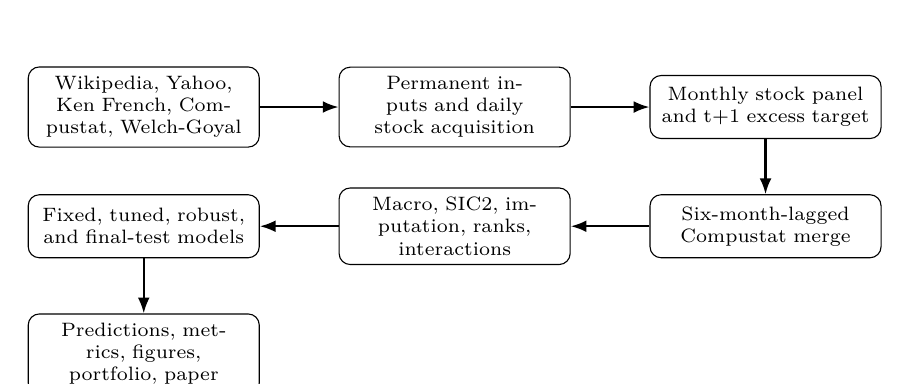
\begin{tikzpicture}[node distance=7mm and 10mm, every node/.style={font=\scriptsize}, box/.style={draw,rounded corners,align=center,minimum height=8mm,text width=27mm}, arr/.style={-{Latex[length=2mm]},thick}]
\node[box] (sources) {Wikipedia, Yahoo, Ken French, Compustat, Welch-Goyal};
\node[box,right=of sources] (inputs) {Permanent inputs and daily stock acquisition};
\node[box,right=of inputs] (monthly) {Monthly stock panel and t+1 excess target};
\node[box,below=of monthly] (fund) {Six-month-lagged Compustat merge};
\node[box,left=of fund] (kelly) {Macro, SIC2, imputation, ranks, interactions};
\node[box,left=of kelly] (models) {Fixed, tuned, robust, and final-test models};
\node[box,below=of models] (report) {Predictions, metrics, figures, portfolio, paper};
\draw[arr] (sources)--(inputs); \draw[arr] (inputs)--(monthly); \draw[arr] (monthly)--(fund); \draw[arr] (fund)--(kelly); \draw[arr] (kelly)--(models); \draw[arr] (models)--(report);
\end{tikzpicture}
\caption{Verified high-level data and output lineage.}
\end{figure}

\section{Data Construction and Timing Decisions}\label{sec-07}

Daily adjusted prices produce simple returns and monthly technical
characteristics. Current month-end information predicts the subsequent
target. Momentum explicitly lags current return. Compustat is delayed
six months and merged backward. Same-month Welch-Goyal values are merged
without the intended one-month shift, and target shifting does not
enforce calendar continuity.

\section{Final Dataset Audit}\label{sec-08}

The final parquet is sorted by ticker and month, has unique column
names, zero missing values, zero infinities, and zero duplicate
ticker-month rows. Its 499 predictors exactly match the predictor
inventory. Near-duplicate predictors were not exhaustively tested
because a complete 499-by-499 dependence audit is computationally
substantial; this is not verifiable from the current repository outputs.

\subsection{Major dataset validation table}\label{sec-dataset-table}

{\def\LTcaptype{none} % do not increment counter
\begin{landscape}
\scriptsize
\begin{longtable}[]{@{}
  >{\raggedright\arraybackslash}p{(\linewidth - 14\tabcolsep) * \real{0.1250}}
  >{\raggedright\arraybackslash}p{(\linewidth - 14\tabcolsep) * \real{0.1250}}
  >{\raggedright\arraybackslash}p{(\linewidth - 14\tabcolsep) * \real{0.1250}}
  >{\raggedright\arraybackslash}p{(\linewidth - 14\tabcolsep) * \real{0.1250}}
  >{\raggedright\arraybackslash}p{(\linewidth - 14\tabcolsep) * \real{0.1250}}
  >{\raggedright\arraybackslash}p{(\linewidth - 14\tabcolsep) * \real{0.1250}}
  >{\raggedright\arraybackslash}p{(\linewidth - 14\tabcolsep) * \real{0.1250}}
  >{\raggedright\arraybackslash}p{(\linewidth - 14\tabcolsep) * \real{0.1250}}@{}}
\toprule\noalign{}
\begin{minipage}[b]{\linewidth}\raggedright
Dataset
\end{minipage} & \begin{minipage}[b]{\linewidth}\raggedright
Path
\end{minipage} & \begin{minipage}[b]{\linewidth}\raggedright
Shape
\end{minipage} & \begin{minipage}[b]{\linewidth}\raggedright
Coverage
\end{minipage} & \begin{minipage}[b]{\linewidth}\raggedright
Entities
\end{minipage} & \begin{minipage}[b]{\linewidth}\raggedright
Missing
\end{minipage} & \begin{minipage}[b]{\linewidth}\raggedright
Duplicates
\end{minipage} & \begin{minipage}[b]{\linewidth}\raggedright
Notes
\end{minipage} \\
\midrule\noalign{}
\endhead
\bottomrule\noalign{}
\endlastfoot
Locked universe & \path{input/stock_universe_locked.csv} & 867 x 1 & n/a
& 867 & 0 & 0 & Permanent Wikipedia-derived current-plus-historical
union \\
Fama-French RF & \path{input/fama_french_rf_monthly.csv} & 1,199 x 2 &
1926-07 to 2026-05 & n/a & 0 & 0 months & RF decimal, month-end \\
GSPC daily & \path{input/market_gspc_daily.csv} & 9,845 x 7 & 1987-01-02
to 2026-01-30 & 1 series & 0 & 0 dates & auto\_\allowbreak{}adjust=False \\
VIX daily & \path{input/market_vix_daily.csv} & 9,087 x 7 & 1990-01-02
to 2026-01-30 & 1 series & 0 & 0 dates & auto\_\allowbreak{}adjust=False \\
Raw Compustat & \path{input/raw/compustat_annual_1980_2025.csv} & 21,575
x 84 & 1980-01-31 to 2026-01-31 & 649 tickers & 148,161 & 0 ticker-date
& Unsorted input; annual statements \\
Welch-Goyal input &
\path{input/external/welch_goyal_macro_1990_2025.csv} & 432 x 10 &
1990-01 to 2025-12 & n/a & 0 & 0 months & Nine values plus month; only
eight are used \\
Clean daily prices &
\path{output/data/final/daily_prices_clean_1987_2026.csv} & 4,701,144 x
8 & 1987-01-02 to 2026-01-30 & 670 & 0 & 0 ticker-date & Sorted \\
Monthly stock panel &
\path{output/data/final/monthly_stock_panel_with_targets_1990_2025.csv}
& 212,794 x 30 & 1990-01 to 2025-12 & 663 & 43,229 & 0 ticker-month & 54
infinities before final cleaning \\
Fundamental panel &
\path{output/data/intermediate/monthly_panel_with_compustat_macro_1990_2025.csv}
& 212,794 x 61 & 1990-01 to 2025-12 & 663 & 497,813 & 0 ticker-month &
207,739 matched rows; no lag violation \\
Raw Kelly panel &
\path{output/data/final/model_dataset_kelly_raw_full_1990_2025.csv} &
212,794 x 126 & 1990-01 to 2025-12 & 663 & 482,648 & 0 ticker-month &
123 base predictors \\
Ranked model panel &
\path{output/data/final/model_dataset_kelly_ranked_full_1990_2025.parquet}
& 212,794 x 502 & 1990-01 to 2025-12 & 663 & 0 & 0 ticker-month & 499
predictors; no infinities \\
Final test predictions &
\path{output/models/test/final_test_predictions.parquet} & 268,968 x 6 &
2020-01 to 2025-12 & 645 & 0 & 0 ticker-month-model & 44,828 rows per
six models \\
\end{longtable}
\end{landscape}
\normalsize
}

The final target has mean 0.0129067, standard deviation 0.109243, median
0.0108016, 1st percentile -0.262064, 99th percentile 0.325020, minimum
-0.935113, and maximum 2.920526. The target is intentionally not
winsorized.

\section{Modeling Framework}\label{sec-09}

Linear models use StandardScaler within sklearn pipelines. Trees use raw
transformed predictors. Tuning minimizes annual-fold average monthly
MSE. Models are compared against a historical mean, and final models are
refit on all 1990-2019 development observations before 2020-2025
prediction.

\section{Model-by-Model Documentation}\label{sec-10}

The historical mean is the development target average. OLS-3 uses size,
book-to-market, and 12-month momentum. PLS uses one selected component.
Elastic Net uses alpha 0.01 and l1 ratio 0.9 and yields zero
coefficients. The selected Decision Tree has depth 3 and minimum leaf
1,000; the selected Random Forest has 200 depth-2 trees, minimum leaf
100, and square-root feature sampling. Gradient Boosting exists only in
legacy archives.

\section{Validation and Test Design}\label{sec-11}

The code uses train 1990-2014, preliminary validation 2015-2019,
development 1990-2019, and test 2020-2025. Hyperparameter grids run only
on train with validation years 2005-2014. Optimized models are then
checked on 2015-2019. This is leakage-resistant but differs from the
active README claim that tuning folds extend through 2019.

\subsection{Split counts}\label{sec-split-counts}

{\def\LTcaptype{none} % do not increment counter
\begin{longtable}[]{@{}lllll@{}}
\toprule\noalign{}
Sample & Rows & Months & Tickers & Dates \\
\midrule\noalign{}
\endhead
\bottomrule\noalign{}
\endlastfoot
Train & 132,336 & 300 & 578 & 1990-01 to 2014-12 \\
Validation & 35,630 & 60 & 618 & 2015-01 to 2019-12 \\
Development & 167,966 & 360 & 620 & 1990-01 to 2019-12 \\
Test & 44,828 & 72 & 645 & 2020-01 to 2025-12 \\
\end{longtable}
}

\section{Results}\label{sec-12}

PLS is numerically best by final monthly MSE and OOS R-squared. The
improvement over the historical mean is very small. Random Forest has
the lowest MAE among the six. Decision Tree is decisively worst.
Validation optimization helps PLS, Elastic Net, and Decision Tree
relative to their fixed forms, but makes Random Forest slightly worse.

\subsection{Frozen final-test comparison}\label{sec-final-results}

{\def\LTcaptype{none} % do not increment counter
\begin{landscape}
\scriptsize
\begin{longtable}[]{@{}
  >{\raggedright\arraybackslash}p{(\linewidth - 12\tabcolsep) * \real{0.1429}}
  >{\raggedright\arraybackslash}p{(\linewidth - 12\tabcolsep) * \real{0.1429}}
  >{\raggedright\arraybackslash}p{(\linewidth - 12\tabcolsep) * \real{0.1429}}
  >{\raggedright\arraybackslash}p{(\linewidth - 12\tabcolsep) * \real{0.1429}}
  >{\raggedright\arraybackslash}p{(\linewidth - 12\tabcolsep) * \real{0.1429}}
  >{\raggedright\arraybackslash}p{(\linewidth - 12\tabcolsep) * \real{0.1429}}
  >{\raggedright\arraybackslash}p{(\linewidth - 12\tabcolsep) * \real{0.1429}}@{}}
\toprule\noalign{}
\begin{minipage}[b]{\linewidth}\raggedright
Rank
\end{minipage} & \begin{minipage}[b]{\linewidth}\raggedright
Model
\end{minipage} & \begin{minipage}[b]{\linewidth}\raggedright
Monthly MSE
\end{minipage} & \begin{minipage}[b]{\linewidth}\raggedright
RMSE
\end{minipage} & \begin{minipage}[b]{\linewidth}\raggedright
MAE
\end{minipage} & \begin{minipage}[b]{\linewidth}\raggedright
OOS R2
\end{minipage} & \begin{minipage}[b]{\linewidth}\raggedright
Correlation
\end{minipage} \\
\midrule\noalign{}
\endhead
\bottomrule\noalign{}
\endlastfoot
1 & PLS & 0.0137866 & 0.1171849 & 0.0801883 & 0.0017914 & 0.0438813 \\
2 & Random Forest & 0.0138037 & 0.1172563 & 0.0800818 & 0.0005754 &
0.0214511 \\
3 & OLS-3 & 0.0138049 & 0.1172615 & 0.0801398 & 0.0004857 & 0.0256182 \\
4 & Elastic Net & 0.0138120 & 0.1172900 & 0.0800774 & approximately 0 &
undefined \\
5 & Historical Mean & 0.0138120 & 0.1172900 & 0.0800774 & approximately
0 & undefined \\
6 & Decision Tree & 0.0156624 & 0.1248378 & 0.0848455 & -0.1328434 &
-0.1453403 \\
\end{longtable}
\end{landscape}
\normalsize
}

Source: \path{output/models/test/final_test_model_comparison.csv},
reproduced in
\path{output/models/interpretation/final_prediction_results.csv}.
Metrics recomputed from
\path{output/models/test/final_test_predictions.parquet} differ by no
more than 7.5e-11.

\begin{figure}
\centering

\includegraphics[width=0.85\linewidth,height=\textheight,keepaspectratio,alt={Final-test monthly MSE by model. Existing frozen figure; not regenerated for this audit.}]{../../output/models/interpretation/figures/test_monthly_mse_by_model.png}
\caption{Final-test monthly MSE by model. Existing frozen figure; not
regenerated for this audit.}
\end{figure}

\begin{figure}
\centering
\includegraphics[width=0.85\linewidth,height=\textheight,keepaspectratio,alt={Final-test OOS R-squared by model. Existing frozen figure; not regenerated for this audit.}]{../../output/models/interpretation/figures/test_oos_r2_by_model.png}
\caption{Final-test OOS R-squared by model. Existing frozen figure; not
regenerated for this audit.}
\end{figure}

\section{Interpretation}\label{sec-13}

Small positive OOS R-squared means a tiny reduction in squared forecast
error relative to the constant benchmark, not that return variation is
well explained. Negative OOS R-squared means the benchmark wins. Elastic
Net's zero solution indicates the chosen penalty finds no stable
incremental signal. Tree impurity importance is predictive and
model-specific, not causal. PLS coefficients describe a supervised
latent projection after standardization and should not be interpreted as
structural premia.

\section{What Was Done Well}\label{sec-14}

Verified strengths include chronological sorting, month-end
normalization, time-separated samples, training-only pipeline scaling,
explicit historical-mean comparison, six-month accounting delay,
backward as-of merging with zero violations, permanent local small
inputs, saved predictor inventories, integrity checks, multiple model
families, frozen interpretation artifacts, and honest negative findings.

\section{Limitations and Questionable Choices}\label{sec-15}

Material limitations include the 26 target continuity failures, unlagged
macro merge, public ticker-based universe and matching, Yahoo
revision/delisting limitations, 499-dimensional design, unwinsorized
squared-loss sensitivity, weak and unstable gains, a poor single tree,
zero Elastic Net solution, unpinned dependencies, stale execution
wrapper, duplicate/legacy artifacts, no formal loss test, and no fully
specified transaction-cost implementation in the main paper.

\section{Leakage and Look-Ahead-Bias Audit}\label{sec-16}

No direct test leakage was found in scaler fitting, hyperparameter
selection, Compustat merging, or final model training. The principal
timing concern is same-month macro availability. The target is future by
construction, but gap transitions sometimes extend beyond one month.
Human adherence to an untouched-test protocol cannot be reconstructed
from files after the test outputs exist.

\subsection{Verification matrix}\label{sec-verification-matrix}

{\def\LTcaptype{none} % do not increment counter
\begin{longtable}[]{@{}
  >{\raggedright\arraybackslash}p{(\linewidth - 6\tabcolsep) * \real{0.2500}}
  >{\raggedright\arraybackslash}p{(\linewidth - 6\tabcolsep) * \real{0.2500}}
  >{\raggedright\arraybackslash}p{(\linewidth - 6\tabcolsep) * \real{0.2500}}
  >{\raggedright\arraybackslash}p{(\linewidth - 6\tabcolsep) * \real{0.2500}}@{}}
\toprule\noalign{}
\begin{minipage}[b]{\linewidth}\raggedright
No.
\end{minipage} & \begin{minipage}[b]{\linewidth}\raggedright
Design point
\end{minipage} & \begin{minipage}[b]{\linewidth}\raggedright
Status
\end{minipage} & \begin{minipage}[b]{\linewidth}\raggedright
Evidence
\end{minipage} \\
\midrule\noalign{}
\endhead
\bottomrule\noalign{}
\endlastfoot
1 & Next-month stock excess-return target & Partially verified & Formula
is stock next-observation return minus next RF; 26 nonconsecutive
transitions. \\
2 & Time-aware shifting & Partially verified & Sorted group shift(-1),
but no calendar-continuity guard. \\
3 & Sort before group shifts & Verified & Data file 02 sorts
ticker/month before shifts. \\
4 & Predictor timing & Partially verified & Stock and Compustat timing
mostly sound; macro lag is unresolved/inconsistent. \\
5 & Month-end dates & Verified & All audited monthly inputs and panels
are month-end. \\
6 & Decimal returns & Verified & RF ranges 0 to 0.0069 and return
magnitudes are decimal simple returns. \\
7 & Daily returns for volatility & Verified & Daily adjusted-close
percentage changes feed monthly and rolling volatility. \\
8 & Monthly adjusted-close return & Verified & Last monthly adjusted
close percentage change. \\
9 & Rolling features historical only & Partially verified & Momentum is
lagged; contemporaneous month-end variables are used for t+1, as
intended. \\
10 & 36-month history & Partially verified & min\_\allowbreak{}periods=36, but the
window counts observations and missing months are not explicitly
checked. \\
11 & Six-month Compustat lag & Verified & 207,739 matched rows and zero
saved timing violations. \\
12 & Backward Compustat as-of merge & Verified & direction=`backward' by
ticker. \\
13 & No future Compustat reports & Verified & Zero
comp\_\allowbreak{}available\_\allowbreak{}month \textgreater{} stock month violations. \\
14 & Macro variables appropriately lagged & Inconsistent & Active code
merges same-month values; intended one-month lag absent. \\
15 & Fama-French alignment & Verified & Month-end RF shifted one row;
monthly input is unique and decimal. \\
16 & Market/VIX are market-wide & Verified & At most one value per month
across tickers for all four variables. \\
17 & Predictors lagged where required & Partially verified & Target and
momentum timing explicit; macro publication timing unresolved. \\
18 & Training-only standardization & Verified & StandardScaler is inside
each fitted sklearn pipeline. \\
19 & No validation/test scaler fit & Verified & Pipeline fit occurs on
fold training, train, or development arrays only. \\
20 & Chronological rather than random CV & Verified & Annual expanding
masks use years \textless{} validation year. \\
21 & Expanding folds use earlier data & Verified & 1990-2004
-\textgreater{} 2005 through 1990-2013 -\textgreater{} 2014 in actual
tuning. \\
22 & Hyperparameters exclude test & Verified & Tuning loads train only;
final script only reads saved parameters. \\
23 & Test not used for tuning & Verified in code & Human viewing history
is not verifiable from current repository. \\
24 & Final test untouched until evaluation & Not verifiable & Code
separates it, but procedural history cannot be proven. \\
25 & Predictor file matches model columns & Verified & 499 unique names
exactly equal parquet columns after identifiers/target. \\
26 & Identifiers and target excluded & Verified & Predictor list begins
after ticker, month, target. \\
27 & Missing handling consistent & Verified for final panel & Monthly
median then zero; final missing count is zero. \\
28 & No duplicate ticker-month rows & Verified & Zero in monthly, raw,
and ranked panels. \\
29 & Documented dataset dimensions & Verified for generated summaries &
212,794 x 502 and 499 predictors match output metadata. \\
30 & Result tables match predictions & Verified & Recomputed
discrepancies below 7.5e-11. \\
31 & Figures match frozen results & Verified by lineage/timestamps & All
figures are newer than source result tables. \\
32 & Paper values consistent & Verified for direct-linked tables &
Current paper reads frozen CSV/PNG outputs and is newer than figures. \\
33 & Random seeds consistent & Partially verified & 42 is used for
stochastic active models; PLS/OLS deterministic. \\
34 & Fixed/optimized naming & Verified in outputs & Suffixes are
consistent; final test removes suffixes deliberately. \\
35 & Historical mean uses allowable data & Verified & Final constant
equals development mean up to float32 precision. \\
\end{longtable}
}

\section{Reproducibility Audit}\label{sec-17}

Data steps are mostly explicit and canonical paths are centralized.
Reproducibility is weakened by online per-ticker Yahoo downloads, an
unscripted Compustat extraction, absolute manifest paths, unpinned
packages, no lock file, missing shell targets, absent tests, and no
recorded runtime/provenance hashes. Existing outputs permit result
reproduction without retraining, but not proof that they came from the
current exact source state.

\section{Consistency and Staleness Audit}\label{sec-18}

Final metrics recomputed from predictions agree within floating
precision, the ranking order is correct, figures are newer than source
result tables, and the paper is newer than figures. Inconsistencies are
concentrated in workflow documentation, shell paths, duplicated
input/legacy files, orphan bytecode, and intended versus actual
macro/tuning logic.

\subsection{Evidence-supported inconsistency
register}\label{sec-issue-register}

{\def\LTcaptype{none} % do not increment counter
\begin{landscape}
\scriptsize
\begin{longtable}[]{@{}
  >{\raggedright\arraybackslash}p{(\linewidth - 10\tabcolsep) * \real{0.1667}}
  >{\raggedright\arraybackslash}p{(\linewidth - 10\tabcolsep) * \real{0.1667}}
  >{\raggedright\arraybackslash}p{(\linewidth - 10\tabcolsep) * \real{0.1667}}
  >{\raggedright\arraybackslash}p{(\linewidth - 10\tabcolsep) * \real{0.1667}}
  >{\raggedright\arraybackslash}p{(\linewidth - 10\tabcolsep) * \real{0.1667}}
  >{\raggedright\arraybackslash}p{(\linewidth - 10\tabcolsep) * \real{0.1667}}@{}}
\toprule\noalign{}
\begin{minipage}[b]{\linewidth}\raggedright
ID
\end{minipage} & \begin{minipage}[b]{\linewidth}\raggedright
Severity
\end{minipage} & \begin{minipage}[b]{\linewidth}\raggedright
Dimension
\end{minipage} & \begin{minipage}[b]{\linewidth}\raggedright
Issue
\end{minipage} & \begin{minipage}[b]{\linewidth}\raggedright
Evidence
\end{minipage} & \begin{minipage}[b]{\linewidth}\raggedright
Recommended check
\end{minipage} \\
\midrule\noalign{}
\endhead
\bottomrule\noalign{}
\endlastfoot
I01 & High & Validity & 26 targets cross gaps and are not
next-calendar-month returns & Monthly panel plus data file 02 shift(-1)
& Require the next observed month to equal month+1 before assigning
target \\
I02 & High & Validity & Same-month macro merge contradicts intended
one-month lag & data file 04:62-84 & Verify publication timing and lag
macro inputs explicitly \\
I03 & High & Reproducibility & run\_\allowbreak{}pipeline.sh calls five missing
scripts & Direct existence check & Update wrapper after deciding
canonical stages \\
I04 & High & Reproducibility & README tuning period and
one-standard-error claim do not match code & models README versus
tuning/estimation code & Correct documentation or implementation \\
I05 & Medium & Reproducibility & Failed Yahoo downloads are printed but
not persisted & data file 01 main & Save an acquisition failure
report \\
I06 & Medium & Validity & Wikipedia union cannot guarantee point-in-time
membership or delisting returns & Universe acquisition logic & Use CRSP
permanent identifiers for a future version \\
I07 & Medium & Validity & Ticker-based Compustat-Yahoo merge risks
symbol-change mismatches & data file 03 & Audit permanent identifier
mapping \\
I08 & Medium & Interpretation & 499 predictors include 376 interactions
& Cleaning summary & Report regularization burden and run
lower-dimensional sensitivity \\
I09 & Medium & Interpretation & Unwinsorized target contains 91
observations above 100\% absolute return & extreme\_\allowbreak{}target\_\allowbreak{}counts.csv &
Report robustness to robust loss or documented winsorization \\
I10 & Medium & Empirical credibility & No formal forecast-loss
comparison test & No active test file found & Add Diebold-Mariano or
panel-aware resampling in future \\
I11 & Medium & Economic interpretation & Portfolio outputs exist but
current paper focuses mostly on prediction & output/models/portfolio
versus thesis & Decide whether portfolio evidence is in scope and
discuss costs \\
I12 & Medium & Reproducibility & requirements are unpinned and Python
version is unspecified & requirements.txt & Lock package and Python
versions \\
I13 & Medium & Reproducibility & Input manifest stores machine-specific
absolute paths & input/input\_\allowbreak{}manifest.csv & Store repository-relative
paths \\
I14 & Medium & Staleness & Source caches remain for deleted scripts &
orphan pyc inventory & Remove caches from submissions; do not treat them
as source \\
I15 & Low & Organization & Identical Fama-French RF files exist in
input/ and input/external/ & Matching SHA-1 & Keep one canonical copy
after confirming consumers \\
I16 & Low & Organization & Large legacy and backup trees duplicate old
model logic and outputs & backup/ and legacy/ & Exclude from submission
archive or label clearly \\
I17 & Medium & Reproducibility & No automated unit-test suite is present
& Repository tree & Add tests for target continuity, lags, folds, and
metrics \\
I18 & Low & Presentation & Existing thesis build auxiliaries and OS
metadata are present & thesis/*.aux etc. and .DS\_\allowbreak{}Store & Clean
submission artifact directories \\
I19 & Medium & Data quality & 54 infinities exist before final cleaning
& Dataset scan & Document affected columns and assert replacement before
imputation \\
I20 & Medium & Methodology & Beta/idio-vol formula is a rolling variance
identity, not an explicit regression with intercept & data file
02:306-321 & Clarify definition or compare with rolling OLS \\
I21 & Low & Presentation & Existing bibliography contains an unresolved
course-reference comment & thesis/references.bib & Verify required
course citations before submission \\
I22 & Medium & Process & Untouched-test discipline cannot be proven from
code after results exist & Repository state & Describe the procedural
claim cautiously \\
\end{longtable}
\end{landscape}
\normalsize
}

\section{Required Checks Before Submission}\label{sec-19}

The priority is to verify target calendar continuity and macro
publication timing, repair the run instructions, align the
methodological description with actual folds and selection rule, confirm
required citations, state the universe/ticker limitations, and decide
whether the portfolio evidence is in scope. These checks should be
completed before claiming a fully reproducible and leakage-safe
submission.

\section{Recommended Future Improvements}\label{sec-20}

Use point-in-time CRSP/Compustat identifiers and delisting returns,
actual filing dates, explicit macro release lags, a calendar-grid
target, locked environments, automated tests, provenance hashes, nested
or repeated chronological validation, robust-loss sensitivity, formal
forecast-comparison inference, and a prespecified net-of-cost portfolio
design.

\section{Final Overall Assessment}\label{sec-21}

The project is methodologically thoughtful and unusually transparent for
a course project, but it requires important checks before submission.
The core result - weak predictability with several model failures - is
credible as a negative finding. Strong claims about a strict one-month
target, macro timing, complete reproducibility, or profitability are not
yet justified.

\subsection{Scorecard}\label{sec-scorecard}

{\def\LTcaptype{none} % do not increment counter
\begin{longtable}[]{@{}
  >{\raggedright\arraybackslash}p{(\linewidth - 4\tabcolsep) * \real{0.3333}}
  >{\raggedright\arraybackslash}p{(\linewidth - 4\tabcolsep) * \real{0.3333}}
  >{\raggedright\arraybackslash}p{(\linewidth - 4\tabcolsep) * \real{0.3333}}@{}}
\toprule\noalign{}
\begin{minipage}[b]{\linewidth}\raggedright
Category
\end{minipage} & \begin{minipage}[b]{\linewidth}\raggedright
Score / 10
\end{minipage} & \begin{minipage}[b]{\linewidth}\raggedright
Reason
\end{minipage} \\
\midrule\noalign{}
\endhead
\bottomrule\noalign{}
\endlastfoot
Methodological quality & 7 & Strong chronology and benchmarks; target
continuity and macro lag require correction \\
Data quality & 6 & Large transparent panel; public-vendor and
ticker-history limitations \\
Leakage protection & 8 & Scaler, test, and Compustat protections
verified; macro timing unresolved \\
Reproducibility & 5 & Frozen outputs and central config help; wrapper,
versions, and Compustat extraction hinder \\
Code organization & 7 & Clear stages/utilities; archives, stale paths,
and caches create ambiguity \\
Documentation & 6 & Substantial guides and paper; tuning claims drift
from code \\
Empirical credibility & 7 & Negative findings are honest; no formal loss
test and gains are tiny \\
Submission readiness & 6 & Requires important checks before
submission \\
\end{longtable}
}

\textbf{Final verdict: Requires important checks.}

\subsubsection{Top ten strongest
aspects}\label{top-ten-strongest-aspects}

\begin{enumerate}
\def\labelenumi{\arabic{enumi}.}
\tightlist
\item
  Chronological train/validation/development/test separation.
\item
  Training-only pipeline standardization.
\item
  Verified six-month Compustat lag.
\item
  Verified backward as-of merge.
\item
  Permanent local small external inputs.
\item
  Exact predictor inventory.
\item
  Multiple transparent benchmarks and model families.
\item
  Frozen predictions and recomputable metrics.
\item
  Honest reporting of weak and negative results.
\item
  Interpretation, diagnostics, robustness, and portfolio artifacts.
\end{enumerate}

\subsubsection{Top ten weaknesses}\label{top-ten-weaknesses}

\begin{enumerate}
\def\labelenumi{\arabic{enumi}.}
\tightlist
\item
  Twenty-six non-calendar target transitions.
\item
  Same-month macro merge.
\item
  Stale shell workflow.
\item
  Tuning documentation mismatch.
\item
  Unpinned environment.
\item
  Public ticker universe and matching.
\item
  Unscripted Compustat extraction.
\item
  High interaction dimensionality.
\item
  No formal forecast-loss test.
\item
  No proof of historical untouched-test discipline.
\end{enumerate}

\section{Reproduction Guide}\label{sec-22}

Three reproducibility levels are possible: rebuild all data (requires
network access and the supplied Compustat CSV), rerun models from the
final parquet, or regenerate interpretation and paper artifacts only.
Because run\_\allowbreak{}pipeline.sh is stale, the canonical manual order in this
report should be followed until the wrapper is corrected.

\subsection{Required environment}\label{sec-environment}

The repository lists pandas, numpy, scikit-learn, statsmodels, requests,
yfinance, pyarrow, matplotlib, openpyxl. The inspected environment is
Python 3.13.2 with pandas 2.3.3, numpy 2.2.3, scikit-learn 1.8.0,
statsmodels 0.14.5, requests 2.32.3, yfinance 1.4.1, pyarrow 19.0.1,
matplotlib 3.10.1, and openpyxl 3.1.5. These are observations, not
locked requirements. WRDS credentials are required only to recreate the
Compustat extraction, whose query is absent. Wikipedia/Yahoo/Ken French
access is required for acquisition. No FRED API is used.

\subsection{Three run levels}\label{sec-run-levels}

\textbf{Raw rebuild:} run acquisition scripts as needed, provide raw
Compustat, then data files 01-05. This downloads large stock histories
and was not executed during this audit.

\textbf{Model-only rebuild:} with the final parquet and predictor CSV
present, run fixed, tuning, optimized comparison, robustness, final
test, then interpretation using the active paths documented above. Do
not rely on the current shell wrapper.

\textbf{Reporting-only rebuild:} run
\texttt{python\ src/models/step\_\allowbreak{}06\_\allowbreak{}interpretation/run\_\allowbreak{}all.py} only if
frozen test/validation inputs are already present, then compile
\texttt{thesis/paper.tex} with its Makefile.

\section{Glossary}\label{sec-23}

Key terms: adjusted close (split/dividend-adjusted price); OOS R2
(benchmark-relative squared-error improvement); monthly MSE
(equal-weighted mean of within-month MSE); PLS (partial least squares);
RF (risk-free rate or, when named as a model, Random Forest); SIC2
(two-digit industry code); expanding window (all prior years train the
next year); development sample (all pre-test observations).

\appendix

\section{Full Directory Tree}\label{app-tree}

The tree is a complete pre-audit snapshot excluding \texttt{.git} and
the newly created audit directory.

\begin{Shaded}
\begin{Highlighting}[]
\NormalTok{.DS\_\allowbreak{}Store}
\NormalTok{.gitignore}
\NormalTok{.matplotlib/fontlist{-}v390.json}
\NormalTok{README.md}
\NormalTok{backup/model\_\allowbreak{}reorganization\_\allowbreak{}20260719\_\allowbreak{}054538/audit\_\allowbreak{}report.txt}
\NormalTok{backup/model\_\allowbreak{}reorganization\_\allowbreak{}20260719\_\allowbreak{}054538/existing\_\allowbreak{}output\_\allowbreak{}files.txt}
\NormalTok{backup/model\_\allowbreak{}reorganization\_\allowbreak{}20260719\_\allowbreak{}054538/original\_\allowbreak{}directory\_\allowbreak{}tree.txt}
\NormalTok{backup/model\_\allowbreak{}reorganization\_\allowbreak{}20260719\_\allowbreak{}054538/src/models/step\_\allowbreak{}01\_\allowbreak{}fixed/01\_\allowbreak{}fixed\_\allowbreak{}linear\_\allowbreak{}models.py}
\NormalTok{backup/model\_\allowbreak{}reorganization\_\allowbreak{}20260719\_\allowbreak{}054538/src/models/step\_\allowbreak{}01\_\allowbreak{}fixed/02\_\allowbreak{}fixed\_\allowbreak{}tree\_\allowbreak{}models.py}
\NormalTok{backup/model\_\allowbreak{}reorganization\_\allowbreak{}20260719\_\allowbreak{}054538/src/models/step\_\allowbreak{}01\_\allowbreak{}fixed/03\_\allowbreak{}compare\_\allowbreak{}fixed\_\allowbreak{}models.py}
\NormalTok{backup/model\_\allowbreak{}reorganization\_\allowbreak{}20260719\_\allowbreak{}054538/src/models/step\_\allowbreak{}03\_\allowbreak{}optimization/01\_\allowbreak{}optimized\_\allowbreak{}linear\_\allowbreak{}models.py}
\NormalTok{backup/model\_\allowbreak{}reorganization\_\allowbreak{}20260719\_\allowbreak{}054538/src/models/step\_\allowbreak{}03\_\allowbreak{}optimization/02\_\allowbreak{}optimized\_\allowbreak{}tree\_\allowbreak{}models.py}
\NormalTok{backup/model\_\allowbreak{}reorganization\_\allowbreak{}20260719\_\allowbreak{}054538/src/models/step\_\allowbreak{}03\_\allowbreak{}optimization/03\_\allowbreak{}compare\_\allowbreak{}optimized\_\allowbreak{}models.py}
\NormalTok{backup/model\_\allowbreak{}reorganization\_\allowbreak{}20260719\_\allowbreak{}054538/src/models/step\_\allowbreak{}03\_\allowbreak{}optimization/04\_\allowbreak{}compare\_\allowbreak{}fixed\_\allowbreak{}vs\_\allowbreak{}optimized.py}
\NormalTok{backup/model\_\allowbreak{}reorganization\_\allowbreak{}20260719\_\allowbreak{}054538/src/models/utils/estimation.py}
\NormalTok{backup/model\_\allowbreak{}reorganization\_\allowbreak{}20260719\_\allowbreak{}054538/src/models/utils/evaluation.py}
\NormalTok{backup/remove\_\allowbreak{}gradient\_\allowbreak{}boosting\_\allowbreak{}20260719\_\allowbreak{}063836/gradient\_\allowbreak{}boosting\_\allowbreak{}inventory.txt}
\NormalTok{backup/remove\_\allowbreak{}gradient\_\allowbreak{}boosting\_\allowbreak{}20260719\_\allowbreak{}063836/src/models/README.md}
\NormalTok{backup/remove\_\allowbreak{}gradient\_\allowbreak{}boosting\_\allowbreak{}20260719\_\allowbreak{}063836/src/models/README\_\allowbreak{}MODEL\_\allowbreak{}WORKFLOW.md}
\NormalTok{backup/remove\_\allowbreak{}gradient\_\allowbreak{}boosting\_\allowbreak{}20260719\_\allowbreak{}063836/src/models/step\_\allowbreak{}01\_\allowbreak{}fixed/02\_\allowbreak{}fixed\_\allowbreak{}tree\_\allowbreak{}models.py}
\NormalTok{backup/remove\_\allowbreak{}gradient\_\allowbreak{}boosting\_\allowbreak{}20260719\_\allowbreak{}063836/src/models/step\_\allowbreak{}01\_\allowbreak{}fixed/03\_\allowbreak{}compare\_\allowbreak{}fixed\_\allowbreak{}models.py}
\NormalTok{backup/remove\_\allowbreak{}gradient\_\allowbreak{}boosting\_\allowbreak{}20260719\_\allowbreak{}063836/src/models/step\_\allowbreak{}02\_\allowbreak{}tuning/02\_\allowbreak{}tune\_\allowbreak{}tree\_\allowbreak{}models.py}
\NormalTok{backup/remove\_\allowbreak{}gradient\_\allowbreak{}boosting\_\allowbreak{}20260719\_\allowbreak{}063836/src/models/step\_\allowbreak{}02\_\allowbreak{}tuning/03\_\allowbreak{}compare\_\allowbreak{}tuning\_\allowbreak{}results.py}
\NormalTok{backup/remove\_\allowbreak{}gradient\_\allowbreak{}boosting\_\allowbreak{}20260719\_\allowbreak{}063836/src/models/step\_\allowbreak{}03\_\allowbreak{}optimization/02\_\allowbreak{}optimized\_\allowbreak{}tree\_\allowbreak{}models.py}
\NormalTok{backup/remove\_\allowbreak{}gradient\_\allowbreak{}boosting\_\allowbreak{}20260719\_\allowbreak{}063836/src/models/step\_\allowbreak{}03\_\allowbreak{}optimization/03\_\allowbreak{}compare\_\allowbreak{}optimized\_\allowbreak{}models.py}
\NormalTok{backup/remove\_\allowbreak{}gradient\_\allowbreak{}boosting\_\allowbreak{}20260719\_\allowbreak{}063836/src/models/step\_\allowbreak{}03\_\allowbreak{}optimization/04\_\allowbreak{}compare\_\allowbreak{}fixed\_\allowbreak{}vs\_\allowbreak{}optimized.py}
\NormalTok{backup/remove\_\allowbreak{}gradient\_\allowbreak{}boosting\_\allowbreak{}20260719\_\allowbreak{}063836/src/models/step\_\allowbreak{}04\_\allowbreak{}robustness/01\_\allowbreak{}time\_\allowbreak{}series\_\allowbreak{}robustness.py}
\NormalTok{backup/remove\_\allowbreak{}gradient\_\allowbreak{}boosting\_\allowbreak{}20260719\_\allowbreak{}063836/src/models/step\_\allowbreak{}05\_\allowbreak{}test/01\_\allowbreak{}final\_\allowbreak{}test\_\allowbreak{}evaluation.py}
\NormalTok{backup/remove\_\allowbreak{}gradient\_\allowbreak{}boosting\_\allowbreak{}20260719\_\allowbreak{}063836/src/models/step\_\allowbreak{}06\_\allowbreak{}portfolio/01\_\allowbreak{}portfolio\_\allowbreak{}sorts.py}
\NormalTok{backup/remove\_\allowbreak{}gradient\_\allowbreak{}boosting\_\allowbreak{}20260719\_\allowbreak{}063836/src/models/step\_\allowbreak{}06\_\allowbreak{}portfolio/02\_\allowbreak{}compare\_\allowbreak{}portfolio\_\allowbreak{}results.py}
\NormalTok{backup/remove\_\allowbreak{}gradient\_\allowbreak{}boosting\_\allowbreak{}20260719\_\allowbreak{}063836/src/models/step\_\allowbreak{}06\_\allowbreak{}portfolio/03\_\allowbreak{}final\_\allowbreak{}model\_\allowbreak{}and\_\allowbreak{}portfolio\_\allowbreak{}summary.py}
\NormalTok{docs/Data\_\allowbreak{}Construction\_\allowbreak{}Guide.pdf}
\NormalTok{docs/Data\_\allowbreak{}Construction\_\allowbreak{}Guide.tex}
\NormalTok{docs/Pipeline\_\allowbreak{}Overview.pdf}
\NormalTok{docs/figures/.gitkeep}
\NormalTok{input/.DS\_\allowbreak{}Store}
\NormalTok{input/README.md}
\NormalTok{input/external/.DS\_\allowbreak{}Store}
\NormalTok{input/external/.gitkeep}
\NormalTok{input/external/fama\_\allowbreak{}french\_\allowbreak{}rf\_\allowbreak{}monthly.csv}
\NormalTok{input/external/welch\_\allowbreak{}goyal\_\allowbreak{}macro\_\allowbreak{}1990\_\allowbreak{}2025.csv}
\NormalTok{input/fama\_\allowbreak{}french\_\allowbreak{}rf\_\allowbreak{}monthly.csv}
\NormalTok{input/input\_\allowbreak{}manifest.csv}
\NormalTok{input/market\_\allowbreak{}gspc\_\allowbreak{}daily.csv}
\NormalTok{input/market\_\allowbreak{}vix\_\allowbreak{}daily.csv}
\NormalTok{input/raw/.DS\_\allowbreak{}Store}
\NormalTok{input/raw/.gitkeep}
\NormalTok{input/raw/compustat\_\allowbreak{}annual\_\allowbreak{}1980\_\allowbreak{}2025.csv}
\NormalTok{input/stock\_\allowbreak{}universe\_\allowbreak{}locked.csv}
\NormalTok{output/data/final/cleaning\_\allowbreak{}summary.csv}
\NormalTok{output/data/final/daily\_\allowbreak{}prices\_\allowbreak{}clean\_\allowbreak{}1987\_\allowbreak{}2026.csv}
\NormalTok{output/data/final/dropped\_\allowbreak{}predictors\_\allowbreak{}empty.csv}
\NormalTok{output/data/final/extreme\_\allowbreak{}target\_\allowbreak{}counts.csv}
\NormalTok{output/data/final/extreme\_\allowbreak{}target\_\allowbreak{}observations.csv}
\NormalTok{output/data/final/kelly\_\allowbreak{}raw\_\allowbreak{}dataset\_\allowbreak{}summary.csv}
\NormalTok{output/data/final/model\_\allowbreak{}dataset\_\allowbreak{}kelly\_\allowbreak{}ranked\_\allowbreak{}full\_\allowbreak{}1990\_\allowbreak{}2025.parquet}
\NormalTok{output/data/final/model\_\allowbreak{}dataset\_\allowbreak{}kelly\_\allowbreak{}raw\_\allowbreak{}full\_\allowbreak{}1990\_\allowbreak{}2025.csv}
\NormalTok{output/data/final/monthly\_\allowbreak{}imputation\_\allowbreak{}medians\_\allowbreak{}summary.csv}
\NormalTok{output/data/final/monthly\_\allowbreak{}stock\_\allowbreak{}panel\_\allowbreak{}with\_\allowbreak{}targets\_\allowbreak{}1990\_\allowbreak{}2025.csv}
\NormalTok{output/data/final/predictor\_\allowbreak{}columns\_\allowbreak{}kelly\_\allowbreak{}ranked.csv}
\NormalTok{output/data/final/predictor\_\allowbreak{}columns\_\allowbreak{}kelly\_\allowbreak{}raw.csv}
\NormalTok{output/data/final/removed\_\allowbreak{}tickers.csv}
\NormalTok{output/data/final/sp500\_\allowbreak{}tickers\_\allowbreak{}clean.csv}
\NormalTok{output/data/intermediate/compustat\_\allowbreak{}annual\_\allowbreak{}cleaned\_\allowbreak{}1980\_\allowbreak{}2025.csv}
\NormalTok{output/data/intermediate/daily\_\allowbreak{}prices\_\allowbreak{}raw\_\allowbreak{}1987\_\allowbreak{}2026.csv}
\NormalTok{output/data/intermediate/monthly\_\allowbreak{}panel\_\allowbreak{}with\_\allowbreak{}compustat\_\allowbreak{}macro\_\allowbreak{}1990\_\allowbreak{}2025.csv}
\NormalTok{output/data/intermediate/monthly\_\allowbreak{}removed\_\allowbreak{}tickers.csv}
\NormalTok{output/data/intermediate/monthly\_\allowbreak{}return\_\allowbreak{}quality\_\allowbreak{}report.csv}
\NormalTok{output/data/intermediate/sp500\_\allowbreak{}tickers\_\allowbreak{}raw.csv}
\NormalTok{output/data/intermediate/ticker\_\allowbreak{}quality\_\allowbreak{}report.csv}
\NormalTok{output/models/fixed/diagnostics/decision\_\allowbreak{}tree\_\allowbreak{}feature\_\allowbreak{}importance.csv}
\NormalTok{output/models/fixed/diagnostics/decision\_\allowbreak{}tree\_\allowbreak{}rules.txt}
\NormalTok{output/models/fixed/diagnostics/decision\_\allowbreak{}tree\_\allowbreak{}split\_\allowbreak{}feature\_\allowbreak{}distributions.csv}
\NormalTok{output/models/fixed/diagnostics/decision\_\allowbreak{}tree\_\allowbreak{}structure.csv}
\NormalTok{output/models/fixed/diagnostics/decision\_\allowbreak{}tree\_\allowbreak{}train\_\allowbreak{}leaf\_\allowbreak{}distribution.csv}
\NormalTok{output/models/fixed/diagnostics/decision\_\allowbreak{}tree\_\allowbreak{}validation\_\allowbreak{}leaf\_\allowbreak{}distribution.csv}
\NormalTok{output/models/fixed/diagnostics/diagnostic\_\allowbreak{}warning\_\allowbreak{}summary.csv}
\NormalTok{output/models/fixed/diagnostics/diagnostic\_\allowbreak{}warnings.txt}
\NormalTok{output/models/fixed/diagnostics/extreme\_\allowbreak{}predictions.csv}
\NormalTok{output/models/fixed/diagnostics/fixed\_\allowbreak{}data\_\allowbreak{}summary.csv}
\NormalTok{output/models/fixed/diagnostics/fixed\_\allowbreak{}model\_\allowbreak{}performance\_\allowbreak{}by\_\allowbreak{}month.csv}
\NormalTok{output/models/fixed/diagnostics/fixed\_\allowbreak{}model\_\allowbreak{}performance\_\allowbreak{}by\_\allowbreak{}validation\_\allowbreak{}year.csv}
\NormalTok{output/models/fixed/diagnostics/fixed\_\allowbreak{}prediction\_\allowbreak{}distribution.csv}
\NormalTok{output/models/fixed/diagnostics/largest\_\allowbreak{}absolute\_\allowbreak{}prediction\_\allowbreak{}rows.csv}
\NormalTok{output/models/fixed/diagnostics/largest\_\allowbreak{}absolute\_\allowbreak{}target\_\allowbreak{}rows.csv}
\NormalTok{output/models/fixed/diagnostics/largest\_\allowbreak{}prediction\_\allowbreak{}rows.csv}
\NormalTok{output/models/fixed/diagnostics/largest\_\allowbreak{}target\_\allowbreak{}rows.csv}
\NormalTok{output/models/fixed/diagnostics/ols3\_\allowbreak{}predictor\_\allowbreak{}distribution.csv}
\NormalTok{output/models/fixed/diagnostics/ols3\_\allowbreak{}selected\_\allowbreak{}predictors.csv}
\NormalTok{output/models/fixed/diagnostics/prediction\_\allowbreak{}summary.csv}
\NormalTok{output/models/fixed/diagnostics/predictor\_\allowbreak{}distribution\_\allowbreak{}flags.csv}
\NormalTok{output/models/fixed/diagnostics/predictor\_\allowbreak{}distribution\_\allowbreak{}summary.csv}
\NormalTok{output/models/fixed/diagnostics/random\_\allowbreak{}forest\_\allowbreak{}extreme\_\allowbreak{}predictions.csv}
\NormalTok{output/models/fixed/diagnostics/random\_\allowbreak{}forest\_\allowbreak{}feature\_\allowbreak{}importance.csv}
\NormalTok{output/models/fixed/diagnostics/random\_\allowbreak{}forest\_\allowbreak{}prediction\_\allowbreak{}summary.csv}
\NormalTok{output/models/fixed/diagnostics/smallest\_\allowbreak{}prediction\_\allowbreak{}rows.csv}
\NormalTok{output/models/fixed/diagnostics/smallest\_\allowbreak{}target\_\allowbreak{}rows.csv}
\NormalTok{output/models/fixed/diagnostics/squared\_\allowbreak{}error\_\allowbreak{}concentration.csv}
\NormalTok{output/models/fixed/diagnostics/target\_\allowbreak{}extreme\_\allowbreak{}counts.csv}
\NormalTok{output/models/fixed/diagnostics/target\_\allowbreak{}quantiles.csv}
\NormalTok{output/models/fixed/diagnostics/target\_\allowbreak{}summary.csv}
\NormalTok{output/models/fixed/diagnostics/target\_\allowbreak{}summary\_\allowbreak{}by\_\allowbreak{}month.csv}
\NormalTok{output/models/fixed/diagnostics/target\_\allowbreak{}summary\_\allowbreak{}by\_\allowbreak{}year.csv}
\NormalTok{output/models/fixed/diagnostics/validation\_\allowbreak{}performance\_\allowbreak{}by\_\allowbreak{}year.csv}
\NormalTok{output/models/fixed/fixed\_\allowbreak{}all\_\allowbreak{}model\_\allowbreak{}metrics.csv}
\NormalTok{output/models/fixed/fixed\_\allowbreak{}linear\_\allowbreak{}model\_\allowbreak{}coefficients.csv}
\NormalTok{output/models/fixed/fixed\_\allowbreak{}linear\_\allowbreak{}model\_\allowbreak{}metrics.csv}
\NormalTok{output/models/fixed/fixed\_\allowbreak{}linear\_\allowbreak{}model\_\allowbreak{}predictions.parquet}
\NormalTok{output/models/fixed/fixed\_\allowbreak{}model\_\allowbreak{}summary\_\allowbreak{}wide.csv}
\NormalTok{output/models/fixed/fixed\_\allowbreak{}model\_\allowbreak{}validation\_\allowbreak{}ranking.csv}
\NormalTok{output/models/fixed/fixed\_\allowbreak{}tree\_\allowbreak{}model\_\allowbreak{}feature\_\allowbreak{}importance.csv}
\NormalTok{output/models/fixed/fixed\_\allowbreak{}tree\_\allowbreak{}model\_\allowbreak{}metrics.csv}
\NormalTok{output/models/fixed/fixed\_\allowbreak{}tree\_\allowbreak{}model\_\allowbreak{}predictions.parquet}
\NormalTok{output/models/interpretation/best\_\allowbreak{}hyperparameters.csv}
\NormalTok{output/models/interpretation/decision\_\allowbreak{}tree\_\allowbreak{}feature\_\allowbreak{}importance.csv}
\NormalTok{output/models/interpretation/elastic\_\allowbreak{}net\_\allowbreak{}coefficients.csv}
\NormalTok{output/models/interpretation/feature\_\allowbreak{}importance\_\allowbreak{}top\_\allowbreak{}variables.csv}
\NormalTok{output/models/interpretation/figures/prediction\_\allowbreak{}distribution\_\allowbreak{}by\_\allowbreak{}model.png}
\NormalTok{output/models/interpretation/figures/prediction\_\allowbreak{}vs\_\allowbreak{}realized\_\allowbreak{}pls.png}
\NormalTok{output/models/interpretation/figures/test\_\allowbreak{}correlation\_\allowbreak{}by\_\allowbreak{}model.png}
\NormalTok{output/models/interpretation/figures/test\_\allowbreak{}monthly\_\allowbreak{}mse\_\allowbreak{}by\_\allowbreak{}model.png}
\NormalTok{output/models/interpretation/figures/test\_\allowbreak{}oos\_\allowbreak{}r2\_\allowbreak{}by\_\allowbreak{}model.png}
\NormalTok{output/models/interpretation/figures/top\_\allowbreak{}decision\_\allowbreak{}tree\_\allowbreak{}features.png}
\NormalTok{output/models/interpretation/figures/top\_\allowbreak{}elastic\_\allowbreak{}net\_\allowbreak{}coefficients\_\allowbreak{}skipped.txt}
\NormalTok{output/models/interpretation/figures/top\_\allowbreak{}pls\_\allowbreak{}coefficients.png}
\NormalTok{output/models/interpretation/figures/top\_\allowbreak{}random\_\allowbreak{}forest\_\allowbreak{}features.png}
\NormalTok{output/models/interpretation/figures/yearly\_\allowbreak{}mse\_\allowbreak{}by\_\allowbreak{}model.png}
\NormalTok{output/models/interpretation/figures/yearly\_\allowbreak{}oos\_\allowbreak{}r2\_\allowbreak{}by\_\allowbreak{}model.png}
\NormalTok{output/models/interpretation/final\_\allowbreak{}model\_\allowbreak{}complexity.csv}
\NormalTok{output/models/interpretation/final\_\allowbreak{}prediction\_\allowbreak{}results.csv}
\NormalTok{output/models/interpretation/final\_\allowbreak{}report\_\allowbreak{}results.xlsx}
\NormalTok{output/models/interpretation/fixed\_\allowbreak{}vs\_\allowbreak{}optimized\_\allowbreak{}results.csv}
\NormalTok{output/models/interpretation/model\_\allowbreak{}behavior\_\allowbreak{}flags.csv}
\NormalTok{output/models/interpretation/model\_\allowbreak{}complexity\_\allowbreak{}summary.csv}
\NormalTok{output/models/interpretation/model\_\allowbreak{}interpretation\_\allowbreak{}metrics.csv}
\NormalTok{output/models/interpretation/ols\_\allowbreak{}3\_\allowbreak{}coefficients.csv}
\NormalTok{output/models/interpretation/pls\_\allowbreak{}coefficients.csv}
\NormalTok{output/models/interpretation/pls\_\allowbreak{}components.csv}
\NormalTok{output/models/interpretation/random\_\allowbreak{}forest\_\allowbreak{}feature\_\allowbreak{}importance.csv}
\NormalTok{output/models/interpretation/report\_\allowbreak{}notes.md}
\NormalTok{output/models/interpretation/tree\_\allowbreak{}model\_\allowbreak{}complexity.csv}
\NormalTok{output/models/interpretation/yearly\_\allowbreak{}prediction\_\allowbreak{}results.csv}
\NormalTok{output/models/legacy/gradient\_\allowbreak{}boosting/mixed/fixed/diagnostics/decision\_\allowbreak{}tree\_\allowbreak{}feature\_\allowbreak{}importance.csv}
\NormalTok{output/models/legacy/gradient\_\allowbreak{}boosting/mixed/fixed/diagnostics/decision\_\allowbreak{}tree\_\allowbreak{}split\_\allowbreak{}feature\_\allowbreak{}distributions.csv}
\NormalTok{output/models/legacy/gradient\_\allowbreak{}boosting/mixed/fixed/diagnostics/decision\_\allowbreak{}tree\_\allowbreak{}structure.csv}
\NormalTok{output/models/legacy/gradient\_\allowbreak{}boosting/mixed/fixed/diagnostics/decision\_\allowbreak{}tree\_\allowbreak{}train\_\allowbreak{}leaf\_\allowbreak{}distribution.csv}
\NormalTok{output/models/legacy/gradient\_\allowbreak{}boosting/mixed/fixed/diagnostics/decision\_\allowbreak{}tree\_\allowbreak{}validation\_\allowbreak{}leaf\_\allowbreak{}distribution.csv}
\NormalTok{output/models/legacy/gradient\_\allowbreak{}boosting/mixed/fixed/diagnostics/diagnostic\_\allowbreak{}warning\_\allowbreak{}summary.csv}
\NormalTok{output/models/legacy/gradient\_\allowbreak{}boosting/mixed/fixed/diagnostics/extreme\_\allowbreak{}predictions.csv}
\NormalTok{output/models/legacy/gradient\_\allowbreak{}boosting/mixed/fixed/diagnostics/fixed\_\allowbreak{}data\_\allowbreak{}summary.csv}
\NormalTok{output/models/legacy/gradient\_\allowbreak{}boosting/mixed/fixed/diagnostics/fixed\_\allowbreak{}model\_\allowbreak{}performance\_\allowbreak{}by\_\allowbreak{}month.csv}
\NormalTok{output/models/legacy/gradient\_\allowbreak{}boosting/mixed/fixed/diagnostics/fixed\_\allowbreak{}model\_\allowbreak{}performance\_\allowbreak{}by\_\allowbreak{}validation\_\allowbreak{}year.csv}
\NormalTok{output/models/legacy/gradient\_\allowbreak{}boosting/mixed/fixed/diagnostics/fixed\_\allowbreak{}prediction\_\allowbreak{}distribution.csv}
\NormalTok{output/models/legacy/gradient\_\allowbreak{}boosting/mixed/fixed/diagnostics/gradient\_\allowbreak{}boosting\_\allowbreak{}extreme\_\allowbreak{}predictions.csv}
\NormalTok{output/models/legacy/gradient\_\allowbreak{}boosting/mixed/fixed/diagnostics/gradient\_\allowbreak{}boosting\_\allowbreak{}feature\_\allowbreak{}importance.csv}
\NormalTok{output/models/legacy/gradient\_\allowbreak{}boosting/mixed/fixed/diagnostics/largest\_\allowbreak{}absolute\_\allowbreak{}prediction\_\allowbreak{}rows.csv}
\NormalTok{output/models/legacy/gradient\_\allowbreak{}boosting/mixed/fixed/diagnostics/largest\_\allowbreak{}absolute\_\allowbreak{}target\_\allowbreak{}rows.csv}
\NormalTok{output/models/legacy/gradient\_\allowbreak{}boosting/mixed/fixed/diagnostics/largest\_\allowbreak{}prediction\_\allowbreak{}rows.csv}
\NormalTok{output/models/legacy/gradient\_\allowbreak{}boosting/mixed/fixed/diagnostics/largest\_\allowbreak{}target\_\allowbreak{}rows.csv}
\NormalTok{output/models/legacy/gradient\_\allowbreak{}boosting/mixed/fixed/diagnostics/ols3\_\allowbreak{}predictor\_\allowbreak{}distribution.csv}
\NormalTok{output/models/legacy/gradient\_\allowbreak{}boosting/mixed/fixed/diagnostics/ols3\_\allowbreak{}selected\_\allowbreak{}predictors.csv}
\NormalTok{output/models/legacy/gradient\_\allowbreak{}boosting/mixed/fixed/diagnostics/prediction\_\allowbreak{}summary.csv}
\NormalTok{output/models/legacy/gradient\_\allowbreak{}boosting/mixed/fixed/diagnostics/predictor\_\allowbreak{}distribution\_\allowbreak{}flags.csv}
\NormalTok{output/models/legacy/gradient\_\allowbreak{}boosting/mixed/fixed/diagnostics/predictor\_\allowbreak{}distribution\_\allowbreak{}summary.csv}
\NormalTok{output/models/legacy/gradient\_\allowbreak{}boosting/mixed/fixed/diagnostics/random\_\allowbreak{}forest\_\allowbreak{}extreme\_\allowbreak{}predictions.csv}
\NormalTok{output/models/legacy/gradient\_\allowbreak{}boosting/mixed/fixed/diagnostics/random\_\allowbreak{}forest\_\allowbreak{}feature\_\allowbreak{}importance.csv}
\NormalTok{output/models/legacy/gradient\_\allowbreak{}boosting/mixed/fixed/diagnostics/random\_\allowbreak{}forest\_\allowbreak{}prediction\_\allowbreak{}summary.csv}
\NormalTok{output/models/legacy/gradient\_\allowbreak{}boosting/mixed/fixed/diagnostics/smallest\_\allowbreak{}prediction\_\allowbreak{}rows.csv}
\NormalTok{output/models/legacy/gradient\_\allowbreak{}boosting/mixed/fixed/diagnostics/smallest\_\allowbreak{}target\_\allowbreak{}rows.csv}
\NormalTok{output/models/legacy/gradient\_\allowbreak{}boosting/mixed/fixed/diagnostics/squared\_\allowbreak{}error\_\allowbreak{}concentration.csv}
\NormalTok{output/models/legacy/gradient\_\allowbreak{}boosting/mixed/fixed/diagnostics/target\_\allowbreak{}extreme\_\allowbreak{}counts.csv}
\NormalTok{output/models/legacy/gradient\_\allowbreak{}boosting/mixed/fixed/diagnostics/target\_\allowbreak{}quantiles.csv}
\NormalTok{output/models/legacy/gradient\_\allowbreak{}boosting/mixed/fixed/diagnostics/target\_\allowbreak{}summary.csv}
\NormalTok{output/models/legacy/gradient\_\allowbreak{}boosting/mixed/fixed/diagnostics/target\_\allowbreak{}summary\_\allowbreak{}by\_\allowbreak{}month.csv}
\NormalTok{output/models/legacy/gradient\_\allowbreak{}boosting/mixed/fixed/diagnostics/target\_\allowbreak{}summary\_\allowbreak{}by\_\allowbreak{}year.csv}
\NormalTok{output/models/legacy/gradient\_\allowbreak{}boosting/mixed/fixed/diagnostics/validation\_\allowbreak{}performance\_\allowbreak{}by\_\allowbreak{}year.csv}
\NormalTok{output/models/legacy/gradient\_\allowbreak{}boosting/mixed/fixed/fixed\_\allowbreak{}all\_\allowbreak{}model\_\allowbreak{}metrics.csv}
\NormalTok{output/models/legacy/gradient\_\allowbreak{}boosting/mixed/fixed/fixed\_\allowbreak{}model\_\allowbreak{}summary\_\allowbreak{}wide.csv}
\NormalTok{output/models/legacy/gradient\_\allowbreak{}boosting/mixed/fixed/fixed\_\allowbreak{}model\_\allowbreak{}validation\_\allowbreak{}ranking.csv}
\NormalTok{output/models/legacy/gradient\_\allowbreak{}boosting/mixed/fixed/fixed\_\allowbreak{}tree\_\allowbreak{}model\_\allowbreak{}feature\_\allowbreak{}importance.csv}
\NormalTok{output/models/legacy/gradient\_\allowbreak{}boosting/mixed/fixed/fixed\_\allowbreak{}tree\_\allowbreak{}model\_\allowbreak{}metrics.csv}
\NormalTok{output/models/legacy/gradient\_\allowbreak{}boosting/mixed/fixed/fixed\_\allowbreak{}tree\_\allowbreak{}model\_\allowbreak{}predictions.parquet}
\NormalTok{output/models/legacy/gradient\_\allowbreak{}boosting/mixed/optimization/fixed\_\allowbreak{}vs\_\allowbreak{}optimized\_\allowbreak{}all\_\allowbreak{}metrics.csv}
\NormalTok{output/models/legacy/gradient\_\allowbreak{}boosting/mixed/optimization/fixed\_\allowbreak{}vs\_\allowbreak{}optimized\_\allowbreak{}family\_\allowbreak{}summary.csv}
\NormalTok{output/models/legacy/gradient\_\allowbreak{}boosting/mixed/optimization/fixed\_\allowbreak{}vs\_\allowbreak{}optimized\_\allowbreak{}validation\_\allowbreak{}ranking.csv}
\NormalTok{output/models/legacy/gradient\_\allowbreak{}boosting/mixed/optimization/optimized\_\allowbreak{}all\_\allowbreak{}model\_\allowbreak{}metrics.csv}
\NormalTok{output/models/legacy/gradient\_\allowbreak{}boosting/mixed/optimization/optimized\_\allowbreak{}model\_\allowbreak{}validation\_\allowbreak{}ranking.csv}
\NormalTok{output/models/legacy/gradient\_\allowbreak{}boosting/mixed/optimization/optimized\_\allowbreak{}tree\_\allowbreak{}model\_\allowbreak{}feature\_\allowbreak{}importance.csv}
\NormalTok{output/models/legacy/gradient\_\allowbreak{}boosting/mixed/optimization/optimized\_\allowbreak{}tree\_\allowbreak{}model\_\allowbreak{}metrics.csv}
\NormalTok{output/models/legacy/gradient\_\allowbreak{}boosting/mixed/optimization/optimized\_\allowbreak{}tree\_\allowbreak{}model\_\allowbreak{}predictions.parquet}
\NormalTok{output/models/legacy/gradient\_\allowbreak{}boosting/mixed/tuning/tuning\_\allowbreak{}all\_\allowbreak{}results.csv}
\NormalTok{output/models/legacy/gradient\_\allowbreak{}boosting/mixed/tuning/tuning\_\allowbreak{}summary.csv}
\NormalTok{output/models/legacy/gradient\_\allowbreak{}boosting/standalone/gradient\_\allowbreak{}boosting\_\allowbreak{}best\_\allowbreak{}parameters.csv}
\NormalTok{output/models/legacy/gradient\_\allowbreak{}boosting/standalone/gradient\_\allowbreak{}boosting\_\allowbreak{}extreme\_\allowbreak{}predictions.csv}
\NormalTok{output/models/legacy/gradient\_\allowbreak{}boosting/standalone/gradient\_\allowbreak{}boosting\_\allowbreak{}feature\_\allowbreak{}importance.csv}
\NormalTok{output/models/legacy/gradient\_\allowbreak{}boosting/standalone/gradient\_\allowbreak{}boosting\_\allowbreak{}tuning\_\allowbreak{}results.csv}
\NormalTok{output/models/optimization/fixed\_\allowbreak{}vs\_\allowbreak{}optimized\_\allowbreak{}all\_\allowbreak{}metrics.csv}
\NormalTok{output/models/optimization/fixed\_\allowbreak{}vs\_\allowbreak{}optimized\_\allowbreak{}family\_\allowbreak{}summary.csv}
\NormalTok{output/models/optimization/fixed\_\allowbreak{}vs\_\allowbreak{}optimized\_\allowbreak{}validation\_\allowbreak{}ranking.csv}
\NormalTok{output/models/optimization/optimized\_\allowbreak{}all\_\allowbreak{}model\_\allowbreak{}metrics.csv}
\NormalTok{output/models/optimization/optimized\_\allowbreak{}linear\_\allowbreak{}model\_\allowbreak{}coefficients.csv}
\NormalTok{output/models/optimization/optimized\_\allowbreak{}linear\_\allowbreak{}model\_\allowbreak{}metrics.csv}
\NormalTok{output/models/optimization/optimized\_\allowbreak{}linear\_\allowbreak{}model\_\allowbreak{}predictions.parquet}
\NormalTok{output/models/optimization/optimized\_\allowbreak{}model\_\allowbreak{}validation\_\allowbreak{}ranking.csv}
\NormalTok{output/models/optimization/optimized\_\allowbreak{}tree\_\allowbreak{}model\_\allowbreak{}feature\_\allowbreak{}importance.csv}
\NormalTok{output/models/optimization/optimized\_\allowbreak{}tree\_\allowbreak{}model\_\allowbreak{}metrics.csv}
\NormalTok{output/models/optimization/optimized\_\allowbreak{}tree\_\allowbreak{}model\_\allowbreak{}predictions.parquet}
\NormalTok{output/models/portfolio/cumulative\_\allowbreak{}long\_\allowbreak{}short\_\allowbreak{}returns.png}
\NormalTok{output/models/portfolio/final\_\allowbreak{}portfolio\_\allowbreak{}report\_\allowbreak{}table.csv}
\NormalTok{output/models/portfolio/final\_\allowbreak{}prediction\_\allowbreak{}portfolio\_\allowbreak{}ranking.csv}
\NormalTok{output/models/portfolio/final\_\allowbreak{}prediction\_\allowbreak{}portfolio\_\allowbreak{}summary.csv}
\NormalTok{output/models/portfolio/portfolio\_\allowbreak{}annual\_\allowbreak{}performance.csv}
\NormalTok{output/models/portfolio/portfolio\_\allowbreak{}block\_\allowbreak{}bootstrap.csv}
\NormalTok{output/models/portfolio/portfolio\_\allowbreak{}cumulative\_\allowbreak{}returns.csv}
\NormalTok{output/models/portfolio/portfolio\_\allowbreak{}drawdown\_\allowbreak{}statistics.csv}
\NormalTok{output/models/portfolio/portfolio\_\allowbreak{}monthly\_\allowbreak{}returns.csv}
\NormalTok{output/models/portfolio/portfolio\_\allowbreak{}ranking.csv}
\NormalTok{output/models/portfolio/portfolio\_\allowbreak{}summary.csv}
\NormalTok{output/models/robustness/time\_\allowbreak{}series\_\allowbreak{}robustness\_\allowbreak{}metrics.csv}
\NormalTok{output/models/robustness/time\_\allowbreak{}series\_\allowbreak{}robustness\_\allowbreak{}predictions.parquet}
\NormalTok{output/models/robustness/time\_\allowbreak{}series\_\allowbreak{}robustness\_\allowbreak{}yearly\_\allowbreak{}metrics.csv}
\NormalTok{output/models/test/final\_\allowbreak{}test\_\allowbreak{}metrics.csv}
\NormalTok{output/models/test/final\_\allowbreak{}test\_\allowbreak{}model\_\allowbreak{}comparison.csv}
\NormalTok{output/models/test/final\_\allowbreak{}test\_\allowbreak{}predictions.parquet}
\NormalTok{output/models/test/interpretation\_\allowbreak{}inputs/linear\_\allowbreak{}model\_\allowbreak{}coefficients.csv}
\NormalTok{output/models/test/interpretation\_\allowbreak{}inputs/model\_\allowbreak{}complexity.csv}
\NormalTok{output/models/test/interpretation\_\allowbreak{}inputs/pls\_\allowbreak{}components.csv}
\NormalTok{output/models/test/interpretation\_\allowbreak{}inputs/tree\_\allowbreak{}feature\_\allowbreak{}importance.csv}
\NormalTok{output/models/tuning/decision\_\allowbreak{}tree\_\allowbreak{}best\_\allowbreak{}parameters.csv}
\NormalTok{output/models/tuning/decision\_\allowbreak{}tree\_\allowbreak{}tuning\_\allowbreak{}results.csv}
\NormalTok{output/models/tuning/elastic\_\allowbreak{}net\_\allowbreak{}best\_\allowbreak{}parameters.csv}
\NormalTok{output/models/tuning/elastic\_\allowbreak{}net\_\allowbreak{}tuning\_\allowbreak{}results.csv}
\NormalTok{output/models/tuning/pls\_\allowbreak{}best\_\allowbreak{}parameters.csv}
\NormalTok{output/models/tuning/pls\_\allowbreak{}tuning\_\allowbreak{}results.csv}
\NormalTok{output/models/tuning/random\_\allowbreak{}forest\_\allowbreak{}best\_\allowbreak{}parameters.csv}
\NormalTok{output/models/tuning/random\_\allowbreak{}forest\_\allowbreak{}tuning\_\allowbreak{}results.csv}
\NormalTok{output/models/tuning/tuning\_\allowbreak{}all\_\allowbreak{}results.csv}
\NormalTok{output/models/tuning/tuning\_\allowbreak{}summary.csv}
\NormalTok{output/reports/kelly\_\allowbreak{}characteristic\_\allowbreak{}comparison.csv}
\NormalTok{requirements.txt}
\NormalTok{run\_\allowbreak{}pipeline.sh}
\NormalTok{src/.DS\_\allowbreak{}Store}
\NormalTok{src/\_\allowbreak{}\_\allowbreak{}init\_\allowbreak{}\_\allowbreak{}.py}
\NormalTok{src/\_\allowbreak{}\_\allowbreak{}pycache\_\allowbreak{}\_\allowbreak{}/\_\allowbreak{}\_\allowbreak{}init\_\allowbreak{}\_\allowbreak{}.cpython{-}313.pyc}
\NormalTok{src/\_\allowbreak{}\_\allowbreak{}pycache\_\allowbreak{}\_\allowbreak{}/config.cpython{-}313.pyc}
\NormalTok{src/\_\allowbreak{}\_\allowbreak{}pycache\_\allowbreak{}\_\allowbreak{}/feature\_\allowbreak{}definitions.cpython{-}313.pyc}
\NormalTok{src/acquisition/01\_\allowbreak{}create\_\allowbreak{}locked\_\allowbreak{}stock\_\allowbreak{}universe.py}
\NormalTok{src/acquisition/02\_\allowbreak{}create\_\allowbreak{}fama\_\allowbreak{}french\_\allowbreak{}rf\_\allowbreak{}input.py}
\NormalTok{src/acquisition/03\_\allowbreak{}download\_\allowbreak{}market\_\allowbreak{}inputs.py}
\NormalTok{src/acquisition/04\_\allowbreak{}create\_\allowbreak{}welch\_\allowbreak{}goyal\_\allowbreak{}input.py}
\NormalTok{src/acquisition/\_\allowbreak{}\_\allowbreak{}init\_\allowbreak{}\_\allowbreak{}.py}
\NormalTok{src/acquisition/\_\allowbreak{}\_\allowbreak{}pycache\_\allowbreak{}\_\allowbreak{}/01\_\allowbreak{}create\_\allowbreak{}locked\_\allowbreak{}stock\_\allowbreak{}universe.cpython{-}313.pyc}
\NormalTok{src/acquisition/\_\allowbreak{}\_\allowbreak{}pycache\_\allowbreak{}\_\allowbreak{}/02\_\allowbreak{}create\_\allowbreak{}fama\_\allowbreak{}french\_\allowbreak{}rf\_\allowbreak{}input.cpython{-}313.pyc}
\NormalTok{src/acquisition/\_\allowbreak{}\_\allowbreak{}pycache\_\allowbreak{}\_\allowbreak{}/03\_\allowbreak{}download\_\allowbreak{}market\_\allowbreak{}inputs.cpython{-}313.pyc}
\NormalTok{src/acquisition/\_\allowbreak{}\_\allowbreak{}pycache\_\allowbreak{}\_\allowbreak{}/04\_\allowbreak{}create\_\allowbreak{}welch\_\allowbreak{}goyal\_\allowbreak{}input.cpython{-}313.pyc}
\NormalTok{src/acquisition/\_\allowbreak{}\_\allowbreak{}pycache\_\allowbreak{}\_\allowbreak{}/\_\allowbreak{}\_\allowbreak{}init\_\allowbreak{}\_\allowbreak{}.cpython{-}313.pyc}
\NormalTok{src/acquisition/\_\allowbreak{}\_\allowbreak{}pycache\_\allowbreak{}\_\allowbreak{}/manifest.cpython{-}313.pyc}
\NormalTok{src/acquisition/manifest.py}
\NormalTok{src/config.py}
\NormalTok{src/data/.DS\_\allowbreak{}Store}
\NormalTok{src/data/01\_\allowbreak{}build\_\allowbreak{}clean\_\allowbreak{}yahoo\_\allowbreak{}daily.py}
\NormalTok{src/data/02\_\allowbreak{}build\_\allowbreak{}monthly\_\allowbreak{}stock\_\allowbreak{}features.py}
\NormalTok{src/data/03\_\allowbreak{}add\_\allowbreak{}fundamentals\_\allowbreak{}and\_\allowbreak{}macro.py}
\NormalTok{src/data/04\_\allowbreak{}build\_\allowbreak{}raw\_\allowbreak{}kelly\_\allowbreak{}dataset.py}
\NormalTok{src/data/05\_\allowbreak{}clean\_\allowbreak{}and\_\allowbreak{}rank\_\allowbreak{}normalize.py}
\NormalTok{src/data/\_\allowbreak{}\_\allowbreak{}init\_\allowbreak{}\_\allowbreak{}.py}
\NormalTok{src/data/\_\allowbreak{}\_\allowbreak{}pycache\_\allowbreak{}\_\allowbreak{}/01\_\allowbreak{}build\_\allowbreak{}clean\_\allowbreak{}yahoo\_\allowbreak{}daily.cpython{-}313.pyc}
\NormalTok{src/data/\_\allowbreak{}\_\allowbreak{}pycache\_\allowbreak{}\_\allowbreak{}/02\_\allowbreak{}build\_\allowbreak{}monthly\_\allowbreak{}stock\_\allowbreak{}features.cpython{-}313.pyc}
\NormalTok{src/data/\_\allowbreak{}\_\allowbreak{}pycache\_\allowbreak{}\_\allowbreak{}/03\_\allowbreak{}add\_\allowbreak{}fundamentals\_\allowbreak{}and\_\allowbreak{}macro.cpython{-}313.pyc}
\NormalTok{src/data/\_\allowbreak{}\_\allowbreak{}pycache\_\allowbreak{}\_\allowbreak{}/04\_\allowbreak{}build\_\allowbreak{}raw\_\allowbreak{}kelly\_\allowbreak{}dataset.cpython{-}313.pyc}
\NormalTok{src/data/\_\allowbreak{}\_\allowbreak{}pycache\_\allowbreak{}\_\allowbreak{}/05\_\allowbreak{}clean\_\allowbreak{}and\_\allowbreak{}rank\_\allowbreak{}normalize.cpython{-}313.pyc}
\NormalTok{src/data/\_\allowbreak{}\_\allowbreak{}pycache\_\allowbreak{}\_\allowbreak{}/06\_\allowbreak{}inspect\_\allowbreak{}final\_\allowbreak{}dataset.cpython{-}313.pyc}
\NormalTok{src/data/\_\allowbreak{}\_\allowbreak{}pycache\_\allowbreak{}\_\allowbreak{}/\_\allowbreak{}\_\allowbreak{}init\_\allowbreak{}\_\allowbreak{}.cpython{-}313.pyc}
\NormalTok{src/documentation/latex/Pipeline\_\allowbreak{}Overview.aux}
\NormalTok{src/documentation/latex/Pipeline\_\allowbreak{}Overview.fdb\_\allowbreak{}latexmk}
\NormalTok{src/documentation/latex/Pipeline\_\allowbreak{}Overview.fls}
\NormalTok{src/documentation/latex/Pipeline\_\allowbreak{}Overview.log}
\NormalTok{src/documentation/latex/Pipeline\_\allowbreak{}Overview.out}
\NormalTok{src/documentation/latex/Pipeline\_\allowbreak{}Overview.pdf}
\NormalTok{src/documentation/latex/Pipeline\_\allowbreak{}Overview.synctex.gz}
\NormalTok{src/documentation/latex/Pipeline\_\allowbreak{}Overview.tex}
\NormalTok{src/feature\_\allowbreak{}definitions.py}
\NormalTok{src/models/.DS\_\allowbreak{}Store}
\NormalTok{src/models/README.md}
\NormalTok{src/models/README\_\allowbreak{}MODEL\_\allowbreak{}WORKFLOW.md}
\NormalTok{src/models/\_\allowbreak{}\_\allowbreak{}init\_\allowbreak{}\_\allowbreak{}.py}
\NormalTok{src/models/\_\allowbreak{}\_\allowbreak{}pycache\_\allowbreak{}\_\allowbreak{}/\_\allowbreak{}\_\allowbreak{}init\_\allowbreak{}\_\allowbreak{}.cpython{-}313.pyc}
\NormalTok{src/models/legacy/gradient\_\allowbreak{}boosting/source\_\allowbreak{}snapshots/README.md}
\NormalTok{src/models/legacy/gradient\_\allowbreak{}boosting/source\_\allowbreak{}snapshots/README\_\allowbreak{}MODEL\_\allowbreak{}WORKFLOW.md}
\NormalTok{src/models/legacy/gradient\_\allowbreak{}boosting/source\_\allowbreak{}snapshots/step\_\allowbreak{}01\_\allowbreak{}fixed/02\_\allowbreak{}fixed\_\allowbreak{}tree\_\allowbreak{}models.py}
\NormalTok{src/models/legacy/gradient\_\allowbreak{}boosting/source\_\allowbreak{}snapshots/step\_\allowbreak{}02\_\allowbreak{}tuning/02\_\allowbreak{}tune\_\allowbreak{}tree\_\allowbreak{}models.py}
\NormalTok{src/models/legacy/gradient\_\allowbreak{}boosting/source\_\allowbreak{}snapshots/step\_\allowbreak{}02\_\allowbreak{}tuning/03\_\allowbreak{}compare\_\allowbreak{}tuning\_\allowbreak{}results.py}
\NormalTok{src/models/legacy/gradient\_\allowbreak{}boosting/source\_\allowbreak{}snapshots/step\_\allowbreak{}03\_\allowbreak{}optimization/02\_\allowbreak{}optimized\_\allowbreak{}tree\_\allowbreak{}models.py}
\NormalTok{src/models/legacy/gradient\_\allowbreak{}boosting/source\_\allowbreak{}snapshots/step\_\allowbreak{}04\_\allowbreak{}robustness/01\_\allowbreak{}time\_\allowbreak{}series\_\allowbreak{}robustness.py}
\NormalTok{src/models/legacy/gradient\_\allowbreak{}boosting/source\_\allowbreak{}snapshots/step\_\allowbreak{}05\_\allowbreak{}test/01\_\allowbreak{}final\_\allowbreak{}test\_\allowbreak{}evaluation.py}
\NormalTok{src/models/step\_\allowbreak{}01\_\allowbreak{}fixed/01\_\allowbreak{}fixed\_\allowbreak{}linear\_\allowbreak{}models.py}
\NormalTok{src/models/step\_\allowbreak{}01\_\allowbreak{}fixed/02\_\allowbreak{}fixed\_\allowbreak{}tree\_\allowbreak{}models.py}
\NormalTok{src/models/step\_\allowbreak{}01\_\allowbreak{}fixed/03\_\allowbreak{}compare\_\allowbreak{}fixed\_\allowbreak{}models.py}
\NormalTok{src/models/step\_\allowbreak{}01\_\allowbreak{}fixed/04\_\allowbreak{}diagnose\_\allowbreak{}fixed\_\allowbreak{}models.py}
\NormalTok{src/models/step\_\allowbreak{}01\_\allowbreak{}fixed/\_\allowbreak{}\_\allowbreak{}init\_\allowbreak{}\_\allowbreak{}.py}
\NormalTok{src/models/step\_\allowbreak{}01\_\allowbreak{}fixed/\_\allowbreak{}\_\allowbreak{}pycache\_\allowbreak{}\_\allowbreak{}/01\_\allowbreak{}fixed\_\allowbreak{}linear\_\allowbreak{}models.cpython{-}313.pyc}
\NormalTok{src/models/step\_\allowbreak{}01\_\allowbreak{}fixed/\_\allowbreak{}\_\allowbreak{}pycache\_\allowbreak{}\_\allowbreak{}/02\_\allowbreak{}fixed\_\allowbreak{}tree\_\allowbreak{}models.cpython{-}313.pyc}
\NormalTok{src/models/step\_\allowbreak{}01\_\allowbreak{}fixed/\_\allowbreak{}\_\allowbreak{}pycache\_\allowbreak{}\_\allowbreak{}/03\_\allowbreak{}compare\_\allowbreak{}fixed\_\allowbreak{}models.cpython{-}313.pyc}
\NormalTok{src/models/step\_\allowbreak{}01\_\allowbreak{}fixed/\_\allowbreak{}\_\allowbreak{}pycache\_\allowbreak{}\_\allowbreak{}/04\_\allowbreak{}diagnose\_\allowbreak{}fixed\_\allowbreak{}models.cpython{-}313.pyc}
\NormalTok{src/models/step\_\allowbreak{}01\_\allowbreak{}fixed/\_\allowbreak{}\_\allowbreak{}pycache\_\allowbreak{}\_\allowbreak{}/\_\allowbreak{}\_\allowbreak{}init\_\allowbreak{}\_\allowbreak{}.cpython{-}313.pyc}
\NormalTok{src/models/step\_\allowbreak{}02\_\allowbreak{}tuning/01\_\allowbreak{}tune\_\allowbreak{}linear\_\allowbreak{}models.py}
\NormalTok{src/models/step\_\allowbreak{}02\_\allowbreak{}tuning/02\_\allowbreak{}tune\_\allowbreak{}tree\_\allowbreak{}models.py}
\NormalTok{src/models/step\_\allowbreak{}02\_\allowbreak{}tuning/03\_\allowbreak{}compare\_\allowbreak{}tuning\_\allowbreak{}results.py}
\NormalTok{src/models/step\_\allowbreak{}02\_\allowbreak{}tuning/\_\allowbreak{}\_\allowbreak{}init\_\allowbreak{}\_\allowbreak{}.py}
\NormalTok{src/models/step\_\allowbreak{}02\_\allowbreak{}tuning/\_\allowbreak{}\_\allowbreak{}pycache\_\allowbreak{}\_\allowbreak{}/01\_\allowbreak{}tune\_\allowbreak{}linear\_\allowbreak{}models.cpython{-}313.pyc}
\NormalTok{src/models/step\_\allowbreak{}02\_\allowbreak{}tuning/\_\allowbreak{}\_\allowbreak{}pycache\_\allowbreak{}\_\allowbreak{}/02\_\allowbreak{}tune\_\allowbreak{}tree\_\allowbreak{}models.cpython{-}313.pyc}
\NormalTok{src/models/step\_\allowbreak{}02\_\allowbreak{}tuning/\_\allowbreak{}\_\allowbreak{}pycache\_\allowbreak{}\_\allowbreak{}/03\_\allowbreak{}compare\_\allowbreak{}scaling.cpython{-}313.pyc}
\NormalTok{src/models/step\_\allowbreak{}02\_\allowbreak{}tuning/\_\allowbreak{}\_\allowbreak{}pycache\_\allowbreak{}\_\allowbreak{}/03\_\allowbreak{}compare\_\allowbreak{}tuning\_\allowbreak{}results.cpython{-}313.pyc}
\NormalTok{src/models/step\_\allowbreak{}02\_\allowbreak{}tuning/\_\allowbreak{}\_\allowbreak{}pycache\_\allowbreak{}\_\allowbreak{}/\_\allowbreak{}\_\allowbreak{}init\_\allowbreak{}\_\allowbreak{}.cpython{-}313.pyc}
\NormalTok{src/models/step\_\allowbreak{}03\_\allowbreak{}optimization/01\_\allowbreak{}optimized\_\allowbreak{}linear\_\allowbreak{}models.py}
\NormalTok{src/models/step\_\allowbreak{}03\_\allowbreak{}optimization/02\_\allowbreak{}optimized\_\allowbreak{}tree\_\allowbreak{}models.py}
\NormalTok{src/models/step\_\allowbreak{}03\_\allowbreak{}optimization/03\_\allowbreak{}compare\_\allowbreak{}optimized\_\allowbreak{}models.py}
\NormalTok{src/models/step\_\allowbreak{}03\_\allowbreak{}optimization/04\_\allowbreak{}compare\_\allowbreak{}fixed\_\allowbreak{}vs\_\allowbreak{}optimized.py}
\NormalTok{src/models/step\_\allowbreak{}03\_\allowbreak{}optimization/\_\allowbreak{}\_\allowbreak{}init\_\allowbreak{}\_\allowbreak{}.py}
\NormalTok{src/models/step\_\allowbreak{}03\_\allowbreak{}optimization/\_\allowbreak{}\_\allowbreak{}pycache\_\allowbreak{}\_\allowbreak{}/01\_\allowbreak{}optimized\_\allowbreak{}linear\_\allowbreak{}models.cpython{-}313.pyc}
\NormalTok{src/models/step\_\allowbreak{}03\_\allowbreak{}optimization/\_\allowbreak{}\_\allowbreak{}pycache\_\allowbreak{}\_\allowbreak{}/02\_\allowbreak{}optimized\_\allowbreak{}tree\_\allowbreak{}models.cpython{-}313.pyc}
\NormalTok{src/models/step\_\allowbreak{}03\_\allowbreak{}optimization/\_\allowbreak{}\_\allowbreak{}pycache\_\allowbreak{}\_\allowbreak{}/03\_\allowbreak{}compare\_\allowbreak{}optimized\_\allowbreak{}models.cpython{-}313.pyc}
\NormalTok{src/models/step\_\allowbreak{}03\_\allowbreak{}optimization/\_\allowbreak{}\_\allowbreak{}pycache\_\allowbreak{}\_\allowbreak{}/04\_\allowbreak{}compare\_\allowbreak{}fixed\_\allowbreak{}vs\_\allowbreak{}optimized.cpython{-}313.pyc}
\NormalTok{src/models/step\_\allowbreak{}03\_\allowbreak{}optimization/\_\allowbreak{}\_\allowbreak{}pycache\_\allowbreak{}\_\allowbreak{}/05\_\allowbreak{}time\_\allowbreak{}series\_\allowbreak{}robustness.cpython{-}313.pyc}
\NormalTok{src/models/step\_\allowbreak{}03\_\allowbreak{}optimization/\_\allowbreak{}\_\allowbreak{}pycache\_\allowbreak{}\_\allowbreak{}/06\_\allowbreak{}final\_\allowbreak{}test\_\allowbreak{}evaluation.cpython{-}313.pyc}
\NormalTok{src/models/step\_\allowbreak{}03\_\allowbreak{}optimization/\_\allowbreak{}\_\allowbreak{}pycache\_\allowbreak{}\_\allowbreak{}/\_\allowbreak{}\_\allowbreak{}init\_\allowbreak{}\_\allowbreak{}.cpython{-}313.pyc}
\NormalTok{src/models/step\_\allowbreak{}04\_\allowbreak{}robustness/01\_\allowbreak{}time\_\allowbreak{}series\_\allowbreak{}robustness.py}
\NormalTok{src/models/step\_\allowbreak{}04\_\allowbreak{}robustness/\_\allowbreak{}\_\allowbreak{}init\_\allowbreak{}\_\allowbreak{}.py}
\NormalTok{src/models/step\_\allowbreak{}04\_\allowbreak{}robustness/\_\allowbreak{}\_\allowbreak{}pycache\_\allowbreak{}\_\allowbreak{}/01\_\allowbreak{}time\_\allowbreak{}series\_\allowbreak{}robustness.cpython{-}313.pyc}
\NormalTok{src/models/step\_\allowbreak{}04\_\allowbreak{}robustness/\_\allowbreak{}\_\allowbreak{}pycache\_\allowbreak{}\_\allowbreak{}/\_\allowbreak{}\_\allowbreak{}init\_\allowbreak{}\_\allowbreak{}.cpython{-}313.pyc}
\NormalTok{src/models/step\_\allowbreak{}05\_\allowbreak{}test/01\_\allowbreak{}final\_\allowbreak{}test\_\allowbreak{}evaluation.py}
\NormalTok{src/models/step\_\allowbreak{}05\_\allowbreak{}test/\_\allowbreak{}\_\allowbreak{}init\_\allowbreak{}\_\allowbreak{}.py}
\NormalTok{src/models/step\_\allowbreak{}05\_\allowbreak{}test/\_\allowbreak{}\_\allowbreak{}pycache\_\allowbreak{}\_\allowbreak{}/01\_\allowbreak{}final\_\allowbreak{}test\_\allowbreak{}evaluation.cpython{-}313.pyc}
\NormalTok{src/models/step\_\allowbreak{}05\_\allowbreak{}test/\_\allowbreak{}\_\allowbreak{}pycache\_\allowbreak{}\_\allowbreak{}/\_\allowbreak{}\_\allowbreak{}init\_\allowbreak{}\_\allowbreak{}.cpython{-}313.pyc}
\NormalTok{src/models/step\_\allowbreak{}06\_\allowbreak{}interpretation/00\_\allowbreak{}utils.py}
\NormalTok{src/models/step\_\allowbreak{}06\_\allowbreak{}interpretation/01\_\allowbreak{}model\_\allowbreak{}interpretation.py}
\NormalTok{src/models/step\_\allowbreak{}06\_\allowbreak{}interpretation/02\_\allowbreak{}feature\_\allowbreak{}importance.py}
\NormalTok{src/models/step\_\allowbreak{}06\_\allowbreak{}interpretation/03\_\allowbreak{}create\_\allowbreak{}result\_\allowbreak{}tables.py}
\NormalTok{src/models/step\_\allowbreak{}06\_\allowbreak{}interpretation/04\_\allowbreak{}create\_\allowbreak{}figures.py}
\NormalTok{src/models/step\_\allowbreak{}06\_\allowbreak{}interpretation/05\_\allowbreak{}report\_\allowbreak{}notes.py}
\NormalTok{src/models/step\_\allowbreak{}06\_\allowbreak{}interpretation/README.md}
\NormalTok{src/models/step\_\allowbreak{}06\_\allowbreak{}interpretation/\_\allowbreak{}\_\allowbreak{}init\_\allowbreak{}\_\allowbreak{}.py}
\NormalTok{src/models/step\_\allowbreak{}06\_\allowbreak{}interpretation/\_\allowbreak{}\_\allowbreak{}pycache\_\allowbreak{}\_\allowbreak{}/00\_\allowbreak{}utils.cpython{-}313.pyc}
\NormalTok{src/models/step\_\allowbreak{}06\_\allowbreak{}interpretation/\_\allowbreak{}\_\allowbreak{}pycache\_\allowbreak{}\_\allowbreak{}/01\_\allowbreak{}model\_\allowbreak{}interpretation.cpython{-}313.pyc}
\NormalTok{src/models/step\_\allowbreak{}06\_\allowbreak{}interpretation/\_\allowbreak{}\_\allowbreak{}pycache\_\allowbreak{}\_\allowbreak{}/02\_\allowbreak{}feature\_\allowbreak{}importance.cpython{-}313.pyc}
\NormalTok{src/models/step\_\allowbreak{}06\_\allowbreak{}interpretation/\_\allowbreak{}\_\allowbreak{}pycache\_\allowbreak{}\_\allowbreak{}/03\_\allowbreak{}create\_\allowbreak{}result\_\allowbreak{}tables.cpython{-}313.pyc}
\NormalTok{src/models/step\_\allowbreak{}06\_\allowbreak{}interpretation/\_\allowbreak{}\_\allowbreak{}pycache\_\allowbreak{}\_\allowbreak{}/04\_\allowbreak{}create\_\allowbreak{}figures.cpython{-}313.pyc}
\NormalTok{src/models/step\_\allowbreak{}06\_\allowbreak{}interpretation/\_\allowbreak{}\_\allowbreak{}pycache\_\allowbreak{}\_\allowbreak{}/05\_\allowbreak{}report\_\allowbreak{}notes.cpython{-}313.pyc}
\NormalTok{src/models/step\_\allowbreak{}06\_\allowbreak{}interpretation/\_\allowbreak{}\_\allowbreak{}pycache\_\allowbreak{}\_\allowbreak{}/\_\allowbreak{}\_\allowbreak{}init\_\allowbreak{}\_\allowbreak{}.cpython{-}313.pyc}
\NormalTok{src/models/step\_\allowbreak{}06\_\allowbreak{}interpretation/\_\allowbreak{}\_\allowbreak{}pycache\_\allowbreak{}\_\allowbreak{}/run\_\allowbreak{}all.cpython{-}313.pyc}
\NormalTok{src/models/step\_\allowbreak{}06\_\allowbreak{}interpretation/run\_\allowbreak{}all.py}
\NormalTok{src/models/utils/\_\allowbreak{}\_\allowbreak{}init\_\allowbreak{}\_\allowbreak{}.py}
\NormalTok{src/models/utils/\_\allowbreak{}\_\allowbreak{}pycache\_\allowbreak{}\_\allowbreak{}/\_\allowbreak{}\_\allowbreak{}init\_\allowbreak{}\_\allowbreak{}.cpython{-}313.pyc}
\NormalTok{src/models/utils/\_\allowbreak{}\_\allowbreak{}pycache\_\allowbreak{}\_\allowbreak{}/data.cpython{-}313.pyc}
\NormalTok{src/models/utils/\_\allowbreak{}\_\allowbreak{}pycache\_\allowbreak{}\_\allowbreak{}/estimation.cpython{-}313.pyc}
\NormalTok{src/models/utils/\_\allowbreak{}\_\allowbreak{}pycache\_\allowbreak{}\_\allowbreak{}/evaluation.cpython{-}313.pyc}
\NormalTok{src/models/utils/\_\allowbreak{}\_\allowbreak{}pycache\_\allowbreak{}\_\allowbreak{}/portfolio.cpython{-}313.pyc}
\NormalTok{src/models/utils/data.py}
\NormalTok{src/models/utils/estimation.py}
\NormalTok{src/models/utils/evaluation.py}
\NormalTok{thesis/Makefile}
\NormalTok{thesis/README.md}
\NormalTok{thesis/paper.aux}
\NormalTok{thesis/paper.bbl}
\NormalTok{thesis/paper.bcf}
\NormalTok{thesis/paper.fdb\_\allowbreak{}latexmk}
\NormalTok{thesis/paper.fls}
\NormalTok{thesis/paper.log}
\NormalTok{thesis/paper.out}
\NormalTok{thesis/paper.pdf}
\NormalTok{thesis/paper.run.xml}
\NormalTok{thesis/paper.tex}
\NormalTok{thesis/references.bib}
\end{Highlighting}
\end{Shaded}

\section{Complete File Inventory}\label{app-inventory}

\subsection{Identity and classification
inventory}\label{app-inventory-identity}

{\def\LTcaptype{none} % do not increment counter
\begin{landscape}
\scriptsize
\begin{longtable}[]{@{}
  >{\raggedright\arraybackslash}p{(\linewidth - 10\tabcolsep) * \real{0.1667}}
  >{\raggedright\arraybackslash}p{(\linewidth - 10\tabcolsep) * \real{0.1667}}
  >{\raggedright\arraybackslash}p{(\linewidth - 10\tabcolsep) * \real{0.1667}}
  >{\raggedright\arraybackslash}p{(\linewidth - 10\tabcolsep) * \real{0.1667}}
  >{\raggedright\arraybackslash}p{(\linewidth - 10\tabcolsep) * \real{0.1667}}
  >{\raggedright\arraybackslash}p{(\linewidth - 10\tabcolsep) * \real{0.1667}}@{}}
\toprule\noalign{}
\begin{minipage}[b]{\linewidth}\raggedright
Path
\end{minipage} & \begin{minipage}[b]{\linewidth}\raggedright
Type
\end{minipage} & \begin{minipage}[b]{\linewidth}\raggedright
Size
\end{minipage} & \begin{minipage}[b]{\linewidth}\raggedright
Class
\end{minipage} & \begin{minipage}[b]{\linewidth}\raggedright
Role
\end{minipage} & \begin{minipage}[b]{\linewidth}\raggedright
Status
\end{minipage} \\
\midrule\noalign{}
\endhead
\bottomrule\noalign{}
\endlastfoot
\path{.DS_Store} & .DS\_\allowbreak{}Store & 10.0 KB & cache or temporary &
Machine-generated cache or operating-system metadata. &
Cache/temporary \\
\path{.gitignore} & .gitignore & 632.0 B & configuration or environment
& Repository support file; exact role follows from its category and
name. & Review \\
\path{.matplotlib/fontlist-v390.json} & .json & 220.7 KB & other &
Repository support file; exact role follows from its category and name.
& Review \\
\path{README.md} & .md & 2.4 KB & documentation & Repository support
file; exact role follows from its category and name. & Review \\
\path{backup/model_reorganization_20260719_054538/audit_report.txt} &
.txt & 6.0 KB & backup or possibly obsolete & Archived snapshot; not
part of the active workflow. & Possibly obsolete \\
\path{backup/model_reorganization_20260719_054538/existing_output_files.txt}
& .txt & 3.9 KB & backup or possibly obsolete & Archived snapshot; not
part of the active workflow. & Possibly obsolete \\
\path{backup/model_reorganization_20260719_054538/original_directory_tree.txt}
& .txt & 902.0 B & backup or possibly obsolete & Archived snapshot; not
part of the active workflow. & Possibly obsolete \\
\path{backup/model_reorganization_20260719_054538/src/models/step_01_fixed/01_fixed_linear_models.py}
& .py & 3.3 KB & backup or possibly obsolete & Archived snapshot; not
part of the active workflow. & Possibly obsolete \\
\path{backup/model_reorganization_20260719_054538/src/models/step_01_fixed/02_fixed_tree_models.py}
& .py & 4.2 KB & backup or possibly obsolete & Archived snapshot; not
part of the active workflow. & Possibly obsolete \\
\path{backup/model_reorganization_20260719_054538/src/models/step_01_fixed/03_compare_fixed_models.py}
& .py & 1.2 KB & backup or possibly obsolete & Archived snapshot; not
part of the active workflow. & Possibly obsolete \\
\path{backup/model_reorganization_20260719_054538/src/models/step_03_optimization/01_optimized_linear_models.py}
& .py & 3.9 KB & backup or possibly obsolete & Archived snapshot; not
part of the active workflow. & Possibly obsolete \\
\path{backup/model_reorganization_20260719_054538/src/models/step_03_optimization/02_optimized_tree_models.py}
& .py & 2.7 KB & backup or possibly obsolete & Archived snapshot; not
part of the active workflow. & Possibly obsolete \\
\path{backup/model_reorganization_20260719_054538/src/models/step_03_optimization/03_compare_optimized_models.py}
& .py & 1.5 KB & backup or possibly obsolete & Archived snapshot; not
part of the active workflow. & Possibly obsolete \\
\path{backup/model_reorganization_20260719_054538/src/models/step_03_optimization/04_compare_fixed_vs_optimized.py}
& .py & 5.0 KB & backup or possibly obsolete & Archived snapshot; not
part of the active workflow. & Possibly obsolete \\
\path{backup/model_reorganization_20260719_054538/src/models/utils/estimation.py}
& .py & 3.6 KB & backup or possibly obsolete & Archived snapshot; not
part of the active workflow. & Possibly obsolete \\
\path{backup/model_reorganization_20260719_054538/src/models/utils/evaluation.py}
& .py & 2.9 KB & backup or possibly obsolete & Archived snapshot; not
part of the active workflow. & Possibly obsolete \\
\path{backup/remove_gradient_boosting_20260719_063836/gradient_boosting_inventory.txt}
& .txt & 3.1 KB & backup or possibly obsolete & Archived snapshot; not
part of the active workflow. & Possibly obsolete \\
\path{backup/remove_gradient_boosting_20260719_063836/src/models/README.md}
& .md & 1.7 KB & backup or possibly obsolete & Archived snapshot; not
part of the active workflow. & Possibly obsolete \\
\path{backup/remove_gradient_boosting_20260719_063836/src/models/README_MODEL_WORKFLOW.md}
& .md & 2.8 KB & backup or possibly obsolete & Archived snapshot; not
part of the active workflow. & Possibly obsolete \\
\path{backup/remove_gradient_boosting_20260719_063836/src/models/step_01_fixed/02_fixed_tree_models.py}
& .py & 2.9 KB & backup or possibly obsolete & Archived snapshot; not
part of the active workflow. & Possibly obsolete \\
\path{backup/remove_gradient_boosting_20260719_063836/src/models/step_01_fixed/03_compare_fixed_models.py}
& .py & 1.4 KB & backup or possibly obsolete & Archived snapshot; not
part of the active workflow. & Possibly obsolete \\
\path{backup/remove_gradient_boosting_20260719_063836/src/models/step_02_tuning/02_tune_tree_models.py}
& .py & 3.1 KB & backup or possibly obsolete & Archived snapshot; not
part of the active workflow. & Possibly obsolete \\
\path{backup/remove_gradient_boosting_20260719_063836/src/models/step_02_tuning/03_compare_tuning_results.py}
& .py & 1.3 KB & backup or possibly obsolete & Archived snapshot; not
part of the active workflow. & Possibly obsolete \\
\path{backup/remove_gradient_boosting_20260719_063836/src/models/step_03_optimization/02_optimized_tree_models.py}
& .py & 3.8 KB & backup or possibly obsolete & Archived snapshot; not
part of the active workflow. & Possibly obsolete \\
\path{backup/remove_gradient_boosting_20260719_063836/src/models/step_03_optimization/03_compare_optimized_models.py}
& .py & 1.7 KB & backup or possibly obsolete & Archived snapshot; not
part of the active workflow. & Possibly obsolete \\
\path{backup/remove_gradient_boosting_20260719_063836/src/models/step_03_optimization/04_compare_fixed_vs_optimized.py}
& .py & 5.6 KB & backup or possibly obsolete & Archived snapshot; not
part of the active workflow. & Possibly obsolete \\
\path{backup/remove_gradient_boosting_20260719_063836/src/models/step_04_robustness/01_time_series_robustness.py}
& .py & 4.2 KB & backup or possibly obsolete & Archived snapshot; not
part of the active workflow. & Possibly obsolete \\
\path{backup/remove_gradient_boosting_20260719_063836/src/models/step_05_test/01_final_test_evaluation.py}
& .py & 7.0 KB & backup or possibly obsolete & Archived snapshot; not
part of the active workflow. & Possibly obsolete \\
\path{backup/remove_gradient_boosting_20260719_063836/src/models/step_06_portfolio/01_portfolio_sorts.py}
& .py & 3.1 KB & backup or possibly obsolete & Archived snapshot; not
part of the active workflow. & Possibly obsolete \\
\path{backup/remove_gradient_boosting_20260719_063836/src/models/step_06_portfolio/02_compare_portfolio_results.py}
& .py & 1.8 KB & backup or possibly obsolete & Archived snapshot; not
part of the active workflow. & Possibly obsolete \\
\path{backup/remove_gradient_boosting_20260719_063836/src/models/step_06_portfolio/03_final_model_and_portfolio_summary.py}
& .py & 1.5 KB & backup or possibly obsolete & Archived snapshot; not
part of the active workflow. & Possibly obsolete \\
\path{docs/Data_Construction_Guide.pdf} & .pdf & 252.7 KB &
documentation & Earlier data-construction or pipeline documentation. &
Review \\
\path{docs/Data_Construction_Guide.tex} & .tex & 23.8 KB & documentation
& Earlier data-construction or pipeline documentation. & Review \\
\path{docs/Pipeline_Overview.pdf} & .pdf & 168.1 KB & documentation &
Earlier data-construction or pipeline documentation. & Review \\
\path{docs/figures/.gitkeep} & .gitkeep & 1.0 B & documentation &
Earlier data-construction or pipeline documentation. & Review \\
\path{input/.DS_Store} & .DS\_\allowbreak{}Store & 8.0 KB & cache or temporary &
Permanent local input or input metadata. & Cache/temporary \\
\path{input/README.md} & .md & 594.0 B & data input & Permanent local
input or input metadata. & Input \\
\path{input/external/.DS_Store} & .DS\_\allowbreak{}Store & 6.0 KB & cache or
temporary & Permanent local input or input metadata. &
Cache/temporary \\
\path{input/external/.gitkeep} & .gitkeep & 0.0 B & data input &
Permanent local input or input metadata. & Input \\
\path{input/external/fama_french_rf_monthly.csv} & .csv & 21.5 KB & data
input & Permanent local input or input metadata. & Input \\
\path{input/external/welch_goyal_macro_1990_2025.csv} & .csv & 58.8 KB &
data input & Permanent local input or input metadata. & Input \\
\path{input/fama_french_rf_monthly.csv} & .csv & 21.5 KB & data input &
Permanent local input or input metadata. & Input \\
\path{input/input_manifest.csv} & .csv & 1.2 KB & data input & Permanent
local input or input metadata. & Input \\
\path{input/market_gspc_daily.csv} & .csv & 1.0 MB & data input &
Permanent local input or input metadata. & Input \\
\path{input/market_vix_daily.csv} & .csv & 916.6 KB & data input &
Permanent local input or input metadata. & Input \\
\path{input/raw/.DS_Store} & .DS\_\allowbreak{}Store & 6.0 KB & cache or temporary &
Permanent local input or input metadata. & Cache/temporary \\
\path{input/raw/.gitkeep} & .gitkeep & 0.0 B & data input & Permanent
local input or input metadata. & Input \\
\path{input/raw/compustat_annual_1980_2025.csv} & .csv & 13.8 MB & data
input & Permanent local input or input metadata. & Input \\
\path{input/stock_universe_locked.csv} & .csv & 3.5 KB & data input &
Permanent local input or input metadata. & Input \\
\path{output/data/final/cleaning_summary.csv} & .csv & 725.0 B & final
data & Saved final or model-ready data product. & Frozen output \\
\path{output/data/final/daily_prices_clean_1987_2026.csv} & .csv & 475.5
MB & final data & Saved final or model-ready data product. & Frozen
output \\
\path{output/data/final/dropped_predictors_empty.csv} & .csv & 17.0 B &
final data & Saved final or model-ready data product. & Frozen output \\
\path{output/data/final/extreme_target_counts.csv} & .csv & 151.0 B &
final data & Saved final or model-ready data product. & Frozen output \\
\path{output/data/final/extreme_target_observations.csv} & .csv & 4.7 KB
& final data & Saved final or model-ready data product. & Frozen
output \\
\path{output/data/final/kelly_raw_dataset_summary.csv} & .csv & 312.0 B
& final data & Saved final or model-ready data product. & Frozen
output \\
\path{output/data/final/model_dataset_kelly_ranked_full_1990_2025.parquet}
& .parquet & 414.0 MB & final data & Saved final or model-ready data
product. & Frozen output \\
\path{output/data/final/model_dataset_kelly_raw_full_1990_2025.csv} &
.csv & 229.1 MB & final data & Saved final or model-ready data product.
& Frozen output \\
\path{output/data/final/monthly_imputation_medians_summary.csv} & .csv &
7.2 KB & final data & Saved final or model-ready data product. & Frozen
output \\
\path{output/data/final/monthly_stock_panel_with_targets_1990_2025.csv}
& .csv & 109.2 MB & final data & Saved final or model-ready data
product. & Frozen output \\
\path{output/data/final/predictor_columns_kelly_ranked.csv} & .csv & 8.9
KB & final data & Saved final or model-ready data product. & Frozen
output \\
\path{output/data/final/predictor_columns_kelly_raw.csv} & .csv & 1.2 KB
& final data & Saved final or model-ready data product. & Frozen
output \\
\path{output/data/final/removed_tickers.csv} & .csv & 602.0 B & final
data & Saved final or model-ready data product. & Frozen output \\
\path{output/data/final/sp500_tickers_clean.csv} & .csv & 2.7 KB & final
data & Saved final or model-ready data product. & Frozen output \\
\path{output/data/intermediate/compustat_annual_cleaned_1980_2025.csv} &
.csv & 9.7 MB & intermediate data & Saved intermediate data product. &
Frozen output \\
\path{output/data/intermediate/daily_prices_raw_1987_2026.csv} & .csv &
476.0 MB & intermediate data & Saved intermediate data product. & Frozen
output \\
\path{output/data/intermediate/monthly_panel_with_compustat_macro_1990_2025.csv}
& .csv & 200.3 MB & intermediate data & Saved intermediate data product.
& Frozen output \\
\path{output/data/intermediate/monthly_removed_tickers.csv} & .csv &
684.0 B & intermediate data & Saved intermediate data product. & Frozen
output \\
\path{output/data/intermediate/monthly_return_quality_report.csv} & .csv
& 50.7 KB & intermediate data & Saved intermediate data product. &
Frozen output \\
\path{output/data/intermediate/sp500_tickers_raw.csv} & .csv & 3.5 KB &
intermediate data & Saved intermediate data product. & Frozen output \\
\path{output/data/intermediate/ticker_quality_report.csv} & .csv & 61.7
KB & intermediate data & Saved intermediate data product. & Frozen
output \\
\path{output/models/fixed/diagnostics/decision_tree_feature_importance.csv}
& .csv & 11.7 KB & model output & Frozen model, diagnostic, portfolio,
or interpretation output. & Frozen output \\
\path{output/models/fixed/diagnostics/decision_tree_rules.txt} & .txt &
271.0 B & model output & Frozen model, diagnostic, portfolio, or
interpretation output. & Frozen output \\
\path{output/models/fixed/diagnostics/decision_tree_split_feature_distributions.csv}
& .csv & 1.2 KB & model output & Frozen model, diagnostic, portfolio, or
interpretation output. & Frozen output \\
\path{output/models/fixed/diagnostics/decision_tree_structure.csv} &
.csv & 611.0 B & model output & Frozen model, diagnostic, portfolio, or
interpretation output. & Frozen output \\
\path{output/models/fixed/diagnostics/decision_tree_train_leaf_distribution.csv}
& .csv & 222.0 B & model output & Frozen model, diagnostic, portfolio,
or interpretation output. & Frozen output \\
\path{output/models/fixed/diagnostics/decision_tree_validation_leaf_distribution.csv}
& .csv & 83.0 B & model output & Frozen model, diagnostic, portfolio, or
interpretation output. & Frozen output \\
\path{output/models/fixed/diagnostics/diagnostic_warning_summary.csv} &
.csv & 2.1 KB & model output & Frozen model, diagnostic, portfolio, or
interpretation output. & Frozen output \\
\path{output/models/fixed/diagnostics/diagnostic_warnings.txt} & .txt &
227.0 B & model output & Frozen model, diagnostic, portfolio, or
interpretation output. & Frozen output \\
\path{output/models/fixed/diagnostics/extreme_predictions.csv} & .csv &
33.8 KB & model output & Frozen model, diagnostic, portfolio, or
interpretation output. & Frozen output \\
\path{output/models/fixed/diagnostics/fixed_data_summary.csv} & .csv &
489.0 B & model output & Frozen model, diagnostic, portfolio, or
interpretation output. & Frozen output \\
\path{output/models/fixed/diagnostics/fixed_model_performance_by_month.csv}
& .csv & 63.5 KB & model output & Frozen model, diagnostic, portfolio,
or interpretation output. & Frozen output \\
\path{output/models/fixed/diagnostics/fixed_model_performance_by_validation_year.csv}
& .csv & 8.3 KB & model output & Frozen model, diagnostic, portfolio, or
interpretation output. & Frozen output \\
\path{output/models/fixed/diagnostics/fixed_prediction_distribution.csv}
& .csv & 3.4 KB & model output & Frozen model, diagnostic, portfolio, or
interpretation output. & Frozen output \\
\path{output/models/fixed/diagnostics/largest_absolute_prediction_rows.csv}
& .csv & 300.7 KB & model output & Frozen model, diagnostic, portfolio,
or interpretation output. & Frozen output \\
\path{output/models/fixed/diagnostics/largest_absolute_target_rows.csv}
& .csv & 70.2 KB & model output & Frozen model, diagnostic, portfolio,
or interpretation output. & Frozen output \\
\path{output/models/fixed/diagnostics/largest_prediction_rows.csv} &
.csv & 287.8 KB & model output & Frozen model, diagnostic, portfolio, or
interpretation output. & Frozen output \\
\path{output/models/fixed/diagnostics/largest_target_rows.csv} & .csv &
67.0 KB & model output & Frozen model, diagnostic, portfolio, or
interpretation output. & Frozen output \\
\path{output/models/fixed/diagnostics/ols3_predictor_distribution.csv} &
.csv & 1005.0 B & model output & Frozen model, diagnostic, portfolio, or
interpretation output. & Frozen output \\
\path{output/models/fixed/diagnostics/ols3_selected_predictors.csv} &
.csv & 46.0 B & model output & Frozen model, diagnostic, portfolio, or
interpretation output. & Frozen output \\
\path{output/models/fixed/diagnostics/prediction_summary.csv} & .csv &
2.6 KB & model output & Frozen model, diagnostic, portfolio, or
interpretation output. & Frozen output \\
\path{output/models/fixed/diagnostics/predictor_distribution_flags.csv}
& .csv & 23.4 KB & model output & Frozen model, diagnostic, portfolio,
or interpretation output. & Frozen output \\
\path{output/models/fixed/diagnostics/predictor_distribution_summary.csv}
& .csv & 152.0 KB & model output & Frozen model, diagnostic, portfolio,
or interpretation output. & Frozen output \\
\path{output/models/fixed/diagnostics/random_forest_extreme_predictions.csv}
& .csv & 22.8 KB & model output & Frozen model, diagnostic, portfolio,
or interpretation output. & Frozen output \\
\path{output/models/fixed/diagnostics/random_forest_feature_importance.csv}
& .csv & 15.6 KB & model output & Frozen model, diagnostic, portfolio,
or interpretation output. & Frozen output \\
\path{output/models/fixed/diagnostics/random_forest_prediction_summary.csv}
& .csv & 1.1 KB & model output & Frozen model, diagnostic, portfolio, or
interpretation output. & Frozen output \\
\path{output/models/fixed/diagnostics/smallest_prediction_rows.csv} &
.csv & 321.4 KB & model output & Frozen model, diagnostic, portfolio, or
interpretation output. & Frozen output \\
\path{output/models/fixed/diagnostics/smallest_target_rows.csv} & .csv &
74.9 KB & model output & Frozen model, diagnostic, portfolio, or
interpretation output. & Frozen output \\
\path{output/models/fixed/diagnostics/squared_error_concentration.csv} &
.csv & 6.0 KB & model output & Frozen model, diagnostic, portfolio, or
interpretation output. & Frozen output \\
\path{output/models/fixed/diagnostics/target_extreme_counts.csv} & .csv
& 783.0 B & model output & Frozen model, diagnostic, portfolio, or
interpretation output. & Frozen output \\
\path{output/models/fixed/diagnostics/target_quantiles.csv} & .csv & 1.7
KB & model output & Frozen model, diagnostic, portfolio, or
interpretation output. & Frozen output \\
\path{output/models/fixed/diagnostics/target_summary.csv} & .csv & 400.0
B & model output & Frozen model, diagnostic, portfolio, or
interpretation output. & Frozen output \\
\path{output/models/fixed/diagnostics/target_summary_by_month.csv} &
.csv & 41.2 KB & model output & Frozen model, diagnostic, portfolio, or
interpretation output. & Frozen output \\
\path{output/models/fixed/diagnostics/target_summary_by_year.csv} & .csv
& 4.5 KB & model output & Frozen model, diagnostic, portfolio, or
interpretation output. & Frozen output \\
\path{output/models/fixed/diagnostics/validation_performance_by_year.csv}
& .csv & 7.1 KB & model output & Frozen model, diagnostic, portfolio, or
interpretation output. & Frozen output \\
\path{output/models/fixed/fixed_all_model_metrics.csv} & .csv & 2.5 KB &
model output & Frozen model, diagnostic, portfolio, or interpretation
output. & Frozen output \\
\path{output/models/fixed/fixed_linear_model_coefficients.csv} & .csv &
49.7 KB & model output & Frozen model, diagnostic, portfolio, or
interpretation output. & Frozen output \\
\path{output/models/fixed/fixed_linear_model_metrics.csv} & .csv & 1.8
KB & model output & Frozen model, diagnostic, portfolio, or
interpretation output. & Frozen output \\
\path{output/models/fixed/fixed_linear_model_predictions.parquet} &
.parquet & 9.0 MB & model output & Frozen model, diagnostic, portfolio,
or interpretation output. & Frozen output \\
\path{output/models/fixed/fixed_model_summary_wide.csv} & .csv & 1.2 KB
& model output & Frozen model, diagnostic, portfolio, or interpretation
output. & Frozen output \\
\path{output/models/fixed/fixed_model_validation_ranking.csv} & .csv &
1.4 KB & model output & Frozen model, diagnostic, portfolio, or
interpretation output. & Frozen output \\
\path{output/models/fixed/fixed_tree_model_feature_importance.csv} &
.csv & 68.7 KB & model output & Frozen model, diagnostic, portfolio, or
interpretation output. & Frozen output \\
\path{output/models/fixed/fixed_tree_model_metrics.csv} & .csv & 1.5 KB
& model output & Frozen model, diagnostic, portfolio, or interpretation
output. & Frozen output \\
\path{output/models/fixed/fixed_tree_model_predictions.parquet} &
.parquet & 5.2 MB & model output & Frozen model, diagnostic, portfolio,
or interpretation output. & Frozen output \\
\path{output/models/interpretation/best_hyperparameters.csv} & .csv &
422.0 B & model output & Frozen model, diagnostic, portfolio, or
interpretation output. & Frozen output \\
\path{output/models/interpretation/decision_tree_feature_importance.csv}
& .csv & 19.6 KB & model output & Frozen model, diagnostic, portfolio,
or interpretation output. & Frozen output \\
\path{output/models/interpretation/elastic_net_coefficients.csv} & .csv
& 23.5 KB & model output & Frozen model, diagnostic, portfolio, or
interpretation output. & Frozen output \\
\path{output/models/interpretation/feature_importance_top_variables.csv}
& .csv & 4.9 KB & model output & Frozen model, diagnostic, portfolio, or
interpretation output. & Frozen output \\
\path{output/models/interpretation/figures/prediction_distribution_by_model.png}
& .png & 89.3 KB & model output & Frozen model, diagnostic, portfolio,
or interpretation output. & Frozen output \\
\path{output/models/interpretation/figures/prediction_vs_realized_pls.png}
& .png & 112.7 KB & model output & Frozen model, diagnostic, portfolio,
or interpretation output. & Frozen output \\
\path{output/models/interpretation/figures/test_correlation_by_model.png}
& .png & 97.8 KB & model output & Frozen model, diagnostic, portfolio,
or interpretation output. & Frozen output \\
\path{output/models/interpretation/figures/test_monthly_mse_by_model.png}
& .png & 114.7 KB & model output & Frozen model, diagnostic, portfolio,
or interpretation output. & Frozen output \\
\path{output/models/interpretation/figures/test_oos_r2_by_model.png} &
.png & 108.0 KB & model output & Frozen model, diagnostic, portfolio, or
interpretation output. & Frozen output \\
\path{output/models/interpretation/figures/top_decision_tree_features.png}
& .png & 136.3 KB & model output & Frozen model, diagnostic, portfolio,
or interpretation output. & Frozen output \\
\path{output/models/interpretation/figures/top_elastic_net_coefficients_skipped.txt}
& .txt & 189.0 B & model output & Frozen model, diagnostic, portfolio,
or interpretation output. & Frozen output \\
\path{output/models/interpretation/figures/top_pls_coefficients.png} &
.png & 215.7 KB & model output & Frozen model, diagnostic, portfolio, or
interpretation output. & Frozen output \\
\path{output/models/interpretation/figures/top_random_forest_features.png}
& .png & 185.5 KB & model output & Frozen model, diagnostic, portfolio,
or interpretation output. & Frozen output \\
\path{output/models/interpretation/figures/yearly_mse_by_model.png} &
.png & 170.6 KB & model output & Frozen model, diagnostic, portfolio, or
interpretation output. & Frozen output \\
\path{output/models/interpretation/figures/yearly_oos_r2_by_model.png} &
.png & 148.6 KB & model output & Frozen model, diagnostic, portfolio, or
interpretation output. & Frozen output \\
\path{output/models/interpretation/final_model_complexity.csv} & .csv &
438.0 B & model output & Frozen model, diagnostic, portfolio, or
interpretation output. & Frozen output \\
\path{output/models/interpretation/final_prediction_results.csv} & .csv
& 669.0 B & model output & Frozen model, diagnostic, portfolio, or
interpretation output. & Frozen output \\
\path{output/models/interpretation/final_report_results.xlsx} & .xlsx &
17.7 KB & model output & Frozen model, diagnostic, portfolio, or
interpretation output. & Frozen output \\
\path{output/models/interpretation/fixed_vs_optimized_results.csv} &
.csv & 1.6 KB & model output & Frozen model, diagnostic, portfolio, or
interpretation output. & Frozen output \\
\path{output/models/interpretation/model_behavior_flags.csv} & .csv &
595.0 B & model output & Frozen model, diagnostic, portfolio, or
interpretation output. & Frozen output \\
\path{output/models/interpretation/model_complexity_summary.csv} & .csv
& 409.0 B & model output & Frozen model, diagnostic, portfolio, or
interpretation output. & Frozen output \\
\path{output/models/interpretation/model_interpretation_metrics.csv} &
.csv & 2.6 KB & model output & Frozen model, diagnostic, portfolio, or
interpretation output. & Frozen output \\
\path{output/models/interpretation/ols_3_coefficients.csv} & .csv &
254.0 B & model output & Frozen model, diagnostic, portfolio, or
interpretation output. & Frozen output \\
\path{output/models/interpretation/pls_coefficients.csv} & .csv & 36.9
KB & model output & Frozen model, diagnostic, portfolio, or
interpretation output. & Frozen output \\
\path{output/models/interpretation/pls_components.csv} & .csv & 113.0 B
& model output & Frozen model, diagnostic, portfolio, or interpretation
output. & Frozen output \\
\path{output/models/interpretation/random_forest_feature_importance.csv}
& .csv & 21.6 KB & model output & Frozen model, diagnostic, portfolio,
or interpretation output. & Frozen output \\
\path{output/models/interpretation/report_notes.md} & .md & 7.0 KB &
model output & Frozen model, diagnostic, portfolio, or interpretation
output. & Frozen output \\
\path{output/models/interpretation/tree_model_complexity.csv} & .csv &
353.0 B & model output & Frozen model, diagnostic, portfolio, or
interpretation output. & Frozen output \\
\path{output/models/interpretation/yearly_prediction_results.csv} & .csv
& 4.1 KB & model output & Frozen model, diagnostic, portfolio, or
interpretation output. & Frozen output \\
\path{output/models/legacy/gradient_boosting/mixed/fixed/diagnostics/decision_tree_feature_importance.csv}
& .csv & 11.7 KB & model output & Archived snapshot; not part of the
active workflow. & Possibly obsolete \\
\path{output/models/legacy/gradient_boosting/mixed/fixed/diagnostics/decision_tree_split_feature_distributions.csv}
& .csv & 1.2 KB & model output & Archived snapshot; not part of the
active workflow. & Possibly obsolete \\
\path{output/models/legacy/gradient_boosting/mixed/fixed/diagnostics/decision_tree_structure.csv}
& .csv & 611.0 B & model output & Archived snapshot; not part of the
active workflow. & Possibly obsolete \\
\path{output/models/legacy/gradient_boosting/mixed/fixed/diagnostics/decision_tree_train_leaf_distribution.csv}
& .csv & 222.0 B & model output & Archived snapshot; not part of the
active workflow. & Possibly obsolete \\
\path{output/models/legacy/gradient_boosting/mixed/fixed/diagnostics/decision_tree_validation_leaf_distribution.csv}
& .csv & 83.0 B & model output & Archived snapshot; not part of the
active workflow. & Possibly obsolete \\
\path{output/models/legacy/gradient_boosting/mixed/fixed/diagnostics/diagnostic_warning_summary.csv}
& .csv & 2.1 KB & model output & Archived snapshot; not part of the
active workflow. & Possibly obsolete \\
\path{output/models/legacy/gradient_boosting/mixed/fixed/diagnostics/extreme_predictions.csv}
& .csv & 33.8 KB & model output & Archived snapshot; not part of the
active workflow. & Possibly obsolete \\
\path{output/models/legacy/gradient_boosting/mixed/fixed/diagnostics/fixed_data_summary.csv}
& .csv & 489.0 B & model output & Archived snapshot; not part of the
active workflow. & Possibly obsolete \\
\path{output/models/legacy/gradient_boosting/mixed/fixed/diagnostics/fixed_model_performance_by_month.csv}
& .csv & 63.5 KB & model output & Archived snapshot; not part of the
active workflow. & Possibly obsolete \\
\path{output/models/legacy/gradient_boosting/mixed/fixed/diagnostics/fixed_model_performance_by_validation_year.csv}
& .csv & 8.3 KB & model output & Archived snapshot; not part of the
active workflow. & Possibly obsolete \\
\path{output/models/legacy/gradient_boosting/mixed/fixed/diagnostics/fixed_prediction_distribution.csv}
& .csv & 3.4 KB & model output & Archived snapshot; not part of the
active workflow. & Possibly obsolete \\
\path{output/models/legacy/gradient_boosting/mixed/fixed/diagnostics/gradient_boosting_extreme_predictions.csv}
& .csv & 24.8 KB & model output & Archived snapshot; not part of the
active workflow. & Possibly obsolete \\
\path{output/models/legacy/gradient_boosting/mixed/fixed/diagnostics/gradient_boosting_feature_importance.csv}
& .csv & 12.6 KB & model output & Archived snapshot; not part of the
active workflow. & Possibly obsolete \\
\path{output/models/legacy/gradient_boosting/mixed/fixed/diagnostics/largest_absolute_prediction_rows.csv}
& .csv & 300.7 KB & model output & Archived snapshot; not part of the
active workflow. & Possibly obsolete \\
\path{output/models/legacy/gradient_boosting/mixed/fixed/diagnostics/largest_absolute_target_rows.csv}
& .csv & 70.2 KB & model output & Archived snapshot; not part of the
active workflow. & Possibly obsolete \\
\path{output/models/legacy/gradient_boosting/mixed/fixed/diagnostics/largest_prediction_rows.csv}
& .csv & 287.8 KB & model output & Archived snapshot; not part of the
active workflow. & Possibly obsolete \\
\path{output/models/legacy/gradient_boosting/mixed/fixed/diagnostics/largest_target_rows.csv}
& .csv & 67.0 KB & model output & Archived snapshot; not part of the
active workflow. & Possibly obsolete \\
\path{output/models/legacy/gradient_boosting/mixed/fixed/diagnostics/ols3_predictor_distribution.csv}
& .csv & 1005.0 B & model output & Archived snapshot; not part of the
active workflow. & Possibly obsolete \\
\path{output/models/legacy/gradient_boosting/mixed/fixed/diagnostics/ols3_selected_predictors.csv}
& .csv & 46.0 B & model output & Archived snapshot; not part of the
active workflow. & Possibly obsolete \\
\path{output/models/legacy/gradient_boosting/mixed/fixed/diagnostics/prediction_summary.csv}
& .csv & 2.6 KB & model output & Archived snapshot; not part of the
active workflow. & Possibly obsolete \\
\path{output/models/legacy/gradient_boosting/mixed/fixed/diagnostics/predictor_distribution_flags.csv}
& .csv & 23.4 KB & model output & Archived snapshot; not part of the
active workflow. & Possibly obsolete \\
\path{output/models/legacy/gradient_boosting/mixed/fixed/diagnostics/predictor_distribution_summary.csv}
& .csv & 152.0 KB & model output & Archived snapshot; not part of the
active workflow. & Possibly obsolete \\
\path{output/models/legacy/gradient_boosting/mixed/fixed/diagnostics/random_forest_extreme_predictions.csv}
& .csv & 22.8 KB & model output & Archived snapshot; not part of the
active workflow. & Possibly obsolete \\
\path{output/models/legacy/gradient_boosting/mixed/fixed/diagnostics/random_forest_feature_importance.csv}
& .csv & 15.6 KB & model output & Archived snapshot; not part of the
active workflow. & Possibly obsolete \\
\path{output/models/legacy/gradient_boosting/mixed/fixed/diagnostics/random_forest_prediction_summary.csv}
& .csv & 1.1 KB & model output & Archived snapshot; not part of the
active workflow. & Possibly obsolete \\
\path{output/models/legacy/gradient_boosting/mixed/fixed/diagnostics/smallest_prediction_rows.csv}
& .csv & 321.4 KB & model output & Archived snapshot; not part of the
active workflow. & Possibly obsolete \\
\path{output/models/legacy/gradient_boosting/mixed/fixed/diagnostics/smallest_target_rows.csv}
& .csv & 74.9 KB & model output & Archived snapshot; not part of the
active workflow. & Possibly obsolete \\
\path{output/models/legacy/gradient_boosting/mixed/fixed/diagnostics/squared_error_concentration.csv}
& .csv & 6.0 KB & model output & Archived snapshot; not part of the
active workflow. & Possibly obsolete \\
\path{output/models/legacy/gradient_boosting/mixed/fixed/diagnostics/target_extreme_counts.csv}
& .csv & 783.0 B & model output & Archived snapshot; not part of the
active workflow. & Possibly obsolete \\
\path{output/models/legacy/gradient_boosting/mixed/fixed/diagnostics/target_quantiles.csv}
& .csv & 1.7 KB & model output & Archived snapshot; not part of the
active workflow. & Possibly obsolete \\
\path{output/models/legacy/gradient_boosting/mixed/fixed/diagnostics/target_summary.csv}
& .csv & 400.0 B & model output & Archived snapshot; not part of the
active workflow. & Possibly obsolete \\
\path{output/models/legacy/gradient_boosting/mixed/fixed/diagnostics/target_summary_by_month.csv}
& .csv & 41.2 KB & model output & Archived snapshot; not part of the
active workflow. & Possibly obsolete \\
\path{output/models/legacy/gradient_boosting/mixed/fixed/diagnostics/target_summary_by_year.csv}
& .csv & 4.5 KB & model output & Archived snapshot; not part of the
active workflow. & Possibly obsolete \\
\path{output/models/legacy/gradient_boosting/mixed/fixed/diagnostics/validation_performance_by_year.csv}
& .csv & 7.1 KB & model output & Archived snapshot; not part of the
active workflow. & Possibly obsolete \\
\path{output/models/legacy/gradient_boosting/mixed/fixed/fixed_all_model_metrics.csv}
& .csv & 3.0 KB & model output & Archived snapshot; not part of the
active workflow. & Possibly obsolete \\
\path{output/models/legacy/gradient_boosting/mixed/fixed/fixed_model_summary_wide.csv}
& .csv & 1.2 KB & model output & Archived snapshot; not part of the
active workflow. & Possibly obsolete \\
\path{output/models/legacy/gradient_boosting/mixed/fixed/fixed_model_validation_ranking.csv}
& .csv & 1.6 KB & model output & Archived snapshot; not part of the
active workflow. & Possibly obsolete \\
\path{output/models/legacy/gradient_boosting/mixed/fixed/fixed_tree_model_feature_importance.csv}
& .csv & 68.7 KB & model output & Archived snapshot; not part of the
active workflow. & Possibly obsolete \\
\path{output/models/legacy/gradient_boosting/mixed/fixed/fixed_tree_model_metrics.csv}
& .csv & 1.5 KB & model output & Archived snapshot; not part of the
active workflow. & Possibly obsolete \\
\path{output/models/legacy/gradient_boosting/mixed/fixed/fixed_tree_model_predictions.parquet}
& .parquet & 5.2 MB & model output & Archived snapshot; not part of the
active workflow. & Possibly obsolete \\
\path{output/models/legacy/gradient_boosting/mixed/optimization/fixed_vs_optimized_all_metrics.csv}
& .csv & 2.8 KB & model output & Archived snapshot; not part of the
active workflow. & Possibly obsolete \\
\path{output/models/legacy/gradient_boosting/mixed/optimization/fixed_vs_optimized_family_summary.csv}
& .csv & 1.2 KB & model output & Archived snapshot; not part of the
active workflow. & Possibly obsolete \\
\path{output/models/legacy/gradient_boosting/mixed/optimization/fixed_vs_optimized_validation_ranking.csv}
& .csv & 2.8 KB & model output & Archived snapshot; not part of the
active workflow. & Possibly obsolete \\
\path{output/models/legacy/gradient_boosting/mixed/optimization/optimized_all_model_metrics.csv}
& .csv & 3.0 KB & model output & Archived snapshot; not part of the
active workflow. & Possibly obsolete \\
\path{output/models/legacy/gradient_boosting/mixed/optimization/optimized_model_validation_ranking.csv}
& .csv & 1.6 KB & model output & Archived snapshot; not part of the
active workflow. & Possibly obsolete \\
\path{output/models/legacy/gradient_boosting/mixed/optimization/optimized_tree_model_feature_importance.csv}
& .csv & 72.3 KB & model output & Archived snapshot; not part of the
active workflow. & Possibly obsolete \\
\path{output/models/legacy/gradient_boosting/mixed/optimization/optimized_tree_model_metrics.csv}
& .csv & 1.5 KB & model output & Archived snapshot; not part of the
active workflow. & Possibly obsolete \\
\path{output/models/legacy/gradient_boosting/mixed/optimization/optimized_tree_model_predictions.parquet}
& .parquet & 5.1 MB & model output & Archived snapshot; not part of the
active workflow. & Possibly obsolete \\
\path{output/models/legacy/gradient_boosting/mixed/tuning/tuning_all_results.csv}
& .csv & 11.3 KB & model output & Archived snapshot; not part of the
active workflow. & Possibly obsolete \\
\path{output/models/legacy/gradient_boosting/mixed/tuning/tuning_summary.csv}
& .csv & 652.0 B & model output & Archived snapshot; not part of the
active workflow. & Possibly obsolete \\
\path{output/models/legacy/gradient_boosting/standalone/gradient_boosting_best_parameters.csv}
& .csv & 129.0 B & model output & Archived snapshot; not part of the
active workflow. & Possibly obsolete \\
\path{output/models/legacy/gradient_boosting/standalone/gradient_boosting_extreme_predictions.csv}
& .csv & 24.8 KB & model output & Archived snapshot; not part of the
active workflow. & Possibly obsolete \\
\path{output/models/legacy/gradient_boosting/standalone/gradient_boosting_feature_importance.csv}
& .csv & 12.6 KB & model output & Archived snapshot; not part of the
active workflow. & Possibly obsolete \\
\path{output/models/legacy/gradient_boosting/standalone/gradient_boosting_tuning_results.csv}
& .csv & 5.0 KB & model output & Archived snapshot; not part of the
active workflow. & Possibly obsolete \\
\path{output/models/optimization/fixed_vs_optimized_all_metrics.csv} &
.csv & 2.3 KB & model output & Frozen model, diagnostic, portfolio, or
interpretation output. & Frozen output \\
\path{output/models/optimization/fixed_vs_optimized_family_summary.csv}
& .csv & 982.0 B & model output & Frozen model, diagnostic, portfolio,
or interpretation output. & Frozen output \\
\path{output/models/optimization/fixed_vs_optimized_validation_ranking.csv}
& .csv & 2.4 KB & model output & Frozen model, diagnostic, portfolio, or
interpretation output. & Frozen output \\
\path{output/models/optimization/optimized_all_model_metrics.csv} & .csv
& 2.6 KB & model output & Frozen model, diagnostic, portfolio, or
interpretation output. & Frozen output \\
\path{output/models/optimization/optimized_linear_model_coefficients.csv}
& .csv & 48.6 KB & model output & Frozen model, diagnostic, portfolio,
or interpretation output. & Frozen output \\
\path{output/models/optimization/optimized_linear_model_metrics.csv} &
.csv & 1.7 KB & model output & Frozen model, diagnostic, portfolio, or
interpretation output. & Frozen output \\
\path{output/models/optimization/optimized_linear_model_predictions.parquet}
& .parquet & 8.0 MB & model output & Frozen model, diagnostic,
portfolio, or interpretation output. & Frozen output \\
\path{output/models/optimization/optimized_model_validation_ranking.csv}
& .csv & 1.4 KB & model output & Frozen model, diagnostic, portfolio, or
interpretation output. & Frozen output \\
\path{output/models/optimization/optimized_tree_model_feature_importance.csv}
& .csv & 72.3 KB & model output & Frozen model, diagnostic, portfolio,
or interpretation output. & Frozen output \\
\path{output/models/optimization/optimized_tree_model_metrics.csv} &
.csv & 1.5 KB & model output & Frozen model, diagnostic, portfolio, or
interpretation output. & Frozen output \\
\path{output/models/optimization/optimized_tree_model_predictions.parquet}
& .parquet & 5.1 MB & model output & Frozen model, diagnostic,
portfolio, or interpretation output. & Frozen output \\
\path{output/models/portfolio/cumulative_long_short_returns.png} & .png
& 317.4 KB & model output & Frozen model, diagnostic, portfolio, or
interpretation output. & Frozen output \\
\path{output/models/portfolio/final_portfolio_report_table.csv} & .csv &
1.3 KB & model output & Frozen model, diagnostic, portfolio, or
interpretation output. & Frozen output \\
\path{output/models/portfolio/final_prediction_portfolio_ranking.csv} &
.csv & 4.2 KB & model output & Frozen model, diagnostic, portfolio, or
interpretation output. & Frozen output \\
\path{output/models/portfolio/final_prediction_portfolio_summary.csv} &
.csv & 4.3 KB & model output & Frozen model, diagnostic, portfolio, or
interpretation output. & Frozen output \\
\path{output/models/portfolio/portfolio_annual_performance.csv} & .csv &
2.8 KB & model output & Frozen model, diagnostic, portfolio, or
interpretation output. & Frozen output \\
\path{output/models/portfolio/portfolio_block_bootstrap.csv} & .csv &
777.0 B & model output & Frozen model, diagnostic, portfolio, or
interpretation output. & Frozen output \\
\path{output/models/portfolio/portfolio_cumulative_returns.csv} & .csv &
22.4 KB & model output & Frozen model, diagnostic, portfolio, or
interpretation output. & Frozen output \\
\path{output/models/portfolio/portfolio_drawdown_statistics.csv} & .csv
& 284.0 B & model output & Frozen model, diagnostic, portfolio, or
interpretation output. & Frozen output \\
\path{output/models/portfolio/portfolio_monthly_returns.csv} & .csv &
36.6 KB & model output & Frozen model, diagnostic, portfolio, or
interpretation output. & Frozen output \\
\path{output/models/portfolio/portfolio_ranking.csv} & .csv & 1.4 KB &
model output & Frozen model, diagnostic, portfolio, or interpretation
output. & Frozen output \\
\path{output/models/portfolio/portfolio_summary.csv} & .csv & 1.4 KB &
model output & Frozen model, diagnostic, portfolio, or interpretation
output. & Frozen output \\
\path{output/models/robustness/time_series_robustness_metrics.csv} &
.csv & 659.0 B & model output & Frozen model, diagnostic, portfolio, or
interpretation output. & Frozen output \\
\path{output/models/robustness/time_series_robustness_predictions.parquet}
& .parquet & 746.8 KB & model output & Frozen model, diagnostic,
portfolio, or interpretation output. & Frozen output \\
\path{output/models/robustness/time_series_robustness_yearly_metrics.csv}
& .csv & 2.6 KB & model output & Frozen model, diagnostic, portfolio, or
interpretation output. & Frozen output \\
\path{output/models/test/final_test_metrics.csv} & .csv & 1.4 KB & model
output & Frozen model, diagnostic, portfolio, or interpretation output.
& Frozen output \\
\path{output/models/test/final_test_model_comparison.csv} & .csv & 1.4
KB & model output & Frozen model, diagnostic, portfolio, or
interpretation output. & Frozen output \\
\path{output/models/test/final_test_predictions.parquet} & .parquet &
1.8 MB & model output & Frozen model, diagnostic, portfolio, or
interpretation output. & Frozen output \\
\path{output/models/test/interpretation_inputs/linear_model_coefficients.csv}
& .csv & 60.9 KB & model output & Frozen model, diagnostic, portfolio,
or interpretation output. & Frozen output \\
\path{output/models/test/interpretation_inputs/model_complexity.csv} &
.csv & 411.0 B & model output & Frozen model, diagnostic, portfolio, or
interpretation output. & Frozen output \\
\path{output/models/test/interpretation_inputs/pls_components.csv} &
.csv & 113.0 B & model output & Frozen model, diagnostic, portfolio, or
interpretation output. & Frozen output \\
\path{output/models/test/interpretation_inputs/tree_feature_importance.csv}
& .csv & 41.6 KB & model output & Frozen model, diagnostic, portfolio,
or interpretation output. & Frozen output \\
\path{output/models/tuning/decision_tree_best_parameters.csv} & .csv &
83.0 B & model output & Frozen model, diagnostic, portfolio, or
interpretation output. & Frozen output \\
\path{output/models/tuning/decision_tree_tuning_results.csv} & .csv &
1.4 KB & model output & Frozen model, diagnostic, portfolio, or
interpretation output. & Frozen output \\
\path{output/models/tuning/elastic_net_best_parameters.csv} & .csv &
71.0 B & model output & Frozen model, diagnostic, portfolio, or
interpretation output. & Frozen output \\
\path{output/models/tuning/elastic_net_tuning_results.csv} & .csv & 1.3
KB & model output & Frozen model, diagnostic, portfolio, or
interpretation output. & Frozen output \\
\path{output/models/tuning/pls_best_parameters.csv} & .csv & 48.0 B &
model output & Frozen model, diagnostic, portfolio, or interpretation
output. & Frozen output \\
\path{output/models/tuning/pls_tuning_results.csv} & .csv & 521.0 B &
model output & Frozen model, diagnostic, portfolio, or interpretation
output. & Frozen output \\
\path{output/models/tuning/random_forest_best_parameters.csv} & .csv &
127.0 B & model output & Frozen model, diagnostic, portfolio, or
interpretation output. & Frozen output \\
\path{output/models/tuning/random_forest_tuning_results.csv} & .csv &
2.5 KB & model output & Frozen model, diagnostic, portfolio, or
interpretation output. & Frozen output \\
\path{output/models/tuning/tuning_all_results.csv} & .csv & 6.0 KB &
model output & Frozen model, diagnostic, portfolio, or interpretation
output. & Frozen output \\
\path{output/models/tuning/tuning_summary.csv} & .csv & 486.0 B & model
output & Frozen model, diagnostic, portfolio, or interpretation output.
& Frozen output \\
\path{output/reports/kelly_characteristic_comparison.csv} & .csv & 8.8
KB & other & Repository support file; exact role follows from its
category and name. & Frozen output \\
\path{requirements.txt} & .txt & 84.0 B & configuration or environment &
Unpinned Python dependency list. & Active or support \\
\path{run_pipeline.sh} & .sh & 1.4 KB & configuration or environment &
Intended end-to-end execution wrapper; currently stale after model
reorganization. & Active or support \\
\path{src/.DS_Store} & .DS\_\allowbreak{}Store & 6.0 KB & cache or temporary &
Machine-generated cache or operating-system metadata. &
Cache/temporary \\
\path{src/__init__.py} & .py & 0.0 B & source code & Repository support
file; exact role follows from its category and name. & Active or
support \\
\path{src/__pycache__/__init__.cpython-313.pyc} & .pyc & 181.0 B & cache
or temporary & Machine-generated cache or operating-system metadata. &
Cache/temporary \\
\path{src/__pycache__/config.cpython-313.pyc} & .pyc & 3.8 KB & cache or
temporary & Machine-generated cache or operating-system metadata. &
Cache/temporary \\
\path{src/__pycache__/feature_definitions.cpython-313.pyc} & .pyc & 1.0
KB & cache or temporary & Machine-generated cache or operating-system
metadata. & Cache/temporary \\
\path{src/acquisition/01_create_locked_stock_universe.py} & .py & 3.5 KB
& source code & One-time acquisition or input-registration logic. &
Active or support \\
\path{src/acquisition/02_create_fama_french_rf_input.py} & .py & 2.2 KB
& source code & One-time acquisition or input-registration logic. &
Active or support \\
\path{src/acquisition/03_download_market_inputs.py} & .py & 2.3 KB &
source code & One-time acquisition or input-registration logic. & Active
or support \\
\path{src/acquisition/04_create_welch_goyal_input.py} & .py & 2.2 KB &
source code & One-time acquisition or input-registration logic. & Active
or support \\
\path{src/acquisition/__init__.py} & .py & 48.0 B & source code &
One-time acquisition or input-registration logic. & Active or support \\
\path{src/acquisition/__pycache__/01_create_locked_stock_universe.cpython-313.pyc}
& .pyc & 6.0 KB & cache or temporary & One-time acquisition or
input-registration logic. & Cache/temporary \\
\path{src/acquisition/__pycache__/02_create_fama_french_rf_input.cpython-313.pyc}
& .pyc & 4.2 KB & cache or temporary & One-time acquisition or
input-registration logic. & Cache/temporary \\
\path{src/acquisition/__pycache__/03_download_market_inputs.cpython-313.pyc}
& .pyc & 3.9 KB & cache or temporary & One-time acquisition or
input-registration logic. & Cache/temporary \\
\path{src/acquisition/__pycache__/04_create_welch_goyal_input.cpython-313.pyc}
& .pyc & 3.4 KB & cache or temporary & One-time acquisition or
input-registration logic. & Cache/temporary \\
\path{src/acquisition/__pycache__/__init__.cpython-313.pyc} & .pyc &
180.0 B & cache or temporary & One-time acquisition or
input-registration logic. & Cache/temporary \\
\path{src/acquisition/__pycache__/manifest.cpython-313.pyc} & .pyc & 1.7
KB & cache or temporary & One-time acquisition or input-registration
logic. & Cache/temporary \\
\path{src/acquisition/manifest.py} & .py & 1.2 KB & source code &
One-time acquisition or input-registration logic. & Active or support \\
\path{src/config.py} & .py & 4.2 KB & source code & Central paths,
dates, target, and sample boundaries. & Active or support \\
\path{src/data/.DS_Store} & .DS\_\allowbreak{}Store & 6.0 KB & cache or temporary &
Active data-construction stage. & Cache/temporary \\
\path{src/data/01_build_clean_yahoo_daily.py} & .py & 7.2 KB & source
code & Active data-construction stage. & Active or support \\
\path{src/data/02_build_monthly_stock_features.py} & .py & 12.1 KB &
source code & Active data-construction stage. & Active or support \\
\path{src/data/03_add_fundamentals_and_macro.py} & .py & 11.1 KB &
source code & Active data-construction stage. & Active or support \\
\path{src/data/04_build_raw_kelly_dataset.py} & .py & 5.4 KB & source
code & Active data-construction stage. & Active or support \\
\path{src/data/05_clean_and_rank_normalize.py} & .py & 10.3 KB & source
code & Active data-construction stage. & Active or support \\
\path{src/data/__init__.py} & .py & 0.0 B & source code & Active
data-construction stage. & Active or support \\
\path{src/data/__pycache__/01_build_clean_yahoo_daily.cpython-313.pyc} &
.pyc & 9.0 KB & cache or temporary & Active data-construction stage. &
Cache/temporary \\
\path{src/data/__pycache__/02_build_monthly_stock_features.cpython-313.pyc}
& .pyc & 14.4 KB & cache or temporary & Active data-construction stage.
& Cache/temporary \\
\path{src/data/__pycache__/03_add_fundamentals_and_macro.cpython-313.pyc}
& .pyc & 13.1 KB & cache or temporary & Active data-construction stage.
& Cache/temporary \\
\path{src/data/__pycache__/04_build_raw_kelly_dataset.cpython-313.pyc} &
.pyc & 9.3 KB & cache or temporary & Active data-construction stage. &
Cache/temporary \\
\path{src/data/__pycache__/05_clean_and_rank_normalize.cpython-313.pyc}
& .pyc & 11.7 KB & cache or temporary & Active data-construction stage.
& Cache/temporary \\
\path{src/data/__pycache__/06_inspect_final_dataset.cpython-313.pyc} &
.pyc & 16.8 KB & cache or temporary & Active data-construction stage. &
Cache/temporary \\
\path{src/data/__pycache__/__init__.cpython-313.pyc} & .pyc & 117.0 B &
cache or temporary & Active data-construction stage. &
Cache/temporary \\
\path{src/documentation/latex/Pipeline_Overview.aux} & .aux & 162.0 B &
other & Earlier data-construction or pipeline documentation. & Active or
support \\
\path{src/documentation/latex/Pipeline_Overview.fdb_latexmk} &
.fdb\_\allowbreak{}latexmk & 21.9 KB & other & Earlier data-construction or pipeline
documentation. & Active or support \\
\path{src/documentation/latex/Pipeline_Overview.fls} & .fls & 22.6 KB &
other & Earlier data-construction or pipeline documentation. & Active or
support \\
\path{src/documentation/latex/Pipeline_Overview.log} & .log & 31.3 KB &
other & Earlier data-construction or pipeline documentation. & Active or
support \\
\path{src/documentation/latex/Pipeline_Overview.out} & .out & 0.0 B &
other & Earlier data-construction or pipeline documentation. & Active or
support \\
\path{src/documentation/latex/Pipeline_Overview.pdf} & .pdf & 168.1 KB &
documentation & Earlier data-construction or pipeline documentation. &
Active or support \\
\path{src/documentation/latex/Pipeline_Overview.synctex.gz} & .gz & 11.9
KB & other & Earlier data-construction or pipeline documentation. &
Active or support \\
\path{src/documentation/latex/Pipeline_Overview.tex} & .tex & 4.7 KB &
documentation & Earlier data-construction or pipeline documentation. &
Active or support \\
\path{src/feature_definitions.py} & .py & 1.6 KB & source code & Locked
predictor-family definitions. & Active or support \\
\path{src/models/.DS_Store} & .DS\_\allowbreak{}Store & 6.0 KB & cache or temporary &
Machine-generated cache or operating-system metadata. &
Cache/temporary \\
\path{src/models/README.md} & .md & 1.8 KB & documentation & Repository
support file; exact role follows from its category and name. & Active or
support \\
\path{src/models/README_MODEL_WORKFLOW.md} & .md & 3.0 KB &
documentation & Repository support file; exact role follows from its
category and name. & Active or support \\
\path{src/models/__init__.py} & .py & 0.0 B & source code & Repository
support file; exact role follows from its category and name. & Active or
support \\
\path{src/models/__pycache__/__init__.cpython-313.pyc} & .pyc & 188.0 B
& cache or temporary & Machine-generated cache or operating-system
metadata. & Cache/temporary \\
\path{src/models/legacy/gradient_boosting/source_snapshots/README.md} &
.md & 1.7 KB & documentation & Archived snapshot; not part of the active
workflow. & Possibly obsolete \\
\path{src/models/legacy/gradient_boosting/source_snapshots/README_MODEL_WORKFLOW.md}
& .md & 2.8 KB & documentation & Archived snapshot; not part of the
active workflow. & Possibly obsolete \\
\path{src/models/legacy/gradient_boosting/source_snapshots/step_01_fixed/02_fixed_tree_models.py}
& .py & 2.9 KB & source code & Archived snapshot; not part of the active
workflow. & Possibly obsolete \\
\path{src/models/legacy/gradient_boosting/source_snapshots/step_02_tuning/02_tune_tree_models.py}
& .py & 3.1 KB & source code & Archived snapshot; not part of the active
workflow. & Possibly obsolete \\
\path{src/models/legacy/gradient_boosting/source_snapshots/step_02_tuning/03_compare_tuning_results.py}
& .py & 1.3 KB & source code & Archived snapshot; not part of the active
workflow. & Possibly obsolete \\
\path{src/models/legacy/gradient_boosting/source_snapshots/step_03_optimization/02_optimized_tree_models.py}
& .py & 3.8 KB & source code & Archived snapshot; not part of the active
workflow. & Possibly obsolete \\
\path{src/models/legacy/gradient_boosting/source_snapshots/step_04_robustness/01_time_series_robustness.py}
& .py & 4.2 KB & source code & Archived snapshot; not part of the active
workflow. & Possibly obsolete \\
\path{src/models/legacy/gradient_boosting/source_snapshots/step_05_test/01_final_test_evaluation.py}
& .py & 7.0 KB & source code & Archived snapshot; not part of the active
workflow. & Possibly obsolete \\
\path{src/models/step_01_fixed/01_fixed_linear_models.py} & .py & 3.9 KB
& source code & Fixed train/validation benchmark stage. & Active or
support \\
\path{src/models/step_01_fixed/02_fixed_tree_models.py} & .py & 2.7 KB &
source code & Fixed train/validation benchmark stage. & Active or
support \\
\path{src/models/step_01_fixed/03_compare_fixed_models.py} & .py & 1.6
KB & source code & Fixed train/validation benchmark stage. & Active or
support \\
\path{src/models/step_01_fixed/04_diagnose_fixed_models.py} & .py & 5.0
KB & source code & Fixed train/validation benchmark stage. & Active or
support \\
\path{src/models/step_01_fixed/__init__.py} & .py & 0.0 B & source code
& Fixed train/validation benchmark stage. & Active or support \\
\path{src/models/step_01_fixed/__pycache__/01_fixed_linear_models.cpython-313.pyc}
& .pyc & 4.8 KB & cache or temporary & Fixed train/validation benchmark
stage. & Cache/temporary \\
\path{src/models/step_01_fixed/__pycache__/02_fixed_tree_models.cpython-313.pyc}
& .pyc & 3.8 KB & cache or temporary & Fixed train/validation benchmark
stage. & Cache/temporary \\
\path{src/models/step_01_fixed/__pycache__/03_compare_fixed_models.cpython-313.pyc}
& .pyc & 2.3 KB & cache or temporary & Fixed train/validation benchmark
stage. & Cache/temporary \\
\path{src/models/step_01_fixed/__pycache__/04_diagnose_fixed_models.cpython-313.pyc}
& .pyc & 6.7 KB & cache or temporary & Fixed train/validation benchmark
stage. & Cache/temporary \\
\path{src/models/step_01_fixed/__pycache__/__init__.cpython-313.pyc} &
.pyc & 133.0 B & cache or temporary & Fixed train/validation benchmark
stage. & Cache/temporary \\
\path{src/models/step_02_tuning/01_tune_linear_models.py} & .py & 2.5 KB
& source code & Annual expanding-window tuning stage. & Active or
support \\
\path{src/models/step_02_tuning/02_tune_tree_models.py} & .py & 2.6 KB &
source code & Annual expanding-window tuning stage. & Active or
support \\
\path{src/models/step_02_tuning/03_compare_tuning_results.py} & .py &
1.3 KB & source code & Annual expanding-window tuning stage. & Active or
support \\
\path{src/models/step_02_tuning/__init__.py} & .py & 0.0 B & source code
& Annual expanding-window tuning stage. & Active or support \\
\path{src/models/step_02_tuning/__pycache__/01_tune_linear_models.cpython-313.pyc}
& .pyc & 2.9 KB & cache or temporary & Annual expanding-window tuning
stage. & Cache/temporary \\
\path{src/models/step_02_tuning/__pycache__/02_tune_tree_models.cpython-313.pyc}
& .pyc & 2.6 KB & cache or temporary & Annual expanding-window tuning
stage. & Cache/temporary \\
\path{src/models/step_02_tuning/__pycache__/03_compare_scaling.cpython-313.pyc}
& .pyc & 3.8 KB & cache or temporary & Annual expanding-window tuning
stage. & Cache/temporary \\
\path{src/models/step_02_tuning/__pycache__/03_compare_tuning_results.cpython-313.pyc}
& .pyc & 2.1 KB & cache or temporary & Annual expanding-window tuning
stage. & Cache/temporary \\
\path{src/models/step_02_tuning/__pycache__/__init__.cpython-313.pyc} &
.pyc & 134.0 B & cache or temporary & Annual expanding-window tuning
stage. & Cache/temporary \\
\path{src/models/step_03_optimization/01_optimized_linear_models.py} &
.py & 4.5 KB & source code & Optimized train/validation comparison
stage. & Active or support \\
\path{src/models/step_03_optimization/02_optimized_tree_models.py} & .py
& 3.3 KB & source code & Optimized train/validation comparison stage. &
Active or support \\
\path{src/models/step_03_optimization/03_compare_optimized_models.py} &
.py & 1.9 KB & source code & Optimized train/validation comparison
stage. & Active or support \\
\path{src/models/step_03_optimization/04_compare_fixed_vs_optimized.py}
& .py & 6.0 KB & source code & Optimized train/validation comparison
stage. & Active or support \\
\path{src/models/step_03_optimization/__init__.py} & .py & 0.0 B &
source code & Optimized train/validation comparison stage. & Active or
support \\
\path{src/models/step_03_optimization/__pycache__/01_optimized_linear_models.cpython-313.pyc}
& .pyc & 5.3 KB & cache or temporary & Optimized train/validation
comparison stage. & Cache/temporary \\
\path{src/models/step_03_optimization/__pycache__/02_optimized_tree_models.cpython-313.pyc}
& .pyc & 4.4 KB & cache or temporary & Optimized train/validation
comparison stage. & Cache/temporary \\
\path{src/models/step_03_optimization/__pycache__/03_compare_optimized_models.cpython-313.pyc}
& .pyc & 2.5 KB & cache or temporary & Optimized train/validation
comparison stage. & Cache/temporary \\
\path{src/models/step_03_optimization/__pycache__/04_compare_fixed_vs_optimized.cpython-313.pyc}
& .pyc & 5.2 KB & cache or temporary & Optimized train/validation
comparison stage. & Cache/temporary \\
\path{src/models/step_03_optimization/__pycache__/05_time_series_robustness.cpython-313.pyc}
& .pyc & 5.9 KB & cache or temporary & Optimized train/validation
comparison stage. & Cache/temporary \\
\path{src/models/step_03_optimization/__pycache__/06_final_test_evaluation.cpython-313.pyc}
& .pyc & 7.2 KB & cache or temporary & Optimized train/validation
comparison stage. & Cache/temporary \\
\path{src/models/step_03_optimization/__pycache__/__init__.cpython-313.pyc}
& .pyc & 140.0 B & cache or temporary & Optimized train/validation
comparison stage. & Cache/temporary \\
\path{src/models/step_04_robustness/01_time_series_robustness.py} & .py
& 4.6 KB & source code & Time-series robustness stage. & Active or
support \\
\path{src/models/step_04_robustness/__init__.py} & .py & 36.0 B & source
code & Time-series robustness stage. & Active or support \\
\path{src/models/step_04_robustness/__pycache__/01_time_series_robustness.cpython-313.pyc}
& .pyc & 5.7 KB & cache or temporary & Time-series robustness stage. &
Cache/temporary \\
\path{src/models/step_04_robustness/__pycache__/__init__.cpython-313.pyc}
& .pyc & 182.0 B & cache or temporary & Time-series robustness stage. &
Cache/temporary \\
\path{src/models/step_05_test/01_final_test_evaluation.py} & .py & 13.3
KB & source code & One-time final test estimation and output stage. &
Active or support \\
\path{src/models/step_05_test/__init__.py} & .py & 24.0 B & source code
& One-time final test estimation and output stage. & Active or
support \\
\path{src/models/step_05_test/__pycache__/01_final_test_evaluation.cpython-313.pyc}
& .pyc & 6.2 KB & cache or temporary & One-time final test estimation
and output stage. & Cache/temporary \\
\path{src/models/step_05_test/__pycache__/__init__.cpython-313.pyc} &
.pyc & 164.0 B & cache or temporary & One-time final test estimation and
output stage. & Cache/temporary \\
\path{src/models/step_06_interpretation/00_utils.py} & .py & 12.3 KB &
source code & Frozen-output interpretation and report-artifact stage. &
Active or support \\
\path{src/models/step_06_interpretation/01_model_interpretation.py} &
.py & 7.8 KB & source code & Frozen-output interpretation and
report-artifact stage. & Active or support \\
\path{src/models/step_06_interpretation/02_feature_importance.py} & .py
& 6.4 KB & source code & Frozen-output interpretation and
report-artifact stage. & Active or support \\
\path{src/models/step_06_interpretation/03_create_result_tables.py} &
.py & 13.3 KB & source code & Frozen-output interpretation and
report-artifact stage. & Active or support \\
\path{src/models/step_06_interpretation/04_create_figures.py} & .py &
12.0 KB & source code & Frozen-output interpretation and report-artifact
stage. & Active or support \\
\path{src/models/step_06_interpretation/05_report_notes.py} & .py & 14.1
KB & source code & Frozen-output interpretation and report-artifact
stage. & Active or support \\
\path{src/models/step_06_interpretation/README.md} & .md & 2.1 KB &
documentation & Frozen-output interpretation and report-artifact stage.
& Active or support \\
\path{src/models/step_06_interpretation/__init__.py} & .py & 61.0 B &
source code & Frozen-output interpretation and report-artifact stage. &
Active or support \\
\path{src/models/step_06_interpretation/__pycache__/00_utils.cpython-313.pyc}
& .pyc & 12.1 KB & cache or temporary & Frozen-output interpretation and
report-artifact stage. & Cache/temporary \\
\path{src/models/step_06_interpretation/__pycache__/01_model_interpretation.cpython-313.pyc}
& .pyc & 4.7 KB & cache or temporary & Frozen-output interpretation and
report-artifact stage. & Cache/temporary \\
\path{src/models/step_06_interpretation/__pycache__/02_feature_importance.cpython-313.pyc}
& .pyc & 9.1 KB & cache or temporary & Frozen-output interpretation and
report-artifact stage. & Cache/temporary \\
\path{src/models/step_06_interpretation/__pycache__/03_create_result_tables.cpython-313.pyc}
& .pyc & 9.6 KB & cache or temporary & Frozen-output interpretation and
report-artifact stage. & Cache/temporary \\
\path{src/models/step_06_interpretation/__pycache__/04_create_figures.cpython-313.pyc}
& .pyc & 10.2 KB & cache or temporary & Frozen-output interpretation and
report-artifact stage. & Cache/temporary \\
\path{src/models/step_06_interpretation/__pycache__/05_report_notes.cpython-313.pyc}
& .pyc & 9.2 KB & cache or temporary & Frozen-output interpretation and
report-artifact stage. & Cache/temporary \\
\path{src/models/step_06_interpretation/__pycache__/__init__.cpython-313.pyc}
& .pyc & 211.0 B & cache or temporary & Frozen-output interpretation and
report-artifact stage. & Cache/temporary \\
\path{src/models/step_06_interpretation/__pycache__/run_all.cpython-313.pyc}
& .pyc & 1.0 KB & cache or temporary & Frozen-output interpretation and
report-artifact stage. & Cache/temporary \\
\path{src/models/step_06_interpretation/run_all.py} & .py & 569.0 B &
source code & Frozen-output interpretation and report-artifact stage. &
Active or support \\
\path{src/models/utils/__init__.py} & .py & 50.0 B & source code &
Shared model loading, estimation, or evaluation utility. & Active or
support \\
\path{src/models/utils/__pycache__/__init__.cpython-313.pyc} & .pyc &
183.0 B & cache or temporary & Shared model loading, estimation, or
evaluation utility. & Cache/temporary \\
\path{src/models/utils/__pycache__/data.cpython-313.pyc} & .pyc & 2.9 KB
& cache or temporary & Shared model loading, estimation, or evaluation
utility. & Cache/temporary \\
\path{src/models/utils/__pycache__/estimation.cpython-313.pyc} & .pyc &
6.3 KB & cache or temporary & Shared model loading, estimation, or
evaluation utility. & Cache/temporary \\
\path{src/models/utils/__pycache__/evaluation.cpython-313.pyc} & .pyc &
4.2 KB & cache or temporary & Shared model loading, estimation, or
evaluation utility. & Cache/temporary \\
\path{src/models/utils/__pycache__/portfolio.cpython-313.pyc} & .pyc &
6.9 KB & cache or temporary & Shared model loading, estimation, or
evaluation utility. & Cache/temporary \\
\path{src/models/utils/data.py} & .py & 1.9 KB & source code & Shared
model loading, estimation, or evaluation utility. & Active or support \\
\path{src/models/utils/estimation.py} & .py & 4.4 KB & source code &
Shared model loading, estimation, or evaluation utility. & Active or
support \\
\path{src/models/utils/evaluation.py} & .py & 2.9 KB & source code &
Shared model loading, estimation, or evaluation utility. & Active or
support \\
\path{thesis/Makefile} & Makefile & 226.0 B & documentation & Current
course-paper source, build artifact, or bibliography. & Review \\
\path{thesis/README.md} & .md & 1.7 KB & documentation & Current
course-paper source, build artifact, or bibliography. & Review \\
\path{thesis/paper.aux} & .aux & 8.8 KB & documentation & Current
course-paper source, build artifact, or bibliography. & Review \\
\path{thesis/paper.bbl} & .bbl & 0.0 B & documentation & Current
course-paper source, build artifact, or bibliography. & Review \\
\path{thesis/paper.bcf} & .bcf & 106.4 KB & documentation & Current
course-paper source, build artifact, or bibliography. & Review \\
\path{thesis/paper.fdb_latexmk} & .fdb\_\allowbreak{}latexmk & 25.7 KB &
documentation & Current course-paper source, build artifact, or
bibliography. & Review \\
\path{thesis/paper.fls} & .fls & 29.0 KB & documentation & Current
course-paper source, build artifact, or bibliography. & Review \\
\path{thesis/paper.log} & .log & 53.7 KB & documentation & Current
course-paper source, build artifact, or bibliography. & Review \\
\path{thesis/paper.out} & .out & 4.4 KB & documentation & Current
course-paper source, build artifact, or bibliography. & Review \\
\path{thesis/paper.pdf} & .pdf & 1.1 MB & documentation & Current
course-paper source, build artifact, or bibliography. & Review \\
\path{thesis/paper.run.xml} & .xml & 2.3 KB & documentation & Current
course-paper source, build artifact, or bibliography. & Review \\
\path{thesis/paper.tex} & .tex & 30.2 KB & documentation & Current
course-paper source, build artifact, or bibliography. & Review \\
\path{thesis/references.bib} & .bib & 3.6 KB & documentation & Current
course-paper source, build artifact, or bibliography. & Review \\
\end{longtable}
\end{landscape}
\normalsize
}

\subsection{Producer, consumer, and reproducibility
inventory}\label{app-inventory-lineage}

{\def\LTcaptype{none} % do not increment counter
\begin{landscape}
\scriptsize
\begin{longtable}[]{@{}
  >{\raggedright\arraybackslash}p{(\linewidth - 8\tabcolsep) * \real{0.2000}}
  >{\raggedright\arraybackslash}p{(\linewidth - 8\tabcolsep) * \real{0.2000}}
  >{\raggedright\arraybackslash}p{(\linewidth - 8\tabcolsep) * \real{0.2000}}
  >{\raggedright\arraybackslash}p{(\linewidth - 8\tabcolsep) * \real{0.2000}}
  >{\raggedright\arraybackslash}p{(\linewidth - 8\tabcolsep) * \real{0.2000}}@{}}
\toprule\noalign{}
\begin{minipage}[b]{\linewidth}\raggedright
Path
\end{minipage} & \begin{minipage}[b]{\linewidth}\raggedright
Producer
\end{minipage} & \begin{minipage}[b]{\linewidth}\raggedright
Consumer
\end{minipage} & \begin{minipage}[b]{\linewidth}\raggedright
Essential
\end{minipage} & \begin{minipage}[b]{\linewidth}\raggedright
Reproducibility
\end{minipage} \\
\midrule\noalign{}
\endhead
\bottomrule\noalign{}
\endlastfoot
\path{.DS_Store} & Not verifiable from the current repository. & Not
verifiable from the current repository. & No & Regenerable \\
\path{.gitignore} & Not verifiable from the current repository. & Not
verifiable from the current repository. & Context dependent & Unclear or
documented \\
\path{.matplotlib/fontlist-v390.json} & Not verifiable from the current
repository. & Not verifiable from the current repository. & Context
dependent & Unclear or documented \\
\path{README.md} & Not verifiable from the current repository. & Not
verifiable from the current repository. & Context dependent & Unclear or
documented \\
\path{backup/model_reorganization_20260719_054538/audit_report.txt} &
Historical reorganization/removal process & No active consumer found &
No for active run & Archival copy \\
\path{backup/model_reorganization_20260719_054538/existing_output_files.txt}
& Historical reorganization/removal process & No active consumer found &
No for active run & Archival copy \\
\path{backup/model_reorganization_20260719_054538/original_directory_tree.txt}
& Historical reorganization/removal process & No active consumer found &
No for active run & Archival copy \\
\path{backup/model_reorganization_20260719_054538/src/models/step_01_fixed/01_fixed_linear_models.py}
& Historical reorganization/removal process & No active consumer found &
No for active run & Archival copy \\
\path{backup/model_reorganization_20260719_054538/src/models/step_01_fixed/02_fixed_tree_models.py}
& Historical reorganization/removal process & No active consumer found &
No for active run & Archival copy \\
\path{backup/model_reorganization_20260719_054538/src/models/step_01_fixed/03_compare_fixed_models.py}
& Historical reorganization/removal process & No active consumer found &
No for active run & Archival copy \\
\path{backup/model_reorganization_20260719_054538/src/models/step_03_optimization/01_optimized_linear_models.py}
& Historical reorganization/removal process & No active consumer found &
No for active run & Archival copy \\
\path{backup/model_reorganization_20260719_054538/src/models/step_03_optimization/02_optimized_tree_models.py}
& Historical reorganization/removal process & No active consumer found &
No for active run & Archival copy \\
\path{backup/model_reorganization_20260719_054538/src/models/step_03_optimization/03_compare_optimized_models.py}
& Historical reorganization/removal process & No active consumer found &
No for active run & Archival copy \\
\path{backup/model_reorganization_20260719_054538/src/models/step_03_optimization/04_compare_fixed_vs_optimized.py}
& Historical reorganization/removal process & No active consumer found &
No for active run & Archival copy \\
\path{backup/model_reorganization_20260719_054538/src/models/utils/estimation.py}
& Historical reorganization/removal process & No active consumer found &
No for active run & Archival copy \\
\path{backup/model_reorganization_20260719_054538/src/models/utils/evaluation.py}
& Historical reorganization/removal process & No active consumer found &
No for active run & Archival copy \\
\path{backup/remove_gradient_boosting_20260719_063836/gradient_boosting_inventory.txt}
& Historical reorganization/removal process & No active consumer found &
No for active run & Archival copy \\
\path{backup/remove_gradient_boosting_20260719_063836/src/models/README.md}
& Historical reorganization/removal process & No active consumer found &
No for active run & Archival copy \\
\path{backup/remove_gradient_boosting_20260719_063836/src/models/README_MODEL_WORKFLOW.md}
& Historical reorganization/removal process & No active consumer found &
No for active run & Archival copy \\
\path{backup/remove_gradient_boosting_20260719_063836/src/models/step_01_fixed/02_fixed_tree_models.py}
& Historical reorganization/removal process & No active consumer found &
No for active run & Archival copy \\
\path{backup/remove_gradient_boosting_20260719_063836/src/models/step_01_fixed/03_compare_fixed_models.py}
& Historical reorganization/removal process & No active consumer found &
No for active run & Archival copy \\
\path{backup/remove_gradient_boosting_20260719_063836/src/models/step_02_tuning/02_tune_tree_models.py}
& Historical reorganization/removal process & No active consumer found &
No for active run & Archival copy \\
\path{backup/remove_gradient_boosting_20260719_063836/src/models/step_02_tuning/03_compare_tuning_results.py}
& Historical reorganization/removal process & No active consumer found &
No for active run & Archival copy \\
\path{backup/remove_gradient_boosting_20260719_063836/src/models/step_03_optimization/02_optimized_tree_models.py}
& Historical reorganization/removal process & No active consumer found &
No for active run & Archival copy \\
\path{backup/remove_gradient_boosting_20260719_063836/src/models/step_03_optimization/03_compare_optimized_models.py}
& Historical reorganization/removal process & No active consumer found &
No for active run & Archival copy \\
\path{backup/remove_gradient_boosting_20260719_063836/src/models/step_03_optimization/04_compare_fixed_vs_optimized.py}
& Historical reorganization/removal process & No active consumer found &
No for active run & Archival copy \\
\path{backup/remove_gradient_boosting_20260719_063836/src/models/step_04_robustness/01_time_series_robustness.py}
& Historical reorganization/removal process & No active consumer found &
No for active run & Archival copy \\
\path{backup/remove_gradient_boosting_20260719_063836/src/models/step_05_test/01_final_test_evaluation.py}
& Historical reorganization/removal process & No active consumer found &
No for active run & Archival copy \\
\path{backup/remove_gradient_boosting_20260719_063836/src/models/step_06_portfolio/01_portfolio_sorts.py}
& Historical reorganization/removal process & No active consumer found &
No for active run & Archival copy \\
\path{backup/remove_gradient_boosting_20260719_063836/src/models/step_06_portfolio/02_compare_portfolio_results.py}
& Historical reorganization/removal process & No active consumer found &
No for active run & Archival copy \\
\path{backup/remove_gradient_boosting_20260719_063836/src/models/step_06_portfolio/03_final_model_and_portfolio_summary.py}
& Historical reorganization/removal process & No active consumer found &
No for active run & Archival copy \\
\path{docs/Data_Construction_Guide.pdf} & Not verifiable from the
current repository. & Not verifiable from the current repository. &
Context dependent & Unclear or documented \\
\path{docs/Data_Construction_Guide.tex} & Not verifiable from the
current repository. & Not verifiable from the current repository. &
Context dependent & Unclear or documented \\
\path{docs/Pipeline_Overview.pdf} & Not verifiable from the current
repository. & Not verifiable from the current repository. & Context
dependent & Unclear or documented \\
\path{docs/figures/.gitkeep} & Not verifiable from the current
repository. & Not verifiable from the current repository. & Context
dependent & Unclear or documented \\
\path{input/.DS_Store} & Not verifiable from the current repository. &
Not verifiable from the current repository. & No & Regenerable \\
\path{input/README.md} & Not verifiable from the current repository. &
Not verifiable from the current repository. & Yes if referenced &
External acquisition required \\
\path{input/external/.DS_Store} & Not verifiable from the current
repository. & Not verifiable from the current repository. & No &
Regenerable \\
\path{input/external/.gitkeep} & Not verifiable from the current
repository. & Not verifiable from the current repository. & Yes if
referenced & External acquisition required \\
\path{input/external/fama_french_rf_monthly.csv} &
src/acquisition/02\_\allowbreak{}create\_\allowbreak{}fama\_\allowbreak{}french\_\allowbreak{}rf\_\allowbreak{}input.py &
src/data/02\_\allowbreak{}build\_\allowbreak{}monthly\_\allowbreak{}stock\_\allowbreak{}features.py & Yes if referenced &
External acquisition required \\
\path{input/external/welch_goyal_macro_1990_2025.csv} & external
preparation; validator 04\_\allowbreak{}create\_\allowbreak{}welch\_\allowbreak{}goyal\_\allowbreak{}input.py &
src/data/04\_\allowbreak{}build\_\allowbreak{}raw\_\allowbreak{}kelly\_\allowbreak{}dataset.py & Yes if referenced &
External acquisition required \\
\path{input/fama_french_rf_monthly.csv} &
src/acquisition/02\_\allowbreak{}create\_\allowbreak{}fama\_\allowbreak{}french\_\allowbreak{}rf\_\allowbreak{}input.py &
src/data/02\_\allowbreak{}build\_\allowbreak{}monthly\_\allowbreak{}stock\_\allowbreak{}features.py & Yes if referenced &
External acquisition required \\
\path{input/input_manifest.csv} & Not verifiable from the current
repository. & Not verifiable from the current repository. & Yes if
referenced & External acquisition required \\
\path{input/market_gspc_daily.csv} &
src/acquisition/03\_\allowbreak{}download\_\allowbreak{}market\_\allowbreak{}inputs.py &
src/data/02\_\allowbreak{}build\_\allowbreak{}monthly\_\allowbreak{}stock\_\allowbreak{}features.py & Yes if referenced &
External acquisition required \\
\path{input/market_vix_daily.csv} &
src/acquisition/03\_\allowbreak{}download\_\allowbreak{}market\_\allowbreak{}inputs.py &
src/data/02\_\allowbreak{}build\_\allowbreak{}monthly\_\allowbreak{}stock\_\allowbreak{}features.py & Yes if referenced &
External acquisition required \\
\path{input/raw/.DS_Store} & Not verifiable from the current repository.
& Not verifiable from the current repository. & No & Regenerable \\
\path{input/raw/.gitkeep} & Not verifiable from the current repository.
& Not verifiable from the current repository. & Yes if referenced &
External acquisition required \\
\path{input/raw/compustat_annual_1980_2025.csv} & WRDS/Compustat
extraction; not scripted & src/data/03\_\allowbreak{}add\_\allowbreak{}fundamentals\_\allowbreak{}and\_\allowbreak{}macro.py
& Yes if referenced & External acquisition required \\
\path{input/stock_universe_locked.csv} &
src/acquisition/01\_\allowbreak{}create\_\allowbreak{}locked\_\allowbreak{}stock\_\allowbreak{}universe.py &
src/data/01\_\allowbreak{}build\_\allowbreak{}clean\_\allowbreak{}yahoo\_\allowbreak{}daily.py & Yes if referenced &
External acquisition required \\
\path{output/data/final/cleaning_summary.csv} & Not verifiable from the
current repository. & Not verifiable from the current repository. & Yes
if consumed & Reproducible only if inputs/code match \\
\path{output/data/final/daily_prices_clean_1987_2026.csv} &
src/data/01\_\allowbreak{}build\_\allowbreak{}clean\_\allowbreak{}yahoo\_\allowbreak{}daily.py &
src/data/02\_\allowbreak{}build\_\allowbreak{}monthly\_\allowbreak{}stock\_\allowbreak{}features.py & Yes if consumed &
Reproducible only if inputs/code match \\
\path{output/data/final/dropped_predictors_empty.csv} & Not verifiable
from the current repository. & Not verifiable from the current
repository. & Yes if consumed & Reproducible only if inputs/code
match \\
\path{output/data/final/extreme_target_counts.csv} & Not verifiable from
the current repository. & Not verifiable from the current repository. &
Yes if consumed & Reproducible only if inputs/code match \\
\path{output/data/final/extreme_target_observations.csv} & Not
verifiable from the current repository. & Not verifiable from the
current repository. & Yes if consumed & Reproducible only if inputs/code
match \\
\path{output/data/final/kelly_raw_dataset_summary.csv} & Not verifiable
from the current repository. & Not verifiable from the current
repository. & Yes if consumed & Reproducible only if inputs/code
match \\
\path{output/data/final/model_dataset_kelly_ranked_full_1990_2025.parquet}
& src/data/05\_\allowbreak{}clean\_\allowbreak{}and\_\allowbreak{}rank\_\allowbreak{}normalize.py & src/models/utils/data.py
& Yes if consumed & Reproducible only if inputs/code match \\
\path{output/data/final/model_dataset_kelly_raw_full_1990_2025.csv} &
src/data/04\_\allowbreak{}build\_\allowbreak{}raw\_\allowbreak{}kelly\_\allowbreak{}dataset.py &
src/data/05\_\allowbreak{}clean\_\allowbreak{}and\_\allowbreak{}rank\_\allowbreak{}normalize.py & Yes if consumed &
Reproducible only if inputs/code match \\
\path{output/data/final/monthly_imputation_medians_summary.csv} & Not
verifiable from the current repository. & Not verifiable from the
current repository. & Yes if consumed & Reproducible only if inputs/code
match \\
\path{output/data/final/monthly_stock_panel_with_targets_1990_2025.csv}
& src/data/02\_\allowbreak{}build\_\allowbreak{}monthly\_\allowbreak{}stock\_\allowbreak{}features.py &
src/data/03\_\allowbreak{}add\_\allowbreak{}fundamentals\_\allowbreak{}and\_\allowbreak{}macro.py & Yes if consumed &
Reproducible only if inputs/code match \\
\path{output/data/final/predictor_columns_kelly_ranked.csv} & Not
verifiable from the current repository. & Not verifiable from the
current repository. & Yes if consumed & Reproducible only if inputs/code
match \\
\path{output/data/final/predictor_columns_kelly_raw.csv} & Not
verifiable from the current repository. & Not verifiable from the
current repository. & Yes if consumed & Reproducible only if inputs/code
match \\
\path{output/data/final/removed_tickers.csv} & Not verifiable from the
current repository. & Not verifiable from the current repository. & Yes
if consumed & Reproducible only if inputs/code match \\
\path{output/data/final/sp500_tickers_clean.csv} & Not verifiable from
the current repository. & Not verifiable from the current repository. &
Yes if consumed & Reproducible only if inputs/code match \\
\path{output/data/intermediate/compustat_annual_cleaned_1980_2025.csv} &
Not verifiable from the current repository. & Not verifiable from the
current repository. & Yes if consumed & Reproducible only if inputs/code
match \\
\path{output/data/intermediate/daily_prices_raw_1987_2026.csv} &
src/data/01\_\allowbreak{}build\_\allowbreak{}clean\_\allowbreak{}yahoo\_\allowbreak{}daily.py & same script & Yes if
consumed & Reproducible only if inputs/code match \\
\path{output/data/intermediate/monthly_panel_with_compustat_macro_1990_2025.csv}
& src/data/03\_\allowbreak{}add\_\allowbreak{}fundamentals\_\allowbreak{}and\_\allowbreak{}macro.py &
src/data/04\_\allowbreak{}build\_\allowbreak{}raw\_\allowbreak{}kelly\_\allowbreak{}dataset.py & Yes if consumed &
Reproducible only if inputs/code match \\
\path{output/data/intermediate/monthly_removed_tickers.csv} & Not
verifiable from the current repository. & Not verifiable from the
current repository. & Yes if consumed & Reproducible only if inputs/code
match \\
\path{output/data/intermediate/monthly_return_quality_report.csv} & Not
verifiable from the current repository. & Not verifiable from the
current repository. & Yes if consumed & Reproducible only if inputs/code
match \\
\path{output/data/intermediate/sp500_tickers_raw.csv} & Not verifiable
from the current repository. & Not verifiable from the current
repository. & Yes if consumed & Reproducible only if inputs/code
match \\
\path{output/data/intermediate/ticker_quality_report.csv} & Not
verifiable from the current repository. & Not verifiable from the
current repository. & Yes if consumed & Reproducible only if inputs/code
match \\
\path{output/models/fixed/diagnostics/decision_tree_feature_importance.csv}
& Model-stage script matching directory & Later
comparison/interpretation scripts & Yes if consumed & Reproducible only
if inputs/code match \\
\path{output/models/fixed/diagnostics/decision_tree_rules.txt} &
Model-stage script matching directory & Later comparison/interpretation
scripts & Yes if consumed & Reproducible only if inputs/code match \\
\path{output/models/fixed/diagnostics/decision_tree_split_feature_distributions.csv}
& Model-stage script matching directory & Later
comparison/interpretation scripts & Yes if consumed & Reproducible only
if inputs/code match \\
\path{output/models/fixed/diagnostics/decision_tree_structure.csv} &
Model-stage script matching directory & Later comparison/interpretation
scripts & Yes if consumed & Reproducible only if inputs/code match \\
\path{output/models/fixed/diagnostics/decision_tree_train_leaf_distribution.csv}
& Model-stage script matching directory & Later
comparison/interpretation scripts & Yes if consumed & Reproducible only
if inputs/code match \\
\path{output/models/fixed/diagnostics/decision_tree_validation_leaf_distribution.csv}
& Model-stage script matching directory & Later
comparison/interpretation scripts & Yes if consumed & Reproducible only
if inputs/code match \\
\path{output/models/fixed/diagnostics/diagnostic_warning_summary.csv} &
Model-stage script matching directory & Later comparison/interpretation
scripts & Yes if consumed & Reproducible only if inputs/code match \\
\path{output/models/fixed/diagnostics/diagnostic_warnings.txt} &
Model-stage script matching directory & Later comparison/interpretation
scripts & Yes if consumed & Reproducible only if inputs/code match \\
\path{output/models/fixed/diagnostics/extreme_predictions.csv} &
Model-stage script matching directory & Later comparison/interpretation
scripts & Yes if consumed & Reproducible only if inputs/code match \\
\path{output/models/fixed/diagnostics/fixed_data_summary.csv} &
Model-stage script matching directory & Later comparison/interpretation
scripts & Yes if consumed & Reproducible only if inputs/code match \\
\path{output/models/fixed/diagnostics/fixed_model_performance_by_month.csv}
& Model-stage script matching directory & Later
comparison/interpretation scripts & Yes if consumed & Reproducible only
if inputs/code match \\
\path{output/models/fixed/diagnostics/fixed_model_performance_by_validation_year.csv}
& Model-stage script matching directory & Later
comparison/interpretation scripts & Yes if consumed & Reproducible only
if inputs/code match \\
\path{output/models/fixed/diagnostics/fixed_prediction_distribution.csv}
& Model-stage script matching directory & Later
comparison/interpretation scripts & Yes if consumed & Reproducible only
if inputs/code match \\
\path{output/models/fixed/diagnostics/largest_absolute_prediction_rows.csv}
& Model-stage script matching directory & Later
comparison/interpretation scripts & Yes if consumed & Reproducible only
if inputs/code match \\
\path{output/models/fixed/diagnostics/largest_absolute_target_rows.csv}
& Model-stage script matching directory & Later
comparison/interpretation scripts & Yes if consumed & Reproducible only
if inputs/code match \\
\path{output/models/fixed/diagnostics/largest_prediction_rows.csv} &
Model-stage script matching directory & Later comparison/interpretation
scripts & Yes if consumed & Reproducible only if inputs/code match \\
\path{output/models/fixed/diagnostics/largest_target_rows.csv} &
Model-stage script matching directory & Later comparison/interpretation
scripts & Yes if consumed & Reproducible only if inputs/code match \\
\path{output/models/fixed/diagnostics/ols3_predictor_distribution.csv} &
Model-stage script matching directory & Later comparison/interpretation
scripts & Yes if consumed & Reproducible only if inputs/code match \\
\path{output/models/fixed/diagnostics/ols3_selected_predictors.csv} &
Model-stage script matching directory & Later comparison/interpretation
scripts & Yes if consumed & Reproducible only if inputs/code match \\
\path{output/models/fixed/diagnostics/prediction_summary.csv} &
Model-stage script matching directory & Later comparison/interpretation
scripts & Yes if consumed & Reproducible only if inputs/code match \\
\path{output/models/fixed/diagnostics/predictor_distribution_flags.csv}
& Model-stage script matching directory & Later
comparison/interpretation scripts & Yes if consumed & Reproducible only
if inputs/code match \\
\path{output/models/fixed/diagnostics/predictor_distribution_summary.csv}
& Model-stage script matching directory & Later
comparison/interpretation scripts & Yes if consumed & Reproducible only
if inputs/code match \\
\path{output/models/fixed/diagnostics/random_forest_extreme_predictions.csv}
& Model-stage script matching directory & Later
comparison/interpretation scripts & Yes if consumed & Reproducible only
if inputs/code match \\
\path{output/models/fixed/diagnostics/random_forest_feature_importance.csv}
& Model-stage script matching directory & Later
comparison/interpretation scripts & Yes if consumed & Reproducible only
if inputs/code match \\
\path{output/models/fixed/diagnostics/random_forest_prediction_summary.csv}
& Model-stage script matching directory & Later
comparison/interpretation scripts & Yes if consumed & Reproducible only
if inputs/code match \\
\path{output/models/fixed/diagnostics/smallest_prediction_rows.csv} &
Model-stage script matching directory & Later comparison/interpretation
scripts & Yes if consumed & Reproducible only if inputs/code match \\
\path{output/models/fixed/diagnostics/smallest_target_rows.csv} &
Model-stage script matching directory & Later comparison/interpretation
scripts & Yes if consumed & Reproducible only if inputs/code match \\
\path{output/models/fixed/diagnostics/squared_error_concentration.csv} &
Model-stage script matching directory & Later comparison/interpretation
scripts & Yes if consumed & Reproducible only if inputs/code match \\
\path{output/models/fixed/diagnostics/target_extreme_counts.csv} &
Model-stage script matching directory & Later comparison/interpretation
scripts & Yes if consumed & Reproducible only if inputs/code match \\
\path{output/models/fixed/diagnostics/target_quantiles.csv} &
Model-stage script matching directory & Later comparison/interpretation
scripts & Yes if consumed & Reproducible only if inputs/code match \\
\path{output/models/fixed/diagnostics/target_summary.csv} & Model-stage
script matching directory & Later comparison/interpretation scripts &
Yes if consumed & Reproducible only if inputs/code match \\
\path{output/models/fixed/diagnostics/target_summary_by_month.csv} &
Model-stage script matching directory & Later comparison/interpretation
scripts & Yes if consumed & Reproducible only if inputs/code match \\
\path{output/models/fixed/diagnostics/target_summary_by_year.csv} &
Model-stage script matching directory & Later comparison/interpretation
scripts & Yes if consumed & Reproducible only if inputs/code match \\
\path{output/models/fixed/diagnostics/validation_performance_by_year.csv}
& Model-stage script matching directory & Later
comparison/interpretation scripts & Yes if consumed & Reproducible only
if inputs/code match \\
\path{output/models/fixed/fixed_all_model_metrics.csv} & Model-stage
script matching directory & Later comparison/interpretation scripts &
Yes if consumed & Reproducible only if inputs/code match \\
\path{output/models/fixed/fixed_linear_model_coefficients.csv} &
Model-stage script matching directory & Later comparison/interpretation
scripts & Yes if consumed & Reproducible only if inputs/code match \\
\path{output/models/fixed/fixed_linear_model_metrics.csv} & Model-stage
script matching directory & Later comparison/interpretation scripts &
Yes if consumed & Reproducible only if inputs/code match \\
\path{output/models/fixed/fixed_linear_model_predictions.parquet} &
Model-stage script matching directory & Later comparison/interpretation
scripts & Yes if consumed & Reproducible only if inputs/code match \\
\path{output/models/fixed/fixed_model_summary_wide.csv} & Model-stage
script matching directory & Later comparison/interpretation scripts &
Yes if consumed & Reproducible only if inputs/code match \\
\path{output/models/fixed/fixed_model_validation_ranking.csv} &
Model-stage script matching directory & Later comparison/interpretation
scripts & Yes if consumed & Reproducible only if inputs/code match \\
\path{output/models/fixed/fixed_tree_model_feature_importance.csv} &
Model-stage script matching directory & Later comparison/interpretation
scripts & Yes if consumed & Reproducible only if inputs/code match \\
\path{output/models/fixed/fixed_tree_model_metrics.csv} & Model-stage
script matching directory & Later comparison/interpretation scripts &
Yes if consumed & Reproducible only if inputs/code match \\
\path{output/models/fixed/fixed_tree_model_predictions.parquet} &
Model-stage script matching directory & Later comparison/interpretation
scripts & Yes if consumed & Reproducible only if inputs/code match \\
\path{output/models/interpretation/best_hyperparameters.csv} &
Model-stage script matching directory & Later comparison/interpretation
scripts & Yes if consumed & Reproducible only if inputs/code match \\
\path{output/models/interpretation/decision_tree_feature_importance.csv}
& Model-stage script matching directory & Later
comparison/interpretation scripts & Yes if consumed & Reproducible only
if inputs/code match \\
\path{output/models/interpretation/elastic_net_coefficients.csv} &
Model-stage script matching directory & Later comparison/interpretation
scripts & Yes if consumed & Reproducible only if inputs/code match \\
\path{output/models/interpretation/feature_importance_top_variables.csv}
& Model-stage script matching directory & Later
comparison/interpretation scripts & Yes if consumed & Reproducible only
if inputs/code match \\
\path{output/models/interpretation/figures/prediction_distribution_by_model.png}
& src/models/step\_\allowbreak{}06\_\allowbreak{}interpretation/04\_\allowbreak{}create\_\allowbreak{}figures.py &
thesis/paper.tex & Yes if consumed & Reproducible only if inputs/code
match \\
\path{output/models/interpretation/figures/prediction_vs_realized_pls.png}
& src/models/step\_\allowbreak{}06\_\allowbreak{}interpretation/04\_\allowbreak{}create\_\allowbreak{}figures.py &
thesis/paper.tex & Yes if consumed & Reproducible only if inputs/code
match \\
\path{output/models/interpretation/figures/test_correlation_by_model.png}
& src/models/step\_\allowbreak{}06\_\allowbreak{}interpretation/04\_\allowbreak{}create\_\allowbreak{}figures.py &
thesis/paper.tex & Yes if consumed & Reproducible only if inputs/code
match \\
\path{output/models/interpretation/figures/test_monthly_mse_by_model.png}
& src/models/step\_\allowbreak{}06\_\allowbreak{}interpretation/04\_\allowbreak{}create\_\allowbreak{}figures.py &
thesis/paper.tex & Yes if consumed & Reproducible only if inputs/code
match \\
\path{output/models/interpretation/figures/test_oos_r2_by_model.png} &
src/models/step\_\allowbreak{}06\_\allowbreak{}interpretation/04\_\allowbreak{}create\_\allowbreak{}figures.py &
thesis/paper.tex & Yes if consumed & Reproducible only if inputs/code
match \\
\path{output/models/interpretation/figures/top_decision_tree_features.png}
& src/models/step\_\allowbreak{}06\_\allowbreak{}interpretation/04\_\allowbreak{}create\_\allowbreak{}figures.py &
thesis/paper.tex & Yes if consumed & Reproducible only if inputs/code
match \\
\path{output/models/interpretation/figures/top_elastic_net_coefficients_skipped.txt}
& src/models/step\_\allowbreak{}06\_\allowbreak{}interpretation/04\_\allowbreak{}create\_\allowbreak{}figures.py &
thesis/paper.tex & Yes if consumed & Reproducible only if inputs/code
match \\
\path{output/models/interpretation/figures/top_pls_coefficients.png} &
src/models/step\_\allowbreak{}06\_\allowbreak{}interpretation/04\_\allowbreak{}create\_\allowbreak{}figures.py &
thesis/paper.tex & Yes if consumed & Reproducible only if inputs/code
match \\
\path{output/models/interpretation/figures/top_random_forest_features.png}
& src/models/step\_\allowbreak{}06\_\allowbreak{}interpretation/04\_\allowbreak{}create\_\allowbreak{}figures.py &
thesis/paper.tex & Yes if consumed & Reproducible only if inputs/code
match \\
\path{output/models/interpretation/figures/yearly_mse_by_model.png} &
src/models/step\_\allowbreak{}06\_\allowbreak{}interpretation/04\_\allowbreak{}create\_\allowbreak{}figures.py &
thesis/paper.tex & Yes if consumed & Reproducible only if inputs/code
match \\
\path{output/models/interpretation/figures/yearly_oos_r2_by_model.png} &
src/models/step\_\allowbreak{}06\_\allowbreak{}interpretation/04\_\allowbreak{}create\_\allowbreak{}figures.py &
thesis/paper.tex & Yes if consumed & Reproducible only if inputs/code
match \\
\path{output/models/interpretation/final_model_complexity.csv} &
Model-stage script matching directory & Later comparison/interpretation
scripts & Yes if consumed & Reproducible only if inputs/code match \\
\path{output/models/interpretation/final_prediction_results.csv} &
src/models/step\_\allowbreak{}06\_\allowbreak{}interpretation/03\_\allowbreak{}create\_\allowbreak{}result\_\allowbreak{}tables.py &
thesis/paper.tex and interpretation figures & Yes if consumed &
Reproducible only if inputs/code match \\
\path{output/models/interpretation/final_report_results.xlsx} &
Model-stage script matching directory & Later comparison/interpretation
scripts & Yes if consumed & Reproducible only if inputs/code match \\
\path{output/models/interpretation/fixed_vs_optimized_results.csv} &
Model-stage script matching directory & Later comparison/interpretation
scripts & Yes if consumed & Reproducible only if inputs/code match \\
\path{output/models/interpretation/model_behavior_flags.csv} &
Model-stage script matching directory & Later comparison/interpretation
scripts & Yes if consumed & Reproducible only if inputs/code match \\
\path{output/models/interpretation/model_complexity_summary.csv} &
Model-stage script matching directory & Later comparison/interpretation
scripts & Yes if consumed & Reproducible only if inputs/code match \\
\path{output/models/interpretation/model_interpretation_metrics.csv} &
Model-stage script matching directory & Later comparison/interpretation
scripts & Yes if consumed & Reproducible only if inputs/code match \\
\path{output/models/interpretation/ols_3_coefficients.csv} & Model-stage
script matching directory & Later comparison/interpretation scripts &
Yes if consumed & Reproducible only if inputs/code match \\
\path{output/models/interpretation/pls_coefficients.csv} & Model-stage
script matching directory & Later comparison/interpretation scripts &
Yes if consumed & Reproducible only if inputs/code match \\
\path{output/models/interpretation/pls_components.csv} & Model-stage
script matching directory & Later comparison/interpretation scripts &
Yes if consumed & Reproducible only if inputs/code match \\
\path{output/models/interpretation/random_forest_feature_importance.csv}
& Model-stage script matching directory & Later
comparison/interpretation scripts & Yes if consumed & Reproducible only
if inputs/code match \\
\path{output/models/interpretation/report_notes.md} & Model-stage script
matching directory & Later comparison/interpretation scripts & Yes if
consumed & Reproducible only if inputs/code match \\
\path{output/models/interpretation/tree_model_complexity.csv} &
Model-stage script matching directory & Later comparison/interpretation
scripts & Yes if consumed & Reproducible only if inputs/code match \\
\path{output/models/interpretation/yearly_prediction_results.csv} &
Model-stage script matching directory & Later comparison/interpretation
scripts & Yes if consumed & Reproducible only if inputs/code match \\
\path{output/models/legacy/gradient_boosting/mixed/fixed/diagnostics/decision_tree_feature_importance.csv}
& Model-stage script matching directory & Later
comparison/interpretation scripts & No for active run & Archival copy \\
\path{output/models/legacy/gradient_boosting/mixed/fixed/diagnostics/decision_tree_split_feature_distributions.csv}
& Model-stage script matching directory & Later
comparison/interpretation scripts & No for active run & Archival copy \\
\path{output/models/legacy/gradient_boosting/mixed/fixed/diagnostics/decision_tree_structure.csv}
& Model-stage script matching directory & Later
comparison/interpretation scripts & No for active run & Archival copy \\
\path{output/models/legacy/gradient_boosting/mixed/fixed/diagnostics/decision_tree_train_leaf_distribution.csv}
& Model-stage script matching directory & Later
comparison/interpretation scripts & No for active run & Archival copy \\
\path{output/models/legacy/gradient_boosting/mixed/fixed/diagnostics/decision_tree_validation_leaf_distribution.csv}
& Model-stage script matching directory & Later
comparison/interpretation scripts & No for active run & Archival copy \\
\path{output/models/legacy/gradient_boosting/mixed/fixed/diagnostics/diagnostic_warning_summary.csv}
& Model-stage script matching directory & Later
comparison/interpretation scripts & No for active run & Archival copy \\
\path{output/models/legacy/gradient_boosting/mixed/fixed/diagnostics/extreme_predictions.csv}
& Model-stage script matching directory & Later
comparison/interpretation scripts & No for active run & Archival copy \\
\path{output/models/legacy/gradient_boosting/mixed/fixed/diagnostics/fixed_data_summary.csv}
& Model-stage script matching directory & Later
comparison/interpretation scripts & No for active run & Archival copy \\
\path{output/models/legacy/gradient_boosting/mixed/fixed/diagnostics/fixed_model_performance_by_month.csv}
& Model-stage script matching directory & Later
comparison/interpretation scripts & No for active run & Archival copy \\
\path{output/models/legacy/gradient_boosting/mixed/fixed/diagnostics/fixed_model_performance_by_validation_year.csv}
& Model-stage script matching directory & Later
comparison/interpretation scripts & No for active run & Archival copy \\
\path{output/models/legacy/gradient_boosting/mixed/fixed/diagnostics/fixed_prediction_distribution.csv}
& Model-stage script matching directory & Later
comparison/interpretation scripts & No for active run & Archival copy \\
\path{output/models/legacy/gradient_boosting/mixed/fixed/diagnostics/gradient_boosting_extreme_predictions.csv}
& Model-stage script matching directory & Later
comparison/interpretation scripts & No for active run & Archival copy \\
\path{output/models/legacy/gradient_boosting/mixed/fixed/diagnostics/gradient_boosting_feature_importance.csv}
& Model-stage script matching directory & Later
comparison/interpretation scripts & No for active run & Archival copy \\
\path{output/models/legacy/gradient_boosting/mixed/fixed/diagnostics/largest_absolute_prediction_rows.csv}
& Model-stage script matching directory & Later
comparison/interpretation scripts & No for active run & Archival copy \\
\path{output/models/legacy/gradient_boosting/mixed/fixed/diagnostics/largest_absolute_target_rows.csv}
& Model-stage script matching directory & Later
comparison/interpretation scripts & No for active run & Archival copy \\
\path{output/models/legacy/gradient_boosting/mixed/fixed/diagnostics/largest_prediction_rows.csv}
& Model-stage script matching directory & Later
comparison/interpretation scripts & No for active run & Archival copy \\
\path{output/models/legacy/gradient_boosting/mixed/fixed/diagnostics/largest_target_rows.csv}
& Model-stage script matching directory & Later
comparison/interpretation scripts & No for active run & Archival copy \\
\path{output/models/legacy/gradient_boosting/mixed/fixed/diagnostics/ols3_predictor_distribution.csv}
& Model-stage script matching directory & Later
comparison/interpretation scripts & No for active run & Archival copy \\
\path{output/models/legacy/gradient_boosting/mixed/fixed/diagnostics/ols3_selected_predictors.csv}
& Model-stage script matching directory & Later
comparison/interpretation scripts & No for active run & Archival copy \\
\path{output/models/legacy/gradient_boosting/mixed/fixed/diagnostics/prediction_summary.csv}
& Model-stage script matching directory & Later
comparison/interpretation scripts & No for active run & Archival copy \\
\path{output/models/legacy/gradient_boosting/mixed/fixed/diagnostics/predictor_distribution_flags.csv}
& Model-stage script matching directory & Later
comparison/interpretation scripts & No for active run & Archival copy \\
\path{output/models/legacy/gradient_boosting/mixed/fixed/diagnostics/predictor_distribution_summary.csv}
& Model-stage script matching directory & Later
comparison/interpretation scripts & No for active run & Archival copy \\
\path{output/models/legacy/gradient_boosting/mixed/fixed/diagnostics/random_forest_extreme_predictions.csv}
& Model-stage script matching directory & Later
comparison/interpretation scripts & No for active run & Archival copy \\
\path{output/models/legacy/gradient_boosting/mixed/fixed/diagnostics/random_forest_feature_importance.csv}
& Model-stage script matching directory & Later
comparison/interpretation scripts & No for active run & Archival copy \\
\path{output/models/legacy/gradient_boosting/mixed/fixed/diagnostics/random_forest_prediction_summary.csv}
& Model-stage script matching directory & Later
comparison/interpretation scripts & No for active run & Archival copy \\
\path{output/models/legacy/gradient_boosting/mixed/fixed/diagnostics/smallest_prediction_rows.csv}
& Model-stage script matching directory & Later
comparison/interpretation scripts & No for active run & Archival copy \\
\path{output/models/legacy/gradient_boosting/mixed/fixed/diagnostics/smallest_target_rows.csv}
& Model-stage script matching directory & Later
comparison/interpretation scripts & No for active run & Archival copy \\
\path{output/models/legacy/gradient_boosting/mixed/fixed/diagnostics/squared_error_concentration.csv}
& Model-stage script matching directory & Later
comparison/interpretation scripts & No for active run & Archival copy \\
\path{output/models/legacy/gradient_boosting/mixed/fixed/diagnostics/target_extreme_counts.csv}
& Model-stage script matching directory & Later
comparison/interpretation scripts & No for active run & Archival copy \\
\path{output/models/legacy/gradient_boosting/mixed/fixed/diagnostics/target_quantiles.csv}
& Model-stage script matching directory & Later
comparison/interpretation scripts & No for active run & Archival copy \\
\path{output/models/legacy/gradient_boosting/mixed/fixed/diagnostics/target_summary.csv}
& Model-stage script matching directory & Later
comparison/interpretation scripts & No for active run & Archival copy \\
\path{output/models/legacy/gradient_boosting/mixed/fixed/diagnostics/target_summary_by_month.csv}
& Model-stage script matching directory & Later
comparison/interpretation scripts & No for active run & Archival copy \\
\path{output/models/legacy/gradient_boosting/mixed/fixed/diagnostics/target_summary_by_year.csv}
& Model-stage script matching directory & Later
comparison/interpretation scripts & No for active run & Archival copy \\
\path{output/models/legacy/gradient_boosting/mixed/fixed/diagnostics/validation_performance_by_year.csv}
& Model-stage script matching directory & Later
comparison/interpretation scripts & No for active run & Archival copy \\
\path{output/models/legacy/gradient_boosting/mixed/fixed/fixed_all_model_metrics.csv}
& Model-stage script matching directory & Later
comparison/interpretation scripts & No for active run & Archival copy \\
\path{output/models/legacy/gradient_boosting/mixed/fixed/fixed_model_summary_wide.csv}
& Model-stage script matching directory & Later
comparison/interpretation scripts & No for active run & Archival copy \\
\path{output/models/legacy/gradient_boosting/mixed/fixed/fixed_model_validation_ranking.csv}
& Model-stage script matching directory & Later
comparison/interpretation scripts & No for active run & Archival copy \\
\path{output/models/legacy/gradient_boosting/mixed/fixed/fixed_tree_model_feature_importance.csv}
& Model-stage script matching directory & Later
comparison/interpretation scripts & No for active run & Archival copy \\
\path{output/models/legacy/gradient_boosting/mixed/fixed/fixed_tree_model_metrics.csv}
& Model-stage script matching directory & Later
comparison/interpretation scripts & No for active run & Archival copy \\
\path{output/models/legacy/gradient_boosting/mixed/fixed/fixed_tree_model_predictions.parquet}
& Model-stage script matching directory & Later
comparison/interpretation scripts & No for active run & Archival copy \\
\path{output/models/legacy/gradient_boosting/mixed/optimization/fixed_vs_optimized_all_metrics.csv}
& Model-stage script matching directory & Later
comparison/interpretation scripts & No for active run & Archival copy \\
\path{output/models/legacy/gradient_boosting/mixed/optimization/fixed_vs_optimized_family_summary.csv}
& Model-stage script matching directory & Later
comparison/interpretation scripts & No for active run & Archival copy \\
\path{output/models/legacy/gradient_boosting/mixed/optimization/fixed_vs_optimized_validation_ranking.csv}
& Model-stage script matching directory & Later
comparison/interpretation scripts & No for active run & Archival copy \\
\path{output/models/legacy/gradient_boosting/mixed/optimization/optimized_all_model_metrics.csv}
& Model-stage script matching directory & Later
comparison/interpretation scripts & No for active run & Archival copy \\
\path{output/models/legacy/gradient_boosting/mixed/optimization/optimized_model_validation_ranking.csv}
& Model-stage script matching directory & Later
comparison/interpretation scripts & No for active run & Archival copy \\
\path{output/models/legacy/gradient_boosting/mixed/optimization/optimized_tree_model_feature_importance.csv}
& Model-stage script matching directory & Later
comparison/interpretation scripts & No for active run & Archival copy \\
\path{output/models/legacy/gradient_boosting/mixed/optimization/optimized_tree_model_metrics.csv}
& Model-stage script matching directory & Later
comparison/interpretation scripts & No for active run & Archival copy \\
\path{output/models/legacy/gradient_boosting/mixed/optimization/optimized_tree_model_predictions.parquet}
& Model-stage script matching directory & Later
comparison/interpretation scripts & No for active run & Archival copy \\
\path{output/models/legacy/gradient_boosting/mixed/tuning/tuning_all_results.csv}
& Model-stage script matching directory & Later
comparison/interpretation scripts & No for active run & Archival copy \\
\path{output/models/legacy/gradient_boosting/mixed/tuning/tuning_summary.csv}
& Model-stage script matching directory & Later
comparison/interpretation scripts & No for active run & Archival copy \\
\path{output/models/legacy/gradient_boosting/standalone/gradient_boosting_best_parameters.csv}
& Model-stage script matching directory & Later
comparison/interpretation scripts & No for active run & Archival copy \\
\path{output/models/legacy/gradient_boosting/standalone/gradient_boosting_extreme_predictions.csv}
& Model-stage script matching directory & Later
comparison/interpretation scripts & No for active run & Archival copy \\
\path{output/models/legacy/gradient_boosting/standalone/gradient_boosting_feature_importance.csv}
& Model-stage script matching directory & Later
comparison/interpretation scripts & No for active run & Archival copy \\
\path{output/models/legacy/gradient_boosting/standalone/gradient_boosting_tuning_results.csv}
& Model-stage script matching directory & Later
comparison/interpretation scripts & No for active run & Archival copy \\
\path{output/models/optimization/fixed_vs_optimized_all_metrics.csv} &
Model-stage script matching directory & Later comparison/interpretation
scripts & Yes if consumed & Reproducible only if inputs/code match \\
\path{output/models/optimization/fixed_vs_optimized_family_summary.csv}
& Model-stage script matching directory & Later
comparison/interpretation scripts & Yes if consumed & Reproducible only
if inputs/code match \\
\path{output/models/optimization/fixed_vs_optimized_validation_ranking.csv}
& Model-stage script matching directory & Later
comparison/interpretation scripts & Yes if consumed & Reproducible only
if inputs/code match \\
\path{output/models/optimization/optimized_all_model_metrics.csv} &
Model-stage script matching directory & Later comparison/interpretation
scripts & Yes if consumed & Reproducible only if inputs/code match \\
\path{output/models/optimization/optimized_linear_model_coefficients.csv}
& Model-stage script matching directory & Later
comparison/interpretation scripts & Yes if consumed & Reproducible only
if inputs/code match \\
\path{output/models/optimization/optimized_linear_model_metrics.csv} &
Model-stage script matching directory & Later comparison/interpretation
scripts & Yes if consumed & Reproducible only if inputs/code match \\
\path{output/models/optimization/optimized_linear_model_predictions.parquet}
& Model-stage script matching directory & Later
comparison/interpretation scripts & Yes if consumed & Reproducible only
if inputs/code match \\
\path{output/models/optimization/optimized_model_validation_ranking.csv}
& Model-stage script matching directory & Later
comparison/interpretation scripts & Yes if consumed & Reproducible only
if inputs/code match \\
\path{output/models/optimization/optimized_tree_model_feature_importance.csv}
& Model-stage script matching directory & Later
comparison/interpretation scripts & Yes if consumed & Reproducible only
if inputs/code match \\
\path{output/models/optimization/optimized_tree_model_metrics.csv} &
Model-stage script matching directory & Later comparison/interpretation
scripts & Yes if consumed & Reproducible only if inputs/code match \\
\path{output/models/optimization/optimized_tree_model_predictions.parquet}
& Model-stage script matching directory & Later
comparison/interpretation scripts & Yes if consumed & Reproducible only
if inputs/code match \\
\path{output/models/portfolio/cumulative_long_short_returns.png} &
Model-stage script matching directory & Later comparison/interpretation
scripts & Yes if consumed & Reproducible only if inputs/code match \\
\path{output/models/portfolio/final_portfolio_report_table.csv} &
Model-stage script matching directory & Later comparison/interpretation
scripts & Yes if consumed & Reproducible only if inputs/code match \\
\path{output/models/portfolio/final_prediction_portfolio_ranking.csv} &
Model-stage script matching directory & Later comparison/interpretation
scripts & Yes if consumed & Reproducible only if inputs/code match \\
\path{output/models/portfolio/final_prediction_portfolio_summary.csv} &
Model-stage script matching directory & Later comparison/interpretation
scripts & Yes if consumed & Reproducible only if inputs/code match \\
\path{output/models/portfolio/portfolio_annual_performance.csv} &
Model-stage script matching directory & Later comparison/interpretation
scripts & Yes if consumed & Reproducible only if inputs/code match \\
\path{output/models/portfolio/portfolio_block_bootstrap.csv} &
Model-stage script matching directory & Later comparison/interpretation
scripts & Yes if consumed & Reproducible only if inputs/code match \\
\path{output/models/portfolio/portfolio_cumulative_returns.csv} &
Model-stage script matching directory & Later comparison/interpretation
scripts & Yes if consumed & Reproducible only if inputs/code match \\
\path{output/models/portfolio/portfolio_drawdown_statistics.csv} &
Model-stage script matching directory & Later comparison/interpretation
scripts & Yes if consumed & Reproducible only if inputs/code match \\
\path{output/models/portfolio/portfolio_monthly_returns.csv} &
Model-stage script matching directory & Later comparison/interpretation
scripts & Yes if consumed & Reproducible only if inputs/code match \\
\path{output/models/portfolio/portfolio_ranking.csv} & Model-stage
script matching directory & Later comparison/interpretation scripts &
Yes if consumed & Reproducible only if inputs/code match \\
\path{output/models/portfolio/portfolio_summary.csv} & Model-stage
script matching directory & Later comparison/interpretation scripts &
Yes if consumed & Reproducible only if inputs/code match \\
\path{output/models/robustness/time_series_robustness_metrics.csv} &
Model-stage script matching directory & Later comparison/interpretation
scripts & Yes if consumed & Reproducible only if inputs/code match \\
\path{output/models/robustness/time_series_robustness_predictions.parquet}
& Model-stage script matching directory & Later
comparison/interpretation scripts & Yes if consumed & Reproducible only
if inputs/code match \\
\path{output/models/robustness/time_series_robustness_yearly_metrics.csv}
& Model-stage script matching directory & Later
comparison/interpretation scripts & Yes if consumed & Reproducible only
if inputs/code match \\
\path{output/models/test/final_test_metrics.csv} & Model-stage script
matching directory & Later comparison/interpretation scripts & Yes if
consumed & Reproducible only if inputs/code match \\
\path{output/models/test/final_test_model_comparison.csv} & Model-stage
script matching directory & Later comparison/interpretation scripts &
Yes if consumed & Reproducible only if inputs/code match \\
\path{output/models/test/final_test_predictions.parquet} &
src/models/step\_\allowbreak{}05\_\allowbreak{}test/01\_\allowbreak{}final\_\allowbreak{}test\_\allowbreak{}evaluation.py &
src/models/step\_\allowbreak{}06\_\allowbreak{}interpretation/* & Yes if consumed & Reproducible
only if inputs/code match \\
\path{output/models/test/interpretation_inputs/linear_model_coefficients.csv}
& Model-stage script matching directory & Later
comparison/interpretation scripts & Yes if consumed & Reproducible only
if inputs/code match \\
\path{output/models/test/interpretation_inputs/model_complexity.csv} &
Model-stage script matching directory & Later comparison/interpretation
scripts & Yes if consumed & Reproducible only if inputs/code match \\
\path{output/models/test/interpretation_inputs/pls_components.csv} &
Model-stage script matching directory & Later comparison/interpretation
scripts & Yes if consumed & Reproducible only if inputs/code match \\
\path{output/models/test/interpretation_inputs/tree_feature_importance.csv}
& Model-stage script matching directory & Later
comparison/interpretation scripts & Yes if consumed & Reproducible only
if inputs/code match \\
\path{output/models/tuning/decision_tree_best_parameters.csv} &
Model-stage script matching directory & Later comparison/interpretation
scripts & Yes if consumed & Reproducible only if inputs/code match \\
\path{output/models/tuning/decision_tree_tuning_results.csv} &
Model-stage script matching directory & Later comparison/interpretation
scripts & Yes if consumed & Reproducible only if inputs/code match \\
\path{output/models/tuning/elastic_net_best_parameters.csv} &
Model-stage script matching directory & Later comparison/interpretation
scripts & Yes if consumed & Reproducible only if inputs/code match \\
\path{output/models/tuning/elastic_net_tuning_results.csv} & Model-stage
script matching directory & Later comparison/interpretation scripts &
Yes if consumed & Reproducible only if inputs/code match \\
\path{output/models/tuning/pls_best_parameters.csv} & Model-stage script
matching directory & Later comparison/interpretation scripts & Yes if
consumed & Reproducible only if inputs/code match \\
\path{output/models/tuning/pls_tuning_results.csv} & Model-stage script
matching directory & Later comparison/interpretation scripts & Yes if
consumed & Reproducible only if inputs/code match \\
\path{output/models/tuning/random_forest_best_parameters.csv} &
Model-stage script matching directory & Later comparison/interpretation
scripts & Yes if consumed & Reproducible only if inputs/code match \\
\path{output/models/tuning/random_forest_tuning_results.csv} &
Model-stage script matching directory & Later comparison/interpretation
scripts & Yes if consumed & Reproducible only if inputs/code match \\
\path{output/models/tuning/tuning_all_results.csv} & Model-stage script
matching directory & Later comparison/interpretation scripts & Yes if
consumed & Reproducible only if inputs/code match \\
\path{output/models/tuning/tuning_summary.csv} & Model-stage script
matching directory & Later comparison/interpretation scripts & Yes if
consumed & Reproducible only if inputs/code match \\
\path{output/reports/kelly_characteristic_comparison.csv} & Not
verifiable from the current repository. & Not verifiable from the
current repository. & Yes if consumed & Reproducible only if inputs/code
match \\
\path{requirements.txt} & Not verifiable from the current repository. &
Not verifiable from the current repository. & Usually &
Source-controlled logic \\
\path{run_pipeline.sh} & Not verifiable from the current repository. &
Not verifiable from the current repository. & Usually &
Source-controlled logic \\
\path{src/.DS_Store} & Not verifiable from the current repository. & Not
verifiable from the current repository. & No & Regenerable \\
\path{src/__init__.py} & Not verifiable from the current repository. &
Not verifiable from the current repository. & Usually &
Source-controlled logic \\
\path{src/__pycache__/__init__.cpython-313.pyc} & Not verifiable from
the current repository. & Not verifiable from the current repository. &
No & Regenerable \\
\path{src/__pycache__/config.cpython-313.pyc} & Not verifiable from the
current repository. & Not verifiable from the current repository. & No &
Regenerable \\
\path{src/__pycache__/feature_definitions.cpython-313.pyc} & Not
verifiable from the current repository. & Not verifiable from the
current repository. & No & Regenerable \\
\path{src/acquisition/01_create_locked_stock_universe.py} & Not
verifiable from the current repository. & Not verifiable from the
current repository. & Usually & Source-controlled logic \\
\path{src/acquisition/02_create_fama_french_rf_input.py} & Not
verifiable from the current repository. & Not verifiable from the
current repository. & Usually & Source-controlled logic \\
\path{src/acquisition/03_download_market_inputs.py} & Not verifiable
from the current repository. & Not verifiable from the current
repository. & Usually & Source-controlled logic \\
\path{src/acquisition/04_create_welch_goyal_input.py} & Not verifiable
from the current repository. & Not verifiable from the current
repository. & Usually & Source-controlled logic \\
\path{src/acquisition/__init__.py} & Not verifiable from the current
repository. & Not verifiable from the current repository. & Usually &
Source-controlled logic \\
\path{src/acquisition/__pycache__/01_create_locked_stock_universe.cpython-313.pyc}
& Not verifiable from the current repository. & Not verifiable from the
current repository. & No & Regenerable \\
\path{src/acquisition/__pycache__/02_create_fama_french_rf_input.cpython-313.pyc}
& Not verifiable from the current repository. & Not verifiable from the
current repository. & No & Regenerable \\
\path{src/acquisition/__pycache__/03_download_market_inputs.cpython-313.pyc}
& Not verifiable from the current repository. & Not verifiable from the
current repository. & No & Regenerable \\
\path{src/acquisition/__pycache__/04_create_welch_goyal_input.cpython-313.pyc}
& Not verifiable from the current repository. & Not verifiable from the
current repository. & No & Regenerable \\
\path{src/acquisition/__pycache__/__init__.cpython-313.pyc} & Not
verifiable from the current repository. & Not verifiable from the
current repository. & No & Regenerable \\
\path{src/acquisition/__pycache__/manifest.cpython-313.pyc} & Not
verifiable from the current repository. & Not verifiable from the
current repository. & No & Regenerable \\
\path{src/acquisition/manifest.py} & Not verifiable from the current
repository. & Not verifiable from the current repository. & Usually &
Source-controlled logic \\
\path{src/config.py} & Not verifiable from the current repository. & Not
verifiable from the current repository. & Usually & Source-controlled
logic \\
\path{src/data/.DS_Store} & Not verifiable from the current repository.
& Not verifiable from the current repository. & No & Regenerable \\
\path{src/data/01_build_clean_yahoo_daily.py} & Not verifiable from the
current repository. & Not verifiable from the current repository. &
Usually & Source-controlled logic \\
\path{src/data/02_build_monthly_stock_features.py} & Not verifiable from
the current repository. & Not verifiable from the current repository. &
Usually & Source-controlled logic \\
\path{src/data/03_add_fundamentals_and_macro.py} & Not verifiable from
the current repository. & Not verifiable from the current repository. &
Usually & Source-controlled logic \\
\path{src/data/04_build_raw_kelly_dataset.py} & Not verifiable from the
current repository. & Not verifiable from the current repository. &
Usually & Source-controlled logic \\
\path{src/data/05_clean_and_rank_normalize.py} & Not verifiable from the
current repository. & Not verifiable from the current repository. &
Usually & Source-controlled logic \\
\path{src/data/__init__.py} & Not verifiable from the current
repository. & Not verifiable from the current repository. & Usually &
Source-controlled logic \\
\path{src/data/__pycache__/01_build_clean_yahoo_daily.cpython-313.pyc} &
Not verifiable from the current repository. & Not verifiable from the
current repository. & No & Regenerable \\
\path{src/data/__pycache__/02_build_monthly_stock_features.cpython-313.pyc}
& Not verifiable from the current repository. & Not verifiable from the
current repository. & No & Regenerable \\
\path{src/data/__pycache__/03_add_fundamentals_and_macro.cpython-313.pyc}
& Not verifiable from the current repository. & Not verifiable from the
current repository. & No & Regenerable \\
\path{src/data/__pycache__/04_build_raw_kelly_dataset.cpython-313.pyc} &
Not verifiable from the current repository. & Not verifiable from the
current repository. & No & Regenerable \\
\path{src/data/__pycache__/05_clean_and_rank_normalize.cpython-313.pyc}
& Not verifiable from the current repository. & Not verifiable from the
current repository. & No & Regenerable \\
\path{src/data/__pycache__/06_inspect_final_dataset.cpython-313.pyc} &
Not verifiable from the current repository. & Not verifiable from the
current repository. & No & Regenerable \\
\path{src/data/__pycache__/__init__.cpython-313.pyc} & Not verifiable
from the current repository. & Not verifiable from the current
repository. & No & Regenerable \\
\path{src/documentation/latex/Pipeline_Overview.aux} & Not verifiable
from the current repository. & Not verifiable from the current
repository. & Usually & Source-controlled logic \\
\path{src/documentation/latex/Pipeline_Overview.fdb_latexmk} & Not
verifiable from the current repository. & Not verifiable from the
current repository. & Usually & Source-controlled logic \\
\path{src/documentation/latex/Pipeline_Overview.fls} & Not verifiable
from the current repository. & Not verifiable from the current
repository. & Usually & Source-controlled logic \\
\path{src/documentation/latex/Pipeline_Overview.log} & Not verifiable
from the current repository. & Not verifiable from the current
repository. & Usually & Source-controlled logic \\
\path{src/documentation/latex/Pipeline_Overview.out} & Not verifiable
from the current repository. & Not verifiable from the current
repository. & Usually & Source-controlled logic \\
\path{src/documentation/latex/Pipeline_Overview.pdf} & Not verifiable
from the current repository. & Not verifiable from the current
repository. & Usually & Source-controlled logic \\
\path{src/documentation/latex/Pipeline_Overview.synctex.gz} & Not
verifiable from the current repository. & Not verifiable from the
current repository. & Usually & Source-controlled logic \\
\path{src/documentation/latex/Pipeline_Overview.tex} & Not verifiable
from the current repository. & Not verifiable from the current
repository. & Usually & Source-controlled logic \\
\path{src/feature_definitions.py} & Not verifiable from the current
repository. & Not verifiable from the current repository. & Usually &
Source-controlled logic \\
\path{src/models/.DS_Store} & Not verifiable from the current
repository. & Not verifiable from the current repository. & No &
Regenerable \\
\path{src/models/README.md} & Not verifiable from the current
repository. & Not verifiable from the current repository. & Usually &
Source-controlled logic \\
\path{src/models/README_MODEL_WORKFLOW.md} & Not verifiable from the
current repository. & Not verifiable from the current repository. &
Usually & Source-controlled logic \\
\path{src/models/__init__.py} & Not verifiable from the current
repository. & Not verifiable from the current repository. & Usually &
Source-controlled logic \\
\path{src/models/__pycache__/__init__.cpython-313.pyc} & Not verifiable
from the current repository. & Not verifiable from the current
repository. & No & Regenerable \\
\path{src/models/legacy/gradient_boosting/source_snapshots/README.md} &
Historical reorganization/removal process & No active consumer found &
No for active run & Archival copy \\
\path{src/models/legacy/gradient_boosting/source_snapshots/README_MODEL_WORKFLOW.md}
& Historical reorganization/removal process & No active consumer found &
No for active run & Archival copy \\
\path{src/models/legacy/gradient_boosting/source_snapshots/step_01_fixed/02_fixed_tree_models.py}
& Historical reorganization/removal process & No active consumer found &
No for active run & Archival copy \\
\path{src/models/legacy/gradient_boosting/source_snapshots/step_02_tuning/02_tune_tree_models.py}
& Historical reorganization/removal process & No active consumer found &
No for active run & Archival copy \\
\path{src/models/legacy/gradient_boosting/source_snapshots/step_02_tuning/03_compare_tuning_results.py}
& Historical reorganization/removal process & No active consumer found &
No for active run & Archival copy \\
\path{src/models/legacy/gradient_boosting/source_snapshots/step_03_optimization/02_optimized_tree_models.py}
& Historical reorganization/removal process & No active consumer found &
No for active run & Archival copy \\
\path{src/models/legacy/gradient_boosting/source_snapshots/step_04_robustness/01_time_series_robustness.py}
& Historical reorganization/removal process & No active consumer found &
No for active run & Archival copy \\
\path{src/models/legacy/gradient_boosting/source_snapshots/step_05_test/01_final_test_evaluation.py}
& Historical reorganization/removal process & No active consumer found &
No for active run & Archival copy \\
\path{src/models/step_01_fixed/01_fixed_linear_models.py} & Not
verifiable from the current repository. & Not verifiable from the
current repository. & Usually & Source-controlled logic \\
\path{src/models/step_01_fixed/02_fixed_tree_models.py} & Not verifiable
from the current repository. & Not verifiable from the current
repository. & Usually & Source-controlled logic \\
\path{src/models/step_01_fixed/03_compare_fixed_models.py} & Not
verifiable from the current repository. & Not verifiable from the
current repository. & Usually & Source-controlled logic \\
\path{src/models/step_01_fixed/04_diagnose_fixed_models.py} & Not
verifiable from the current repository. & Not verifiable from the
current repository. & Usually & Source-controlled logic \\
\path{src/models/step_01_fixed/__init__.py} & Not verifiable from the
current repository. & Not verifiable from the current repository. &
Usually & Source-controlled logic \\
\path{src/models/step_01_fixed/__pycache__/01_fixed_linear_models.cpython-313.pyc}
& Not verifiable from the current repository. & Not verifiable from the
current repository. & No & Regenerable \\
\path{src/models/step_01_fixed/__pycache__/02_fixed_tree_models.cpython-313.pyc}
& Not verifiable from the current repository. & Not verifiable from the
current repository. & No & Regenerable \\
\path{src/models/step_01_fixed/__pycache__/03_compare_fixed_models.cpython-313.pyc}
& Not verifiable from the current repository. & Not verifiable from the
current repository. & No & Regenerable \\
\path{src/models/step_01_fixed/__pycache__/04_diagnose_fixed_models.cpython-313.pyc}
& Not verifiable from the current repository. & Not verifiable from the
current repository. & No & Regenerable \\
\path{src/models/step_01_fixed/__pycache__/__init__.cpython-313.pyc} &
Not verifiable from the current repository. & Not verifiable from the
current repository. & No & Regenerable \\
\path{src/models/step_02_tuning/01_tune_linear_models.py} & Not
verifiable from the current repository. & Not verifiable from the
current repository. & Usually & Source-controlled logic \\
\path{src/models/step_02_tuning/02_tune_tree_models.py} & Not verifiable
from the current repository. & Not verifiable from the current
repository. & Usually & Source-controlled logic \\
\path{src/models/step_02_tuning/03_compare_tuning_results.py} & Not
verifiable from the current repository. & Not verifiable from the
current repository. & Usually & Source-controlled logic \\
\path{src/models/step_02_tuning/__init__.py} & Not verifiable from the
current repository. & Not verifiable from the current repository. &
Usually & Source-controlled logic \\
\path{src/models/step_02_tuning/__pycache__/01_tune_linear_models.cpython-313.pyc}
& Not verifiable from the current repository. & Not verifiable from the
current repository. & No & Regenerable \\
\path{src/models/step_02_tuning/__pycache__/02_tune_tree_models.cpython-313.pyc}
& Not verifiable from the current repository. & Not verifiable from the
current repository. & No & Regenerable \\
\path{src/models/step_02_tuning/__pycache__/03_compare_scaling.cpython-313.pyc}
& Not verifiable from the current repository. & Not verifiable from the
current repository. & No & Regenerable \\
\path{src/models/step_02_tuning/__pycache__/03_compare_tuning_results.cpython-313.pyc}
& Not verifiable from the current repository. & Not verifiable from the
current repository. & No & Regenerable \\
\path{src/models/step_02_tuning/__pycache__/__init__.cpython-313.pyc} &
Not verifiable from the current repository. & Not verifiable from the
current repository. & No & Regenerable \\
\path{src/models/step_03_optimization/01_optimized_linear_models.py} &
Not verifiable from the current repository. & Not verifiable from the
current repository. & Usually & Source-controlled logic \\
\path{src/models/step_03_optimization/02_optimized_tree_models.py} & Not
verifiable from the current repository. & Not verifiable from the
current repository. & Usually & Source-controlled logic \\
\path{src/models/step_03_optimization/03_compare_optimized_models.py} &
Not verifiable from the current repository. & Not verifiable from the
current repository. & Usually & Source-controlled logic \\
\path{src/models/step_03_optimization/04_compare_fixed_vs_optimized.py}
& Not verifiable from the current repository. & Not verifiable from the
current repository. & Usually & Source-controlled logic \\
\path{src/models/step_03_optimization/__init__.py} & Not verifiable from
the current repository. & Not verifiable from the current repository. &
Usually & Source-controlled logic \\
\path{src/models/step_03_optimization/__pycache__/01_optimized_linear_models.cpython-313.pyc}
& Not verifiable from the current repository. & Not verifiable from the
current repository. & No & Regenerable \\
\path{src/models/step_03_optimization/__pycache__/02_optimized_tree_models.cpython-313.pyc}
& Not verifiable from the current repository. & Not verifiable from the
current repository. & No & Regenerable \\
\path{src/models/step_03_optimization/__pycache__/03_compare_optimized_models.cpython-313.pyc}
& Not verifiable from the current repository. & Not verifiable from the
current repository. & No & Regenerable \\
\path{src/models/step_03_optimization/__pycache__/04_compare_fixed_vs_optimized.cpython-313.pyc}
& Not verifiable from the current repository. & Not verifiable from the
current repository. & No & Regenerable \\
\path{src/models/step_03_optimization/__pycache__/05_time_series_robustness.cpython-313.pyc}
& Not verifiable from the current repository. & Not verifiable from the
current repository. & No & Regenerable \\
\path{src/models/step_03_optimization/__pycache__/06_final_test_evaluation.cpython-313.pyc}
& Not verifiable from the current repository. & Not verifiable from the
current repository. & No & Regenerable \\
\path{src/models/step_03_optimization/__pycache__/__init__.cpython-313.pyc}
& Not verifiable from the current repository. & Not verifiable from the
current repository. & No & Regenerable \\
\path{src/models/step_04_robustness/01_time_series_robustness.py} & Not
verifiable from the current repository. & Not verifiable from the
current repository. & Usually & Source-controlled logic \\
\path{src/models/step_04_robustness/__init__.py} & Not verifiable from
the current repository. & Not verifiable from the current repository. &
Usually & Source-controlled logic \\
\path{src/models/step_04_robustness/__pycache__/01_time_series_robustness.cpython-313.pyc}
& Not verifiable from the current repository. & Not verifiable from the
current repository. & No & Regenerable \\
\path{src/models/step_04_robustness/__pycache__/__init__.cpython-313.pyc}
& Not verifiable from the current repository. & Not verifiable from the
current repository. & No & Regenerable \\
\path{src/models/step_05_test/01_final_test_evaluation.py} & Not
verifiable from the current repository. & Not verifiable from the
current repository. & Usually & Source-controlled logic \\
\path{src/models/step_05_test/__init__.py} & Not verifiable from the
current repository. & Not verifiable from the current repository. &
Usually & Source-controlled logic \\
\path{src/models/step_05_test/__pycache__/01_final_test_evaluation.cpython-313.pyc}
& Not verifiable from the current repository. & Not verifiable from the
current repository. & No & Regenerable \\
\path{src/models/step_05_test/__pycache__/__init__.cpython-313.pyc} &
Not verifiable from the current repository. & Not verifiable from the
current repository. & No & Regenerable \\
\path{src/models/step_06_interpretation/00_utils.py} & Not verifiable
from the current repository. & Not verifiable from the current
repository. & Usually & Source-controlled logic \\
\path{src/models/step_06_interpretation/01_model_interpretation.py} &
Not verifiable from the current repository. & Not verifiable from the
current repository. & Usually & Source-controlled logic \\
\path{src/models/step_06_interpretation/02_feature_importance.py} & Not
verifiable from the current repository. & Not verifiable from the
current repository. & Usually & Source-controlled logic \\
\path{src/models/step_06_interpretation/03_create_result_tables.py} &
Not verifiable from the current repository. & Not verifiable from the
current repository. & Usually & Source-controlled logic \\
\path{src/models/step_06_interpretation/04_create_figures.py} & Not
verifiable from the current repository. & Not verifiable from the
current repository. & Usually & Source-controlled logic \\
\path{src/models/step_06_interpretation/05_report_notes.py} & Not
verifiable from the current repository. & Not verifiable from the
current repository. & Usually & Source-controlled logic \\
\path{src/models/step_06_interpretation/README.md} & Not verifiable from
the current repository. & Not verifiable from the current repository. &
Usually & Source-controlled logic \\
\path{src/models/step_06_interpretation/__init__.py} & Not verifiable
from the current repository. & Not verifiable from the current
repository. & Usually & Source-controlled logic \\
\path{src/models/step_06_interpretation/__pycache__/00_utils.cpython-313.pyc}
& Not verifiable from the current repository. & Not verifiable from the
current repository. & No & Regenerable \\
\path{src/models/step_06_interpretation/__pycache__/01_model_interpretation.cpython-313.pyc}
& Not verifiable from the current repository. & Not verifiable from the
current repository. & No & Regenerable \\
\path{src/models/step_06_interpretation/__pycache__/02_feature_importance.cpython-313.pyc}
& Not verifiable from the current repository. & Not verifiable from the
current repository. & No & Regenerable \\
\path{src/models/step_06_interpretation/__pycache__/03_create_result_tables.cpython-313.pyc}
& Not verifiable from the current repository. & Not verifiable from the
current repository. & No & Regenerable \\
\path{src/models/step_06_interpretation/__pycache__/04_create_figures.cpython-313.pyc}
& Not verifiable from the current repository. & Not verifiable from the
current repository. & No & Regenerable \\
\path{src/models/step_06_interpretation/__pycache__/05_report_notes.cpython-313.pyc}
& Not verifiable from the current repository. & Not verifiable from the
current repository. & No & Regenerable \\
\path{src/models/step_06_interpretation/__pycache__/__init__.cpython-313.pyc}
& Not verifiable from the current repository. & Not verifiable from the
current repository. & No & Regenerable \\
\path{src/models/step_06_interpretation/__pycache__/run_all.cpython-313.pyc}
& Not verifiable from the current repository. & Not verifiable from the
current repository. & No & Regenerable \\
\path{src/models/step_06_interpretation/run_all.py} & Not verifiable
from the current repository. & Not verifiable from the current
repository. & Usually & Source-controlled logic \\
\path{src/models/utils/__init__.py} & Not verifiable from the current
repository. & Not verifiable from the current repository. & Usually &
Source-controlled logic \\
\path{src/models/utils/__pycache__/__init__.cpython-313.pyc} & Not
verifiable from the current repository. & Not verifiable from the
current repository. & No & Regenerable \\
\path{src/models/utils/__pycache__/data.cpython-313.pyc} & Not
verifiable from the current repository. & Not verifiable from the
current repository. & No & Regenerable \\
\path{src/models/utils/__pycache__/estimation.cpython-313.pyc} & Not
verifiable from the current repository. & Not verifiable from the
current repository. & No & Regenerable \\
\path{src/models/utils/__pycache__/evaluation.cpython-313.pyc} & Not
verifiable from the current repository. & Not verifiable from the
current repository. & No & Regenerable \\
\path{src/models/utils/__pycache__/portfolio.cpython-313.pyc} & Not
verifiable from the current repository. & Not verifiable from the
current repository. & No & Regenerable \\
\path{src/models/utils/data.py} & Not verifiable from the current
repository. & Not verifiable from the current repository. & Usually &
Source-controlled logic \\
\path{src/models/utils/estimation.py} & Not verifiable from the current
repository. & Not verifiable from the current repository. & Usually &
Source-controlled logic \\
\path{src/models/utils/evaluation.py} & Not verifiable from the current
repository. & Not verifiable from the current repository. & Usually &
Source-controlled logic \\
\path{thesis/Makefile} & Not verifiable from the current repository. &
Not verifiable from the current repository. & Context dependent &
Unclear or documented \\
\path{thesis/README.md} & Not verifiable from the current repository. &
Not verifiable from the current repository. & Context dependent &
Unclear or documented \\
\path{thesis/paper.aux} & Not verifiable from the current repository. &
Not verifiable from the current repository. & Context dependent &
Unclear or documented \\
\path{thesis/paper.bbl} & Not verifiable from the current repository. &
Not verifiable from the current repository. & Context dependent &
Unclear or documented \\
\path{thesis/paper.bcf} & Not verifiable from the current repository. &
Not verifiable from the current repository. & Context dependent &
Unclear or documented \\
\path{thesis/paper.fdb_latexmk} & Not verifiable from the current
repository. & Not verifiable from the current repository. & Context
dependent & Unclear or documented \\
\path{thesis/paper.fls} & Not verifiable from the current repository. &
Not verifiable from the current repository. & Context dependent &
Unclear or documented \\
\path{thesis/paper.log} & Not verifiable from the current repository. &
Not verifiable from the current repository. & Context dependent &
Unclear or documented \\
\path{thesis/paper.out} & Not verifiable from the current repository. &
Not verifiable from the current repository. & Context dependent &
Unclear or documented \\
\path{thesis/paper.pdf} & Not verifiable from the current repository. &
Not verifiable from the current repository. & Context dependent &
Unclear or documented \\
\path{thesis/paper.run.xml} & Not verifiable from the current
repository. & Not verifiable from the current repository. & Context
dependent & Unclear or documented \\
\path{thesis/paper.tex} & Not verifiable from the current repository. &
Not verifiable from the current repository. & Context dependent &
Unclear or documented \\
\path{thesis/references.bib} & Not verifiable from the current
repository. & Not verifiable from the current repository. & Context
dependent & Unclear or documented \\
\end{longtable}
\end{landscape}
\normalsize
}

\section{Complete File-by-File and Function
Documentation}\label{app-files}

\subsection{File 1: .gitignore}\label{file-7993432085876377900}

\textbf{Identity.} \path{.gitignore}. \textbf{Role.} Repository support
file; exact role follows from its category and name. Type
\texttt{.gitignore}, size 632.0 B. Producer/input relationship: Not
verifiable from the current repository.. Consumer/dependent
relationship: Not verifiable from the current repository..

No Python function inventory applies. Its execution or compilation
behavior follows the file type.

\textbf{Critical decisions.} No separate consequential live decision
identified beyond the file's documented role.

\textbf{Quality assessment.} No material leakage risk by itself; review
status and staleness according to category.

\subsection{File 2: README.md}\label{file-2996914934579526556}

\textbf{Identity.} \path{README.md}. \textbf{Role.} Repository support
file; exact role follows from its category and name. Type \texttt{.md},
size 2.4 KB. Producer/input relationship: Not verifiable from the
current repository.. Consumer/dependent relationship: Not verifiable
from the current repository..

No Python function inventory applies. Its execution or compilation
behavior follows the file type.

\textbf{Critical decisions.} No separate consequential live decision
identified beyond the file's documented role.

\textbf{Quality assessment.} No material leakage risk by itself; review
status and staleness according to category.

\subsection{File 3: audit report.txt}\label{file-2128583390372237478}

\textbf{Identity.}
\path{backup/model_reorganization_20260719_054538/audit_report.txt}.
\textbf{Role.} Archived snapshot; not part of the active workflow. Type
\texttt{.txt}, size 6.0 KB. Producer/input relationship: Historical
reorganization/removal process. Consumer/dependent relationship: No
active consumer found.

No Python function inventory applies. Its execution or compilation
behavior follows the file type.

\textbf{Critical decisions.} Archival decisions may differ from the
active workflow and must not be used to interpret current frozen
results.

\textbf{Quality assessment.} Clear archival value, but high stale-output
and duplicated-logic risk if confused with the active pipeline.

\subsection{File 4: existing output
files.txt}\label{file-6563800199376704571}

\textbf{Identity.}
\path{backup/model_reorganization_20260719_054538/existing_output_files.txt}.
\textbf{Role.} Archived snapshot; not part of the active workflow. Type
\texttt{.txt}, size 3.9 KB. Producer/input relationship: Historical
reorganization/removal process. Consumer/dependent relationship: No
active consumer found.

No Python function inventory applies. Its execution or compilation
behavior follows the file type.

\textbf{Critical decisions.} Archival decisions may differ from the
active workflow and must not be used to interpret current frozen
results.

\textbf{Quality assessment.} Clear archival value, but high stale-output
and duplicated-logic risk if confused with the active pipeline.

\subsection{File 5: original directory
tree.txt}\label{file-700711866513906684}

\textbf{Identity.}
\path{backup/model_reorganization_20260719_054538/original_directory_tree.txt}.
\textbf{Role.} Archived snapshot; not part of the active workflow. Type
\texttt{.txt}, size 902.0 B. Producer/input relationship: Historical
reorganization/removal process. Consumer/dependent relationship: No
active consumer found.

No Python function inventory applies. Its execution or compilation
behavior follows the file type.

\textbf{Critical decisions.} Archival decisions may differ from the
active workflow and must not be used to interpret current frozen
results.

\textbf{Quality assessment.} Clear archival value, but high stale-output
and duplicated-logic risk if confused with the active pipeline.

\subsection{File 6: 01 fixed linear
models.py}\label{file-7910650635732596626}

\textbf{Identity.}
\path{backup/model_reorganization_20260719_054538/src/models/step_01_fixed/01_fixed_linear_models.py}.
\textbf{Role.} Archived snapshot; not part of the active workflow. Type
\texttt{.py}, size 3.3 KB. Producer/input relationship: Historical
reorganization/removal process. Consumer/dependent relationship: No
active consumer found.

\textbf{Execution.} 139 lines; direct main block: yes; imports:
\path{numpy}, \path{pandas}, \path{pathlib:Path},
\path{sklearn.cross_decomposition:PLSRegression},
\path{sklearn.linear_model:ElasticNet,LinearRegression},
\path{sklearn.pipeline:make_pipeline},
\path{sklearn.preprocessing:StandardScaler},
\path{src.config:MODEL_OUTPUT_DIR,TARGET},
\path{src.models.utils.data:arrays,load_model_data,ols3_predictors},
\path{src.models.utils.evaluation:evaluate_model}, \path{sys}.

{\def\LTcaptype{none} % do not increment counter
\begin{landscape}
\scriptsize
\begin{longtable}[]{@{}
  >{\raggedright\arraybackslash}p{(\linewidth - 8\tabcolsep) * \real{0.2000}}
  >{\raggedright\arraybackslash}p{(\linewidth - 8\tabcolsep) * \real{0.2000}}
  >{\raggedright\arraybackslash}p{(\linewidth - 8\tabcolsep) * \real{0.2000}}
  >{\raggedright\arraybackslash}p{(\linewidth - 8\tabcolsep) * \real{0.2000}}
  >{\raggedright\arraybackslash}p{(\linewidth - 8\tabcolsep) * \real{0.2000}}@{}}
\toprule\noalign{}
\begin{minipage}[b]{\linewidth}\raggedright
Function
\end{minipage} & \begin{minipage}[b]{\linewidth}\raggedright
Inputs
\end{minipage} & \begin{minipage}[b]{\linewidth}\raggedright
Return/output meaning
\end{minipage} & \begin{minipage}[b]{\linewidth}\raggedright
Side effects
\end{minipage} & \begin{minipage}[b]{\linewidth}\raggedright
Line
\end{minipage} \\
\midrule\noalign{}
\endhead
\bottomrule\noalign{}
\endlastfoot
\path{fixed_models} & \path{all_predictors} & Define the fixed linear
model specifications. & See docstring; no additional side effect
verified. & 28 \\
\path{main} & none & No function docstring. & Writes/fits only if stated
by the function or enclosing main workflow. & 63 \\
\end{longtable}
\end{landscape}
\normalsize
}

\textbf{Critical decisions.} Archival decisions may differ from the
active workflow and must not be used to interpret current frozen
results.

\textbf{Quality assessment.} Clear archival value, but high stale-output
and duplicated-logic risk if confused with the active pipeline.

\subsection{File 7: 02 fixed tree
models.py}\label{file-1916574289681032119}

\textbf{Identity.}
\path{backup/model_reorganization_20260719_054538/src/models/step_01_fixed/02_fixed_tree_models.py}.
\textbf{Role.} Archived snapshot; not part of the active workflow. Type
\texttt{.py}, size 4.2 KB. Producer/input relationship: Historical
reorganization/removal process. Consumer/dependent relationship: No
active consumer found.

\textbf{Execution.} 157 lines; direct main block: yes; imports:
\path{pandas}, \path{pathlib:Path},
\path{sklearn.ensemble:GradientBoostingRegressor,RandomForestRegressor},
\path{sklearn.tree:DecisionTreeRegressor},
\path{src.config:MODEL_OUTPUT_DIR,TARGET},
\path{src.models.utils.data:arrays,load_model_data},
\path{src.models.utils.estimation:load_best_parameters},
\path{src.models.utils.evaluation:evaluate_model}, \path{sys}.

{\def\LTcaptype{none} % do not increment counter
\begin{landscape}
\scriptsize
\begin{longtable}[]{@{}
  >{\raggedright\arraybackslash}p{(\linewidth - 8\tabcolsep) * \real{0.2000}}
  >{\raggedright\arraybackslash}p{(\linewidth - 8\tabcolsep) * \real{0.2000}}
  >{\raggedright\arraybackslash}p{(\linewidth - 8\tabcolsep) * \real{0.2000}}
  >{\raggedright\arraybackslash}p{(\linewidth - 8\tabcolsep) * \real{0.2000}}
  >{\raggedright\arraybackslash}p{(\linewidth - 8\tabcolsep) * \real{0.2000}}@{}}
\toprule\noalign{}
\begin{minipage}[b]{\linewidth}\raggedright
Function
\end{minipage} & \begin{minipage}[b]{\linewidth}\raggedright
Inputs
\end{minipage} & \begin{minipage}[b]{\linewidth}\raggedright
Return/output meaning
\end{minipage} & \begin{minipage}[b]{\linewidth}\raggedright
Side effects
\end{minipage} & \begin{minipage}[b]{\linewidth}\raggedright
Line
\end{minipage} \\
\midrule\noalign{}
\endhead
\bottomrule\noalign{}
\endlastfoot
\path{optimized_models} & none & Define the optimized tree-model
specifications. & See docstring; no additional side effect verified. &
24 \\
\path{main} & none & No function docstring. & Writes/fits only if stated
by the function or enclosing main workflow. & 82 \\
\end{longtable}
\end{landscape}
\normalsize
}

\textbf{Critical decisions.} Archival decisions may differ from the
active workflow and must not be used to interpret current frozen
results.

\textbf{Quality assessment.} Clear archival value, but high stale-output
and duplicated-logic risk if confused with the active pipeline.

\subsection{File 8: 03 compare fixed
models.py}\label{file-6561900517379824442}

\textbf{Identity.}
\path{backup/model_reorganization_20260719_054538/src/models/step_01_fixed/03_compare_fixed_models.py}.
\textbf{Role.} Archived snapshot; not part of the active workflow. Type
\texttt{.py}, size 1.2 KB. Producer/input relationship: Historical
reorganization/removal process. Consumer/dependent relationship: No
active consumer found.

\textbf{Execution.} 61 lines; direct main block: yes; imports:
\path{pandas}, \path{pathlib:Path}, \path{src.config:MODEL_OUTPUT_DIR},
\path{src.models.utils.evaluation:rank_models}, \path{sys}.

{\def\LTcaptype{none} % do not increment counter
\begin{landscape}
\scriptsize
\begin{longtable}[]{@{}
  >{\raggedright\arraybackslash}p{(\linewidth - 8\tabcolsep) * \real{0.2000}}
  >{\raggedright\arraybackslash}p{(\linewidth - 8\tabcolsep) * \real{0.2000}}
  >{\raggedright\arraybackslash}p{(\linewidth - 8\tabcolsep) * \real{0.2000}}
  >{\raggedright\arraybackslash}p{(\linewidth - 8\tabcolsep) * \real{0.2000}}
  >{\raggedright\arraybackslash}p{(\linewidth - 8\tabcolsep) * \real{0.2000}}@{}}
\toprule\noalign{}
\begin{minipage}[b]{\linewidth}\raggedright
Function
\end{minipage} & \begin{minipage}[b]{\linewidth}\raggedright
Inputs
\end{minipage} & \begin{minipage}[b]{\linewidth}\raggedright
Return/output meaning
\end{minipage} & \begin{minipage}[b]{\linewidth}\raggedright
Side effects
\end{minipage} & \begin{minipage}[b]{\linewidth}\raggedright
Line
\end{minipage} \\
\midrule\noalign{}
\endhead
\bottomrule\noalign{}
\endlastfoot
\path{main} & none & No function docstring. & Writes/fits only if stated
by the function or enclosing main workflow. & 18 \\
\end{longtable}
\end{landscape}
\normalsize
}

\textbf{Critical decisions.} Archival decisions may differ from the
active workflow and must not be used to interpret current frozen
results.

\textbf{Quality assessment.} Clear archival value, but high stale-output
and duplicated-logic risk if confused with the active pipeline.

\subsection{File 9: 01 optimized linear
models.py}\label{file-2427652491462754995}

\textbf{Identity.}
\path{backup/model_reorganization_20260719_054538/src/models/step_03_optimization/01_optimized_linear_models.py}.
\textbf{Role.} Archived snapshot; not part of the active workflow. Type
\texttt{.py}, size 3.9 KB. Producer/input relationship: Historical
reorganization/removal process. Consumer/dependent relationship: No
active consumer found.

\textbf{Execution.} 156 lines; direct main block: yes; imports:
\path{numpy}, \path{pandas}, \path{pathlib:Path},
\path{sklearn.cross_decomposition:PLSRegression},
\path{sklearn.linear_model:ElasticNet,LinearRegression},
\path{sklearn.pipeline:make_pipeline},
\path{sklearn.preprocessing:StandardScaler},
\path{src.config:MODEL_OUTPUT_DIR,TARGET},
\path{src.models.utils.data:arrays,load_model_data,ols3_predictors},
\path{src.models.utils.estimation:load_best_parameters},
\path{src.models.utils.evaluation:evaluate_model}, \path{sys}.

{\def\LTcaptype{none} % do not increment counter
\begin{landscape}
\scriptsize
\begin{longtable}[]{@{}
  >{\raggedright\arraybackslash}p{(\linewidth - 8\tabcolsep) * \real{0.2000}}
  >{\raggedright\arraybackslash}p{(\linewidth - 8\tabcolsep) * \real{0.2000}}
  >{\raggedright\arraybackslash}p{(\linewidth - 8\tabcolsep) * \real{0.2000}}
  >{\raggedright\arraybackslash}p{(\linewidth - 8\tabcolsep) * \real{0.2000}}
  >{\raggedright\arraybackslash}p{(\linewidth - 8\tabcolsep) * \real{0.2000}}@{}}
\toprule\noalign{}
\begin{minipage}[b]{\linewidth}\raggedright
Function
\end{minipage} & \begin{minipage}[b]{\linewidth}\raggedright
Inputs
\end{minipage} & \begin{minipage}[b]{\linewidth}\raggedright
Return/output meaning
\end{minipage} & \begin{minipage}[b]{\linewidth}\raggedright
Side effects
\end{minipage} & \begin{minipage}[b]{\linewidth}\raggedright
Line
\end{minipage} \\
\midrule\noalign{}
\endhead
\bottomrule\noalign{}
\endlastfoot
\path{optimized_models} & \path{all_predictors} & Define the optimized
linear model specifications. & See docstring; no additional side effect
verified. & 30 \\
\path{main} & none & No function docstring. & Writes/fits only if stated
by the function or enclosing main workflow. & 80 \\
\end{longtable}
\end{landscape}
\normalsize
}

\textbf{Critical decisions.} Archival decisions may differ from the
active workflow and must not be used to interpret current frozen
results.

\textbf{Quality assessment.} Clear archival value, but high stale-output
and duplicated-logic risk if confused with the active pipeline.

\subsection{File 10: 02 optimized tree
models.py}\label{file-2525483811354984567}

\textbf{Identity.}
\path{backup/model_reorganization_20260719_054538/src/models/step_03_optimization/02_optimized_tree_models.py}.
\textbf{Role.} Archived snapshot; not part of the active workflow. Type
\texttt{.py}, size 2.7 KB. Producer/input relationship: Historical
reorganization/removal process. Consumer/dependent relationship: No
active consumer found.

\textbf{Execution.} 76 lines; direct main block: yes; imports:
\path{pathlib:Path},
\path{sklearn.ensemble:GradientBoostingRegressor,RandomForestRegressor},
\path{sklearn.tree:DecisionTreeRegressor},
\path{src.config:MODEL_OUTPUT_DIR,TARGET},
\path{src.models.utils.data:load_model_data},
\path{src.models.utils.estimation:fit_models,load_best_parameters},
\path{sys}.

{\def\LTcaptype{none} % do not increment counter
\begin{landscape}
\scriptsize
\begin{longtable}[]{@{}
  >{\raggedright\arraybackslash}p{(\linewidth - 8\tabcolsep) * \real{0.2000}}
  >{\raggedright\arraybackslash}p{(\linewidth - 8\tabcolsep) * \real{0.2000}}
  >{\raggedright\arraybackslash}p{(\linewidth - 8\tabcolsep) * \real{0.2000}}
  >{\raggedright\arraybackslash}p{(\linewidth - 8\tabcolsep) * \real{0.2000}}
  >{\raggedright\arraybackslash}p{(\linewidth - 8\tabcolsep) * \real{0.2000}}@{}}
\toprule\noalign{}
\begin{minipage}[b]{\linewidth}\raggedright
Function
\end{minipage} & \begin{minipage}[b]{\linewidth}\raggedright
Inputs
\end{minipage} & \begin{minipage}[b]{\linewidth}\raggedright
Return/output meaning
\end{minipage} & \begin{minipage}[b]{\linewidth}\raggedright
Side effects
\end{minipage} & \begin{minipage}[b]{\linewidth}\raggedright
Line
\end{minipage} \\
\midrule\noalign{}
\endhead
\bottomrule\noalign{}
\endlastfoot
\path{optimized_models} & \path{parameters} & Construct tree models from
validation-selected parameters. & See docstring; no additional side
effect verified. & 21 \\
\path{main} & none & No function docstring. & Writes/fits only if stated
by the function or enclosing main workflow. & 52 \\
\end{longtable}
\end{landscape}
\normalsize
}

\textbf{Critical decisions.} Archival decisions may differ from the
active workflow and must not be used to interpret current frozen
results.

\textbf{Quality assessment.} Clear archival value, but high stale-output
and duplicated-logic risk if confused with the active pipeline.

\subsection{File 11: 03 compare optimized
models.py}\label{file-8469455295666954675}

\textbf{Identity.}
\path{backup/model_reorganization_20260719_054538/src/models/step_03_optimization/03_compare_optimized_models.py}.
\textbf{Role.} Archived snapshot; not part of the active workflow. Type
\texttt{.py}, size 1.5 KB. Producer/input relationship: Historical
reorganization/removal process. Consumer/dependent relationship: No
active consumer found.

\textbf{Execution.} 70 lines; direct main block: yes; imports:
\path{pandas}, \path{pathlib:Path}, \path{src.config:MODEL_OUTPUT_DIR},
\path{src.models.utils.evaluation:rank_models}, \path{sys}.

{\def\LTcaptype{none} % do not increment counter
\begin{landscape}
\scriptsize
\begin{longtable}[]{@{}
  >{\raggedright\arraybackslash}p{(\linewidth - 8\tabcolsep) * \real{0.2000}}
  >{\raggedright\arraybackslash}p{(\linewidth - 8\tabcolsep) * \real{0.2000}}
  >{\raggedright\arraybackslash}p{(\linewidth - 8\tabcolsep) * \real{0.2000}}
  >{\raggedright\arraybackslash}p{(\linewidth - 8\tabcolsep) * \real{0.2000}}
  >{\raggedright\arraybackslash}p{(\linewidth - 8\tabcolsep) * \real{0.2000}}@{}}
\toprule\noalign{}
\begin{minipage}[b]{\linewidth}\raggedright
Function
\end{minipage} & \begin{minipage}[b]{\linewidth}\raggedright
Inputs
\end{minipage} & \begin{minipage}[b]{\linewidth}\raggedright
Return/output meaning
\end{minipage} & \begin{minipage}[b]{\linewidth}\raggedright
Side effects
\end{minipage} & \begin{minipage}[b]{\linewidth}\raggedright
Line
\end{minipage} \\
\midrule\noalign{}
\endhead
\bottomrule\noalign{}
\endlastfoot
\path{main} & none & No function docstring. & Writes/fits only if stated
by the function or enclosing main workflow. & 18 \\
\end{longtable}
\end{landscape}
\normalsize
}

\textbf{Critical decisions.} Archival decisions may differ from the
active workflow and must not be used to interpret current frozen
results.

\textbf{Quality assessment.} Clear archival value, but high stale-output
and duplicated-logic risk if confused with the active pipeline.

\subsection{File 12: 04 compare fixed vs
optimized.py}\label{file-359094880689361860}

\textbf{Identity.}
\path{backup/model_reorganization_20260719_054538/src/models/step_03_optimization/04_compare_fixed_vs_optimized.py}.
\textbf{Role.} Archived snapshot; not part of the active workflow. Type
\texttt{.py}, size 5.0 KB. Producer/input relationship: Historical
reorganization/removal process. Consumer/dependent relationship: No
active consumer found.

\textbf{Execution.} 197 lines; direct main block: yes; imports:
\path{pandas}, \path{pathlib:Path}, \path{src.config:MODEL_OUTPUT_DIR},
\path{src.models.utils.evaluation:rank_models}, \path{sys}.

{\def\LTcaptype{none} % do not increment counter
\begin{landscape}
\scriptsize
\begin{longtable}[]{@{}
  >{\raggedright\arraybackslash}p{(\linewidth - 8\tabcolsep) * \real{0.2000}}
  >{\raggedright\arraybackslash}p{(\linewidth - 8\tabcolsep) * \real{0.2000}}
  >{\raggedright\arraybackslash}p{(\linewidth - 8\tabcolsep) * \real{0.2000}}
  >{\raggedright\arraybackslash}p{(\linewidth - 8\tabcolsep) * \real{0.2000}}
  >{\raggedright\arraybackslash}p{(\linewidth - 8\tabcolsep) * \real{0.2000}}@{}}
\toprule\noalign{}
\begin{minipage}[b]{\linewidth}\raggedright
Function
\end{minipage} & \begin{minipage}[b]{\linewidth}\raggedright
Inputs
\end{minipage} & \begin{minipage}[b]{\linewidth}\raggedright
Return/output meaning
\end{minipage} & \begin{minipage}[b]{\linewidth}\raggedright
Side effects
\end{minipage} & \begin{minipage}[b]{\linewidth}\raggedright
Line
\end{minipage} \\
\midrule\noalign{}
\endhead
\bottomrule\noalign{}
\endlastfoot
\path{main} & none & No function docstring. & Writes/fits only if stated
by the function or enclosing main workflow. & 19 \\
\end{longtable}
\end{landscape}
\normalsize
}

\textbf{Critical decisions.} Archival decisions may differ from the
active workflow and must not be used to interpret current frozen
results.

\textbf{Quality assessment.} Clear archival value, but high stale-output
and duplicated-logic risk if confused with the active pipeline.

\subsection{File 13: estimation.py}\label{file-3171987303500303856}

\textbf{Identity.}
\path{backup/model_reorganization_20260719_054538/src/models/utils/estimation.py}.
\textbf{Role.} Archived snapshot; not part of the active workflow. Type
\texttt{.py}, size 3.6 KB. Producer/input relationship: Historical
reorganization/removal process. Consumer/dependent relationship: No
active consumer found.

\textbf{Execution.} 141 lines; direct main block: no; imports:
\path{ast:literal_eval}, \path{numpy}, \path{pandas},
\path{sklearn.model_selection:ParameterGrid}, \path{src.config:TARGET},
\path{src.models.utils.data:arrays},
\path{src.models.utils.evaluation:evaluate_model,monthly_mse}.

{\def\LTcaptype{none} % do not increment counter
\begin{landscape}
\scriptsize
\begin{longtable}[]{@{}
  >{\raggedright\arraybackslash}p{(\linewidth - 8\tabcolsep) * \real{0.2000}}
  >{\raggedright\arraybackslash}p{(\linewidth - 8\tabcolsep) * \real{0.2000}}
  >{\raggedright\arraybackslash}p{(\linewidth - 8\tabcolsep) * \real{0.2000}}
  >{\raggedright\arraybackslash}p{(\linewidth - 8\tabcolsep) * \real{0.2000}}
  >{\raggedright\arraybackslash}p{(\linewidth - 8\tabcolsep) * \real{0.2000}}@{}}
\toprule\noalign{}
\begin{minipage}[b]{\linewidth}\raggedright
Function
\end{minipage} & \begin{minipage}[b]{\linewidth}\raggedright
Inputs
\end{minipage} & \begin{minipage}[b]{\linewidth}\raggedright
Return/output meaning
\end{minipage} & \begin{minipage}[b]{\linewidth}\raggedright
Side effects
\end{minipage} & \begin{minipage}[b]{\linewidth}\raggedright
Line
\end{minipage} \\
\midrule\noalign{}
\endhead
\bottomrule\noalign{}
\endlastfoot
\path{fit_models} & \path{models}, \path{samples}, \path{predictors},
\path{target} & Fit models on development data and evaluate their
predictions. & See docstring; no additional side effect verified. &
16 \\
\path{tune_grid} & \path{family}, \path{grid}, \path{make_model},
\path{data}, \path{predictors}, \path{folds}, \path{target} & Test all
hyperparameter combinations and select the lowest CV MSE. & See
docstring; no additional side effect verified. & 53 \\
\path{save_results} & \path{family}, \path{results}, \path{best_params},
\path{results_file}, \path{parameters_file} & Save tuning results and
the best parameters. & See docstring; no additional side effect
verified. & 120 \\
\path{load_best_parameters} & \path{path} & Load the saved best
parameter dictionary. & See docstring; no additional side effect
verified. & 138 \\
\end{longtable}
\end{landscape}
\normalsize
}

\textbf{Critical decisions.} Archival decisions may differ from the
active workflow and must not be used to interpret current frozen
results.

\textbf{Quality assessment.} Clear archival value, but high stale-output
and duplicated-logic risk if confused with the active pipeline.

\subsection{File 14: evaluation.py}\label{file-2215445907360820420}

\textbf{Identity.}
\path{backup/model_reorganization_20260719_054538/src/models/utils/evaluation.py}.
\textbf{Role.} Archived snapshot; not part of the active workflow. Type
\texttt{.py}, size 2.9 KB. Producer/input relationship: Historical
reorganization/removal process. Consumer/dependent relationship: No
active consumer found.

\textbf{Execution.} 106 lines; direct main block: no; imports:
\path{numpy}, \path{pandas},
\path{sklearn.metrics:mean_absolute_error,mean_squared_error}.

{\def\LTcaptype{none} % do not increment counter
\begin{landscape}
\scriptsize
\begin{longtable}[]{@{}
  >{\raggedright\arraybackslash}p{(\linewidth - 8\tabcolsep) * \real{0.2000}}
  >{\raggedright\arraybackslash}p{(\linewidth - 8\tabcolsep) * \real{0.2000}}
  >{\raggedright\arraybackslash}p{(\linewidth - 8\tabcolsep) * \real{0.2000}}
  >{\raggedright\arraybackslash}p{(\linewidth - 8\tabcolsep) * \real{0.2000}}
  >{\raggedright\arraybackslash}p{(\linewidth - 8\tabcolsep) * \real{0.2000}}@{}}
\toprule\noalign{}
\begin{minipage}[b]{\linewidth}\raggedright
Function
\end{minipage} & \begin{minipage}[b]{\linewidth}\raggedright
Inputs
\end{minipage} & \begin{minipage}[b]{\linewidth}\raggedright
Return/output meaning
\end{minipage} & \begin{minipage}[b]{\linewidth}\raggedright
Side effects
\end{minipage} & \begin{minipage}[b]{\linewidth}\raggedright
Line
\end{minipage} \\
\midrule\noalign{}
\endhead
\bottomrule\noalign{}
\endlastfoot
\path{monthly_mse} & \path{y_true}, \path{y_pred}, \path{months} &
Calculate MSE for each month and average equally across months. & See
docstring; no additional side effect verified. & 8 \\
\path{evaluate_predictions} & \path{y_true}, \path{y_pred},
\path{benchmark}, \path{months} & Calculate prediction metrics. & See
docstring; no additional side effect verified. & 18 \\
\path{evaluate_model} & \path{model_name}, \path{samples},
\path{predictions}, \path{target}, \path{benchmark_mean} & Evaluate one
model and create its prediction table. & See docstring; no additional
side effect verified. & 51 \\
\path{rank_models} & \path{metrics}, \path{sample} & Rank models by
monthly MSE. & See docstring; no additional side effect verified. &
96 \\
\end{longtable}
\end{landscape}
\normalsize
}

\textbf{Critical decisions.} Archival decisions may differ from the
active workflow and must not be used to interpret current frozen
results.

\textbf{Quality assessment.} Clear archival value, but high stale-output
and duplicated-logic risk if confused with the active pipeline.

\subsection{File 15: gradient boosting
inventory.txt}\label{file-2697880842014024596}

\textbf{Identity.}
\path{backup/remove_gradient_boosting_20260719_063836/gradient_boosting_inventory.txt}.
\textbf{Role.} Archived snapshot; not part of the active workflow. Type
\texttt{.txt}, size 3.1 KB. Producer/input relationship: Historical
reorganization/removal process. Consumer/dependent relationship: No
active consumer found.

No Python function inventory applies. Its execution or compilation
behavior follows the file type.

\textbf{Critical decisions.} Archival decisions may differ from the
active workflow and must not be used to interpret current frozen
results.

\textbf{Quality assessment.} Clear archival value, but high stale-output
and duplicated-logic risk if confused with the active pipeline.

\subsection{File 16: README.md}\label{file-1272422465005614684}

\textbf{Identity.}
\path{backup/remove_gradient_boosting_20260719_063836/src/models/README.md}.
\textbf{Role.} Archived snapshot; not part of the active workflow. Type
\texttt{.md}, size 1.7 KB. Producer/input relationship: Historical
reorganization/removal process. Consumer/dependent relationship: No
active consumer found.

No Python function inventory applies. Its execution or compilation
behavior follows the file type.

\textbf{Critical decisions.} Archival decisions may differ from the
active workflow and must not be used to interpret current frozen
results.

\textbf{Quality assessment.} Clear archival value, but high stale-output
and duplicated-logic risk if confused with the active pipeline.

\subsection{File 17: README MODEL
WORKFLOW.md}\label{file-7644894347913908133}

\textbf{Identity.}
\path{backup/remove_gradient_boosting_20260719_063836/src/models/README_MODEL_WORKFLOW.md}.
\textbf{Role.} Archived snapshot; not part of the active workflow. Type
\texttt{.md}, size 2.8 KB. Producer/input relationship: Historical
reorganization/removal process. Consumer/dependent relationship: No
active consumer found.

No Python function inventory applies. Its execution or compilation
behavior follows the file type.

\textbf{Critical decisions.} Archival decisions may differ from the
active workflow and must not be used to interpret current frozen
results.

\textbf{Quality assessment.} Clear archival value, but high stale-output
and duplicated-logic risk if confused with the active pipeline.

\subsection{File 18: 02 fixed tree
models.py}\label{file-4155924752409159947}

\textbf{Identity.}
\path{backup/remove_gradient_boosting_20260719_063836/src/models/step_01_fixed/02_fixed_tree_models.py}.
\textbf{Role.} Archived snapshot; not part of the active workflow. Type
\texttt{.py}, size 2.9 KB. Producer/input relationship: Historical
reorganization/removal process. Consumer/dependent relationship: No
active consumer found.

\textbf{Execution.} 94 lines; direct main block: yes; imports:
\path{pandas}, \path{pathlib:Path},
\path{sklearn.ensemble:GradientBoostingRegressor,RandomForestRegressor},
\path{sklearn.tree:DecisionTreeRegressor},
\path{src.config:MODEL_OUTPUT_DIR,TARGET},
\path{src.models.utils.data:arrays,load_model_data},
\path{src.models.utils.evaluation:evaluate_model}, \path{sys}.

{\def\LTcaptype{none} % do not increment counter
\begin{landscape}
\scriptsize
\begin{longtable}[]{@{}
  >{\raggedright\arraybackslash}p{(\linewidth - 8\tabcolsep) * \real{0.2000}}
  >{\raggedright\arraybackslash}p{(\linewidth - 8\tabcolsep) * \real{0.2000}}
  >{\raggedright\arraybackslash}p{(\linewidth - 8\tabcolsep) * \real{0.2000}}
  >{\raggedright\arraybackslash}p{(\linewidth - 8\tabcolsep) * \real{0.2000}}
  >{\raggedright\arraybackslash}p{(\linewidth - 8\tabcolsep) * \real{0.2000}}@{}}
\toprule\noalign{}
\begin{minipage}[b]{\linewidth}\raggedright
Function
\end{minipage} & \begin{minipage}[b]{\linewidth}\raggedright
Inputs
\end{minipage} & \begin{minipage}[b]{\linewidth}\raggedright
Return/output meaning
\end{minipage} & \begin{minipage}[b]{\linewidth}\raggedright
Side effects
\end{minipage} & \begin{minipage}[b]{\linewidth}\raggedright
Line
\end{minipage} \\
\midrule\noalign{}
\endhead
\bottomrule\noalign{}
\endlastfoot
\path{fixed_models} & none & Define the fixed tree-model specifications.
& See docstring; no additional side effect verified. & 21 \\
\path{main} & none & No function docstring. & Writes/fits only if stated
by the function or enclosing main workflow. & 46 \\
\end{longtable}
\end{landscape}
\normalsize
}

\textbf{Critical decisions.} Archival decisions may differ from the
active workflow and must not be used to interpret current frozen
results.

\textbf{Quality assessment.} Clear archival value, but high stale-output
and duplicated-logic risk if confused with the active pipeline.

\subsection{File 19: 03 compare fixed
models.py}\label{file-871342186498809695}

\textbf{Identity.}
\path{backup/remove_gradient_boosting_20260719_063836/src/models/step_01_fixed/03_compare_fixed_models.py}.
\textbf{Role.} Archived snapshot; not part of the active workflow. Type
\texttt{.py}, size 1.4 KB. Producer/input relationship: Historical
reorganization/removal process. Consumer/dependent relationship: No
active consumer found.

\textbf{Execution.} 64 lines; direct main block: yes; imports:
\path{pandas}, \path{pathlib:Path}, \path{src.config:MODEL_OUTPUT_DIR},
\path{src.models.utils.evaluation:rank_models}, \path{sys}.

{\def\LTcaptype{none} % do not increment counter
\begin{landscape}
\scriptsize
\begin{longtable}[]{@{}
  >{\raggedright\arraybackslash}p{(\linewidth - 8\tabcolsep) * \real{0.2000}}
  >{\raggedright\arraybackslash}p{(\linewidth - 8\tabcolsep) * \real{0.2000}}
  >{\raggedright\arraybackslash}p{(\linewidth - 8\tabcolsep) * \real{0.2000}}
  >{\raggedright\arraybackslash}p{(\linewidth - 8\tabcolsep) * \real{0.2000}}
  >{\raggedright\arraybackslash}p{(\linewidth - 8\tabcolsep) * \real{0.2000}}@{}}
\toprule\noalign{}
\begin{minipage}[b]{\linewidth}\raggedright
Function
\end{minipage} & \begin{minipage}[b]{\linewidth}\raggedright
Inputs
\end{minipage} & \begin{minipage}[b]{\linewidth}\raggedright
Return/output meaning
\end{minipage} & \begin{minipage}[b]{\linewidth}\raggedright
Side effects
\end{minipage} & \begin{minipage}[b]{\linewidth}\raggedright
Line
\end{minipage} \\
\midrule\noalign{}
\endhead
\bottomrule\noalign{}
\endlastfoot
\path{main} & none & No function docstring. & Writes/fits only if stated
by the function or enclosing main workflow. & 18 \\
\end{longtable}
\end{landscape}
\normalsize
}

\textbf{Critical decisions.} Archival decisions may differ from the
active workflow and must not be used to interpret current frozen
results.

\textbf{Quality assessment.} Clear archival value, but high stale-output
and duplicated-logic risk if confused with the active pipeline.

\subsection{File 20: 02 tune tree
models.py}\label{file-7215400725859564618}

\textbf{Identity.}
\path{backup/remove_gradient_boosting_20260719_063836/src/models/step_02_tuning/02_tune_tree_models.py}.
\textbf{Role.} Archived snapshot; not part of the active workflow. Type
\texttt{.py}, size 3.1 KB. Producer/input relationship: Historical
reorganization/removal process. Consumer/dependent relationship: No
active consumer found.

\textbf{Execution.} 140 lines; direct main block: yes; imports:
\path{pathlib:Path},
\path{sklearn.ensemble:GradientBoostingRegressor,RandomForestRegressor},
\path{sklearn.tree:DecisionTreeRegressor},
\path{src.config:MODEL_OUTPUT_DIR,TARGET},
\path{src.models.utils.data:expanding_year_folds,load_model_data},
\path{src.models.utils.estimation:save_results,tune_grid}, \path{sys}.

{\def\LTcaptype{none} % do not increment counter
\begin{landscape}
\scriptsize
\begin{longtable}[]{@{}
  >{\raggedright\arraybackslash}p{(\linewidth - 8\tabcolsep) * \real{0.2000}}
  >{\raggedright\arraybackslash}p{(\linewidth - 8\tabcolsep) * \real{0.2000}}
  >{\raggedright\arraybackslash}p{(\linewidth - 8\tabcolsep) * \real{0.2000}}
  >{\raggedright\arraybackslash}p{(\linewidth - 8\tabcolsep) * \real{0.2000}}
  >{\raggedright\arraybackslash}p{(\linewidth - 8\tabcolsep) * \real{0.2000}}@{}}
\toprule\noalign{}
\begin{minipage}[b]{\linewidth}\raggedright
Function
\end{minipage} & \begin{minipage}[b]{\linewidth}\raggedright
Inputs
\end{minipage} & \begin{minipage}[b]{\linewidth}\raggedright
Return/output meaning
\end{minipage} & \begin{minipage}[b]{\linewidth}\raggedright
Side effects
\end{minipage} & \begin{minipage}[b]{\linewidth}\raggedright
Line
\end{minipage} \\
\midrule\noalign{}
\endhead
\bottomrule\noalign{}
\endlastfoot
\path{make_model} & \path{family}, \path{params} & Construct one
tree-model candidate. & See docstring; no additional side effect
verified. & 74 \\
\path{main} & none & No function docstring. & Writes/fits only if stated
by the function or enclosing main workflow. & 96 \\
\end{longtable}
\end{landscape}
\normalsize
}

\textbf{Critical decisions.} Archival decisions may differ from the
active workflow and must not be used to interpret current frozen
results.

\textbf{Quality assessment.} Clear archival value, but high stale-output
and duplicated-logic risk if confused with the active pipeline.

\subsection{File 21: 03 compare tuning
results.py}\label{file-5950742477823743454}

\textbf{Identity.}
\path{backup/remove_gradient_boosting_20260719_063836/src/models/step_02_tuning/03_compare_tuning_results.py}.
\textbf{Role.} Archived snapshot; not part of the active workflow. Type
\texttt{.py}, size 1.3 KB. Producer/input relationship: Historical
reorganization/removal process. Consumer/dependent relationship: No
active consumer found.

\textbf{Execution.} 51 lines; direct main block: yes; imports:
\path{pandas}, \path{pathlib:Path}, \path{src.config:MODEL_OUTPUT_DIR},
\path{sys}.

{\def\LTcaptype{none} % do not increment counter
\begin{landscape}
\scriptsize
\begin{longtable}[]{@{}
  >{\raggedright\arraybackslash}p{(\linewidth - 8\tabcolsep) * \real{0.2000}}
  >{\raggedright\arraybackslash}p{(\linewidth - 8\tabcolsep) * \real{0.2000}}
  >{\raggedright\arraybackslash}p{(\linewidth - 8\tabcolsep) * \real{0.2000}}
  >{\raggedright\arraybackslash}p{(\linewidth - 8\tabcolsep) * \real{0.2000}}
  >{\raggedright\arraybackslash}p{(\linewidth - 8\tabcolsep) * \real{0.2000}}@{}}
\toprule\noalign{}
\begin{minipage}[b]{\linewidth}\raggedright
Function
\end{minipage} & \begin{minipage}[b]{\linewidth}\raggedright
Inputs
\end{minipage} & \begin{minipage}[b]{\linewidth}\raggedright
Return/output meaning
\end{minipage} & \begin{minipage}[b]{\linewidth}\raggedright
Side effects
\end{minipage} & \begin{minipage}[b]{\linewidth}\raggedright
Line
\end{minipage} \\
\midrule\noalign{}
\endhead
\bottomrule\noalign{}
\endlastfoot
\path{main} & none & No function docstring. & Writes/fits only if stated
by the function or enclosing main workflow. & 23 \\
\end{longtable}
\end{landscape}
\normalsize
}

\textbf{Critical decisions.} Archival decisions may differ from the
active workflow and must not be used to interpret current frozen
results.

\textbf{Quality assessment.} Clear archival value, but high stale-output
and duplicated-logic risk if confused with the active pipeline.

\subsection{File 22: 02 optimized tree
models.py}\label{file-5546771859716903570}

\textbf{Identity.}
\path{backup/remove_gradient_boosting_20260719_063836/src/models/step_03_optimization/02_optimized_tree_models.py}.
\textbf{Role.} Archived snapshot; not part of the active workflow. Type
\texttt{.py}, size 3.8 KB. Producer/input relationship: Historical
reorganization/removal process. Consumer/dependent relationship: No
active consumer found.

\textbf{Execution.} 108 lines; direct main block: yes; imports:
\path{pandas}, \path{pathlib:Path},
\path{sklearn.ensemble:GradientBoostingRegressor,RandomForestRegressor},
\path{sklearn.tree:DecisionTreeRegressor},
\path{src.config:MODEL_OUTPUT_DIR,TARGET},
\path{src.models.utils.data:arrays,load_model_data},
\path{src.models.utils.estimation:load_best_parameters},
\path{src.models.utils.evaluation:evaluate_model}, \path{sys}.

{\def\LTcaptype{none} % do not increment counter
\begin{landscape}
\scriptsize
\begin{longtable}[]{@{}
  >{\raggedright\arraybackslash}p{(\linewidth - 8\tabcolsep) * \real{0.2000}}
  >{\raggedright\arraybackslash}p{(\linewidth - 8\tabcolsep) * \real{0.2000}}
  >{\raggedright\arraybackslash}p{(\linewidth - 8\tabcolsep) * \real{0.2000}}
  >{\raggedright\arraybackslash}p{(\linewidth - 8\tabcolsep) * \real{0.2000}}
  >{\raggedright\arraybackslash}p{(\linewidth - 8\tabcolsep) * \real{0.2000}}@{}}
\toprule\noalign{}
\begin{minipage}[b]{\linewidth}\raggedright
Function
\end{minipage} & \begin{minipage}[b]{\linewidth}\raggedright
Inputs
\end{minipage} & \begin{minipage}[b]{\linewidth}\raggedright
Return/output meaning
\end{minipage} & \begin{minipage}[b]{\linewidth}\raggedright
Side effects
\end{minipage} & \begin{minipage}[b]{\linewidth}\raggedright
Line
\end{minipage} \\
\midrule\noalign{}
\endhead
\bottomrule\noalign{}
\endlastfoot
\path{optimized_models} & none & Define tree models from the saved
tuning results. & See docstring; no additional side effect verified. &
23 \\
\path{main} & none & No function docstring. & Writes/fits only if stated
by the function or enclosing main workflow. & 60 \\
\end{longtable}
\end{landscape}
\normalsize
}

\textbf{Critical decisions.} Archival decisions may differ from the
active workflow and must not be used to interpret current frozen
results.

\textbf{Quality assessment.} Clear archival value, but high stale-output
and duplicated-logic risk if confused with the active pipeline.

\subsection{File 23: 03 compare optimized
models.py}\label{file-8722553430277141281}

\textbf{Identity.}
\path{backup/remove_gradient_boosting_20260719_063836/src/models/step_03_optimization/03_compare_optimized_models.py}.
\textbf{Role.} Archived snapshot; not part of the active workflow. Type
\texttt{.py}, size 1.7 KB. Producer/input relationship: Historical
reorganization/removal process. Consumer/dependent relationship: No
active consumer found.

\textbf{Execution.} 73 lines; direct main block: yes; imports:
\path{pandas}, \path{pathlib:Path}, \path{src.config:MODEL_OUTPUT_DIR},
\path{src.models.utils.evaluation:rank_models}, \path{sys}.

{\def\LTcaptype{none} % do not increment counter
\begin{landscape}
\scriptsize
\begin{longtable}[]{@{}
  >{\raggedright\arraybackslash}p{(\linewidth - 8\tabcolsep) * \real{0.2000}}
  >{\raggedright\arraybackslash}p{(\linewidth - 8\tabcolsep) * \real{0.2000}}
  >{\raggedright\arraybackslash}p{(\linewidth - 8\tabcolsep) * \real{0.2000}}
  >{\raggedright\arraybackslash}p{(\linewidth - 8\tabcolsep) * \real{0.2000}}
  >{\raggedright\arraybackslash}p{(\linewidth - 8\tabcolsep) * \real{0.2000}}@{}}
\toprule\noalign{}
\begin{minipage}[b]{\linewidth}\raggedright
Function
\end{minipage} & \begin{minipage}[b]{\linewidth}\raggedright
Inputs
\end{minipage} & \begin{minipage}[b]{\linewidth}\raggedright
Return/output meaning
\end{minipage} & \begin{minipage}[b]{\linewidth}\raggedright
Side effects
\end{minipage} & \begin{minipage}[b]{\linewidth}\raggedright
Line
\end{minipage} \\
\midrule\noalign{}
\endhead
\bottomrule\noalign{}
\endlastfoot
\path{main} & none & No function docstring. & Writes/fits only if stated
by the function or enclosing main workflow. & 18 \\
\end{longtable}
\end{landscape}
\normalsize
}

\textbf{Critical decisions.} Archival decisions may differ from the
active workflow and must not be used to interpret current frozen
results.

\textbf{Quality assessment.} Clear archival value, but high stale-output
and duplicated-logic risk if confused with the active pipeline.

\subsection{File 24: 04 compare fixed vs
optimized.py}\label{file-4972792742158493133}

\textbf{Identity.}
\path{backup/remove_gradient_boosting_20260719_063836/src/models/step_03_optimization/04_compare_fixed_vs_optimized.py}.
\textbf{Role.} Archived snapshot; not part of the active workflow. Type
\texttt{.py}, size 5.6 KB. Producer/input relationship: Historical
reorganization/removal process. Consumer/dependent relationship: No
active consumer found.

\textbf{Execution.} 214 lines; direct main block: yes; imports:
\path{pandas}, \path{pathlib:Path}, \path{src.config:MODEL_OUTPUT_DIR},
\path{src.models.utils.evaluation:rank_models}, \path{sys}.

{\def\LTcaptype{none} % do not increment counter
\begin{landscape}
\scriptsize
\begin{longtable}[]{@{}
  >{\raggedright\arraybackslash}p{(\linewidth - 8\tabcolsep) * \real{0.2000}}
  >{\raggedright\arraybackslash}p{(\linewidth - 8\tabcolsep) * \real{0.2000}}
  >{\raggedright\arraybackslash}p{(\linewidth - 8\tabcolsep) * \real{0.2000}}
  >{\raggedright\arraybackslash}p{(\linewidth - 8\tabcolsep) * \real{0.2000}}
  >{\raggedright\arraybackslash}p{(\linewidth - 8\tabcolsep) * \real{0.2000}}@{}}
\toprule\noalign{}
\begin{minipage}[b]{\linewidth}\raggedright
Function
\end{minipage} & \begin{minipage}[b]{\linewidth}\raggedright
Inputs
\end{minipage} & \begin{minipage}[b]{\linewidth}\raggedright
Return/output meaning
\end{minipage} & \begin{minipage}[b]{\linewidth}\raggedright
Side effects
\end{minipage} & \begin{minipage}[b]{\linewidth}\raggedright
Line
\end{minipage} \\
\midrule\noalign{}
\endhead
\bottomrule\noalign{}
\endlastfoot
\path{main} & none & No function docstring. & Writes/fits only if stated
by the function or enclosing main workflow. & 19 \\
\end{longtable}
\end{landscape}
\normalsize
}

\textbf{Critical decisions.} Archival decisions may differ from the
active workflow and must not be used to interpret current frozen
results.

\textbf{Quality assessment.} Clear archival value, but high stale-output
and duplicated-logic risk if confused with the active pipeline.

\subsection{File 25: 01 time series
robustness.py}\label{file-7810839493692613326}

\textbf{Identity.}
\path{backup/remove_gradient_boosting_20260719_063836/src/models/step_04_robustness/01_time_series_robustness.py}.
\textbf{Role.} Archived snapshot; not part of the active workflow. Type
\texttt{.py}, size 4.2 KB. Producer/input relationship: Historical
reorganization/removal process. Consumer/dependent relationship: No
active consumer found.

\textbf{Execution.} 123 lines; direct main block: yes; imports:
\path{numpy}, \path{pandas}, \path{pathlib:Path},
\path{sklearn.ensemble:GradientBoostingRegressor,RandomForestRegressor},
\path{src.config:MODEL_OUTPUT_DIR,TARGET},
\path{src.models.utils.data:load_model_data},
\path{src.models.utils.estimation:load_best_parameters},
\path{src.models.utils.evaluation:evaluate_predictions}, \path{sys}.

{\def\LTcaptype{none} % do not increment counter
\begin{landscape}
\scriptsize
\begin{longtable}[]{@{}
  >{\raggedright\arraybackslash}p{(\linewidth - 8\tabcolsep) * \real{0.2000}}
  >{\raggedright\arraybackslash}p{(\linewidth - 8\tabcolsep) * \real{0.2000}}
  >{\raggedright\arraybackslash}p{(\linewidth - 8\tabcolsep) * \real{0.2000}}
  >{\raggedright\arraybackslash}p{(\linewidth - 8\tabcolsep) * \real{0.2000}}
  >{\raggedright\arraybackslash}p{(\linewidth - 8\tabcolsep) * \real{0.2000}}@{}}
\toprule\noalign{}
\begin{minipage}[b]{\linewidth}\raggedright
Function
\end{minipage} & \begin{minipage}[b]{\linewidth}\raggedright
Inputs
\end{minipage} & \begin{minipage}[b]{\linewidth}\raggedright
Return/output meaning
\end{minipage} & \begin{minipage}[b]{\linewidth}\raggedright
Side effects
\end{minipage} & \begin{minipage}[b]{\linewidth}\raggedright
Line
\end{minipage} \\
\midrule\noalign{}
\endhead
\bottomrule\noalign{}
\endlastfoot
\path{model_factories} & none & Return fresh optimized tree models for
each annual refit. & See docstring; no additional side effect verified.
& 25 \\
\path{walk_forward} & \path{data}, \path{predictors}, \path{model_name},
\path{make_model}, \path{window} & Generate annual validation forecasts
using past observations only. & See docstring; no additional side effect
verified. & 56 \\
\path{main} & none & No function docstring. & Writes/fits only if stated
by the function or enclosing main workflow. & 86 \\
\end{longtable}
\end{landscape}
\normalsize
}

\textbf{Critical decisions.} Archival decisions may differ from the
active workflow and must not be used to interpret current frozen
results.

\textbf{Quality assessment.} Clear archival value, but high stale-output
and duplicated-logic risk if confused with the active pipeline.

\subsection{File 26: 01 final test
evaluation.py}\label{file-8033301610483339768}

\textbf{Identity.}
\path{backup/remove_gradient_boosting_20260719_063836/src/models/step_05_test/01_final_test_evaluation.py}.
\textbf{Role.} Archived snapshot; not part of the active workflow. Type
\texttt{.py}, size 7.0 KB. Producer/input relationship: Historical
reorganization/removal process. Consumer/dependent relationship: No
active consumer found.

\textbf{Execution.} 212 lines; direct main block: yes; imports:
\path{numpy}, \path{pandas}, \path{pathlib:Path},
\path{sklearn.cross_decomposition:PLSRegression},
\path{sklearn.ensemble:GradientBoostingRegressor,RandomForestRegressor},
\path{sklearn.linear_model:ElasticNet,LinearRegression},
\path{sklearn.pipeline:make_pipeline},
\path{sklearn.preprocessing:StandardScaler},
\path{sklearn.tree:DecisionTreeRegressor},
\path{src.config:MODEL_OUTPUT_DIR,TARGET},
\path{src.models.utils.data:arrays,load_model_data,ols3_predictors},
\path{src.models.utils.estimation:load_best_parameters},
\path{src.models.utils.evaluation:evaluate_model,rank_models},
\path{sys}.

{\def\LTcaptype{none} % do not increment counter
\begin{landscape}
\scriptsize
\begin{longtable}[]{@{}
  >{\raggedright\arraybackslash}p{(\linewidth - 8\tabcolsep) * \real{0.2000}}
  >{\raggedright\arraybackslash}p{(\linewidth - 8\tabcolsep) * \real{0.2000}}
  >{\raggedright\arraybackslash}p{(\linewidth - 8\tabcolsep) * \real{0.2000}}
  >{\raggedright\arraybackslash}p{(\linewidth - 8\tabcolsep) * \real{0.2000}}
  >{\raggedright\arraybackslash}p{(\linewidth - 8\tabcolsep) * \real{0.2000}}@{}}
\toprule\noalign{}
\begin{minipage}[b]{\linewidth}\raggedright
Function
\end{minipage} & \begin{minipage}[b]{\linewidth}\raggedright
Inputs
\end{minipage} & \begin{minipage}[b]{\linewidth}\raggedright
Return/output meaning
\end{minipage} & \begin{minipage}[b]{\linewidth}\raggedright
Side effects
\end{minipage} & \begin{minipage}[b]{\linewidth}\raggedright
Line
\end{minipage} \\
\midrule\noalign{}
\endhead
\bottomrule\noalign{}
\endlastfoot
\path{model_specifications} & \path{predictors} & Return the
prespecified fixed and optimized models. & See docstring; no additional
side effect verified. & 28 \\
\path{main} & none & No function docstring. & Writes/fits only if stated
by the function or enclosing main workflow. & 144 \\
\end{longtable}
\end{landscape}
\normalsize
}

\textbf{Critical decisions.} Archival decisions may differ from the
active workflow and must not be used to interpret current frozen
results.

\textbf{Quality assessment.} Clear archival value, but high stale-output
and duplicated-logic risk if confused with the active pipeline.

\subsection{File 27: 01 portfolio
sorts.py}\label{file-4789823989415496252}

\textbf{Identity.}
\path{backup/remove_gradient_boosting_20260719_063836/src/models/step_06_portfolio/01_portfolio_sorts.py}.
\textbf{Role.} Archived snapshot; not part of the active workflow. Type
\texttt{.py}, size 3.1 KB. Producer/input relationship: Historical
reorganization/removal process. Consumer/dependent relationship: No
active consumer found.

\textbf{Execution.} 90 lines; direct main block: yes; imports:
\path{pandas}, \path{pathlib:Path},
\path{src.config:MODEL_OUTPUT_DIR,TARGET},
\path{src.models.utils.portfolio:block_bootstrap_mean,evaluate_portfolio,rank_portfolios},
\path{sys}.

{\def\LTcaptype{none} % do not increment counter
\begin{landscape}
\scriptsize
\begin{longtable}[]{@{}
  >{\raggedright\arraybackslash}p{(\linewidth - 8\tabcolsep) * \real{0.2000}}
  >{\raggedright\arraybackslash}p{(\linewidth - 8\tabcolsep) * \real{0.2000}}
  >{\raggedright\arraybackslash}p{(\linewidth - 8\tabcolsep) * \real{0.2000}}
  >{\raggedright\arraybackslash}p{(\linewidth - 8\tabcolsep) * \real{0.2000}}
  >{\raggedright\arraybackslash}p{(\linewidth - 8\tabcolsep) * \real{0.2000}}@{}}
\toprule\noalign{}
\begin{minipage}[b]{\linewidth}\raggedright
Function
\end{minipage} & \begin{minipage}[b]{\linewidth}\raggedright
Inputs
\end{minipage} & \begin{minipage}[b]{\linewidth}\raggedright
Return/output meaning
\end{minipage} & \begin{minipage}[b]{\linewidth}\raggedright
Side effects
\end{minipage} & \begin{minipage}[b]{\linewidth}\raggedright
Line
\end{minipage} \\
\midrule\noalign{}
\endhead
\bottomrule\noalign{}
\endlastfoot
\path{prediction_groups} & none & Yield final-test model predictions. &
See docstring; no additional side effect verified. & 21 \\
\path{main} & none & No function docstring. & Writes/fits only if stated
by the function or enclosing main workflow. & 48 \\
\end{longtable}
\end{landscape}
\normalsize
}

\textbf{Critical decisions.} Archival decisions may differ from the
active workflow and must not be used to interpret current frozen
results.

\textbf{Quality assessment.} Clear archival value, but high stale-output
and duplicated-logic risk if confused with the active pipeline.

\subsection{File 28: 02 compare portfolio
results.py}\label{file-6779070617138310586}

\textbf{Identity.}
\path{backup/remove_gradient_boosting_20260719_063836/src/models/step_06_portfolio/02_compare_portfolio_results.py}.
\textbf{Role.} Archived snapshot; not part of the active workflow. Type
\texttt{.py}, size 1.8 KB. Producer/input relationship: Historical
reorganization/removal process. Consumer/dependent relationship: No
active consumer found.

\textbf{Execution.} 57 lines; direct main block: yes; imports:
\path{pandas}, \path{pathlib:Path}, \path{src.config:MODEL_OUTPUT_DIR},
\path{src.models.utils.portfolio:rank_portfolios}, \path{sys}.

{\def\LTcaptype{none} % do not increment counter
\begin{landscape}
\scriptsize
\begin{longtable}[]{@{}
  >{\raggedright\arraybackslash}p{(\linewidth - 8\tabcolsep) * \real{0.2000}}
  >{\raggedright\arraybackslash}p{(\linewidth - 8\tabcolsep) * \real{0.2000}}
  >{\raggedright\arraybackslash}p{(\linewidth - 8\tabcolsep) * \real{0.2000}}
  >{\raggedright\arraybackslash}p{(\linewidth - 8\tabcolsep) * \real{0.2000}}
  >{\raggedright\arraybackslash}p{(\linewidth - 8\tabcolsep) * \real{0.2000}}@{}}
\toprule\noalign{}
\begin{minipage}[b]{\linewidth}\raggedright
Function
\end{minipage} & \begin{minipage}[b]{\linewidth}\raggedright
Inputs
\end{minipage} & \begin{minipage}[b]{\linewidth}\raggedright
Return/output meaning
\end{minipage} & \begin{minipage}[b]{\linewidth}\raggedright
Side effects
\end{minipage} & \begin{minipage}[b]{\linewidth}\raggedright
Line
\end{minipage} \\
\midrule\noalign{}
\endhead
\bottomrule\noalign{}
\endlastfoot
\path{select_columns} & \path{data} & No function docstring. & See
docstring; no additional side effect verified. & 26 \\
\path{main} & none & No function docstring. & Writes/fits only if stated
by the function or enclosing main workflow. & 30 \\
\end{longtable}
\end{landscape}
\normalsize
}

\textbf{Critical decisions.} Archival decisions may differ from the
active workflow and must not be used to interpret current frozen
results.

\textbf{Quality assessment.} Clear archival value, but high stale-output
and duplicated-logic risk if confused with the active pipeline.

\subsection{File 29: 03 final model and portfolio
summary.py}\label{file-5259907130100175424}

\textbf{Identity.}
\path{backup/remove_gradient_boosting_20260719_063836/src/models/step_06_portfolio/03_final_model_and_portfolio_summary.py}.
\textbf{Role.} Archived snapshot; not part of the active workflow. Type
\texttt{.py}, size 1.5 KB. Producer/input relationship: Historical
reorganization/removal process. Consumer/dependent relationship: No
active consumer found.

\textbf{Execution.} 46 lines; direct main block: yes; imports:
\path{pandas}, \path{pathlib:Path}, \path{src.config:MODEL_OUTPUT_DIR},
\path{src.models.utils.portfolio:rank_portfolios}, \path{sys}.

{\def\LTcaptype{none} % do not increment counter
\begin{landscape}
\scriptsize
\begin{longtable}[]{@{}
  >{\raggedright\arraybackslash}p{(\linewidth - 8\tabcolsep) * \real{0.2000}}
  >{\raggedright\arraybackslash}p{(\linewidth - 8\tabcolsep) * \real{0.2000}}
  >{\raggedright\arraybackslash}p{(\linewidth - 8\tabcolsep) * \real{0.2000}}
  >{\raggedright\arraybackslash}p{(\linewidth - 8\tabcolsep) * \real{0.2000}}
  >{\raggedright\arraybackslash}p{(\linewidth - 8\tabcolsep) * \real{0.2000}}@{}}
\toprule\noalign{}
\begin{minipage}[b]{\linewidth}\raggedright
Function
\end{minipage} & \begin{minipage}[b]{\linewidth}\raggedright
Inputs
\end{minipage} & \begin{minipage}[b]{\linewidth}\raggedright
Return/output meaning
\end{minipage} & \begin{minipage}[b]{\linewidth}\raggedright
Side effects
\end{minipage} & \begin{minipage}[b]{\linewidth}\raggedright
Line
\end{minipage} \\
\midrule\noalign{}
\endhead
\bottomrule\noalign{}
\endlastfoot
\path{main} & none & No function docstring. & Writes/fits only if stated
by the function or enclosing main workflow. & 18 \\
\end{longtable}
\end{landscape}
\normalsize
}

\textbf{Critical decisions.} Archival decisions may differ from the
active workflow and must not be used to interpret current frozen
results.

\textbf{Quality assessment.} Clear archival value, but high stale-output
and duplicated-logic risk if confused with the active pipeline.

\subsection{File 30: Data Construction
Guide.tex}\label{file-3587774059189032961}

\textbf{Identity.} \path{docs/Data_Construction_Guide.tex}.
\textbf{Role.} Earlier data-construction or pipeline documentation. Type
\texttt{.tex}, size 23.8 KB. Producer/input relationship: Not verifiable
from the current repository.. Consumer/dependent relationship: Not
verifiable from the current repository..

No Python function inventory applies. Its execution or compilation
behavior follows the file type.

\textbf{Critical decisions.} No separate consequential live decision
identified beyond the file's documented role.

\textbf{Quality assessment.} No material leakage risk by itself; review
status and staleness according to category.

\subsection{File 31: README.md}\label{file-137611403431065244}

\textbf{Identity.} \path{input/README.md}. \textbf{Role.} Permanent
local input or input metadata. Type \texttt{.md}, size 594.0 B.
Producer/input relationship: Not verifiable from the current
repository.. Consumer/dependent relationship: Not verifiable from the
current repository..

No Python function inventory applies. Its execution or compilation
behavior follows the file type.

\textbf{Critical decisions.} No separate consequential live decision
identified beyond the file's documented role.

\textbf{Quality assessment.} Permanent local input. External acquisition
provenance varies; Compustat extraction is not scripted.

\subsection{File 32: decision tree
rules.txt}\label{file-5788559336646451980}

\textbf{Identity.}
\path{output/models/fixed/diagnostics/decision_tree_rules.txt}.
\textbf{Role.} Frozen model, diagnostic, portfolio, or interpretation
output. Type \texttt{.txt}, size 271.0 B. Producer/input relationship:
Model-stage script matching directory. Consumer/dependent relationship:
Later comparison/interpretation scripts.

No Python function inventory applies. Its execution or compilation
behavior follows the file type.

\textbf{Critical decisions.} No separate consequential live decision
identified beyond the file's documented role.

\textbf{Quality assessment.} Frozen evidence. Reproducibility depends on
matching code/input versions; no provenance hashes are stored.

\subsection{File 33: diagnostic
warnings.txt}\label{file-278227073251792648}

\textbf{Identity.}
\path{output/models/fixed/diagnostics/diagnostic_warnings.txt}.
\textbf{Role.} Frozen model, diagnostic, portfolio, or interpretation
output. Type \texttt{.txt}, size 227.0 B. Producer/input relationship:
Model-stage script matching directory. Consumer/dependent relationship:
Later comparison/interpretation scripts.

No Python function inventory applies. Its execution or compilation
behavior follows the file type.

\textbf{Critical decisions.} No separate consequential live decision
identified beyond the file's documented role.

\textbf{Quality assessment.} Frozen evidence. Reproducibility depends on
matching code/input versions; no provenance hashes are stored.

\subsection{File 34: top elastic net coefficients
skipped.txt}\label{file-4871789799833788594}

\textbf{Identity.}
\path{output/models/interpretation/figures/top_elastic_net_coefficients_skipped.txt}.
\textbf{Role.} Frozen model, diagnostic, portfolio, or interpretation
output. Type \texttt{.txt}, size 189.0 B. Producer/input relationship:
src/models/step\_\allowbreak{}06\_\allowbreak{}interpretation/04\_\allowbreak{}create\_\allowbreak{}figures.py.
Consumer/dependent relationship: thesis/paper.tex.

No Python function inventory applies. Its execution or compilation
behavior follows the file type.

\textbf{Critical decisions.} No separate consequential live decision
identified beyond the file's documented role.

\textbf{Quality assessment.} Frozen evidence. Reproducibility depends on
matching code/input versions; no provenance hashes are stored.

\subsection{File 35: report notes.md}\label{file-637333304353114175}

\textbf{Identity.} \path{output/models/interpretation/report_notes.md}.
\textbf{Role.} Frozen model, diagnostic, portfolio, or interpretation
output. Type \texttt{.md}, size 7.0 KB. Producer/input relationship:
Model-stage script matching directory. Consumer/dependent relationship:
Later comparison/interpretation scripts.

No Python function inventory applies. Its execution or compilation
behavior follows the file type.

\textbf{Critical decisions.} No separate consequential live decision
identified beyond the file's documented role.

\textbf{Quality assessment.} Frozen evidence. Reproducibility depends on
matching code/input versions; no provenance hashes are stored.

\subsection{File 36: requirements.txt}\label{file-4942946771469595678}

\textbf{Identity.} \path{requirements.txt}. \textbf{Role.} Unpinned
Python dependency list. Type \texttt{.txt}, size 84.0 B. Producer/input
relationship: Not verifiable from the current repository..
Consumer/dependent relationship: Not verifiable from the current
repository..

No Python function inventory applies. Its execution or compilation
behavior follows the file type.

\textbf{Critical decisions.} No separate consequential live decision
identified beyond the file's documented role.

\textbf{Quality assessment.} No material leakage risk by itself; review
status and staleness according to category.

\subsection{File 37: run pipeline.sh}\label{file-8130338279923343840}

\textbf{Identity.} \path{run_pipeline.sh}. \textbf{Role.} Intended
end-to-end execution wrapper; currently stale after model
reorganization. Type \texttt{.sh}, size 1.4 KB. Producer/input
relationship: Not verifiable from the current repository..
Consumer/dependent relationship: Not verifiable from the current
repository..

No Python function inventory applies. Its execution or compilation
behavior follows the file type.

\textbf{Critical decisions.} Uses fail-fast shell options but references
five obsolete paths, so it cannot currently complete.

\textbf{Quality assessment.} No material leakage risk by itself; review
status and staleness according to category.

\subsection{File 38: init .py}\label{file-4614720323331988025}

\textbf{Identity.} \path{src/__init__.py}. \textbf{Role.} Repository
support file; exact role follows from its category and name. Type
\texttt{.py}, size 0.0 B. Producer/input relationship: Not verifiable
from the current repository.. Consumer/dependent relationship: Not
verifiable from the current repository..

\textbf{Execution.} 0 lines; direct main block: no; imports: none.

No functions are defined.

\textbf{Critical decisions.} No separate consequential live decision
identified beyond the file's documented role.

\textbf{Quality assessment.} No material leakage risk by itself; review
status and staleness according to category.

\subsection{File 39: 01 create locked stock
universe.py}\label{file-8595166770765759599}

\textbf{Identity.}
\path{src/acquisition/01_create_locked_stock_universe.py}.
\textbf{Role.} One-time acquisition or input-registration logic. Type
\texttt{.py}, size 3.5 KB. Producer/input relationship: Not verifiable
from the current repository.. Consumer/dependent relationship: Not
verifiable from the current repository..

\textbf{Execution.} 128 lines; direct main block: yes; imports:
\path{datetime:date}, \path{pandas}, \path{pathlib:Path},
\path{requests}, \path{src.acquisition.manifest:update_input_manifest},
\path{src.config:START_YEAR,END_YEAR,WIKI_URL,INPUT_MANIFEST_FILE,STOCK_UNIVERSE_FILE},
\path{sys}.

{\def\LTcaptype{none} % do not increment counter
\begin{landscape}
\scriptsize
\begin{longtable}[]{@{}
  >{\raggedright\arraybackslash}p{(\linewidth - 8\tabcolsep) * \real{0.2000}}
  >{\raggedright\arraybackslash}p{(\linewidth - 8\tabcolsep) * \real{0.2000}}
  >{\raggedright\arraybackslash}p{(\linewidth - 8\tabcolsep) * \real{0.2000}}
  >{\raggedright\arraybackslash}p{(\linewidth - 8\tabcolsep) * \real{0.2000}}
  >{\raggedright\arraybackslash}p{(\linewidth - 8\tabcolsep) * \real{0.2000}}@{}}
\toprule\noalign{}
\begin{minipage}[b]{\linewidth}\raggedright
Function
\end{minipage} & \begin{minipage}[b]{\linewidth}\raggedright
Inputs
\end{minipage} & \begin{minipage}[b]{\linewidth}\raggedright
Return/output meaning
\end{minipage} & \begin{minipage}[b]{\linewidth}\raggedright
Side effects
\end{minipage} & \begin{minipage}[b]{\linewidth}\raggedright
Line
\end{minipage} \\
\midrule\noalign{}
\endhead
\bottomrule\noalign{}
\endlastfoot
\path{clean_ticker} & \path{value} & Convert ticker to Yahoo format, for
example BRK.B -\textgreater{} BRK-B. & See docstring; no additional side
effect verified. & 28 \\
\path{normalize_columns} & \path{table} & Return a copy with simple
string column names. & See docstring; no additional side effect
verified. & 41 \\
\path{find_column} & \path{table}, \path{words} & Find the first column
containing all requested words. & See docstring; no additional side
effect verified. & 55 \\
\path{build_sp500_universe} & none & Combine current and historical
Wikipedia S\&P 500 tickers. & See docstring; no additional side effect
verified. & 64 \\
\path{main} & none & No function docstring. & Writes/fits only if stated
by the function or enclosing main workflow. & 108 \\
\end{longtable}
\end{landscape}
\normalsize
}

\textbf{Critical decisions.} No separate consequential live decision
identified beyond the file's documented role.

\textbf{Quality assessment.} No material leakage risk by itself; review
status and staleness according to category.

\subsection{File 40: 02 create fama french rf
input.py}\label{file-5618604746783016154}

\textbf{Identity.}
\path{src/acquisition/02_create_fama_french_rf_input.py}. \textbf{Role.}
One-time acquisition or input-registration logic. Type \texttt{.py},
size 2.2 KB. Producer/input relationship: Not verifiable from the
current repository.. Consumer/dependent relationship: Not verifiable
from the current repository..

\textbf{Execution.} 75 lines; direct main block: yes; imports:
\path{io:BytesIO}, \path{pandas}, \path{pathlib:Path}, \path{requests},
\path{src.acquisition.manifest:update_input_manifest},
\path{src.config:FF_URL,FAMA_FRENCH_RF_FILE,INPUT_MANIFEST_FILE},
\path{sys}, \path{zipfile:ZipFile}.

{\def\LTcaptype{none} % do not increment counter
\begin{landscape}
\scriptsize
\begin{longtable}[]{@{}
  >{\raggedright\arraybackslash}p{(\linewidth - 8\tabcolsep) * \real{0.2000}}
  >{\raggedright\arraybackslash}p{(\linewidth - 8\tabcolsep) * \real{0.2000}}
  >{\raggedright\arraybackslash}p{(\linewidth - 8\tabcolsep) * \real{0.2000}}
  >{\raggedright\arraybackslash}p{(\linewidth - 8\tabcolsep) * \real{0.2000}}
  >{\raggedright\arraybackslash}p{(\linewidth - 8\tabcolsep) * \real{0.2000}}@{}}
\toprule\noalign{}
\begin{minipage}[b]{\linewidth}\raggedright
Function
\end{minipage} & \begin{minipage}[b]{\linewidth}\raggedright
Inputs
\end{minipage} & \begin{minipage}[b]{\linewidth}\raggedright
Return/output meaning
\end{minipage} & \begin{minipage}[b]{\linewidth}\raggedright
Side effects
\end{minipage} & \begin{minipage}[b]{\linewidth}\raggedright
Line
\end{minipage} \\
\midrule\noalign{}
\endhead
\bottomrule\noalign{}
\endlastfoot
\path{download_fama_french_factors} & none & Download and parse monthly
Fama-French three-factor data. & See docstring; no additional side
effect verified. & 19 \\
\path{main} & none & No function docstring. & Writes/fits only if stated
by the function or enclosing main workflow. & 52 \\
\end{longtable}
\end{landscape}
\normalsize
}

\textbf{Critical decisions.} No separate consequential live decision
identified beyond the file's documented role.

\textbf{Quality assessment.} No material leakage risk by itself; review
status and staleness according to category.

\subsection{File 41: 03 download market
inputs.py}\label{file-4988229420030479700}

\textbf{Identity.} \path{src/acquisition/03_download_market_inputs.py}.
\textbf{Role.} One-time acquisition or input-registration logic. Type
\texttt{.py}, size 2.3 KB. Producer/input relationship: Not verifiable
from the current repository.. Consumer/dependent relationship: Not
verifiable from the current repository..

\textbf{Execution.} 81 lines; direct main block: yes; imports:
\path{pandas}, \path{pathlib:Path},
\path{src.acquisition.manifest:update_input_manifest},
\path{src.config:PRICE_START,PRICE_END,GSPC_DAILY_FILE,VIX_DAILY_FILE,INPUT_MANIFEST_FILE},
\path{sys}, \path{yfinance}.

{\def\LTcaptype{none} % do not increment counter
\begin{landscape}
\scriptsize
\begin{longtable}[]{@{}
  >{\raggedright\arraybackslash}p{(\linewidth - 8\tabcolsep) * \real{0.2000}}
  >{\raggedright\arraybackslash}p{(\linewidth - 8\tabcolsep) * \real{0.2000}}
  >{\raggedright\arraybackslash}p{(\linewidth - 8\tabcolsep) * \real{0.2000}}
  >{\raggedright\arraybackslash}p{(\linewidth - 8\tabcolsep) * \real{0.2000}}
  >{\raggedright\arraybackslash}p{(\linewidth - 8\tabcolsep) * \real{0.2000}}@{}}
\toprule\noalign{}
\begin{minipage}[b]{\linewidth}\raggedright
Function
\end{minipage} & \begin{minipage}[b]{\linewidth}\raggedright
Inputs
\end{minipage} & \begin{minipage}[b]{\linewidth}\raggedright
Return/output meaning
\end{minipage} & \begin{minipage}[b]{\linewidth}\raggedright
Side effects
\end{minipage} & \begin{minipage}[b]{\linewidth}\raggedright
Line
\end{minipage} \\
\midrule\noalign{}
\endhead
\bottomrule\noalign{}
\endlastfoot
\path{download_yahoo_daily} & \path{ticker} & Download one Yahoo daily
price series with standard columns. & See docstring; no additional side
effect verified. & 26 \\
\path{save_market_input} & \path{ticker}, \path{output_file},
\path{source_name} & Download, save, and register one market input. &
See docstring; no additional side effect verified. & 56 \\
\path{main} & none & No function docstring. & Writes/fits only if stated
by the function or enclosing main workflow. & 75 \\
\end{longtable}
\end{landscape}
\normalsize
}

\textbf{Critical decisions.} No separate consequential live decision
identified beyond the file's documented role.

\textbf{Quality assessment.} No material leakage risk by itself; review
status and staleness according to category.

\subsection{File 42: 04 create welch goyal
input.py}\label{file-8882235616496756479}

\textbf{Identity.}
\path{src/acquisition/04_create_welch_goyal_input.py}. \textbf{Role.}
One-time acquisition or input-registration logic. Type \texttt{.py},
size 2.2 KB. Producer/input relationship: Not verifiable from the
current repository.. Consumer/dependent relationship: Not verifiable
from the current repository..

\textbf{Execution.} 66 lines; direct main block: yes; imports:
\path{pandas}, \path{pathlib:Path},
\path{src.acquisition.manifest:update_input_manifest},
\path{src.config:INPUT_MANIFEST_FILE,WELCH_GOYAL_INPUT_FILE},
\path{src.feature_definitions:LOCKED_MACRO_COLUMNS}, \path{sys}.

{\def\LTcaptype{none} % do not increment counter
\begin{landscape}
\scriptsize
\begin{longtable}[]{@{}
  >{\raggedright\arraybackslash}p{(\linewidth - 8\tabcolsep) * \real{0.2000}}
  >{\raggedright\arraybackslash}p{(\linewidth - 8\tabcolsep) * \real{0.2000}}
  >{\raggedright\arraybackslash}p{(\linewidth - 8\tabcolsep) * \real{0.2000}}
  >{\raggedright\arraybackslash}p{(\linewidth - 8\tabcolsep) * \real{0.2000}}
  >{\raggedright\arraybackslash}p{(\linewidth - 8\tabcolsep) * \real{0.2000}}@{}}
\toprule\noalign{}
\begin{minipage}[b]{\linewidth}\raggedright
Function
\end{minipage} & \begin{minipage}[b]{\linewidth}\raggedright
Inputs
\end{minipage} & \begin{minipage}[b]{\linewidth}\raggedright
Return/output meaning
\end{minipage} & \begin{minipage}[b]{\linewidth}\raggedright
Side effects
\end{minipage} & \begin{minipage}[b]{\linewidth}\raggedright
Line
\end{minipage} \\
\midrule\noalign{}
\endhead
\bottomrule\noalign{}
\endlastfoot
\path{load_and_validate_welch_goyal} & none & Validate the local cleaned
Welch-Goyal monthly input. & See docstring; no additional side effect
verified. & 22 \\
\path{main} & none & No function docstring. & Writes/fits only if stated
by the function or enclosing main workflow. & 49 \\
\end{longtable}
\end{landscape}
\normalsize
}

\textbf{Critical decisions.} No separate consequential live decision
identified beyond the file's documented role.

\textbf{Quality assessment.} No material leakage risk by itself; review
status and staleness according to category.

\subsection{File 43: init .py}\label{file-7595306214455870148}

\textbf{Identity.} \path{src/acquisition/__init__.py}. \textbf{Role.}
One-time acquisition or input-registration logic. Type \texttt{.py},
size 48.0 B. Producer/input relationship: Not verifiable from the
current repository.. Consumer/dependent relationship: Not verifiable
from the current repository..

\textbf{Execution.} 1 lines; direct main block: no; imports: none.

No functions are defined.

\textbf{Critical decisions.} No separate consequential live decision
identified beyond the file's documented role.

\textbf{Quality assessment.} No material leakage risk by itself; review
status and staleness according to category.

\subsection{File 44: manifest.py}\label{file-6505165765951101748}

\textbf{Identity.} \path{src/acquisition/manifest.py}. \textbf{Role.}
One-time acquisition or input-registration logic. Type \texttt{.py},
size 1.2 KB. Producer/input relationship: Not verifiable from the
current repository.. Consumer/dependent relationship: Not verifiable
from the current repository..

\textbf{Execution.} 44 lines; direct main block: no; imports:
\path{datetime:date}, \path{pandas}.

{\def\LTcaptype{none} % do not increment counter
\begin{landscape}
\scriptsize
\begin{longtable}[]{@{}
  >{\raggedright\arraybackslash}p{(\linewidth - 8\tabcolsep) * \real{0.2000}}
  >{\raggedright\arraybackslash}p{(\linewidth - 8\tabcolsep) * \real{0.2000}}
  >{\raggedright\arraybackslash}p{(\linewidth - 8\tabcolsep) * \real{0.2000}}
  >{\raggedright\arraybackslash}p{(\linewidth - 8\tabcolsep) * \real{0.2000}}
  >{\raggedright\arraybackslash}p{(\linewidth - 8\tabcolsep) * \real{0.2000}}@{}}
\toprule\noalign{}
\begin{minipage}[b]{\linewidth}\raggedright
Function
\end{minipage} & \begin{minipage}[b]{\linewidth}\raggedright
Inputs
\end{minipage} & \begin{minipage}[b]{\linewidth}\raggedright
Return/output meaning
\end{minipage} & \begin{minipage}[b]{\linewidth}\raggedright
Side effects
\end{minipage} & \begin{minipage}[b]{\linewidth}\raggedright
Line
\end{minipage} \\
\midrule\noalign{}
\endhead
\bottomrule\noalign{}
\endlastfoot
\path{update_input_manifest} & \path{manifest_file}, \path{input_file},
\path{source}, \path{coverage_start}, \path{coverage_end}, \path{notes}
& Insert or replace one manifest row for a permanent input file. & See
docstring; no additional side effect verified. & 18 \\
\end{longtable}
\end{landscape}
\normalsize
}

\textbf{Critical decisions.} No separate consequential live decision
identified beyond the file's documented role.

\textbf{Quality assessment.} No material leakage risk by itself; review
status and staleness according to category.

\subsection{File 45: config.py}\label{file-7947388418902514211}

\textbf{Identity.} \path{src/config.py}. \textbf{Role.} Central paths,
dates, target, and sample boundaries. Type \texttt{.py}, size 4.2 KB.
Producer/input relationship: Not verifiable from the current
repository.. Consumer/dependent relationship: Not verifiable from the
current repository..

\textbf{Execution.} 106 lines; direct main block: no; imports:
\path{pandas}, \path{pathlib:Path}.

No functions are defined.

\textbf{Critical decisions.} Centralizes 1990-2025 sample, 1987-2026
price window, target name, train end 2014, validation end 2019, and all
canonical paths. Importing it creates directories as a side effect.

\textbf{Quality assessment.} No material leakage risk by itself; review
status and staleness according to category.

\subsection{File 46: 01 build clean yahoo
daily.py}\label{file-4023338802399964139}

\textbf{Identity.} \path{src/data/01_build_clean_yahoo_daily.py}.
\textbf{Role.} Active data-construction stage. Type \texttt{.py}, size
7.2 KB. Producer/input relationship: Not verifiable from the current
repository.. Consumer/dependent relationship: Not verifiable from the
current repository..

\textbf{Execution.} 259 lines; direct main block: yes; imports:
\path{pandas}, \path{pathlib:Path},
\path{src.config:PRICE_START,PRICE_END,SLEEP_SECONDS,DAILY_BAD_ROW_SHARE_THRESHOLD,STOCK_UNIVERSE_FILE,TICKERS_RAW_FILE,DAILY_RAW_FILE,QUALITY_REPORT_FILE,TICKERS_CLEAN_FILE,DAILY_CLEAN_FILE,REMOVED_TICKERS_FILE},
\path{sys}, \path{time}, \path{yfinance}.

{\def\LTcaptype{none} % do not increment counter
\begin{landscape}
\scriptsize
\begin{longtable}[]{@{}
  >{\raggedright\arraybackslash}p{(\linewidth - 8\tabcolsep) * \real{0.2000}}
  >{\raggedright\arraybackslash}p{(\linewidth - 8\tabcolsep) * \real{0.2000}}
  >{\raggedright\arraybackslash}p{(\linewidth - 8\tabcolsep) * \real{0.2000}}
  >{\raggedright\arraybackslash}p{(\linewidth - 8\tabcolsep) * \real{0.2000}}
  >{\raggedright\arraybackslash}p{(\linewidth - 8\tabcolsep) * \real{0.2000}}@{}}
\toprule\noalign{}
\begin{minipage}[b]{\linewidth}\raggedright
Function
\end{minipage} & \begin{minipage}[b]{\linewidth}\raggedright
Inputs
\end{minipage} & \begin{minipage}[b]{\linewidth}\raggedright
Return/output meaning
\end{minipage} & \begin{minipage}[b]{\linewidth}\raggedright
Side effects
\end{minipage} & \begin{minipage}[b]{\linewidth}\raggedright
Line
\end{minipage} \\
\midrule\noalign{}
\endhead
\bottomrule\noalign{}
\endlastfoot
\path{load_locked_universe} & none & Load unique Yahoo-format tickers. &
See docstring; no additional side effect verified. & 32 \\
\path{download_daily_prices} & \path{tickers} & Download prices and
return the data and failed ticker list. & See docstring; no additional
side effect verified. & 53 \\
\path{clean_daily_prices} & \path{daily} & Remove bad rows and ticker
histories with excessive bad data. & See docstring; no additional side
effect verified. & 126 \\
\path{main} & none & Download, clean, and save the daily stock dataset.
& Writes/fits only if stated by the function or enclosing main workflow.
& 217 \\
\end{longtable}
\end{landscape}
\normalsize
}

\textbf{Critical decisions.} Uses a locked universe; downloads each
ticker serially; flags OHLC errors, missing core fields, nonpositive
prices, extreme returns, and duplicate dates; removes rows and tickers
above a 10 percent bad-row share.

\textbf{Quality assessment.} Generally explicit and chronological. Main
risks are next-observation target gaps, same-month macro timing,
vendor/ticker quality, and large CSV memory use.

\subsection{File 47: 02 build monthly stock
features.py}\label{file-2486773857604183825}

\textbf{Identity.} \path{src/data/02_build_monthly_stock_features.py}.
\textbf{Role.} Active data-construction stage. Type \texttt{.py}, size
12.1 KB. Producer/input relationship: Not verifiable from the current
repository.. Consumer/dependent relationship: Not verifiable from the
current repository..

\textbf{Execution.} 442 lines; direct main block: yes; imports:
\path{numpy}, \path{pandas}, \path{pathlib:Path},
\path{src.config:SAMPLE_START,SAMPLE_END,TARGET,DAILY_CLEAN_FILE,GSPC_DAILY_FILE,VIX_DAILY_FILE,FAMA_FRENCH_RF_FILE,MONTHLY_QUALITY_REPORT_FILE,MONTHLY_REMOVED_TICKERS_FILE,MONTHLY_STOCK_FILE},
\path{sys}.

{\def\LTcaptype{none} % do not increment counter
\begin{landscape}
\scriptsize
\begin{longtable}[]{@{}
  >{\raggedright\arraybackslash}p{(\linewidth - 8\tabcolsep) * \real{0.2000}}
  >{\raggedright\arraybackslash}p{(\linewidth - 8\tabcolsep) * \real{0.2000}}
  >{\raggedright\arraybackslash}p{(\linewidth - 8\tabcolsep) * \real{0.2000}}
  >{\raggedright\arraybackslash}p{(\linewidth - 8\tabcolsep) * \real{0.2000}}
  >{\raggedright\arraybackslash}p{(\linewidth - 8\tabcolsep) * \real{0.2000}}@{}}
\toprule\noalign{}
\begin{minipage}[b]{\linewidth}\raggedright
Function
\end{minipage} & \begin{minipage}[b]{\linewidth}\raggedright
Inputs
\end{minipage} & \begin{minipage}[b]{\linewidth}\raggedright
Return/output meaning
\end{minipage} & \begin{minipage}[b]{\linewidth}\raggedright
Side effects
\end{minipage} & \begin{minipage}[b]{\linewidth}\raggedright
Line
\end{minipage} \\
\midrule\noalign{}
\endhead
\bottomrule\noalign{}
\endlastfoot
\path{build_monthly_panel} & \path{daily} & Aggregate daily prices into
monthly stock characteristics. & See docstring; no additional side
effect verified. & 30 \\
\path{remove_bad_monthly_tickers} & \path{monthly} & Remove tickers with
repeated bad returns and drop isolated bad months. & See docstring; no
additional side effect verified. & 85 \\
\path{compound} & \path{returns} & Compound simple returns. & See
docstring; no additional side effect verified. & 147 \\
\path{add_stock_features} & \path{monthly} & Create momentum,
volatility, liquidity, and trend predictors. & See docstring; no
additional side effect verified. & 152 \\
\path{load_market_data} & none & Load permanent daily S\&P 500 and VIX
files. & See docstring; no additional side effect verified. & 209 \\
\path{add_market_features} & \path{monthly}, \path{market} & Add monthly
market return, market volatility, and VIX variables. & See docstring; no
additional side effect verified. & 235 \\
\path{add_beta_idiovol} & \path{monthly}, \path{daily}, \path{market} &
Create rolling market beta and idiosyncratic volatility. & See
docstring; no additional side effect verified. & 286 \\
\path{load_fama_french_rf} & none & Load the permanent monthly risk-free
rate. & See docstring; no additional side effect verified. & 347 \\
\path{add_target} & \path{monthly}, \path{rf} & Create next-month stock
and excess returns. & See docstring; no additional side effect verified.
& 365 \\
\path{main} & none & Build and save the monthly stock panel. &
Writes/fits only if stated by the function or enclosing main workflow. &
393 \\
\end{longtable}
\end{landscape}
\normalsize
}

\textbf{Critical decisions.} Uses month-end adjusted-close returns, full
rolling windows, daily 252/126 risk windows, current-month market/VIX,
shifted next-observation return, and shifted RF.

\textbf{Quality assessment.} Generally explicit and chronological. Main
risks are next-observation target gaps, same-month macro timing,
vendor/ticker quality, and large CSV memory use.

\subsection{File 48: 03 add fundamentals and
macro.py}\label{file-1071099076145730182}

\textbf{Identity.} \path{src/data/03_add_fundamentals_and_macro.py}.
\textbf{Role.} Active data-construction stage. Type \texttt{.py}, size
11.1 KB. Producer/input relationship: Not verifiable from the current
repository.. Consumer/dependent relationship: Not verifiable from the
current repository..

\textbf{Execution.} 428 lines; direct main block: yes; imports:
\path{numpy}, \path{pandas}, \path{pathlib:Path},
\path{src.config:TARGET,MONTHLY_STOCK_FILE,COMPUSTAT_RAW_FILE,COMPUSTAT_CLEAN_FILE,PANEL_WITH_FUNDAMENTALS_FILE},
\path{sys}.

{\def\LTcaptype{none} % do not increment counter
\begin{landscape}
\scriptsize
\begin{longtable}[]{@{}
  >{\raggedright\arraybackslash}p{(\linewidth - 8\tabcolsep) * \real{0.2000}}
  >{\raggedright\arraybackslash}p{(\linewidth - 8\tabcolsep) * \real{0.2000}}
  >{\raggedright\arraybackslash}p{(\linewidth - 8\tabcolsep) * \real{0.2000}}
  >{\raggedright\arraybackslash}p{(\linewidth - 8\tabcolsep) * \real{0.2000}}
  >{\raggedright\arraybackslash}p{(\linewidth - 8\tabcolsep) * \real{0.2000}}@{}}
\toprule\noalign{}
\begin{minipage}[b]{\linewidth}\raggedright
Function
\end{minipage} & \begin{minipage}[b]{\linewidth}\raggedright
Inputs
\end{minipage} & \begin{minipage}[b]{\linewidth}\raggedright
Return/output meaning
\end{minipage} & \begin{minipage}[b]{\linewidth}\raggedright
Side effects
\end{minipage} & \begin{minipage}[b]{\linewidth}\raggedright
Line
\end{minipage} \\
\midrule\noalign{}
\endhead
\bottomrule\noalign{}
\endlastfoot
\path{column} & \path{data}, \path{name} & Return a column or a
missing-value series. & See docstring; no additional side effect
verified. & 25 \\
\path{ratio} & \path{numerator}, \path{denominator} & Calculate a ratio
safely. & See docstring; no additional side effect verified. & 33 \\
\path{clean_compustat} & none & Create compact annual accounting
predictors with a six-month lag. & See docstring; no additional side
effect verified. & 50 \\
\path{merge_compustat} & \path{monthly}, \path{comp} & Attach the latest
available annual Compustat report. & See docstring; no additional side
effect verified. & 374 \\
\path{main} & none & Merge annual Compustat fundamentals into the
monthly panel. & Writes/fits only if stated by the function or enclosing
main workflow. & 408 \\
\end{longtable}
\end{landscape}
\normalsize
}

\textbf{Critical decisions.} Filters standard consolidated industrial
USD records, builds ratios with zero-denominator protection, delays
annual data six months, and uses a backward ticker-level as-of merge.

\textbf{Quality assessment.} Generally explicit and chronological. Main
risks are next-observation target gaps, same-month macro timing,
vendor/ticker quality, and large CSV memory use.

\subsection{File 49: 04 build raw kelly
dataset.py}\label{file-4665453275340419529}

\textbf{Identity.} \path{src/data/04_build_raw_kelly_dataset.py}.
\textbf{Role.} Active data-construction stage. Type \texttt{.py}, size
5.4 KB. Producer/input relationship: Not verifiable from the current
repository.. Consumer/dependent relationship: Not verifiable from the
current repository..

\textbf{Execution.} 259 lines; direct main block: yes; imports:
\path{pandas}, \path{pathlib:Path},
\path{src.config:TARGET,PANEL_WITH_FUNDAMENTALS_FILE,WELCH_GOYAL_INPUT_FILE,RAW_KELLY_FILE,RAW_PREDICTOR_FILE,RAW_KELLY_SUMMARY_FILE},
\path{src.feature_definitions:LOCKED_CHARACTERISTIC_COLUMNS,LOCKED_MARKET_COLUMNS,LOCKED_MACRO_COLUMNS},
\path{sys}.

{\def\LTcaptype{none} % do not increment counter
\begin{landscape}
\scriptsize
\begin{longtable}[]{@{}
  >{\raggedright\arraybackslash}p{(\linewidth - 8\tabcolsep) * \real{0.2000}}
  >{\raggedright\arraybackslash}p{(\linewidth - 8\tabcolsep) * \real{0.2000}}
  >{\raggedright\arraybackslash}p{(\linewidth - 8\tabcolsep) * \real{0.2000}}
  >{\raggedright\arraybackslash}p{(\linewidth - 8\tabcolsep) * \real{0.2000}}
  >{\raggedright\arraybackslash}p{(\linewidth - 8\tabcolsep) * \real{0.2000}}@{}}
\toprule\noalign{}
\begin{minipage}[b]{\linewidth}\raggedright
Function
\end{minipage} & \begin{minipage}[b]{\linewidth}\raggedright
Inputs
\end{minipage} & \begin{minipage}[b]{\linewidth}\raggedright
Return/output meaning
\end{minipage} & \begin{minipage}[b]{\linewidth}\raggedright
Side effects
\end{minipage} & \begin{minipage}[b]{\linewidth}\raggedright
Line
\end{minipage} \\
\midrule\noalign{}
\endhead
\bottomrule\noalign{}
\endlastfoot
\path{add_industry_dummies} & \path{data} & Create SIC2 industry
dummies. & See docstring; no additional side effect verified. & 37 \\
\path{add_welch_goyal_macro} & \path{data} & Merge monthly Welch-Goyal
macro variables. & See docstring; no additional side effect verified. &
62 \\
\path{validate_columns} & \path{data}, \path{columns}, \path{label} &
Confirm that the required variables are available. & See docstring; no
additional side effect verified. & 87 \\
\path{prepare_raw_data} & \path{data}, \path{characteristics},
\path{market_variables}, \path{macro_variables}, \path{sic2_dummies} &
Select and save the raw base predictor panel. & See docstring; no
additional side effect verified. & 103 \\
\path{main} & none & Build and save the raw Kelly-style base dataset. &
Writes/fits only if stated by the function or enclosing main workflow. &
173 \\
\end{longtable}
\end{landscape}
\normalsize
}

\textbf{Critical decisions.} Creates SIC2 dummies, merges same-month
Welch-Goyal variables, locks 47 characteristics, four market variables,
and eight macro variables.

\textbf{Quality assessment.} Generally explicit and chronological. Main
risks are next-observation target gaps, same-month macro timing,
vendor/ticker quality, and large CSV memory use.

\subsection{File 50: 05 clean and rank
normalize.py}\label{file-3126660120052825760}

\textbf{Identity.} \path{src/data/05_clean_and_rank_normalize.py}.
\textbf{Role.} Active data-construction stage. Type \texttt{.py}, size
10.3 KB. Producer/input relationship: Not verifiable from the current
repository.. Consumer/dependent relationship: Not verifiable from the
current repository..

\textbf{Execution.} 474 lines; direct main block: yes; imports:
\path{numpy}, \path{pandas}, \path{pathlib:Path},
\path{src.config:TARGET,RAW_KELLY_FILE,RAW_PREDICTOR_FILE,CLEAN_FULL_FILE,CLEAN_PREDICTOR_FILE,CLEANING_SUMMARY_FILE,DROPPED_PREDICTORS_FILE,MONTHLY_MEDIAN_FILE,EXTREME_TARGET_FILE,EXTREME_TARGET_COUNT_FILE},
\path{src.feature_definitions:LOCKED_CHARACTERISTIC_COLUMNS,LOCKED_MARKET_COLUMNS,LOCKED_MACRO_COLUMNS},
\path{sys}.

{\def\LTcaptype{none} % do not increment counter
\begin{landscape}
\scriptsize
\begin{longtable}[]{@{}
  >{\raggedright\arraybackslash}p{(\linewidth - 8\tabcolsep) * \real{0.2000}}
  >{\raggedright\arraybackslash}p{(\linewidth - 8\tabcolsep) * \real{0.2000}}
  >{\raggedright\arraybackslash}p{(\linewidth - 8\tabcolsep) * \real{0.2000}}
  >{\raggedright\arraybackslash}p{(\linewidth - 8\tabcolsep) * \real{0.2000}}
  >{\raggedright\arraybackslash}p{(\linewidth - 8\tabcolsep) * \real{0.2000}}@{}}
\toprule\noalign{}
\begin{minipage}[b]{\linewidth}\raggedright
Function
\end{minipage} & \begin{minipage}[b]{\linewidth}\raggedright
Inputs
\end{minipage} & \begin{minipage}[b]{\linewidth}\raggedright
Return/output meaning
\end{minipage} & \begin{minipage}[b]{\linewidth}\raggedright
Side effects
\end{minipage} & \begin{minipage}[b]{\linewidth}\raggedright
Line
\end{minipage} \\
\midrule\noalign{}
\endhead
\bottomrule\noalign{}
\endlastfoot
\path{target_diagnostics} & \path{data} & Document unusually large
target returns. & See docstring; no additional side effect verified. &
37 \\
\path{impute_predictors} & \path{data}, \path{predictors} & Impute
missing predictors using monthly cross-sectional medians. & See
docstring; no additional side effect verified. & 71 \\
\path{rank_characteristics} & \path{data}, \path{characteristics} & Map
monthly characteristic ranks to the interval {[}-1, 1{]}. & See
docstring; no additional side effect verified. & 108 \\
\path{create_interactions} & \path{data}, \path{characteristics},
\path{macro_variables} & Create ranked-characteristic and macro
interactions. & See docstring; no additional side effect verified. &
134 \\
\path{check_final_data} & \path{data}, \path{predictors},
\path{characteristics} & Check the final model-ready dataset. & See
docstring; no additional side effect verified. & 169 \\
\path{main} & none & Create and save the final model-ready dataset. &
Writes/fits only if stated by the function or enclosing main workflow. &
210 \\
\end{longtable}
\end{landscape}
\normalsize
}

\textbf{Critical decisions.} Drops missing targets, median-imputes
within month, zero-fills all-missing monthly predictors, ranks 47
characteristics to {[}-1,1{]}, creates 376 interactions, and leaves
target unwinsorized.

\textbf{Quality assessment.} Generally explicit and chronological. Main
risks are next-observation target gaps, same-month macro timing,
vendor/ticker quality, and large CSV memory use.

\subsection{File 51: init .py}\label{file-3169833220914626355}

\textbf{Identity.} \path{src/data/__init__.py}. \textbf{Role.} Active
data-construction stage. Type \texttt{.py}, size 0.0 B. Producer/input
relationship: Not verifiable from the current repository..
Consumer/dependent relationship: Not verifiable from the current
repository..

\textbf{Execution.} 0 lines; direct main block: no; imports: none.

No functions are defined.

\textbf{Critical decisions.} No separate consequential live decision
identified beyond the file's documented role.

\textbf{Quality assessment.} Generally explicit and chronological. Main
risks are next-observation target gaps, same-month macro timing,
vendor/ticker quality, and large CSV memory use.

\subsection{File 52: Pipeline
Overview.tex}\label{file-6446115745653604091}

\textbf{Identity.} \path{src/documentation/latex/Pipeline_Overview.tex}.
\textbf{Role.} Earlier data-construction or pipeline documentation. Type
\texttt{.tex}, size 4.7 KB. Producer/input relationship: Not verifiable
from the current repository.. Consumer/dependent relationship: Not
verifiable from the current repository..

No Python function inventory applies. Its execution or compilation
behavior follows the file type.

\textbf{Critical decisions.} No separate consequential live decision
identified beyond the file's documented role.

\textbf{Quality assessment.} No material leakage risk by itself; review
status and staleness according to category.

\subsection{File 53: feature
definitions.py}\label{file-9213648641189305996}

\textbf{Identity.} \path{src/feature_definitions.py}. \textbf{Role.}
Locked predictor-family definitions. Type \texttt{.py}, size 1.6 KB.
Producer/input relationship: Not verifiable from the current
repository.. Consumer/dependent relationship: Not verifiable from the
current repository..

\textbf{Execution.} 92 lines; direct main block: no; imports: none.

No functions are defined.

\textbf{Critical decisions.} No separate consequential live decision
identified beyond the file's documented role.

\textbf{Quality assessment.} No material leakage risk by itself; review
status and staleness according to category.

\subsection{File 54: README.md}\label{file-4129277366252988615}

\textbf{Identity.} \path{src/models/README.md}. \textbf{Role.}
Repository support file; exact role follows from its category and name.
Type \texttt{.md}, size 1.8 KB. Producer/input relationship: Not
verifiable from the current repository.. Consumer/dependent
relationship: Not verifiable from the current repository..

No Python function inventory applies. Its execution or compilation
behavior follows the file type.

\textbf{Critical decisions.} No separate consequential live decision
identified beyond the file's documented role.

\textbf{Quality assessment.} Chronological separation and pipelines are
strong. Main risks are documentation drift, dimensionality, no formal
loss-comparison tests, and unpinned dependencies.

\subsection{File 55: README MODEL
WORKFLOW.md}\label{file-9016312377372354218}

\textbf{Identity.} \path{src/models/README_MODEL_WORKFLOW.md}.
\textbf{Role.} Repository support file; exact role follows from its
category and name. Type \texttt{.md}, size 3.0 KB. Producer/input
relationship: Not verifiable from the current repository..
Consumer/dependent relationship: Not verifiable from the current
repository..

No Python function inventory applies. Its execution or compilation
behavior follows the file type.

\textbf{Critical decisions.} No separate consequential live decision
identified beyond the file's documented role.

\textbf{Quality assessment.} Chronological separation and pipelines are
strong. Main risks are documentation drift, dimensionality, no formal
loss-comparison tests, and unpinned dependencies.

\subsection{File 56: init .py}\label{file-4362578153989582210}

\textbf{Identity.} \path{src/models/__init__.py}. \textbf{Role.}
Repository support file; exact role follows from its category and name.
Type \texttt{.py}, size 0.0 B. Producer/input relationship: Not
verifiable from the current repository.. Consumer/dependent
relationship: Not verifiable from the current repository..

\textbf{Execution.} 0 lines; direct main block: no; imports: none.

No functions are defined.

\textbf{Critical decisions.} No separate consequential live decision
identified beyond the file's documented role.

\textbf{Quality assessment.} Chronological separation and pipelines are
strong. Main risks are documentation drift, dimensionality, no formal
loss-comparison tests, and unpinned dependencies.

\subsection{File 57: README.md}\label{file-3485093866532813258}

\textbf{Identity.}
\path{src/models/legacy/gradient_boosting/source_snapshots/README.md}.
\textbf{Role.} Archived snapshot; not part of the active workflow. Type
\texttt{.md}, size 1.7 KB. Producer/input relationship: Historical
reorganization/removal process. Consumer/dependent relationship: No
active consumer found.

No Python function inventory applies. Its execution or compilation
behavior follows the file type.

\textbf{Critical decisions.} Archival decisions may differ from the
active workflow and must not be used to interpret current frozen
results.

\textbf{Quality assessment.} Clear archival value, but high stale-output
and duplicated-logic risk if confused with the active pipeline.

\subsection{File 58: README MODEL
WORKFLOW.md}\label{file-4795050084974510755}

\textbf{Identity.}
\path{src/models/legacy/gradient_boosting/source_snapshots/README_MODEL_WORKFLOW.md}.
\textbf{Role.} Archived snapshot; not part of the active workflow. Type
\texttt{.md}, size 2.8 KB. Producer/input relationship: Historical
reorganization/removal process. Consumer/dependent relationship: No
active consumer found.

No Python function inventory applies. Its execution or compilation
behavior follows the file type.

\textbf{Critical decisions.} Archival decisions may differ from the
active workflow and must not be used to interpret current frozen
results.

\textbf{Quality assessment.} Clear archival value, but high stale-output
and duplicated-logic risk if confused with the active pipeline.

\subsection{File 59: 02 fixed tree
models.py}\label{file-1072345193112908698}

\textbf{Identity.}
\path{src/models/legacy/gradient_boosting/source_snapshots/step_01_fixed/02_fixed_tree_models.py}.
\textbf{Role.} Archived snapshot; not part of the active workflow. Type
\texttt{.py}, size 2.9 KB. Producer/input relationship: Historical
reorganization/removal process. Consumer/dependent relationship: No
active consumer found.

\textbf{Execution.} 94 lines; direct main block: yes; imports:
\path{pandas}, \path{pathlib:Path},
\path{sklearn.ensemble:GradientBoostingRegressor,RandomForestRegressor},
\path{sklearn.tree:DecisionTreeRegressor},
\path{src.config:MODEL_OUTPUT_DIR,TARGET},
\path{src.models.utils.data:arrays,load_model_data},
\path{src.models.utils.evaluation:evaluate_model}, \path{sys}.

{\def\LTcaptype{none} % do not increment counter
\begin{landscape}
\scriptsize
\begin{longtable}[]{@{}
  >{\raggedright\arraybackslash}p{(\linewidth - 8\tabcolsep) * \real{0.2000}}
  >{\raggedright\arraybackslash}p{(\linewidth - 8\tabcolsep) * \real{0.2000}}
  >{\raggedright\arraybackslash}p{(\linewidth - 8\tabcolsep) * \real{0.2000}}
  >{\raggedright\arraybackslash}p{(\linewidth - 8\tabcolsep) * \real{0.2000}}
  >{\raggedright\arraybackslash}p{(\linewidth - 8\tabcolsep) * \real{0.2000}}@{}}
\toprule\noalign{}
\begin{minipage}[b]{\linewidth}\raggedright
Function
\end{minipage} & \begin{minipage}[b]{\linewidth}\raggedright
Inputs
\end{minipage} & \begin{minipage}[b]{\linewidth}\raggedright
Return/output meaning
\end{minipage} & \begin{minipage}[b]{\linewidth}\raggedright
Side effects
\end{minipage} & \begin{minipage}[b]{\linewidth}\raggedright
Line
\end{minipage} \\
\midrule\noalign{}
\endhead
\bottomrule\noalign{}
\endlastfoot
\path{fixed_models} & none & Define the fixed tree-model specifications.
& See docstring; no additional side effect verified. & 21 \\
\path{main} & none & No function docstring. & Writes/fits only if stated
by the function or enclosing main workflow. & 46 \\
\end{longtable}
\end{landscape}
\normalsize
}

\textbf{Critical decisions.} Archival decisions may differ from the
active workflow and must not be used to interpret current frozen
results.

\textbf{Quality assessment.} Clear archival value, but high stale-output
and duplicated-logic risk if confused with the active pipeline.

\subsection{File 60: 02 tune tree
models.py}\label{file-4199339157361388043}

\textbf{Identity.}
\path{src/models/legacy/gradient_boosting/source_snapshots/step_02_tuning/02_tune_tree_models.py}.
\textbf{Role.} Archived snapshot; not part of the active workflow. Type
\texttt{.py}, size 3.1 KB. Producer/input relationship: Historical
reorganization/removal process. Consumer/dependent relationship: No
active consumer found.

\textbf{Execution.} 140 lines; direct main block: yes; imports:
\path{pathlib:Path},
\path{sklearn.ensemble:GradientBoostingRegressor,RandomForestRegressor},
\path{sklearn.tree:DecisionTreeRegressor},
\path{src.config:MODEL_OUTPUT_DIR,TARGET},
\path{src.models.utils.data:expanding_year_folds,load_model_data},
\path{src.models.utils.estimation:save_results,tune_grid}, \path{sys}.

{\def\LTcaptype{none} % do not increment counter
\begin{landscape}
\scriptsize
\begin{longtable}[]{@{}
  >{\raggedright\arraybackslash}p{(\linewidth - 8\tabcolsep) * \real{0.2000}}
  >{\raggedright\arraybackslash}p{(\linewidth - 8\tabcolsep) * \real{0.2000}}
  >{\raggedright\arraybackslash}p{(\linewidth - 8\tabcolsep) * \real{0.2000}}
  >{\raggedright\arraybackslash}p{(\linewidth - 8\tabcolsep) * \real{0.2000}}
  >{\raggedright\arraybackslash}p{(\linewidth - 8\tabcolsep) * \real{0.2000}}@{}}
\toprule\noalign{}
\begin{minipage}[b]{\linewidth}\raggedright
Function
\end{minipage} & \begin{minipage}[b]{\linewidth}\raggedright
Inputs
\end{minipage} & \begin{minipage}[b]{\linewidth}\raggedright
Return/output meaning
\end{minipage} & \begin{minipage}[b]{\linewidth}\raggedright
Side effects
\end{minipage} & \begin{minipage}[b]{\linewidth}\raggedright
Line
\end{minipage} \\
\midrule\noalign{}
\endhead
\bottomrule\noalign{}
\endlastfoot
\path{make_model} & \path{family}, \path{params} & Construct one
tree-model candidate. & See docstring; no additional side effect
verified. & 74 \\
\path{main} & none & No function docstring. & Writes/fits only if stated
by the function or enclosing main workflow. & 96 \\
\end{longtable}
\end{landscape}
\normalsize
}

\textbf{Critical decisions.} Archival decisions may differ from the
active workflow and must not be used to interpret current frozen
results.

\textbf{Quality assessment.} Clear archival value, but high stale-output
and duplicated-logic risk if confused with the active pipeline.

\subsection{File 61: 03 compare tuning
results.py}\label{file-4435727953740610260}

\textbf{Identity.}
\path{src/models/legacy/gradient_boosting/source_snapshots/step_02_tuning/03_compare_tuning_results.py}.
\textbf{Role.} Archived snapshot; not part of the active workflow. Type
\texttt{.py}, size 1.3 KB. Producer/input relationship: Historical
reorganization/removal process. Consumer/dependent relationship: No
active consumer found.

\textbf{Execution.} 51 lines; direct main block: yes; imports:
\path{pandas}, \path{pathlib:Path}, \path{src.config:MODEL_OUTPUT_DIR},
\path{sys}.

{\def\LTcaptype{none} % do not increment counter
\begin{landscape}
\scriptsize
\begin{longtable}[]{@{}
  >{\raggedright\arraybackslash}p{(\linewidth - 8\tabcolsep) * \real{0.2000}}
  >{\raggedright\arraybackslash}p{(\linewidth - 8\tabcolsep) * \real{0.2000}}
  >{\raggedright\arraybackslash}p{(\linewidth - 8\tabcolsep) * \real{0.2000}}
  >{\raggedright\arraybackslash}p{(\linewidth - 8\tabcolsep) * \real{0.2000}}
  >{\raggedright\arraybackslash}p{(\linewidth - 8\tabcolsep) * \real{0.2000}}@{}}
\toprule\noalign{}
\begin{minipage}[b]{\linewidth}\raggedright
Function
\end{minipage} & \begin{minipage}[b]{\linewidth}\raggedright
Inputs
\end{minipage} & \begin{minipage}[b]{\linewidth}\raggedright
Return/output meaning
\end{minipage} & \begin{minipage}[b]{\linewidth}\raggedright
Side effects
\end{minipage} & \begin{minipage}[b]{\linewidth}\raggedright
Line
\end{minipage} \\
\midrule\noalign{}
\endhead
\bottomrule\noalign{}
\endlastfoot
\path{main} & none & No function docstring. & Writes/fits only if stated
by the function or enclosing main workflow. & 23 \\
\end{longtable}
\end{landscape}
\normalsize
}

\textbf{Critical decisions.} Archival decisions may differ from the
active workflow and must not be used to interpret current frozen
results.

\textbf{Quality assessment.} Clear archival value, but high stale-output
and duplicated-logic risk if confused with the active pipeline.

\subsection{File 62: 02 optimized tree
models.py}\label{file-1705104470683336785}

\textbf{Identity.}
\path{src/models/legacy/gradient_boosting/source_snapshots/step_03_optimization/02_optimized_tree_models.py}.
\textbf{Role.} Archived snapshot; not part of the active workflow. Type
\texttt{.py}, size 3.8 KB. Producer/input relationship: Historical
reorganization/removal process. Consumer/dependent relationship: No
active consumer found.

\textbf{Execution.} 108 lines; direct main block: yes; imports:
\path{pandas}, \path{pathlib:Path},
\path{sklearn.ensemble:GradientBoostingRegressor,RandomForestRegressor},
\path{sklearn.tree:DecisionTreeRegressor},
\path{src.config:MODEL_OUTPUT_DIR,TARGET},
\path{src.models.utils.data:arrays,load_model_data},
\path{src.models.utils.estimation:load_best_parameters},
\path{src.models.utils.evaluation:evaluate_model}, \path{sys}.

{\def\LTcaptype{none} % do not increment counter
\begin{landscape}
\scriptsize
\begin{longtable}[]{@{}
  >{\raggedright\arraybackslash}p{(\linewidth - 8\tabcolsep) * \real{0.2000}}
  >{\raggedright\arraybackslash}p{(\linewidth - 8\tabcolsep) * \real{0.2000}}
  >{\raggedright\arraybackslash}p{(\linewidth - 8\tabcolsep) * \real{0.2000}}
  >{\raggedright\arraybackslash}p{(\linewidth - 8\tabcolsep) * \real{0.2000}}
  >{\raggedright\arraybackslash}p{(\linewidth - 8\tabcolsep) * \real{0.2000}}@{}}
\toprule\noalign{}
\begin{minipage}[b]{\linewidth}\raggedright
Function
\end{minipage} & \begin{minipage}[b]{\linewidth}\raggedright
Inputs
\end{minipage} & \begin{minipage}[b]{\linewidth}\raggedright
Return/output meaning
\end{minipage} & \begin{minipage}[b]{\linewidth}\raggedright
Side effects
\end{minipage} & \begin{minipage}[b]{\linewidth}\raggedright
Line
\end{minipage} \\
\midrule\noalign{}
\endhead
\bottomrule\noalign{}
\endlastfoot
\path{optimized_models} & none & Define tree models from the saved
tuning results. & See docstring; no additional side effect verified. &
23 \\
\path{main} & none & No function docstring. & Writes/fits only if stated
by the function or enclosing main workflow. & 60 \\
\end{longtable}
\end{landscape}
\normalsize
}

\textbf{Critical decisions.} Archival decisions may differ from the
active workflow and must not be used to interpret current frozen
results.

\textbf{Quality assessment.} Clear archival value, but high stale-output
and duplicated-logic risk if confused with the active pipeline.

\subsection{File 63: 01 time series
robustness.py}\label{file-1039706894382916557}

\textbf{Identity.}
\path{src/models/legacy/gradient_boosting/source_snapshots/step_04_robustness/01_time_series_robustness.py}.
\textbf{Role.} Archived snapshot; not part of the active workflow. Type
\texttt{.py}, size 4.2 KB. Producer/input relationship: Historical
reorganization/removal process. Consumer/dependent relationship: No
active consumer found.

\textbf{Execution.} 123 lines; direct main block: yes; imports:
\path{numpy}, \path{pandas}, \path{pathlib:Path},
\path{sklearn.ensemble:GradientBoostingRegressor,RandomForestRegressor},
\path{src.config:MODEL_OUTPUT_DIR,TARGET},
\path{src.models.utils.data:load_model_data},
\path{src.models.utils.estimation:load_best_parameters},
\path{src.models.utils.evaluation:evaluate_predictions}, \path{sys}.

{\def\LTcaptype{none} % do not increment counter
\begin{landscape}
\scriptsize
\begin{longtable}[]{@{}
  >{\raggedright\arraybackslash}p{(\linewidth - 8\tabcolsep) * \real{0.2000}}
  >{\raggedright\arraybackslash}p{(\linewidth - 8\tabcolsep) * \real{0.2000}}
  >{\raggedright\arraybackslash}p{(\linewidth - 8\tabcolsep) * \real{0.2000}}
  >{\raggedright\arraybackslash}p{(\linewidth - 8\tabcolsep) * \real{0.2000}}
  >{\raggedright\arraybackslash}p{(\linewidth - 8\tabcolsep) * \real{0.2000}}@{}}
\toprule\noalign{}
\begin{minipage}[b]{\linewidth}\raggedright
Function
\end{minipage} & \begin{minipage}[b]{\linewidth}\raggedright
Inputs
\end{minipage} & \begin{minipage}[b]{\linewidth}\raggedright
Return/output meaning
\end{minipage} & \begin{minipage}[b]{\linewidth}\raggedright
Side effects
\end{minipage} & \begin{minipage}[b]{\linewidth}\raggedright
Line
\end{minipage} \\
\midrule\noalign{}
\endhead
\bottomrule\noalign{}
\endlastfoot
\path{model_factories} & none & Return fresh optimized tree models for
each annual refit. & See docstring; no additional side effect verified.
& 25 \\
\path{walk_forward} & \path{data}, \path{predictors}, \path{model_name},
\path{make_model}, \path{window} & Generate annual validation forecasts
using past observations only. & See docstring; no additional side effect
verified. & 56 \\
\path{main} & none & No function docstring. & Writes/fits only if stated
by the function or enclosing main workflow. & 86 \\
\end{longtable}
\end{landscape}
\normalsize
}

\textbf{Critical decisions.} Archival decisions may differ from the
active workflow and must not be used to interpret current frozen
results.

\textbf{Quality assessment.} Clear archival value, but high stale-output
and duplicated-logic risk if confused with the active pipeline.

\subsection{File 64: 01 final test
evaluation.py}\label{file-8590997079844270352}

\textbf{Identity.}
\path{src/models/legacy/gradient_boosting/source_snapshots/step_05_test/01_final_test_evaluation.py}.
\textbf{Role.} Archived snapshot; not part of the active workflow. Type
\texttt{.py}, size 7.0 KB. Producer/input relationship: Historical
reorganization/removal process. Consumer/dependent relationship: No
active consumer found.

\textbf{Execution.} 212 lines; direct main block: yes; imports:
\path{numpy}, \path{pandas}, \path{pathlib:Path},
\path{sklearn.cross_decomposition:PLSRegression},
\path{sklearn.ensemble:GradientBoostingRegressor,RandomForestRegressor},
\path{sklearn.linear_model:ElasticNet,LinearRegression},
\path{sklearn.pipeline:make_pipeline},
\path{sklearn.preprocessing:StandardScaler},
\path{sklearn.tree:DecisionTreeRegressor},
\path{src.config:MODEL_OUTPUT_DIR,TARGET},
\path{src.models.utils.data:arrays,load_model_data,ols3_predictors},
\path{src.models.utils.estimation:load_best_parameters},
\path{src.models.utils.evaluation:evaluate_model,rank_models},
\path{sys}.

{\def\LTcaptype{none} % do not increment counter
\begin{landscape}
\scriptsize
\begin{longtable}[]{@{}
  >{\raggedright\arraybackslash}p{(\linewidth - 8\tabcolsep) * \real{0.2000}}
  >{\raggedright\arraybackslash}p{(\linewidth - 8\tabcolsep) * \real{0.2000}}
  >{\raggedright\arraybackslash}p{(\linewidth - 8\tabcolsep) * \real{0.2000}}
  >{\raggedright\arraybackslash}p{(\linewidth - 8\tabcolsep) * \real{0.2000}}
  >{\raggedright\arraybackslash}p{(\linewidth - 8\tabcolsep) * \real{0.2000}}@{}}
\toprule\noalign{}
\begin{minipage}[b]{\linewidth}\raggedright
Function
\end{minipage} & \begin{minipage}[b]{\linewidth}\raggedright
Inputs
\end{minipage} & \begin{minipage}[b]{\linewidth}\raggedright
Return/output meaning
\end{minipage} & \begin{minipage}[b]{\linewidth}\raggedright
Side effects
\end{minipage} & \begin{minipage}[b]{\linewidth}\raggedright
Line
\end{minipage} \\
\midrule\noalign{}
\endhead
\bottomrule\noalign{}
\endlastfoot
\path{model_specifications} & \path{predictors} & Return the
prespecified fixed and optimized models. & See docstring; no additional
side effect verified. & 28 \\
\path{main} & none & No function docstring. & Writes/fits only if stated
by the function or enclosing main workflow. & 144 \\
\end{longtable}
\end{landscape}
\normalsize
}

\textbf{Critical decisions.} Archival decisions may differ from the
active workflow and must not be used to interpret current frozen
results.

\textbf{Quality assessment.} Clear archival value, but high stale-output
and duplicated-logic risk if confused with the active pipeline.

\subsection{File 65: 01 fixed linear
models.py}\label{file-6824696805618204619}

\textbf{Identity.}
\path{src/models/step_01_fixed/01_fixed_linear_models.py}.
\textbf{Role.} Fixed train/validation benchmark stage. Type
\texttt{.py}, size 3.9 KB. Producer/input relationship: Not verifiable
from the current repository.. Consumer/dependent relationship: Not
verifiable from the current repository..

\textbf{Execution.} 159 lines; direct main block: yes; imports:
\path{numpy}, \path{pandas}, \path{pathlib:Path},
\path{sklearn.cross_decomposition:PLSRegression},
\path{sklearn.linear_model:ElasticNet,LinearRegression},
\path{sklearn.pipeline:make_pipeline},
\path{sklearn.preprocessing:StandardScaler},
\path{src.config:MODEL_OUTPUT_DIR,TARGET},
\path{src.models.utils.data:arrays,load_model_data,ols3_predictors},
\path{src.models.utils.evaluation:evaluate_model}, \path{sys}.

{\def\LTcaptype{none} % do not increment counter
\begin{landscape}
\scriptsize
\begin{longtable}[]{@{}
  >{\raggedright\arraybackslash}p{(\linewidth - 8\tabcolsep) * \real{0.2000}}
  >{\raggedright\arraybackslash}p{(\linewidth - 8\tabcolsep) * \real{0.2000}}
  >{\raggedright\arraybackslash}p{(\linewidth - 8\tabcolsep) * \real{0.2000}}
  >{\raggedright\arraybackslash}p{(\linewidth - 8\tabcolsep) * \real{0.2000}}
  >{\raggedright\arraybackslash}p{(\linewidth - 8\tabcolsep) * \real{0.2000}}@{}}
\toprule\noalign{}
\begin{minipage}[b]{\linewidth}\raggedright
Function
\end{minipage} & \begin{minipage}[b]{\linewidth}\raggedright
Inputs
\end{minipage} & \begin{minipage}[b]{\linewidth}\raggedright
Return/output meaning
\end{minipage} & \begin{minipage}[b]{\linewidth}\raggedright
Side effects
\end{minipage} & \begin{minipage}[b]{\linewidth}\raggedright
Line
\end{minipage} \\
\midrule\noalign{}
\endhead
\bottomrule\noalign{}
\endlastfoot
\path{fixed_models} & \path{all_predictors} & Define the fixed linear
model specifications. & See docstring; no additional side effect
verified. & 28 \\
\path{main} & none & No function docstring. & Writes/fits only if stated
by the function or enclosing main workflow. & 63 \\
\end{longtable}
\end{landscape}
\normalsize
}

\textbf{Critical decisions.} Fits fixed specifications on train and
reports train/validation metrics; test rows are not used.

\textbf{Quality assessment.} Chronological separation and pipelines are
strong. Main risks are documentation drift, dimensionality, no formal
loss-comparison tests, and unpinned dependencies.

\subsection{File 66: 02 fixed tree
models.py}\label{file-479655101124618830}

\textbf{Identity.}
\path{src/models/step_01_fixed/02_fixed_tree_models.py}. \textbf{Role.}
Fixed train/validation benchmark stage. Type \texttt{.py}, size 2.7 KB.
Producer/input relationship: Not verifiable from the current
repository.. Consumer/dependent relationship: Not verifiable from the
current repository..

\textbf{Execution.} 89 lines; direct main block: yes; imports:
\path{pandas}, \path{pathlib:Path},
\path{sklearn.ensemble:RandomForestRegressor},
\path{sklearn.tree:DecisionTreeRegressor},
\path{src.config:MODEL_OUTPUT_DIR,TARGET},
\path{src.models.utils.data:arrays,load_model_data},
\path{src.models.utils.evaluation:evaluate_model}, \path{sys}.

{\def\LTcaptype{none} % do not increment counter
\begin{landscape}
\scriptsize
\begin{longtable}[]{@{}
  >{\raggedright\arraybackslash}p{(\linewidth - 8\tabcolsep) * \real{0.2000}}
  >{\raggedright\arraybackslash}p{(\linewidth - 8\tabcolsep) * \real{0.2000}}
  >{\raggedright\arraybackslash}p{(\linewidth - 8\tabcolsep) * \real{0.2000}}
  >{\raggedright\arraybackslash}p{(\linewidth - 8\tabcolsep) * \real{0.2000}}
  >{\raggedright\arraybackslash}p{(\linewidth - 8\tabcolsep) * \real{0.2000}}@{}}
\toprule\noalign{}
\begin{minipage}[b]{\linewidth}\raggedright
Function
\end{minipage} & \begin{minipage}[b]{\linewidth}\raggedright
Inputs
\end{minipage} & \begin{minipage}[b]{\linewidth}\raggedright
Return/output meaning
\end{minipage} & \begin{minipage}[b]{\linewidth}\raggedright
Side effects
\end{minipage} & \begin{minipage}[b]{\linewidth}\raggedright
Line
\end{minipage} \\
\midrule\noalign{}
\endhead
\bottomrule\noalign{}
\endlastfoot
\path{fixed_models} & none & Define the fixed tree-model specifications.
& See docstring; no additional side effect verified. & 21 \\
\path{main} & none & No function docstring. & Writes/fits only if stated
by the function or enclosing main workflow. & 41 \\
\end{longtable}
\end{landscape}
\normalsize
}

\textbf{Critical decisions.} Fits fixed specifications on train and
reports train/validation metrics; test rows are not used.

\textbf{Quality assessment.} Chronological separation and pipelines are
strong. Main risks are documentation drift, dimensionality, no formal
loss-comparison tests, and unpinned dependencies.

\subsection{File 67: 03 compare fixed
models.py}\label{file-2265229040174882770}

\textbf{Identity.}
\path{src/models/step_01_fixed/03_compare_fixed_models.py}.
\textbf{Role.} Fixed train/validation benchmark stage. Type
\texttt{.py}, size 1.6 KB. Producer/input relationship: Not verifiable
from the current repository.. Consumer/dependent relationship: Not
verifiable from the current repository..

\textbf{Execution.} 73 lines; direct main block: yes; imports:
\path{pandas}, \path{pathlib:Path}, \path{src.config:MODEL_OUTPUT_DIR},
\path{src.models.utils.evaluation:rank_models}, \path{sys}.

{\def\LTcaptype{none} % do not increment counter
\begin{landscape}
\scriptsize
\begin{longtable}[]{@{}
  >{\raggedright\arraybackslash}p{(\linewidth - 8\tabcolsep) * \real{0.2000}}
  >{\raggedright\arraybackslash}p{(\linewidth - 8\tabcolsep) * \real{0.2000}}
  >{\raggedright\arraybackslash}p{(\linewidth - 8\tabcolsep) * \real{0.2000}}
  >{\raggedright\arraybackslash}p{(\linewidth - 8\tabcolsep) * \real{0.2000}}
  >{\raggedright\arraybackslash}p{(\linewidth - 8\tabcolsep) * \real{0.2000}}@{}}
\toprule\noalign{}
\begin{minipage}[b]{\linewidth}\raggedright
Function
\end{minipage} & \begin{minipage}[b]{\linewidth}\raggedright
Inputs
\end{minipage} & \begin{minipage}[b]{\linewidth}\raggedright
Return/output meaning
\end{minipage} & \begin{minipage}[b]{\linewidth}\raggedright
Side effects
\end{minipage} & \begin{minipage}[b]{\linewidth}\raggedright
Line
\end{minipage} \\
\midrule\noalign{}
\endhead
\bottomrule\noalign{}
\endlastfoot
\path{main} & none & No function docstring. & Writes/fits only if stated
by the function or enclosing main workflow. & 26 \\
\end{longtable}
\end{landscape}
\normalsize
}

\textbf{Critical decisions.} Fits fixed specifications on train and
reports train/validation metrics; test rows are not used.

\textbf{Quality assessment.} Chronological separation and pipelines are
strong. Main risks are documentation drift, dimensionality, no formal
loss-comparison tests, and unpinned dependencies.

\subsection{File 68: 04 diagnose fixed
models.py}\label{file-7633895757620554582}

\textbf{Identity.}
\path{src/models/step_01_fixed/04_diagnose_fixed_models.py}.
\textbf{Role.} Fixed train/validation benchmark stage. Type
\texttt{.py}, size 5.0 KB. Producer/input relationship: Not verifiable
from the current repository.. Consumer/dependent relationship: Not
verifiable from the current repository..

\textbf{Execution.} 206 lines; direct main block: yes; imports:
\path{numpy}, \path{pandas}, \path{pathlib:Path},
\path{src.config:MODEL_OUTPUT_DIR,TARGET},
\path{src.models.utils.data:load_model_data},
\path{src.models.utils.evaluation:evaluate_predictions}, \path{sys}.

{\def\LTcaptype{none} % do not increment counter
\begin{landscape}
\scriptsize
\begin{longtable}[]{@{}
  >{\raggedright\arraybackslash}p{(\linewidth - 8\tabcolsep) * \real{0.2000}}
  >{\raggedright\arraybackslash}p{(\linewidth - 8\tabcolsep) * \real{0.2000}}
  >{\raggedright\arraybackslash}p{(\linewidth - 8\tabcolsep) * \real{0.2000}}
  >{\raggedright\arraybackslash}p{(\linewidth - 8\tabcolsep) * \real{0.2000}}
  >{\raggedright\arraybackslash}p{(\linewidth - 8\tabcolsep) * \real{0.2000}}@{}}
\toprule\noalign{}
\begin{minipage}[b]{\linewidth}\raggedright
Function
\end{minipage} & \begin{minipage}[b]{\linewidth}\raggedright
Inputs
\end{minipage} & \begin{minipage}[b]{\linewidth}\raggedright
Return/output meaning
\end{minipage} & \begin{minipage}[b]{\linewidth}\raggedright
Side effects
\end{minipage} & \begin{minipage}[b]{\linewidth}\raggedright
Line
\end{minipage} \\
\midrule\noalign{}
\endhead
\bottomrule\noalign{}
\endlastfoot
\path{load_predictions} & none & Load and combine fixed linear and tree
predictions. & See docstring; no additional side effect verified. &
21 \\
\path{target_summary} & \path{samples} & Summarize the target in train
and validation samples. & See docstring; no additional side effect
verified. & 37 \\
\path{prediction_summary} & \path{predictions} & Summarize prediction
distributions for every model and sample. & See docstring; no additional
side effect verified. & 61 \\
\path{validation_by_year} & \path{predictions}, \path{train_mean} &
Evaluate each fixed model separately for every validation year. & See
docstring; no additional side effect verified. & 87 \\
\path{extreme_predictions} & \path{predictions} & Return the largest
absolute fixed-model predictions. & See docstring; no additional side
effect verified. & 122 \\
\path{main} & none & No function docstring. & Writes/fits only if stated
by the function or enclosing main workflow. & 140 \\
\end{longtable}
\end{landscape}
\normalsize
}

\textbf{Critical decisions.} Fits fixed specifications on train and
reports train/validation metrics; test rows are not used.

\textbf{Quality assessment.} Chronological separation and pipelines are
strong. Main risks are documentation drift, dimensionality, no formal
loss-comparison tests, and unpinned dependencies.

\subsection{File 69: init .py}\label{file-8286768690397083854}

\textbf{Identity.} \path{src/models/step_01_fixed/__init__.py}.
\textbf{Role.} Fixed train/validation benchmark stage. Type
\texttt{.py}, size 0.0 B. Producer/input relationship: Not verifiable
from the current repository.. Consumer/dependent relationship: Not
verifiable from the current repository..

\textbf{Execution.} 0 lines; direct main block: no; imports: none.

No functions are defined.

\textbf{Critical decisions.} Fits fixed specifications on train and
reports train/validation metrics; test rows are not used.

\textbf{Quality assessment.} Chronological separation and pipelines are
strong. Main risks are documentation drift, dimensionality, no formal
loss-comparison tests, and unpinned dependencies.

\subsection{File 70: 01 tune linear
models.py}\label{file-4483056719759336330}

\textbf{Identity.}
\path{src/models/step_02_tuning/01_tune_linear_models.py}.
\textbf{Role.} Annual expanding-window tuning stage. Type \texttt{.py},
size 2.5 KB. Producer/input relationship: Not verifiable from the
current repository.. Consumer/dependent relationship: Not verifiable
from the current repository..

\textbf{Execution.} 108 lines; direct main block: yes; imports:
\path{numpy}, \path{pathlib:Path},
\path{sklearn.cross_decomposition:PLSRegression},
\path{sklearn.linear_model:ElasticNet},
\path{sklearn.pipeline:make_pipeline},
\path{sklearn.preprocessing:StandardScaler},
\path{src.config:MODEL_OUTPUT_DIR,TARGET},
\path{src.models.utils.data:expanding_year_folds,load_model_data},
\path{src.models.utils.estimation:save_results,tune_grid}, \path{sys}.

{\def\LTcaptype{none} % do not increment counter
\begin{landscape}
\scriptsize
\begin{longtable}[]{@{}
  >{\raggedright\arraybackslash}p{(\linewidth - 8\tabcolsep) * \real{0.2000}}
  >{\raggedright\arraybackslash}p{(\linewidth - 8\tabcolsep) * \real{0.2000}}
  >{\raggedright\arraybackslash}p{(\linewidth - 8\tabcolsep) * \real{0.2000}}
  >{\raggedright\arraybackslash}p{(\linewidth - 8\tabcolsep) * \real{0.2000}}
  >{\raggedright\arraybackslash}p{(\linewidth - 8\tabcolsep) * \real{0.2000}}@{}}
\toprule\noalign{}
\begin{minipage}[b]{\linewidth}\raggedright
Function
\end{minipage} & \begin{minipage}[b]{\linewidth}\raggedright
Inputs
\end{minipage} & \begin{minipage}[b]{\linewidth}\raggedright
Return/output meaning
\end{minipage} & \begin{minipage}[b]{\linewidth}\raggedright
Side effects
\end{minipage} & \begin{minipage}[b]{\linewidth}\raggedright
Line
\end{minipage} \\
\midrule\noalign{}
\endhead
\bottomrule\noalign{}
\endlastfoot
\path{make_model} & \path{family}, \path{params} & Construct one
linear-model candidate. & See docstring; no additional side effect
verified. & 40 \\
\path{main} & none & No function docstring. & Writes/fits only if stated
by the function or enclosing main workflow. & 64 \\
\end{longtable}
\end{landscape}
\normalsize
}

\textbf{Critical decisions.} Loads train only, uses annual expanding
folds beginning in 2005, searches an explicit grid, and saves the
minimum-MSE parameters.

\textbf{Quality assessment.} Chronological separation and pipelines are
strong. Main risks are documentation drift, dimensionality, no formal
loss-comparison tests, and unpinned dependencies.

\subsection{File 71: 02 tune tree
models.py}\label{file-2834587229354142831}

\textbf{Identity.}
\path{src/models/step_02_tuning/02_tune_tree_models.py}. \textbf{Role.}
Annual expanding-window tuning stage. Type \texttt{.py}, size 2.6 KB.
Producer/input relationship: Not verifiable from the current
repository.. Consumer/dependent relationship: Not verifiable from the
current repository..

\textbf{Execution.} 114 lines; direct main block: yes; imports:
\path{pathlib:Path}, \path{sklearn.ensemble:RandomForestRegressor},
\path{sklearn.tree:DecisionTreeRegressor},
\path{src.config:MODEL_OUTPUT_DIR,TARGET},
\path{src.models.utils.data:expanding_year_folds,load_model_data},
\path{src.models.utils.estimation:save_results,tune_grid}, \path{sys}.

{\def\LTcaptype{none} % do not increment counter
\begin{landscape}
\scriptsize
\begin{longtable}[]{@{}
  >{\raggedright\arraybackslash}p{(\linewidth - 8\tabcolsep) * \real{0.2000}}
  >{\raggedright\arraybackslash}p{(\linewidth - 8\tabcolsep) * \real{0.2000}}
  >{\raggedright\arraybackslash}p{(\linewidth - 8\tabcolsep) * \real{0.2000}}
  >{\raggedright\arraybackslash}p{(\linewidth - 8\tabcolsep) * \real{0.2000}}
  >{\raggedright\arraybackslash}p{(\linewidth - 8\tabcolsep) * \real{0.2000}}@{}}
\toprule\noalign{}
\begin{minipage}[b]{\linewidth}\raggedright
Function
\end{minipage} & \begin{minipage}[b]{\linewidth}\raggedright
Inputs
\end{minipage} & \begin{minipage}[b]{\linewidth}\raggedright
Return/output meaning
\end{minipage} & \begin{minipage}[b]{\linewidth}\raggedright
Side effects
\end{minipage} & \begin{minipage}[b]{\linewidth}\raggedright
Line
\end{minipage} \\
\midrule\noalign{}
\endhead
\bottomrule\noalign{}
\endlastfoot
\path{make_model} & \path{family}, \path{params} & Construct one
tree-model candidate. & See docstring; no additional side effect
verified. & 55 \\
\path{main} & none & No function docstring. & Writes/fits only if stated
by the function or enclosing main workflow. & 70 \\
\end{longtable}
\end{landscape}
\normalsize
}

\textbf{Critical decisions.} Loads train only, uses annual expanding
folds beginning in 2005, searches an explicit grid, and saves the
minimum-MSE parameters.

\textbf{Quality assessment.} Chronological separation and pipelines are
strong. Main risks are documentation drift, dimensionality, no formal
loss-comparison tests, and unpinned dependencies.

\subsection{File 72: 03 compare tuning
results.py}\label{file-6900266650549665420}

\textbf{Identity.}
\path{src/models/step_02_tuning/03_compare_tuning_results.py}.
\textbf{Role.} Annual expanding-window tuning stage. Type \texttt{.py},
size 1.3 KB. Producer/input relationship: Not verifiable from the
current repository.. Consumer/dependent relationship: Not verifiable
from the current repository..

\textbf{Execution.} 50 lines; direct main block: yes; imports:
\path{pandas}, \path{pathlib:Path}, \path{src.config:MODEL_OUTPUT_DIR},
\path{sys}.

{\def\LTcaptype{none} % do not increment counter
\begin{landscape}
\scriptsize
\begin{longtable}[]{@{}
  >{\raggedright\arraybackslash}p{(\linewidth - 8\tabcolsep) * \real{0.2000}}
  >{\raggedright\arraybackslash}p{(\linewidth - 8\tabcolsep) * \real{0.2000}}
  >{\raggedright\arraybackslash}p{(\linewidth - 8\tabcolsep) * \real{0.2000}}
  >{\raggedright\arraybackslash}p{(\linewidth - 8\tabcolsep) * \real{0.2000}}
  >{\raggedright\arraybackslash}p{(\linewidth - 8\tabcolsep) * \real{0.2000}}@{}}
\toprule\noalign{}
\begin{minipage}[b]{\linewidth}\raggedright
Function
\end{minipage} & \begin{minipage}[b]{\linewidth}\raggedright
Inputs
\end{minipage} & \begin{minipage}[b]{\linewidth}\raggedright
Return/output meaning
\end{minipage} & \begin{minipage}[b]{\linewidth}\raggedright
Side effects
\end{minipage} & \begin{minipage}[b]{\linewidth}\raggedright
Line
\end{minipage} \\
\midrule\noalign{}
\endhead
\bottomrule\noalign{}
\endlastfoot
\path{main} & none & No function docstring. & Writes/fits only if stated
by the function or enclosing main workflow. & 22 \\
\end{longtable}
\end{landscape}
\normalsize
}

\textbf{Critical decisions.} Loads train only, uses annual expanding
folds beginning in 2005, searches an explicit grid, and saves the
minimum-MSE parameters.

\textbf{Quality assessment.} Chronological separation and pipelines are
strong. Main risks are documentation drift, dimensionality, no formal
loss-comparison tests, and unpinned dependencies.

\subsection{File 73: init .py}\label{file-2563026066990470548}

\textbf{Identity.} \path{src/models/step_02_tuning/__init__.py}.
\textbf{Role.} Annual expanding-window tuning stage. Type \texttt{.py},
size 0.0 B. Producer/input relationship: Not verifiable from the current
repository.. Consumer/dependent relationship: Not verifiable from the
current repository..

\textbf{Execution.} 0 lines; direct main block: no; imports: none.

No functions are defined.

\textbf{Critical decisions.} Loads train only, uses annual expanding
folds beginning in 2005, searches an explicit grid, and saves the
minimum-MSE parameters.

\textbf{Quality assessment.} Chronological separation and pipelines are
strong. Main risks are documentation drift, dimensionality, no formal
loss-comparison tests, and unpinned dependencies.

\subsection{File 74: 01 optimized linear
models.py}\label{file-8703164404580626420}

\textbf{Identity.}
\path{src/models/step_03_optimization/01_optimized_linear_models.py}.
\textbf{Role.} Optimized train/validation comparison stage. Type
\texttt{.py}, size 4.5 KB. Producer/input relationship: Not verifiable
from the current repository.. Consumer/dependent relationship: Not
verifiable from the current repository..

\textbf{Execution.} 176 lines; direct main block: yes; imports:
\path{numpy}, \path{pandas}, \path{pathlib:Path},
\path{sklearn.cross_decomposition:PLSRegression},
\path{sklearn.linear_model:ElasticNet,LinearRegression},
\path{sklearn.pipeline:make_pipeline},
\path{sklearn.preprocessing:StandardScaler},
\path{src.config:MODEL_OUTPUT_DIR,TARGET},
\path{src.models.utils.data:arrays,load_model_data,ols3_predictors},
\path{src.models.utils.estimation:load_best_parameters},
\path{src.models.utils.evaluation:evaluate_model}, \path{sys}.

{\def\LTcaptype{none} % do not increment counter
\begin{landscape}
\scriptsize
\begin{longtable}[]{@{}
  >{\raggedright\arraybackslash}p{(\linewidth - 8\tabcolsep) * \real{0.2000}}
  >{\raggedright\arraybackslash}p{(\linewidth - 8\tabcolsep) * \real{0.2000}}
  >{\raggedright\arraybackslash}p{(\linewidth - 8\tabcolsep) * \real{0.2000}}
  >{\raggedright\arraybackslash}p{(\linewidth - 8\tabcolsep) * \real{0.2000}}
  >{\raggedright\arraybackslash}p{(\linewidth - 8\tabcolsep) * \real{0.2000}}@{}}
\toprule\noalign{}
\begin{minipage}[b]{\linewidth}\raggedright
Function
\end{minipage} & \begin{minipage}[b]{\linewidth}\raggedright
Inputs
\end{minipage} & \begin{minipage}[b]{\linewidth}\raggedright
Return/output meaning
\end{minipage} & \begin{minipage}[b]{\linewidth}\raggedright
Side effects
\end{minipage} & \begin{minipage}[b]{\linewidth}\raggedright
Line
\end{minipage} \\
\midrule\noalign{}
\endhead
\bottomrule\noalign{}
\endlastfoot
\path{optimized_models} & \path{all_predictors} & Define the optimized
linear model specifications. & See docstring; no additional side effect
verified. & 30 \\
\path{main} & none & No function docstring. & Writes/fits only if stated
by the function or enclosing main workflow. & 80 \\
\end{longtable}
\end{landscape}
\normalsize
}

\textbf{Critical decisions.} Loads tuned parameters, fits train,
compares on validation, and rejects test rows in comparison files.

\textbf{Quality assessment.} Chronological separation and pipelines are
strong. Main risks are documentation drift, dimensionality, no formal
loss-comparison tests, and unpinned dependencies.

\subsection{File 75: 02 optimized tree
models.py}\label{file-2440598644343790038}

\textbf{Identity.}
\path{src/models/step_03_optimization/02_optimized_tree_models.py}.
\textbf{Role.} Optimized train/validation comparison stage. Type
\texttt{.py}, size 3.3 KB. Producer/input relationship: Not verifiable
from the current repository.. Consumer/dependent relationship: Not
verifiable from the current repository..

\textbf{Execution.} 97 lines; direct main block: yes; imports:
\path{pandas}, \path{pathlib:Path},
\path{sklearn.ensemble:RandomForestRegressor},
\path{sklearn.tree:DecisionTreeRegressor},
\path{src.config:MODEL_OUTPUT_DIR,TARGET},
\path{src.models.utils.data:arrays,load_model_data},
\path{src.models.utils.estimation:load_best_parameters},
\path{src.models.utils.evaluation:evaluate_model}, \path{sys}.

{\def\LTcaptype{none} % do not increment counter
\begin{landscape}
\scriptsize
\begin{longtable}[]{@{}
  >{\raggedright\arraybackslash}p{(\linewidth - 8\tabcolsep) * \real{0.2000}}
  >{\raggedright\arraybackslash}p{(\linewidth - 8\tabcolsep) * \real{0.2000}}
  >{\raggedright\arraybackslash}p{(\linewidth - 8\tabcolsep) * \real{0.2000}}
  >{\raggedright\arraybackslash}p{(\linewidth - 8\tabcolsep) * \real{0.2000}}
  >{\raggedright\arraybackslash}p{(\linewidth - 8\tabcolsep) * \real{0.2000}}@{}}
\toprule\noalign{}
\begin{minipage}[b]{\linewidth}\raggedright
Function
\end{minipage} & \begin{minipage}[b]{\linewidth}\raggedright
Inputs
\end{minipage} & \begin{minipage}[b]{\linewidth}\raggedright
Return/output meaning
\end{minipage} & \begin{minipage}[b]{\linewidth}\raggedright
Side effects
\end{minipage} & \begin{minipage}[b]{\linewidth}\raggedright
Line
\end{minipage} \\
\midrule\noalign{}
\endhead
\bottomrule\noalign{}
\endlastfoot
\path{optimized_models} & none & Define tree models from the saved
tuning results. & See docstring; no additional side effect verified. &
23 \\
\path{main} & none & No function docstring. & Writes/fits only if stated
by the function or enclosing main workflow. & 49 \\
\end{longtable}
\end{landscape}
\normalsize
}

\textbf{Critical decisions.} Loads tuned parameters, fits train,
compares on validation, and rejects test rows in comparison files.

\textbf{Quality assessment.} Chronological separation and pipelines are
strong. Main risks are documentation drift, dimensionality, no formal
loss-comparison tests, and unpinned dependencies.

\subsection{File 76: 03 compare optimized
models.py}\label{file-4582454850213012404}

\textbf{Identity.}
\path{src/models/step_03_optimization/03_compare_optimized_models.py}.
\textbf{Role.} Optimized train/validation comparison stage. Type
\texttt{.py}, size 1.9 KB. Producer/input relationship: Not verifiable
from the current repository.. Consumer/dependent relationship: Not
verifiable from the current repository..

\textbf{Execution.} 82 lines; direct main block: yes; imports:
\path{pandas}, \path{pathlib:Path}, \path{src.config:MODEL_OUTPUT_DIR},
\path{src.models.utils.evaluation:rank_models}, \path{sys}.

{\def\LTcaptype{none} % do not increment counter
\begin{landscape}
\scriptsize
\begin{longtable}[]{@{}
  >{\raggedright\arraybackslash}p{(\linewidth - 8\tabcolsep) * \real{0.2000}}
  >{\raggedright\arraybackslash}p{(\linewidth - 8\tabcolsep) * \real{0.2000}}
  >{\raggedright\arraybackslash}p{(\linewidth - 8\tabcolsep) * \real{0.2000}}
  >{\raggedright\arraybackslash}p{(\linewidth - 8\tabcolsep) * \real{0.2000}}
  >{\raggedright\arraybackslash}p{(\linewidth - 8\tabcolsep) * \real{0.2000}}@{}}
\toprule\noalign{}
\begin{minipage}[b]{\linewidth}\raggedright
Function
\end{minipage} & \begin{minipage}[b]{\linewidth}\raggedright
Inputs
\end{minipage} & \begin{minipage}[b]{\linewidth}\raggedright
Return/output meaning
\end{minipage} & \begin{minipage}[b]{\linewidth}\raggedright
Side effects
\end{minipage} & \begin{minipage}[b]{\linewidth}\raggedright
Line
\end{minipage} \\
\midrule\noalign{}
\endhead
\bottomrule\noalign{}
\endlastfoot
\path{main} & none & No function docstring. & Writes/fits only if stated
by the function or enclosing main workflow. & 26 \\
\end{longtable}
\end{landscape}
\normalsize
}

\textbf{Critical decisions.} Loads tuned parameters, fits train,
compares on validation, and rejects test rows in comparison files.

\textbf{Quality assessment.} Chronological separation and pipelines are
strong. Main risks are documentation drift, dimensionality, no formal
loss-comparison tests, and unpinned dependencies.

\subsection{File 77: 04 compare fixed vs
optimized.py}\label{file-6078965335249278494}

\textbf{Identity.}
\path{src/models/step_03_optimization/04_compare_fixed_vs_optimized.py}.
\textbf{Role.} Optimized train/validation comparison stage. Type
\texttt{.py}, size 6.0 KB. Producer/input relationship: Not verifiable
from the current repository.. Consumer/dependent relationship: Not
verifiable from the current repository..

\textbf{Execution.} 231 lines; direct main block: yes; imports:
\path{pandas}, \path{pathlib:Path}, \path{src.config:MODEL_OUTPUT_DIR},
\path{src.models.utils.evaluation:rank_models}, \path{sys}.

{\def\LTcaptype{none} % do not increment counter
\begin{landscape}
\scriptsize
\begin{longtable}[]{@{}
  >{\raggedright\arraybackslash}p{(\linewidth - 8\tabcolsep) * \real{0.2000}}
  >{\raggedright\arraybackslash}p{(\linewidth - 8\tabcolsep) * \real{0.2000}}
  >{\raggedright\arraybackslash}p{(\linewidth - 8\tabcolsep) * \real{0.2000}}
  >{\raggedright\arraybackslash}p{(\linewidth - 8\tabcolsep) * \real{0.2000}}
  >{\raggedright\arraybackslash}p{(\linewidth - 8\tabcolsep) * \real{0.2000}}@{}}
\toprule\noalign{}
\begin{minipage}[b]{\linewidth}\raggedright
Function
\end{minipage} & \begin{minipage}[b]{\linewidth}\raggedright
Inputs
\end{minipage} & \begin{minipage}[b]{\linewidth}\raggedright
Return/output meaning
\end{minipage} & \begin{minipage}[b]{\linewidth}\raggedright
Side effects
\end{minipage} & \begin{minipage}[b]{\linewidth}\raggedright
Line
\end{minipage} \\
\midrule\noalign{}
\endhead
\bottomrule\noalign{}
\endlastfoot
\path{main} & none & No function docstring. & Writes/fits only if stated
by the function or enclosing main workflow. & 31 \\
\end{longtable}
\end{landscape}
\normalsize
}

\textbf{Critical decisions.} Loads tuned parameters, fits train,
compares on validation, and rejects test rows in comparison files.

\textbf{Quality assessment.} Chronological separation and pipelines are
strong. Main risks are documentation drift, dimensionality, no formal
loss-comparison tests, and unpinned dependencies.

\subsection{File 78: init .py}\label{file-7816641966154558433}

\textbf{Identity.} \path{src/models/step_03_optimization/__init__.py}.
\textbf{Role.} Optimized train/validation comparison stage. Type
\texttt{.py}, size 0.0 B. Producer/input relationship: Not verifiable
from the current repository.. Consumer/dependent relationship: Not
verifiable from the current repository..

\textbf{Execution.} 0 lines; direct main block: no; imports: none.

No functions are defined.

\textbf{Critical decisions.} Loads tuned parameters, fits train,
compares on validation, and rejects test rows in comparison files.

\textbf{Quality assessment.} Chronological separation and pipelines are
strong. Main risks are documentation drift, dimensionality, no formal
loss-comparison tests, and unpinned dependencies.

\subsection{File 79: 01 time series
robustness.py}\label{file-5668380583423824153}

\textbf{Identity.}
\path{src/models/step_04_robustness/01_time_series_robustness.py}.
\textbf{Role.} Time-series robustness stage. Type \texttt{.py}, size 4.6
KB. Producer/input relationship: Not verifiable from the current
repository.. Consumer/dependent relationship: Not verifiable from the
current repository..

\textbf{Execution.} 164 lines; direct main block: yes; imports:
\path{numpy}, \path{pandas}, \path{pathlib:Path},
\path{sklearn.ensemble:RandomForestRegressor},
\path{src.config:MODEL_OUTPUT_DIR,TARGET},
\path{src.models.utils.data:load_model_data},
\path{src.models.utils.estimation:load_best_parameters},
\path{src.models.utils.evaluation:evaluate_predictions}, \path{sys}.

{\def\LTcaptype{none} % do not increment counter
\begin{landscape}
\scriptsize
\begin{longtable}[]{@{}
  >{\raggedright\arraybackslash}p{(\linewidth - 8\tabcolsep) * \real{0.2000}}
  >{\raggedright\arraybackslash}p{(\linewidth - 8\tabcolsep) * \real{0.2000}}
  >{\raggedright\arraybackslash}p{(\linewidth - 8\tabcolsep) * \real{0.2000}}
  >{\raggedright\arraybackslash}p{(\linewidth - 8\tabcolsep) * \real{0.2000}}
  >{\raggedright\arraybackslash}p{(\linewidth - 8\tabcolsep) * \real{0.2000}}@{}}
\toprule\noalign{}
\begin{minipage}[b]{\linewidth}\raggedright
Function
\end{minipage} & \begin{minipage}[b]{\linewidth}\raggedright
Inputs
\end{minipage} & \begin{minipage}[b]{\linewidth}\raggedright
Return/output meaning
\end{minipage} & \begin{minipage}[b]{\linewidth}\raggedright
Side effects
\end{minipage} & \begin{minipage}[b]{\linewidth}\raggedright
Line
\end{minipage} \\
\midrule\noalign{}
\endhead
\bottomrule\noalign{}
\endlastfoot
\path{model_factories} & none & Return a fresh optimized Random Forest
for each annual refit. & See docstring; no additional side effect
verified. & 24 \\
\path{walk_forward} & \path{data}, \path{predictors}, \path{model_name},
\path{make_model}, \path{window} & Generate annual validation forecasts
using past observations only. & See docstring; no additional side effect
verified. & 49 \\
\path{main} & none & No function docstring. & Writes/fits only if stated
by the function or enclosing main workflow. & 87 \\
\end{longtable}
\end{landscape}
\normalsize
}

\textbf{Critical decisions.} Compares expanding with 120-month rolling
Random Forest refits over validation years 2015-2019.

\textbf{Quality assessment.} Chronological separation and pipelines are
strong. Main risks are documentation drift, dimensionality, no formal
loss-comparison tests, and unpinned dependencies.

\subsection{File 80: init .py}\label{file-9211790446964004412}

\textbf{Identity.} \path{src/models/step_04_robustness/__init__.py}.
\textbf{Role.} Time-series robustness stage. Type \texttt{.py}, size
36.0 B. Producer/input relationship: Not verifiable from the current
repository.. Consumer/dependent relationship: Not verifiable from the
current repository..

\textbf{Execution.} 1 lines; direct main block: no; imports: none.

No functions are defined.

\textbf{Critical decisions.} Compares expanding with 120-month rolling
Random Forest refits over validation years 2015-2019.

\textbf{Quality assessment.} Chronological separation and pipelines are
strong. Main risks are documentation drift, dimensionality, no formal
loss-comparison tests, and unpinned dependencies.

\subsection{File 81: 01 final test
evaluation.py}\label{file-8734457262935876876}

\textbf{Identity.}
\path{src/models/step_05_test/01_final_test_evaluation.py}.
\textbf{Role.} One-time final test estimation and output stage. Type
\texttt{.py}, size 13.3 KB. Producer/input relationship: Not verifiable
from the current repository.. Consumer/dependent relationship: Not
verifiable from the current repository..

\textbf{Execution.} 586 lines; direct main block: yes; imports:
\path{numpy}, \path{pandas}, \path{pathlib:Path},
\path{sklearn.cross_decomposition:PLSRegression},
\path{sklearn.ensemble:RandomForestRegressor},
\path{sklearn.linear_model:ElasticNet,LinearRegression},
\path{sklearn.pipeline:make_pipeline},
\path{sklearn.preprocessing:StandardScaler},
\path{sklearn.tree:DecisionTreeRegressor},
\path{src.config:MODEL_OUTPUT_DIR,TARGET},
\path{src.models.utils.data:arrays,load_model_data,ols3_predictors},
\path{src.models.utils.estimation:load_best_parameters},
\path{src.models.utils.evaluation:evaluate_model,rank_models},
\path{sys}.

{\def\LTcaptype{none} % do not increment counter
\begin{landscape}
\scriptsize
\begin{longtable}[]{@{}
  >{\raggedright\arraybackslash}p{(\linewidth - 8\tabcolsep) * \real{0.2000}}
  >{\raggedright\arraybackslash}p{(\linewidth - 8\tabcolsep) * \real{0.2000}}
  >{\raggedright\arraybackslash}p{(\linewidth - 8\tabcolsep) * \real{0.2000}}
  >{\raggedright\arraybackslash}p{(\linewidth - 8\tabcolsep) * \real{0.2000}}
  >{\raggedright\arraybackslash}p{(\linewidth - 8\tabcolsep) * \real{0.2000}}@{}}
\toprule\noalign{}
\begin{minipage}[b]{\linewidth}\raggedright
Function
\end{minipage} & \begin{minipage}[b]{\linewidth}\raggedright
Inputs
\end{minipage} & \begin{minipage}[b]{\linewidth}\raggedright
Return/output meaning
\end{minipage} & \begin{minipage}[b]{\linewidth}\raggedright
Side effects
\end{minipage} & \begin{minipage}[b]{\linewidth}\raggedright
Line
\end{minipage} \\
\midrule\noalign{}
\endhead
\bottomrule\noalign{}
\endlastfoot
\path{model_specifications} & \path{predictors} & Return the final
models selected using validation results. & See docstring; no additional
side effect verified. & 40 \\
\path{linear_coefficient_table} & \path{model_name}, \path{model},
\path{predictors} & Extract coefficients from a fitted linear-model
pipeline. & See docstring; no additional side effect verified. & 122 \\
\path{tree_feature_importance_table} & \path{model_name}, \path{model},
\path{predictors} & Extract impurity-based importance from a fitted tree
model. & See docstring; no additional side effect verified. & 169 \\
\path{pls_component_table} & \path{model} & Summarize fitted PLS
component-score variation. & See docstring; no additional side effect
verified. & 205 \\
\path{model_complexity_row} & \path{model_name}, \path{model},
\path{predictors} & Create one model-complexity summary row. & See
docstring; no additional side effect verified. & 242 \\
\path{main} & none & No function docstring. & Writes/fits only if stated
by the function or enclosing main workflow. & 324 \\
\end{longtable}
\end{landscape}
\normalsize
}

\textbf{Critical decisions.} Refits frozen specifications on development
data and saves only test metrics/predictions plus interpretation inputs.

\textbf{Quality assessment.} Chronological separation and pipelines are
strong. Main risks are documentation drift, dimensionality, no formal
loss-comparison tests, and unpinned dependencies.

\subsection{File 82: init .py}\label{file-4841638907466034826}

\textbf{Identity.} \path{src/models/step_05_test/__init__.py}.
\textbf{Role.} One-time final test estimation and output stage. Type
\texttt{.py}, size 24.0 B. Producer/input relationship: Not verifiable
from the current repository.. Consumer/dependent relationship: Not
verifiable from the current repository..

\textbf{Execution.} 1 lines; direct main block: no; imports: none.

No functions are defined.

\textbf{Critical decisions.} No separate consequential live decision
identified beyond the file's documented role.

\textbf{Quality assessment.} Chronological separation and pipelines are
strong. Main risks are documentation drift, dimensionality, no formal
loss-comparison tests, and unpinned dependencies.

\subsection{File 83: 00 utils.py}\label{file-6308014345901651812}

\textbf{Identity.} \path{src/models/step_06_interpretation/00_utils.py}.
\textbf{Role.} Frozen-output interpretation and report-artifact stage.
Type \texttt{.py}, size 12.3 KB. Producer/input relationship: Not
verifiable from the current repository.. Consumer/dependent
relationship: Not verifiable from the current repository..

\textbf{Execution.} 588 lines; direct main block: no; imports:
\path{numpy}, \path{pandas},
\path{src.config:INTERPRETATION_OUTPUT_DIR,MODEL_OUTPUT_DIR},
\path{src.models.utils.evaluation:monthly_mse}.

{\def\LTcaptype{none} % do not increment counter
\begin{landscape}
\scriptsize
\begin{longtable}[]{@{}
  >{\raggedright\arraybackslash}p{(\linewidth - 8\tabcolsep) * \real{0.2000}}
  >{\raggedright\arraybackslash}p{(\linewidth - 8\tabcolsep) * \real{0.2000}}
  >{\raggedright\arraybackslash}p{(\linewidth - 8\tabcolsep) * \real{0.2000}}
  >{\raggedright\arraybackslash}p{(\linewidth - 8\tabcolsep) * \real{0.2000}}
  >{\raggedright\arraybackslash}p{(\linewidth - 8\tabcolsep) * \real{0.2000}}@{}}
\toprule\noalign{}
\begin{minipage}[b]{\linewidth}\raggedright
Function
\end{minipage} & \begin{minipage}[b]{\linewidth}\raggedright
Inputs
\end{minipage} & \begin{minipage}[b]{\linewidth}\raggedright
Return/output meaning
\end{minipage} & \begin{minipage}[b]{\linewidth}\raggedright
Side effects
\end{minipage} & \begin{minipage}[b]{\linewidth}\raggedright
Line
\end{minipage} \\
\midrule\noalign{}
\endhead
\bottomrule\noalign{}
\endlastfoot
\path{require_file} & \path{path}, \path{prior_step} & Return a required
path or explain which prior step must run. & See docstring; no
additional side effect verified. & 40 \\
\path{require_columns} & \path{data}, \path{columns}, \path{path} &
Check that one input contains all required columns. & See docstring; no
additional side effect verified. & 51 \\
\path{read_csv} & \path{path}, \path{prior_step}, \path{columns} & Read
one required CSV file and validate its columns. & See docstring; no
additional side effect verified. & 61 \\
\path{read_parquet} & \path{path}, \path{prior_step}, \path{columns} &
Read one required Parquet file and validate its columns. & See
docstring; no additional side effect verified. & 76 \\
\path{ensure_unique} & \path{data}, \path{columns}, \path{label} &
Reject duplicated report keys. & See docstring; no additional side
effect verified. & 91 \\
\path{save_csv} & \path{data}, \path{filename} & Write one Step 6 CSV
output. & See docstring; no additional side effect verified. & 99 \\
\path{load_test_outputs} & none & Load final test metrics, ranking, and
predictions. & See docstring; no additional side effect verified. &
112 \\
\path{load_interpretation_inputs} & none & Load model information saved
during Step 5 fitting. & See docstring; no additional side effect
verified. & 244 \\
\path{load_robustness_outputs} & none & Load validation-only robustness
results. & See docstring; no additional side effect verified. & 411 \\
\path{yearly_prediction_metrics} & \path{predictions} & Calculate test
performance separately by model and year. & See docstring; no additional
side effect verified. & 458 \\
\path{add_display_names} & \path{data} & Add readable model names to an
output table. & See docstring; no additional side effect verified. &
578 \\
\end{longtable}
\end{landscape}
\normalsize
}

\textbf{Critical decisions.} Reads frozen outputs, validates
schemas/model membership, and produces tables, figures, workbook, or
narrative notes without refitting models.

\textbf{Quality assessment.} Chronological separation and pipelines are
strong. Main risks are documentation drift, dimensionality, no formal
loss-comparison tests, and unpinned dependencies.

\subsection{File 84: 01 model
interpretation.py}\label{file-5806206052658237394}

\textbf{Identity.}
\path{src/models/step_06_interpretation/01_model_interpretation.py}.
\textbf{Role.} Frozen-output interpretation and report-artifact stage.
Type \texttt{.py}, size 7.8 KB. Producer/input relationship: Not
verifiable from the current repository.. Consumer/dependent
relationship: Not verifiable from the current repository..

\textbf{Execution.} 364 lines; direct main block: yes; imports:
\path{importlib:import_module}, \path{pandas}, \path{pathlib:Path},
\path{sys}.

{\def\LTcaptype{none} % do not increment counter
\begin{landscape}
\scriptsize
\begin{longtable}[]{@{}
  >{\raggedright\arraybackslash}p{(\linewidth - 8\tabcolsep) * \real{0.2000}}
  >{\raggedright\arraybackslash}p{(\linewidth - 8\tabcolsep) * \real{0.2000}}
  >{\raggedright\arraybackslash}p{(\linewidth - 8\tabcolsep) * \real{0.2000}}
  >{\raggedright\arraybackslash}p{(\linewidth - 8\tabcolsep) * \real{0.2000}}
  >{\raggedright\arraybackslash}p{(\linewidth - 8\tabcolsep) * \real{0.2000}}@{}}
\toprule\noalign{}
\begin{minipage}[b]{\linewidth}\raggedright
Function
\end{minipage} & \begin{minipage}[b]{\linewidth}\raggedright
Inputs
\end{minipage} & \begin{minipage}[b]{\linewidth}\raggedright
Return/output meaning
\end{minipage} & \begin{minipage}[b]{\linewidth}\raggedright
Side effects
\end{minipage} & \begin{minipage}[b]{\linewidth}\raggedright
Line
\end{minipage} \\
\midrule\noalign{}
\endhead
\bottomrule\noalign{}
\endlastfoot
\path{main} & none & Create model-level and yearly final-test summaries.
& Writes/fits only if stated by the function or enclosing main workflow.
& 22 \\
\end{longtable}
\end{landscape}
\normalsize
}

\textbf{Critical decisions.} Reads frozen outputs, validates
schemas/model membership, and produces tables, figures, workbook, or
narrative notes without refitting models.

\textbf{Quality assessment.} Chronological separation and pipelines are
strong. Main risks are documentation drift, dimensionality, no formal
loss-comparison tests, and unpinned dependencies.

\subsection{File 85: 02 feature
importance.py}\label{file-4568373786663768348}

\textbf{Identity.}
\path{src/models/step_06_interpretation/02_feature_importance.py}.
\textbf{Role.} Frozen-output interpretation and report-artifact stage.
Type \texttt{.py}, size 6.4 KB. Producer/input relationship: Not
verifiable from the current repository.. Consumer/dependent
relationship: Not verifiable from the current repository..

\textbf{Execution.} 320 lines; direct main block: yes; imports:
\path{importlib:import_module}, \path{pandas}, \path{pathlib:Path},
\path{sys}.

{\def\LTcaptype{none} % do not increment counter
\begin{landscape}
\scriptsize
\begin{longtable}[]{@{}
  >{\raggedright\arraybackslash}p{(\linewidth - 8\tabcolsep) * \real{0.2000}}
  >{\raggedright\arraybackslash}p{(\linewidth - 8\tabcolsep) * \real{0.2000}}
  >{\raggedright\arraybackslash}p{(\linewidth - 8\tabcolsep) * \real{0.2000}}
  >{\raggedright\arraybackslash}p{(\linewidth - 8\tabcolsep) * \real{0.2000}}
  >{\raggedright\arraybackslash}p{(\linewidth - 8\tabcolsep) * \real{0.2000}}@{}}
\toprule\noalign{}
\begin{minipage}[b]{\linewidth}\raggedright
Function
\end{minipage} & \begin{minipage}[b]{\linewidth}\raggedright
Inputs
\end{minipage} & \begin{minipage}[b]{\linewidth}\raggedright
Return/output meaning
\end{minipage} & \begin{minipage}[b]{\linewidth}\raggedright
Side effects
\end{minipage} & \begin{minipage}[b]{\linewidth}\raggedright
Line
\end{minipage} \\
\midrule\noalign{}
\endhead
\bottomrule\noalign{}
\endlastfoot
\path{top_coefficient_table} & \path{coefficients}, \path{model_name} &
Create the unified top-coefficient format for one model. & See
docstring; no additional side effect verified. & 21 \\
\path{top_tree_importance_table} & \path{tree_importance},
\path{model_name} & Create the unified top tree-importance format. & See
docstring; no additional side effect verified. & 68 \\
\path{main} & none & Load Step 5 interpretation inputs and create report
tables. & Writes/fits only if stated by the function or enclosing main
workflow. & 102 \\
\end{longtable}
\end{landscape}
\normalsize
}

\textbf{Critical decisions.} Reads frozen outputs, validates
schemas/model membership, and produces tables, figures, workbook, or
narrative notes without refitting models.

\textbf{Quality assessment.} Chronological separation and pipelines are
strong. Main risks are documentation drift, dimensionality, no formal
loss-comparison tests, and unpinned dependencies.

\subsection{File 86: 03 create result
tables.py}\label{file-4918584787228544207}

\textbf{Identity.}
\path{src/models/step_06_interpretation/03_create_result_tables.py}.
\textbf{Role.} Frozen-output interpretation and report-artifact stage.
Type \texttt{.py}, size 13.3 KB. Producer/input relationship: Not
verifiable from the current repository.. Consumer/dependent
relationship: Not verifiable from the current repository..

\textbf{Execution.} 636 lines; direct main block: yes; imports:
\path{ast:literal_eval}, \path{importlib:import_module}, \path{json},
\path{openpyxl.styles:Alignment,Font,PatternFill},
\path{openpyxl.utils.dataframe:dataframe_to_rows},
\path{openpyxl.utils:get_column_letter}, \path{openpyxl:Workbook},
\path{pandas}, \path{pathlib:Path}, \path{sys}.

{\def\LTcaptype{none} % do not increment counter
\begin{landscape}
\scriptsize
\begin{longtable}[]{@{}
  >{\raggedright\arraybackslash}p{(\linewidth - 8\tabcolsep) * \real{0.2000}}
  >{\raggedright\arraybackslash}p{(\linewidth - 8\tabcolsep) * \real{0.2000}}
  >{\raggedright\arraybackslash}p{(\linewidth - 8\tabcolsep) * \real{0.2000}}
  >{\raggedright\arraybackslash}p{(\linewidth - 8\tabcolsep) * \real{0.2000}}
  >{\raggedright\arraybackslash}p{(\linewidth - 8\tabcolsep) * \real{0.2000}}@{}}
\toprule\noalign{}
\begin{minipage}[b]{\linewidth}\raggedright
Function
\end{minipage} & \begin{minipage}[b]{\linewidth}\raggedright
Inputs
\end{minipage} & \begin{minipage}[b]{\linewidth}\raggedright
Return/output meaning
\end{minipage} & \begin{minipage}[b]{\linewidth}\raggedright
Side effects
\end{minipage} & \begin{minipage}[b]{\linewidth}\raggedright
Line
\end{minipage} \\
\midrule\noalign{}
\endhead
\bottomrule\noalign{}
\endlastfoot
\path{final_results} & none & Load the final-test ranking created in
Step 6 file 01. & See docstring; no additional side effect verified. &
32 \\
\path{fixed_vs_optimized} & none & Compare fixed and optimized
validation results. & See docstring; no additional side effect verified.
& 76 \\
\path{best_hyperparameters} & none & Load the selected tuning parameters
without rebuilding models. & See docstring; no additional side effect
verified. & 215 \\
\path{yearly_results} & none & Load yearly final-test results created in
Step 6 file 01. & See docstring; no additional side effect verified. &
272 \\
\path{complexity_summary} & none & Load fitted complexity measures saved
from the Step 5 models. & See docstring; no additional side effect
verified. & 314 \\
\path{top_features} & none & Load the unified top-feature table from
Step 6 file 02. & See docstring; no additional side effect verified. &
374 \\
\path{behavior_flags} & none & Load model-behavior indicators created in
Step 6 file 01. & See docstring; no additional side effect verified. &
415 \\
\path{format_worksheet} & \path{sheet}, \path{data} & Apply simple
academic formatting to one worksheet. & See docstring; no additional
side effect verified. & 445 \\
\path{write_workbook} & \path{tables}, \path{path} & Write all report
tables to one formatted workbook. & See docstring; no additional side
effect verified. & 541 \\
\path{main} & none & Create all report-ready tables. & Writes/fits only
if stated by the function or enclosing main workflow. & 569 \\
\end{longtable}
\end{landscape}
\normalsize
}

\textbf{Critical decisions.} Reads frozen outputs, validates
schemas/model membership, and produces tables, figures, workbook, or
narrative notes without refitting models.

\textbf{Quality assessment.} Chronological separation and pipelines are
strong. Main risks are documentation drift, dimensionality, no formal
loss-comparison tests, and unpinned dependencies.

\subsection{File 87: 04 create
figures.py}\label{file-8034871479918373345}

\textbf{Identity.}
\path{src/models/step_06_interpretation/04_create_figures.py}.
\textbf{Role.} Frozen-output interpretation and report-artifact stage.
Type \texttt{.py}, size 12.0 KB. Producer/input relationship: Not
verifiable from the current repository.. Consumer/dependent
relationship: Not verifiable from the current repository..

\textbf{Execution.} 677 lines; direct main block: yes; imports:
\path{importlib:import_module}, \path{matplotlib},
\path{matplotlib.pyplot}, \path{numpy}, \path{os}, \path{pathlib:Path},
\path{re}, \path{sys}.

{\def\LTcaptype{none} % do not increment counter
\begin{landscape}
\scriptsize
\begin{longtable}[]{@{}
  >{\raggedright\arraybackslash}p{(\linewidth - 8\tabcolsep) * \real{0.2000}}
  >{\raggedright\arraybackslash}p{(\linewidth - 8\tabcolsep) * \real{0.2000}}
  >{\raggedright\arraybackslash}p{(\linewidth - 8\tabcolsep) * \real{0.2000}}
  >{\raggedright\arraybackslash}p{(\linewidth - 8\tabcolsep) * \real{0.2000}}
  >{\raggedright\arraybackslash}p{(\linewidth - 8\tabcolsep) * \real{0.2000}}@{}}
\toprule\noalign{}
\begin{minipage}[b]{\linewidth}\raggedright
Function
\end{minipage} & \begin{minipage}[b]{\linewidth}\raggedright
Inputs
\end{minipage} & \begin{minipage}[b]{\linewidth}\raggedright
Return/output meaning
\end{minipage} & \begin{minipage}[b]{\linewidth}\raggedright
Side effects
\end{minipage} & \begin{minipage}[b]{\linewidth}\raggedright
Line
\end{minipage} \\
\midrule\noalign{}
\endhead
\bottomrule\noalign{}
\endlastfoot
\path{save_figure} & \path{filename} & Save and close the current
Matplotlib figure. & See docstring; no additional side effect verified.
& 36 \\
\path{display_names} & \path{models} & Return readable names for a
sequence of model identifiers. & See docstring; no additional side
effect verified. & 54 \\
\path{safe_filename} & \path{value} & Convert a model name into a safe
filename component. & See docstring; no additional side effect verified.
& 65 \\
\path{parse_boolean} & \path{series} & Convert CSV boolean values
reliably to True and False. & See docstring; no additional side effect
verified. & 74 \\
\path{bar_figure} & \path{data}, \path{value}, \path{filename},
\path{title}, \path{ascending}, \path{zero_line} & Create one sorted
model-comparison bar chart. & See docstring; no additional side effect
verified. & 95 \\
\path{yearly_lines} & \path{yearly}, \path{value}, \path{filename},
\path{title}, \path{zero_line} & Create one yearly model-performance
line chart. & See docstring; no additional side effect verified. &
144 \\
\path{prediction_scatter} & \path{results}, \path{predictions} & Create
realized-versus-predicted scatter for the best model. & See docstring;
no additional side effect verified. & 193 \\
\path{prediction_distributions} & \path{predictions} & Compare the
prediction distributions of fitted models. & See docstring; no
additional side effect verified. & 274 \\
\path{random_forest_importance_figure} & none & Plot the most important
Random Forest predictors. & See docstring; no additional side effect
verified. & 332 \\
\path{decision_tree_importance_figure} & none & Plot the most important
Decision Tree predictors. & See docstring; no additional side effect
verified. & 382 \\
\path{pls_coefficient_figure} & none & Plot the largest PLS coefficients
by absolute magnitude. & See docstring; no additional side effect
verified. & 432 \\
\path{elastic_net_coefficient_figure} & none & Plot nonzero Elastic Net
coefficients or save an explanatory note. & See docstring; no additional
side effect verified. & 482 \\
\path{main} & none & Create all report figures from saved Step 6
outputs. & Writes/fits only if stated by the function or enclosing main
workflow. & 575 \\
\end{longtable}
\end{landscape}
\normalsize
}

\textbf{Critical decisions.} Reads frozen outputs, validates
schemas/model membership, and produces tables, figures, workbook, or
narrative notes without refitting models.

\textbf{Quality assessment.} Chronological separation and pipelines are
strong. Main risks are documentation drift, dimensionality, no formal
loss-comparison tests, and unpinned dependencies.

\subsection{File 88: 05 report notes.py}\label{file-4875797287371303906}

\textbf{Identity.}
\path{src/models/step_06_interpretation/05_report_notes.py}.
\textbf{Role.} Frozen-output interpretation and report-artifact stage.
Type \texttt{.py}, size 14.1 KB. Producer/input relationship: Not
verifiable from the current repository.. Consumer/dependent
relationship: Not verifiable from the current repository..

\textbf{Execution.} 506 lines; direct main block: yes; imports:
\path{importlib:import_module}, \path{pandas}, \path{pathlib:Path},
\path{sys}.

{\def\LTcaptype{none} % do not increment counter
\begin{landscape}
\scriptsize
\begin{longtable}[]{@{}
  >{\raggedright\arraybackslash}p{(\linewidth - 8\tabcolsep) * \real{0.2000}}
  >{\raggedright\arraybackslash}p{(\linewidth - 8\tabcolsep) * \real{0.2000}}
  >{\raggedright\arraybackslash}p{(\linewidth - 8\tabcolsep) * \real{0.2000}}
  >{\raggedright\arraybackslash}p{(\linewidth - 8\tabcolsep) * \real{0.2000}}
  >{\raggedright\arraybackslash}p{(\linewidth - 8\tabcolsep) * \real{0.2000}}@{}}
\toprule\noalign{}
\begin{minipage}[b]{\linewidth}\raggedright
Function
\end{minipage} & \begin{minipage}[b]{\linewidth}\raggedright
Inputs
\end{minipage} & \begin{minipage}[b]{\linewidth}\raggedright
Return/output meaning
\end{minipage} & \begin{minipage}[b]{\linewidth}\raggedright
Side effects
\end{minipage} & \begin{minipage}[b]{\linewidth}\raggedright
Line
\end{minipage} \\
\midrule\noalign{}
\endhead
\bottomrule\noalign{}
\endlastfoot
\path{metric} & \path{value} & Format a numerical report value. & See
docstring; no additional side effect verified. & 18 \\
\path{integer_metric} & \path{value} & Format a count without decimal
places. & See docstring; no additional side effect verified. & 26 \\
\path{parse_boolean} & \path{series} & Convert CSV boolean values
reliably. & See docstring; no additional side effect verified. & 34 \\
\path{display_name} & \path{model} & Return the readable name of one
model. & See docstring; no additional side effect verified. & 55 \\
\path{main} & none & Create automatically generated interpretation
notes. & Writes/fits only if stated by the function or enclosing main
workflow. & 63 \\
\end{longtable}
\end{landscape}
\normalsize
}

\textbf{Critical decisions.} Reads frozen outputs, validates
schemas/model membership, and produces tables, figures, workbook, or
narrative notes without refitting models.

\textbf{Quality assessment.} Chronological separation and pipelines are
strong. Main risks are documentation drift, dimensionality, no formal
loss-comparison tests, and unpinned dependencies.

\subsection{File 89: README.md}\label{file-874325580978413026}

\textbf{Identity.} \path{src/models/step_06_interpretation/README.md}.
\textbf{Role.} Frozen-output interpretation and report-artifact stage.
Type \texttt{.md}, size 2.1 KB. Producer/input relationship: Not
verifiable from the current repository.. Consumer/dependent
relationship: Not verifiable from the current repository..

No Python function inventory applies. Its execution or compilation
behavior follows the file type.

\textbf{Critical decisions.} Reads frozen outputs, validates
schemas/model membership, and produces tables, figures, workbook, or
narrative notes without refitting models.

\textbf{Quality assessment.} Chronological separation and pipelines are
strong. Main risks are documentation drift, dimensionality, no formal
loss-comparison tests, and unpinned dependencies.

\subsection{File 90: init .py}\label{file-2812744270656302489}

\textbf{Identity.} \path{src/models/step_06_interpretation/__init__.py}.
\textbf{Role.} Frozen-output interpretation and report-artifact stage.
Type \texttt{.py}, size 61.0 B. Producer/input relationship: Not
verifiable from the current repository.. Consumer/dependent
relationship: Not verifiable from the current repository..

\textbf{Execution.} 1 lines; direct main block: no; imports: none.

No functions are defined.

\textbf{Critical decisions.} Reads frozen outputs, validates
schemas/model membership, and produces tables, figures, workbook, or
narrative notes without refitting models.

\textbf{Quality assessment.} Chronological separation and pipelines are
strong. Main risks are documentation drift, dimensionality, no formal
loss-comparison tests, and unpinned dependencies.

\subsection{File 91: run all.py}\label{file-6652567179194705802}

\textbf{Identity.} \path{src/models/step_06_interpretation/run_all.py}.
\textbf{Role.} Frozen-output interpretation and report-artifact stage.
Type \texttt{.py}, size 569.0 B. Producer/input relationship: Not
verifiable from the current repository.. Consumer/dependent
relationship: Not verifiable from the current repository..

\textbf{Execution.} 25 lines; direct main block: yes; imports:
\path{pathlib:Path}, \path{subprocess}, \path{sys}.

{\def\LTcaptype{none} % do not increment counter
\begin{landscape}
\scriptsize
\begin{longtable}[]{@{}
  >{\raggedright\arraybackslash}p{(\linewidth - 8\tabcolsep) * \real{0.2000}}
  >{\raggedright\arraybackslash}p{(\linewidth - 8\tabcolsep) * \real{0.2000}}
  >{\raggedright\arraybackslash}p{(\linewidth - 8\tabcolsep) * \real{0.2000}}
  >{\raggedright\arraybackslash}p{(\linewidth - 8\tabcolsep) * \real{0.2000}}
  >{\raggedright\arraybackslash}p{(\linewidth - 8\tabcolsep) * \real{0.2000}}@{}}
\toprule\noalign{}
\begin{minipage}[b]{\linewidth}\raggedright
Function
\end{minipage} & \begin{minipage}[b]{\linewidth}\raggedright
Inputs
\end{minipage} & \begin{minipage}[b]{\linewidth}\raggedright
Return/output meaning
\end{minipage} & \begin{minipage}[b]{\linewidth}\raggedright
Side effects
\end{minipage} & \begin{minipage}[b]{\linewidth}\raggedright
Line
\end{minipage} \\
\midrule\noalign{}
\endhead
\bottomrule\noalign{}
\endlastfoot
\path{main} & none & No function docstring. & Writes/fits only if stated
by the function or enclosing main workflow. & 16 \\
\end{longtable}
\end{landscape}
\normalsize
}

\textbf{Critical decisions.} Reads frozen outputs, validates
schemas/model membership, and produces tables, figures, workbook, or
narrative notes without refitting models.

\textbf{Quality assessment.} Chronological separation and pipelines are
strong. Main risks are documentation drift, dimensionality, no formal
loss-comparison tests, and unpinned dependencies.

\subsection{File 92: init .py}\label{file-7121830631268208801}

\textbf{Identity.} \path{src/models/utils/__init__.py}. \textbf{Role.}
Shared model loading, estimation, or evaluation utility. Type
\texttt{.py}, size 50.0 B. Producer/input relationship: Not verifiable
from the current repository.. Consumer/dependent relationship: Not
verifiable from the current repository..

\textbf{Execution.} 1 lines; direct main block: no; imports: none.

No functions are defined.

\textbf{Critical decisions.} No separate consequential live decision
identified beyond the file's documented role.

\textbf{Quality assessment.} Chronological separation and pipelines are
strong. Main risks are documentation drift, dimensionality, no formal
loss-comparison tests, and unpinned dependencies.

\subsection{File 93: data.py}\label{file-16545832992816383}

\textbf{Identity.} \path{src/models/utils/data.py}. \textbf{Role.}
Shared model loading, estimation, or evaluation utility. Type
\texttt{.py}, size 1.9 KB. Producer/input relationship: Not verifiable
from the current repository.. Consumer/dependent relationship: Not
verifiable from the current repository..

\textbf{Execution.} 84 lines; direct main block: no; imports:
\path{numpy}, \path{pandas},
\path{src.config:TARGET,VALIDATION_END,CLEAN_FULL_FILE,CLEAN_PREDICTOR_FILE,TRAIN_END}.

{\def\LTcaptype{none} % do not increment counter
\begin{landscape}
\scriptsize
\begin{longtable}[]{@{}
  >{\raggedright\arraybackslash}p{(\linewidth - 8\tabcolsep) * \real{0.2000}}
  >{\raggedright\arraybackslash}p{(\linewidth - 8\tabcolsep) * \real{0.2000}}
  >{\raggedright\arraybackslash}p{(\linewidth - 8\tabcolsep) * \real{0.2000}}
  >{\raggedright\arraybackslash}p{(\linewidth - 8\tabcolsep) * \real{0.2000}}
  >{\raggedright\arraybackslash}p{(\linewidth - 8\tabcolsep) * \real{0.2000}}@{}}
\toprule\noalign{}
\begin{minipage}[b]{\linewidth}\raggedright
Function
\end{minipage} & \begin{minipage}[b]{\linewidth}\raggedright
Inputs
\end{minipage} & \begin{minipage}[b]{\linewidth}\raggedright
Return/output meaning
\end{minipage} & \begin{minipage}[b]{\linewidth}\raggedright
Side effects
\end{minipage} & \begin{minipage}[b]{\linewidth}\raggedright
Line
\end{minipage} \\
\midrule\noalign{}
\endhead
\bottomrule\noalign{}
\endlastfoot
\path{load_model_data} & \path{sample_names} & Load the model data and
return the requested samples. & See docstring; no additional side effect
verified. & 17 \\
\path{arrays} & \path{samples}, \path{predictors}, \path{target} &
Convert each sample into predictor and target arrays. & See docstring;
no additional side effect verified. & 46 \\
\path{expanding_year_folds} & \path{data}, \path{first_validation_year}
& Create annual expanding-window validation folds. & See docstring; no
additional side effect verified. & 57 \\
\path{ols3_predictors} & none & Return size, book-to-market, and
momentum predictors. & See docstring; no additional side effect
verified. & 75 \\
\end{longtable}
\end{landscape}
\normalsize
}

\textbf{Critical decisions.} Defines train through 2014, validation
2015-2019, development through 2019, test 2020-2025, and annual
expanding folds.

\textbf{Quality assessment.} Chronological separation and pipelines are
strong. Main risks are documentation drift, dimensionality, no formal
loss-comparison tests, and unpinned dependencies.

\subsection{File 94: estimation.py}\label{file-2626492114081089668}

\textbf{Identity.} \path{src/models/utils/estimation.py}. \textbf{Role.}
Shared model loading, estimation, or evaluation utility. Type
\texttt{.py}, size 4.4 KB. Producer/input relationship: Not verifiable
from the current repository.. Consumer/dependent relationship: Not
verifiable from the current repository..

\textbf{Execution.} 136 lines; direct main block: no; imports:
\path{ast:literal_eval}, \path{numpy}, \path{pandas}, \path{re},
\path{sklearn.model_selection:ParameterGrid}, \path{src.config:TARGET},
\path{src.models.utils.data:arrays},
\path{src.models.utils.evaluation:evaluate_model,monthly_mse}.

{\def\LTcaptype{none} % do not increment counter
\begin{landscape}
\scriptsize
\begin{longtable}[]{@{}
  >{\raggedright\arraybackslash}p{(\linewidth - 8\tabcolsep) * \real{0.2000}}
  >{\raggedright\arraybackslash}p{(\linewidth - 8\tabcolsep) * \real{0.2000}}
  >{\raggedright\arraybackslash}p{(\linewidth - 8\tabcolsep) * \real{0.2000}}
  >{\raggedright\arraybackslash}p{(\linewidth - 8\tabcolsep) * \real{0.2000}}
  >{\raggedright\arraybackslash}p{(\linewidth - 8\tabcolsep) * \real{0.2000}}@{}}
\toprule\noalign{}
\begin{minipage}[b]{\linewidth}\raggedright
Function
\end{minipage} & \begin{minipage}[b]{\linewidth}\raggedright
Inputs
\end{minipage} & \begin{minipage}[b]{\linewidth}\raggedright
Return/output meaning
\end{minipage} & \begin{minipage}[b]{\linewidth}\raggedright
Side effects
\end{minipage} & \begin{minipage}[b]{\linewidth}\raggedright
Line
\end{minipage} \\
\midrule\noalign{}
\endhead
\bottomrule\noalign{}
\endlastfoot
\path{fit_models} & \path{models}, \path{samples}, \path{predictors},
\path{target}, \path{effect} & Fit models on train and evaluate train
and validation. & See docstring; no additional side effect verified. &
15 \\
\path{tune_grid} & \path{family}, \path{grid}, \path{make_model},
\path{data}, \path{predictors}, \path{folds}, \path{target} & Test all
hyperparameter combinations and select the lowest CV MSE. & See
docstring; no additional side effect verified. & 60 \\
\path{save_results} & \path{family}, \path{results}, \path{best_params},
\path{results_file}, \path{parameters_file} & Save tuning results and
the best parameters. & See docstring; no additional side effect
verified. & 103 \\
\path{load_best_parameters} & \path{path}, \path{required_families} &
Load one parameter dictionary or a dictionary by family. & See
docstring; no additional side effect verified. & 118 \\
\path{parse} & \path{value} & No function docstring. & See docstring; no
additional side effect verified. & 122 \\
\end{longtable}
\end{landscape}
\normalsize
}

\textbf{Critical decisions.} Grid search chooses the minimum mean
monthly MSE; no one-standard-error rule is implemented.

\textbf{Quality assessment.} Chronological separation and pipelines are
strong. Main risks are documentation drift, dimensionality, no formal
loss-comparison tests, and unpinned dependencies.

\subsection{File 95: evaluation.py}\label{file-6347842997595616564}

\textbf{Identity.} \path{src/models/utils/evaluation.py}. \textbf{Role.}
Shared model loading, estimation, or evaluation utility. Type
\texttt{.py}, size 2.9 KB. Producer/input relationship: Not verifiable
from the current repository.. Consumer/dependent relationship: Not
verifiable from the current repository..

\textbf{Execution.} 106 lines; direct main block: no; imports:
\path{numpy}, \path{pandas},
\path{sklearn.metrics:mean_absolute_error,mean_squared_error}.

{\def\LTcaptype{none} % do not increment counter
\begin{landscape}
\scriptsize
\begin{longtable}[]{@{}
  >{\raggedright\arraybackslash}p{(\linewidth - 8\tabcolsep) * \real{0.2000}}
  >{\raggedright\arraybackslash}p{(\linewidth - 8\tabcolsep) * \real{0.2000}}
  >{\raggedright\arraybackslash}p{(\linewidth - 8\tabcolsep) * \real{0.2000}}
  >{\raggedright\arraybackslash}p{(\linewidth - 8\tabcolsep) * \real{0.2000}}
  >{\raggedright\arraybackslash}p{(\linewidth - 8\tabcolsep) * \real{0.2000}}@{}}
\toprule\noalign{}
\begin{minipage}[b]{\linewidth}\raggedright
Function
\end{minipage} & \begin{minipage}[b]{\linewidth}\raggedright
Inputs
\end{minipage} & \begin{minipage}[b]{\linewidth}\raggedright
Return/output meaning
\end{minipage} & \begin{minipage}[b]{\linewidth}\raggedright
Side effects
\end{minipage} & \begin{minipage}[b]{\linewidth}\raggedright
Line
\end{minipage} \\
\midrule\noalign{}
\endhead
\bottomrule\noalign{}
\endlastfoot
\path{monthly_mse} & \path{y_true}, \path{y_pred}, \path{months} &
Calculate MSE for each month and average equally across months. & See
docstring; no additional side effect verified. & 8 \\
\path{evaluate_predictions} & \path{y_true}, \path{y_pred},
\path{benchmark}, \path{months} & Calculate prediction metrics. & See
docstring; no additional side effect verified. & 18 \\
\path{evaluate_model} & \path{model_name}, \path{samples},
\path{predictions}, \path{target}, \path{benchmark_mean} & Evaluate one
model and create its prediction table. & See docstring; no additional
side effect verified. & 51 \\
\path{rank_models} & \path{metrics}, \path{sample} & Rank models by
monthly MSE. & See docstring; no additional side effect verified. &
96 \\
\end{longtable}
\end{landscape}
\normalsize
}

\textbf{Critical decisions.} Primary loss equally weights months; OOS
R-squared uses a constant historical-mean benchmark.

\textbf{Quality assessment.} Chronological separation and pipelines are
strong. Main risks are documentation drift, dimensionality, no formal
loss-comparison tests, and unpinned dependencies.

\subsection{File 96: Makefile}\label{file-8332949823621203692}

\textbf{Identity.} \path{thesis/Makefile}. \textbf{Role.} Current
course-paper source, build artifact, or bibliography. Type
\texttt{Makefile}, size 226.0 B. Producer/input relationship: Not
verifiable from the current repository.. Consumer/dependent
relationship: Not verifiable from the current repository..

No Python function inventory applies. Its execution or compilation
behavior follows the file type.

\textbf{Critical decisions.} No separate consequential live decision
identified beyond the file's documented role.

\textbf{Quality assessment.} No material leakage risk by itself; review
status and staleness according to category.

\subsection{File 97: README.md}\label{file-1731439228128454963}

\textbf{Identity.} \path{thesis/README.md}. \textbf{Role.} Current
course-paper source, build artifact, or bibliography. Type \texttt{.md},
size 1.7 KB. Producer/input relationship: Not verifiable from the
current repository.. Consumer/dependent relationship: Not verifiable
from the current repository..

No Python function inventory applies. Its execution or compilation
behavior follows the file type.

\textbf{Critical decisions.} No separate consequential live decision
identified beyond the file's documented role.

\textbf{Quality assessment.} No material leakage risk by itself; review
status and staleness according to category.

\subsection{File 98: paper.tex}\label{file-7914020158534097357}

\textbf{Identity.} \path{thesis/paper.tex}. \textbf{Role.} Current
course-paper source, build artifact, or bibliography. Type
\texttt{.tex}, size 30.2 KB. Producer/input relationship: Not verifiable
from the current repository.. Consumer/dependent relationship: Not
verifiable from the current repository..

No Python function inventory applies. Its execution or compilation
behavior follows the file type.

\textbf{Critical decisions.} No separate consequential live decision
identified beyond the file's documented role.

\textbf{Quality assessment.} No material leakage risk by itself; review
status and staleness according to category.

\subsection{File 99: references.bib}\label{file-5234287658189445923}

\textbf{Identity.} \path{thesis/references.bib}. \textbf{Role.} Current
course-paper source, build artifact, or bibliography. Type
\texttt{.bib}, size 3.6 KB. Producer/input relationship: Not verifiable
from the current repository.. Consumer/dependent relationship: Not
verifiable from the current repository..

No Python function inventory applies. Its execution or compilation
behavior follows the file type.

\textbf{Critical decisions.} No separate consequential live decision
identified beyond the file's documented role.

\textbf{Quality assessment.} No material leakage risk by itself; review
status and staleness according to category.

\section{Complete Function Inventory}\label{app-functions}

The AST scan found 182 function definitions across active, legacy, and
backup Python files; 131 belong to active non-legacy source. Nested
helpers are included.

{\def\LTcaptype{none} % do not increment counter
\begin{landscape}
\scriptsize
\begin{longtable}[]{@{}
  >{\raggedright\arraybackslash}p{(\linewidth - 8\tabcolsep) * \real{0.2000}}
  >{\raggedright\arraybackslash}p{(\linewidth - 8\tabcolsep) * \real{0.2000}}
  >{\raggedright\arraybackslash}p{(\linewidth - 8\tabcolsep) * \real{0.2000}}
  >{\raggedright\arraybackslash}p{(\linewidth - 8\tabcolsep) * \real{0.2000}}
  >{\raggedright\arraybackslash}p{(\linewidth - 8\tabcolsep) * \real{0.2000}}@{}}
\toprule\noalign{}
\begin{minipage}[b]{\linewidth}\raggedright
File
\end{minipage} & \begin{minipage}[b]{\linewidth}\raggedright
Function
\end{minipage} & \begin{minipage}[b]{\linewidth}\raggedright
Arguments
\end{minipage} & \begin{minipage}[b]{\linewidth}\raggedright
Line
\end{minipage} & \begin{minipage}[b]{\linewidth}\raggedright
Purpose
\end{minipage} \\
\midrule\noalign{}
\endhead
\bottomrule\noalign{}
\endlastfoot
\path{backup/model_reorganization_20260719_054538/src/models/step_01_fixed/01_fixed_linear_models.py}
& \path{fixed_models} & \path{all_predictors} & 28 & Define the fixed
linear model specifications. \\
\path{backup/model_reorganization_20260719_054538/src/models/step_01_fixed/01_fixed_linear_models.py}
& \path{main} & none & 63 & No function docstring. \\
\path{backup/model_reorganization_20260719_054538/src/models/step_01_fixed/02_fixed_tree_models.py}
& \path{optimized_models} & none & 24 & Define the optimized tree-model
specifications. \\
\path{backup/model_reorganization_20260719_054538/src/models/step_01_fixed/02_fixed_tree_models.py}
& \path{main} & none & 82 & No function docstring. \\
\path{backup/model_reorganization_20260719_054538/src/models/step_01_fixed/03_compare_fixed_models.py}
& \path{main} & none & 18 & No function docstring. \\
\path{backup/model_reorganization_20260719_054538/src/models/step_03_optimization/01_optimized_linear_models.py}
& \path{optimized_models} & \path{all_predictors} & 30 & Define the
optimized linear model specifications. \\
\path{backup/model_reorganization_20260719_054538/src/models/step_03_optimization/01_optimized_linear_models.py}
& \path{main} & none & 80 & No function docstring. \\
\path{backup/model_reorganization_20260719_054538/src/models/step_03_optimization/02_optimized_tree_models.py}
& \path{optimized_models} & \path{parameters} & 21 & Construct tree
models from validation-selected parameters. \\
\path{backup/model_reorganization_20260719_054538/src/models/step_03_optimization/02_optimized_tree_models.py}
& \path{main} & none & 52 & No function docstring. \\
\path{backup/model_reorganization_20260719_054538/src/models/step_03_optimization/03_compare_optimized_models.py}
& \path{main} & none & 18 & No function docstring. \\
\path{backup/model_reorganization_20260719_054538/src/models/step_03_optimization/04_compare_fixed_vs_optimized.py}
& \path{main} & none & 19 & No function docstring. \\
\path{backup/model_reorganization_20260719_054538/src/models/utils/estimation.py}
& \path{fit_models} & \path{models}, \path{samples}, \path{predictors},
\path{target} & 16 & Fit models on development data and evaluate their
predictions. \\
\path{backup/model_reorganization_20260719_054538/src/models/utils/estimation.py}
& \path{tune_grid} & \path{family}, \path{grid}, \path{make_model},
\path{data}, \path{predictors}, \path{folds}, \path{target} & 53 & Test
all hyperparameter combinations and select the lowest CV MSE. \\
\path{backup/model_reorganization_20260719_054538/src/models/utils/estimation.py}
& \path{save_results} & \path{family}, \path{results},
\path{best_params}, \path{results_file}, \path{parameters_file} & 120 &
Save tuning results and the best parameters. \\
\path{backup/model_reorganization_20260719_054538/src/models/utils/estimation.py}
& \path{load_best_parameters} & \path{path} & 138 & Load the saved best
parameter dictionary. \\
\path{backup/model_reorganization_20260719_054538/src/models/utils/evaluation.py}
& \path{monthly_mse} & \path{y_true}, \path{y_pred}, \path{months} & 8 &
Calculate MSE for each month and average equally across months. \\
\path{backup/model_reorganization_20260719_054538/src/models/utils/evaluation.py}
& \path{evaluate_predictions} & \path{y_true}, \path{y_pred},
\path{benchmark}, \path{months} & 18 & Calculate prediction metrics. \\
\path{backup/model_reorganization_20260719_054538/src/models/utils/evaluation.py}
& \path{evaluate_model} & \path{model_name}, \path{samples},
\path{predictions}, \path{target}, \path{benchmark_mean} & 51 & Evaluate
one model and create its prediction table. \\
\path{backup/model_reorganization_20260719_054538/src/models/utils/evaluation.py}
& \path{rank_models} & \path{metrics}, \path{sample} & 96 & Rank models
by monthly MSE. \\
\path{backup/remove_gradient_boosting_20260719_063836/src/models/step_01_fixed/02_fixed_tree_models.py}
& \path{fixed_models} & none & 21 & Define the fixed tree-model
specifications. \\
\path{backup/remove_gradient_boosting_20260719_063836/src/models/step_01_fixed/02_fixed_tree_models.py}
& \path{main} & none & 46 & No function docstring. \\
\path{backup/remove_gradient_boosting_20260719_063836/src/models/step_01_fixed/03_compare_fixed_models.py}
& \path{main} & none & 18 & No function docstring. \\
\path{backup/remove_gradient_boosting_20260719_063836/src/models/step_02_tuning/02_tune_tree_models.py}
& \path{make_model} & \path{family}, \path{params} & 74 & Construct one
tree-model candidate. \\
\path{backup/remove_gradient_boosting_20260719_063836/src/models/step_02_tuning/02_tune_tree_models.py}
& \path{main} & none & 96 & No function docstring. \\
\path{backup/remove_gradient_boosting_20260719_063836/src/models/step_02_tuning/03_compare_tuning_results.py}
& \path{main} & none & 23 & No function docstring. \\
\path{backup/remove_gradient_boosting_20260719_063836/src/models/step_03_optimization/02_optimized_tree_models.py}
& \path{optimized_models} & none & 23 & Define tree models from the
saved tuning results. \\
\path{backup/remove_gradient_boosting_20260719_063836/src/models/step_03_optimization/02_optimized_tree_models.py}
& \path{main} & none & 60 & No function docstring. \\
\path{backup/remove_gradient_boosting_20260719_063836/src/models/step_03_optimization/03_compare_optimized_models.py}
& \path{main} & none & 18 & No function docstring. \\
\path{backup/remove_gradient_boosting_20260719_063836/src/models/step_03_optimization/04_compare_fixed_vs_optimized.py}
& \path{main} & none & 19 & No function docstring. \\
\path{backup/remove_gradient_boosting_20260719_063836/src/models/step_04_robustness/01_time_series_robustness.py}
& \path{model_factories} & none & 25 & Return fresh optimized tree
models for each annual refit. \\
\path{backup/remove_gradient_boosting_20260719_063836/src/models/step_04_robustness/01_time_series_robustness.py}
& \path{walk_forward} & \path{data}, \path{predictors},
\path{model_name}, \path{make_model}, \path{window} & 56 & Generate
annual validation forecasts using past observations only. \\
\path{backup/remove_gradient_boosting_20260719_063836/src/models/step_04_robustness/01_time_series_robustness.py}
& \path{main} & none & 86 & No function docstring. \\
\path{backup/remove_gradient_boosting_20260719_063836/src/models/step_05_test/01_final_test_evaluation.py}
& \path{model_specifications} & \path{predictors} & 28 & Return the
prespecified fixed and optimized models. \\
\path{backup/remove_gradient_boosting_20260719_063836/src/models/step_05_test/01_final_test_evaluation.py}
& \path{main} & none & 144 & No function docstring. \\
\path{backup/remove_gradient_boosting_20260719_063836/src/models/step_06_portfolio/01_portfolio_sorts.py}
& \path{prediction_groups} & none & 21 & Yield final-test model
predictions. \\
\path{backup/remove_gradient_boosting_20260719_063836/src/models/step_06_portfolio/01_portfolio_sorts.py}
& \path{main} & none & 48 & No function docstring. \\
\path{backup/remove_gradient_boosting_20260719_063836/src/models/step_06_portfolio/02_compare_portfolio_results.py}
& \path{select_columns} & \path{data} & 26 & No function docstring. \\
\path{backup/remove_gradient_boosting_20260719_063836/src/models/step_06_portfolio/02_compare_portfolio_results.py}
& \path{main} & none & 30 & No function docstring. \\
\path{backup/remove_gradient_boosting_20260719_063836/src/models/step_06_portfolio/03_final_model_and_portfolio_summary.py}
& \path{main} & none & 18 & No function docstring. \\
\path{src/acquisition/01_create_locked_stock_universe.py} &
\path{clean_ticker} & \path{value} & 28 & Convert ticker to Yahoo
format, for example BRK.B -\textgreater{} BRK-B. \\
\path{src/acquisition/01_create_locked_stock_universe.py} &
\path{normalize_columns} & \path{table} & 41 & Return a copy with simple
string column names. \\
\path{src/acquisition/01_create_locked_stock_universe.py} &
\path{find_column} & \path{table}, \path{words} & 55 & Find the first
column containing all requested words. \\
\path{src/acquisition/01_create_locked_stock_universe.py} &
\path{build_sp500_universe} & none & 64 & Combine current and historical
Wikipedia S\&P 500 tickers. \\
\path{src/acquisition/01_create_locked_stock_universe.py} & \path{main}
& none & 108 & No function docstring. \\
\path{src/acquisition/02_create_fama_french_rf_input.py} &
\path{download_fama_french_factors} & none & 19 & Download and parse
monthly Fama-French three-factor data. \\
\path{src/acquisition/02_create_fama_french_rf_input.py} & \path{main} &
none & 52 & No function docstring. \\
\path{src/acquisition/03_download_market_inputs.py} &
\path{download_yahoo_daily} & \path{ticker} & 26 & Download one Yahoo
daily price series with standard columns. \\
\path{src/acquisition/03_download_market_inputs.py} &
\path{save_market_input} & \path{ticker}, \path{output_file},
\path{source_name} & 56 & Download, save, and register one market
input. \\
\path{src/acquisition/03_download_market_inputs.py} & \path{main} & none
& 75 & No function docstring. \\
\path{src/acquisition/04_create_welch_goyal_input.py} &
\path{load_and_validate_welch_goyal} & none & 22 & Validate the local
cleaned Welch-Goyal monthly input. \\
\path{src/acquisition/04_create_welch_goyal_input.py} & \path{main} &
none & 49 & No function docstring. \\
\path{src/acquisition/manifest.py} & \path{update_input_manifest} &
\path{manifest_file}, \path{input_file}, \path{source},
\path{coverage_start}, \path{coverage_end}, \path{notes} & 18 & Insert
or replace one manifest row for a permanent input file. \\
\path{src/data/01_build_clean_yahoo_daily.py} &
\path{load_locked_universe} & none & 32 & Load unique Yahoo-format
tickers. \\
\path{src/data/01_build_clean_yahoo_daily.py} &
\path{download_daily_prices} & \path{tickers} & 53 & Download prices and
return the data and failed ticker list. \\
\path{src/data/01_build_clean_yahoo_daily.py} &
\path{clean_daily_prices} & \path{daily} & 126 & Remove bad rows and
ticker histories with excessive bad data. \\
\path{src/data/01_build_clean_yahoo_daily.py} & \path{main} & none & 217
& Download, clean, and save the daily stock dataset. \\
\path{src/data/02_build_monthly_stock_features.py} &
\path{build_monthly_panel} & \path{daily} & 30 & Aggregate daily prices
into monthly stock characteristics. \\
\path{src/data/02_build_monthly_stock_features.py} &
\path{remove_bad_monthly_tickers} & \path{monthly} & 85 & Remove tickers
with repeated bad returns and drop isolated bad months. \\
\path{src/data/02_build_monthly_stock_features.py} & \path{compound} &
\path{returns} & 147 & Compound simple returns. \\
\path{src/data/02_build_monthly_stock_features.py} &
\path{add_stock_features} & \path{monthly} & 152 & Create momentum,
volatility, liquidity, and trend predictors. \\
\path{src/data/02_build_monthly_stock_features.py} &
\path{load_market_data} & none & 209 & Load permanent daily S\&P 500 and
VIX files. \\
\path{src/data/02_build_monthly_stock_features.py} &
\path{add_market_features} & \path{monthly}, \path{market} & 235 & Add
monthly market return, market volatility, and VIX variables. \\
\path{src/data/02_build_monthly_stock_features.py} &
\path{add_beta_idiovol} & \path{monthly}, \path{daily}, \path{market} &
286 & Create rolling market beta and idiosyncratic volatility. \\
\path{src/data/02_build_monthly_stock_features.py} &
\path{load_fama_french_rf} & none & 347 & Load the permanent monthly
risk-free rate. \\
\path{src/data/02_build_monthly_stock_features.py} & \path{add_target} &
\path{monthly}, \path{rf} & 365 & Create next-month stock and excess
returns. \\
\path{src/data/02_build_monthly_stock_features.py} & \path{main} & none
& 393 & Build and save the monthly stock panel. \\
\path{src/data/03_add_fundamentals_and_macro.py} & \path{column} &
\path{data}, \path{name} & 25 & Return a column or a missing-value
series. \\
\path{src/data/03_add_fundamentals_and_macro.py} & \path{ratio} &
\path{numerator}, \path{denominator} & 33 & Calculate a ratio safely. \\
\path{src/data/03_add_fundamentals_and_macro.py} &
\path{clean_compustat} & none & 50 & Create compact annual accounting
predictors with a six-month lag. \\
\path{src/data/03_add_fundamentals_and_macro.py} &
\path{merge_compustat} & \path{monthly}, \path{comp} & 374 & Attach the
latest available annual Compustat report. \\
\path{src/data/03_add_fundamentals_and_macro.py} & \path{main} & none &
408 & Merge annual Compustat fundamentals into the monthly panel. \\
\path{src/data/04_build_raw_kelly_dataset.py} &
\path{add_industry_dummies} & \path{data} & 37 & Create SIC2 industry
dummies. \\
\path{src/data/04_build_raw_kelly_dataset.py} &
\path{add_welch_goyal_macro} & \path{data} & 62 & Merge monthly
Welch-Goyal macro variables. \\
\path{src/data/04_build_raw_kelly_dataset.py} & \path{validate_columns}
& \path{data}, \path{columns}, \path{label} & 87 & Confirm that the
required variables are available. \\
\path{src/data/04_build_raw_kelly_dataset.py} & \path{prepare_raw_data}
& \path{data}, \path{characteristics}, \path{market_variables},
\path{macro_variables}, \path{sic2_dummies} & 103 & Select and save the
raw base predictor panel. \\
\path{src/data/04_build_raw_kelly_dataset.py} & \path{main} & none & 173
& Build and save the raw Kelly-style base dataset. \\
\path{src/data/05_clean_and_rank_normalize.py} &
\path{target_diagnostics} & \path{data} & 37 & Document unusually large
target returns. \\
\path{src/data/05_clean_and_rank_normalize.py} &
\path{impute_predictors} & \path{data}, \path{predictors} & 71 & Impute
missing predictors using monthly cross-sectional medians. \\
\path{src/data/05_clean_and_rank_normalize.py} &
\path{rank_characteristics} & \path{data}, \path{characteristics} & 108
& Map monthly characteristic ranks to the interval {[}-1, 1{]}. \\
\path{src/data/05_clean_and_rank_normalize.py} &
\path{create_interactions} & \path{data}, \path{characteristics},
\path{macro_variables} & 134 & Create ranked-characteristic and macro
interactions. \\
\path{src/data/05_clean_and_rank_normalize.py} & \path{check_final_data}
& \path{data}, \path{predictors}, \path{characteristics} & 169 & Check
the final model-ready dataset. \\
\path{src/data/05_clean_and_rank_normalize.py} & \path{main} & none &
210 & Create and save the final model-ready dataset. \\
\path{src/models/legacy/gradient_boosting/source_snapshots/step_01_fixed/02_fixed_tree_models.py}
& \path{fixed_models} & none & 21 & Define the fixed tree-model
specifications. \\
\path{src/models/legacy/gradient_boosting/source_snapshots/step_01_fixed/02_fixed_tree_models.py}
& \path{main} & none & 46 & No function docstring. \\
\path{src/models/legacy/gradient_boosting/source_snapshots/step_02_tuning/02_tune_tree_models.py}
& \path{make_model} & \path{family}, \path{params} & 74 & Construct one
tree-model candidate. \\
\path{src/models/legacy/gradient_boosting/source_snapshots/step_02_tuning/02_tune_tree_models.py}
& \path{main} & none & 96 & No function docstring. \\
\path{src/models/legacy/gradient_boosting/source_snapshots/step_02_tuning/03_compare_tuning_results.py}
& \path{main} & none & 23 & No function docstring. \\
\path{src/models/legacy/gradient_boosting/source_snapshots/step_03_optimization/02_optimized_tree_models.py}
& \path{optimized_models} & none & 23 & Define tree models from the
saved tuning results. \\
\path{src/models/legacy/gradient_boosting/source_snapshots/step_03_optimization/02_optimized_tree_models.py}
& \path{main} & none & 60 & No function docstring. \\
\path{src/models/legacy/gradient_boosting/source_snapshots/step_04_robustness/01_time_series_robustness.py}
& \path{model_factories} & none & 25 & Return fresh optimized tree
models for each annual refit. \\
\path{src/models/legacy/gradient_boosting/source_snapshots/step_04_robustness/01_time_series_robustness.py}
& \path{walk_forward} & \path{data}, \path{predictors},
\path{model_name}, \path{make_model}, \path{window} & 56 & Generate
annual validation forecasts using past observations only. \\
\path{src/models/legacy/gradient_boosting/source_snapshots/step_04_robustness/01_time_series_robustness.py}
& \path{main} & none & 86 & No function docstring. \\
\path{src/models/legacy/gradient_boosting/source_snapshots/step_05_test/01_final_test_evaluation.py}
& \path{model_specifications} & \path{predictors} & 28 & Return the
prespecified fixed and optimized models. \\
\path{src/models/legacy/gradient_boosting/source_snapshots/step_05_test/01_final_test_evaluation.py}
& \path{main} & none & 144 & No function docstring. \\
\path{src/models/step_01_fixed/01_fixed_linear_models.py} &
\path{fixed_models} & \path{all_predictors} & 28 & Define the fixed
linear model specifications. \\
\path{src/models/step_01_fixed/01_fixed_linear_models.py} & \path{main}
& none & 63 & No function docstring. \\
\path{src/models/step_01_fixed/02_fixed_tree_models.py} &
\path{fixed_models} & none & 21 & Define the fixed tree-model
specifications. \\
\path{src/models/step_01_fixed/02_fixed_tree_models.py} & \path{main} &
none & 41 & No function docstring. \\
\path{src/models/step_01_fixed/03_compare_fixed_models.py} & \path{main}
& none & 26 & No function docstring. \\
\path{src/models/step_01_fixed/04_diagnose_fixed_models.py} &
\path{load_predictions} & none & 21 & Load and combine fixed linear and
tree predictions. \\
\path{src/models/step_01_fixed/04_diagnose_fixed_models.py} &
\path{target_summary} & \path{samples} & 37 & Summarize the target in
train and validation samples. \\
\path{src/models/step_01_fixed/04_diagnose_fixed_models.py} &
\path{prediction_summary} & \path{predictions} & 61 & Summarize
prediction distributions for every model and sample. \\
\path{src/models/step_01_fixed/04_diagnose_fixed_models.py} &
\path{validation_by_year} & \path{predictions}, \path{train_mean} & 87 &
Evaluate each fixed model separately for every validation year. \\
\path{src/models/step_01_fixed/04_diagnose_fixed_models.py} &
\path{extreme_predictions} & \path{predictions} & 122 & Return the
largest absolute fixed-model predictions. \\
\path{src/models/step_01_fixed/04_diagnose_fixed_models.py} &
\path{main} & none & 140 & No function docstring. \\
\path{src/models/step_02_tuning/01_tune_linear_models.py} &
\path{make_model} & \path{family}, \path{params} & 40 & Construct one
linear-model candidate. \\
\path{src/models/step_02_tuning/01_tune_linear_models.py} & \path{main}
& none & 64 & No function docstring. \\
\path{src/models/step_02_tuning/02_tune_tree_models.py} &
\path{make_model} & \path{family}, \path{params} & 55 & Construct one
tree-model candidate. \\
\path{src/models/step_02_tuning/02_tune_tree_models.py} & \path{main} &
none & 70 & No function docstring. \\
\path{src/models/step_02_tuning/03_compare_tuning_results.py} &
\path{main} & none & 22 & No function docstring. \\
\path{src/models/step_03_optimization/01_optimized_linear_models.py} &
\path{optimized_models} & \path{all_predictors} & 30 & Define the
optimized linear model specifications. \\
\path{src/models/step_03_optimization/01_optimized_linear_models.py} &
\path{main} & none & 80 & No function docstring. \\
\path{src/models/step_03_optimization/02_optimized_tree_models.py} &
\path{optimized_models} & none & 23 & Define tree models from the saved
tuning results. \\
\path{src/models/step_03_optimization/02_optimized_tree_models.py} &
\path{main} & none & 49 & No function docstring. \\
\path{src/models/step_03_optimization/03_compare_optimized_models.py} &
\path{main} & none & 26 & No function docstring. \\
\path{src/models/step_03_optimization/04_compare_fixed_vs_optimized.py}
& \path{main} & none & 31 & No function docstring. \\
\path{src/models/step_04_robustness/01_time_series_robustness.py} &
\path{model_factories} & none & 24 & Return a fresh optimized Random
Forest for each annual refit. \\
\path{src/models/step_04_robustness/01_time_series_robustness.py} &
\path{walk_forward} & \path{data}, \path{predictors}, \path{model_name},
\path{make_model}, \path{window} & 49 & Generate annual validation
forecasts using past observations only. \\
\path{src/models/step_04_robustness/01_time_series_robustness.py} &
\path{main} & none & 87 & No function docstring. \\
\path{src/models/step_05_test/01_final_test_evaluation.py} &
\path{model_specifications} & \path{predictors} & 40 & Return the final
models selected using validation results. \\
\path{src/models/step_05_test/01_final_test_evaluation.py} &
\path{linear_coefficient_table} & \path{model_name}, \path{model},
\path{predictors} & 122 & Extract coefficients from a fitted
linear-model pipeline. \\
\path{src/models/step_05_test/01_final_test_evaluation.py} &
\path{tree_feature_importance_table} & \path{model_name}, \path{model},
\path{predictors} & 169 & Extract impurity-based importance from a
fitted tree model. \\
\path{src/models/step_05_test/01_final_test_evaluation.py} &
\path{pls_component_table} & \path{model} & 205 & Summarize fitted PLS
component-score variation. \\
\path{src/models/step_05_test/01_final_test_evaluation.py} &
\path{model_complexity_row} & \path{model_name}, \path{model},
\path{predictors} & 242 & Create one model-complexity summary row. \\
\path{src/models/step_05_test/01_final_test_evaluation.py} & \path{main}
& none & 324 & No function docstring. \\
\path{src/models/step_06_interpretation/00_utils.py} &
\path{require_file} & \path{path}, \path{prior_step} & 40 & Return a
required path or explain which prior step must run. \\
\path{src/models/step_06_interpretation/00_utils.py} &
\path{require_columns} & \path{data}, \path{columns}, \path{path} & 51 &
Check that one input contains all required columns. \\
\path{src/models/step_06_interpretation/00_utils.py} & \path{read_csv} &
\path{path}, \path{prior_step}, \path{columns} & 61 & Read one required
CSV file and validate its columns. \\
\path{src/models/step_06_interpretation/00_utils.py} &
\path{read_parquet} & \path{path}, \path{prior_step}, \path{columns} &
76 & Read one required Parquet file and validate its columns. \\
\path{src/models/step_06_interpretation/00_utils.py} &
\path{ensure_unique} & \path{data}, \path{columns}, \path{label} & 91 &
Reject duplicated report keys. \\
\path{src/models/step_06_interpretation/00_utils.py} & \path{save_csv} &
\path{data}, \path{filename} & 99 & Write one Step 6 CSV output. \\
\path{src/models/step_06_interpretation/00_utils.py} &
\path{load_test_outputs} & none & 112 & Load final test metrics,
ranking, and predictions. \\
\path{src/models/step_06_interpretation/00_utils.py} &
\path{load_interpretation_inputs} & none & 244 & Load model information
saved during Step 5 fitting. \\
\path{src/models/step_06_interpretation/00_utils.py} &
\path{load_robustness_outputs} & none & 411 & Load validation-only
robustness results. \\
\path{src/models/step_06_interpretation/00_utils.py} &
\path{yearly_prediction_metrics} & \path{predictions} & 458 & Calculate
test performance separately by model and year. \\
\path{src/models/step_06_interpretation/00_utils.py} &
\path{add_display_names} & \path{data} & 578 & Add readable model names
to an output table. \\
\path{src/models/step_06_interpretation/01_model_interpretation.py} &
\path{main} & none & 22 & Create model-level and yearly final-test
summaries. \\
\path{src/models/step_06_interpretation/02_feature_importance.py} &
\path{top_coefficient_table} & \path{coefficients}, \path{model_name} &
21 & Create the unified top-coefficient format for one model. \\
\path{src/models/step_06_interpretation/02_feature_importance.py} &
\path{top_tree_importance_table} & \path{tree_importance},
\path{model_name} & 68 & Create the unified top tree-importance
format. \\
\path{src/models/step_06_interpretation/02_feature_importance.py} &
\path{main} & none & 102 & Load Step 5 interpretation inputs and create
report tables. \\
\path{src/models/step_06_interpretation/03_create_result_tables.py} &
\path{final_results} & none & 32 & Load the final-test ranking created
in Step 6 file 01. \\
\path{src/models/step_06_interpretation/03_create_result_tables.py} &
\path{fixed_vs_optimized} & none & 76 & Compare fixed and optimized
validation results. \\
\path{src/models/step_06_interpretation/03_create_result_tables.py} &
\path{best_hyperparameters} & none & 215 & Load the selected tuning
parameters without rebuilding models. \\
\path{src/models/step_06_interpretation/03_create_result_tables.py} &
\path{yearly_results} & none & 272 & Load yearly final-test results
created in Step 6 file 01. \\
\path{src/models/step_06_interpretation/03_create_result_tables.py} &
\path{complexity_summary} & none & 314 & Load fitted complexity measures
saved from the Step 5 models. \\
\path{src/models/step_06_interpretation/03_create_result_tables.py} &
\path{top_features} & none & 374 & Load the unified top-feature table
from Step 6 file 02. \\
\path{src/models/step_06_interpretation/03_create_result_tables.py} &
\path{behavior_flags} & none & 415 & Load model-behavior indicators
created in Step 6 file 01. \\
\path{src/models/step_06_interpretation/03_create_result_tables.py} &
\path{format_worksheet} & \path{sheet}, \path{data} & 445 & Apply simple
academic formatting to one worksheet. \\
\path{src/models/step_06_interpretation/03_create_result_tables.py} &
\path{write_workbook} & \path{tables}, \path{path} & 541 & Write all
report tables to one formatted workbook. \\
\path{src/models/step_06_interpretation/03_create_result_tables.py} &
\path{main} & none & 569 & Create all report-ready tables. \\
\path{src/models/step_06_interpretation/04_create_figures.py} &
\path{save_figure} & \path{filename} & 36 & Save and close the current
Matplotlib figure. \\
\path{src/models/step_06_interpretation/04_create_figures.py} &
\path{display_names} & \path{models} & 54 & Return readable names for a
sequence of model identifiers. \\
\path{src/models/step_06_interpretation/04_create_figures.py} &
\path{safe_filename} & \path{value} & 65 & Convert a model name into a
safe filename component. \\
\path{src/models/step_06_interpretation/04_create_figures.py} &
\path{parse_boolean} & \path{series} & 74 & Convert CSV boolean values
reliably to True and False. \\
\path{src/models/step_06_interpretation/04_create_figures.py} &
\path{bar_figure} & \path{data}, \path{value}, \path{filename},
\path{title}, \path{ascending}, \path{zero_line} & 95 & Create one
sorted model-comparison bar chart. \\
\path{src/models/step_06_interpretation/04_create_figures.py} &
\path{yearly_lines} & \path{yearly}, \path{value}, \path{filename},
\path{title}, \path{zero_line} & 144 & Create one yearly
model-performance line chart. \\
\path{src/models/step_06_interpretation/04_create_figures.py} &
\path{prediction_scatter} & \path{results}, \path{predictions} & 193 &
Create realized-versus-predicted scatter for the best model. \\
\path{src/models/step_06_interpretation/04_create_figures.py} &
\path{prediction_distributions} & \path{predictions} & 274 & Compare the
prediction distributions of fitted models. \\
\path{src/models/step_06_interpretation/04_create_figures.py} &
\path{random_forest_importance_figure} & none & 332 & Plot the most
important Random Forest predictors. \\
\path{src/models/step_06_interpretation/04_create_figures.py} &
\path{decision_tree_importance_figure} & none & 382 & Plot the most
important Decision Tree predictors. \\
\path{src/models/step_06_interpretation/04_create_figures.py} &
\path{pls_coefficient_figure} & none & 432 & Plot the largest PLS
coefficients by absolute magnitude. \\
\path{src/models/step_06_interpretation/04_create_figures.py} &
\path{elastic_net_coefficient_figure} & none & 482 & Plot nonzero
Elastic Net coefficients or save an explanatory note. \\
\path{src/models/step_06_interpretation/04_create_figures.py} &
\path{main} & none & 575 & Create all report figures from saved Step 6
outputs. \\
\path{src/models/step_06_interpretation/05_report_notes.py} &
\path{metric} & \path{value} & 18 & Format a numerical report value. \\
\path{src/models/step_06_interpretation/05_report_notes.py} &
\path{integer_metric} & \path{value} & 26 & Format a count without
decimal places. \\
\path{src/models/step_06_interpretation/05_report_notes.py} &
\path{parse_boolean} & \path{series} & 34 & Convert CSV boolean values
reliably. \\
\path{src/models/step_06_interpretation/05_report_notes.py} &
\path{display_name} & \path{model} & 55 & Return the readable name of
one model. \\
\path{src/models/step_06_interpretation/05_report_notes.py} &
\path{main} & none & 63 & Create automatically generated interpretation
notes. \\
\path{src/models/step_06_interpretation/run_all.py} & \path{main} & none
& 16 & No function docstring. \\
\path{src/models/utils/data.py} & \path{load_model_data} &
\path{sample_names} & 17 & Load the model data and return the requested
samples. \\
\path{src/models/utils/data.py} & \path{arrays} & \path{samples},
\path{predictors}, \path{target} & 46 & Convert each sample into
predictor and target arrays. \\
\path{src/models/utils/data.py} & \path{expanding_year_folds} &
\path{data}, \path{first_validation_year} & 57 & Create annual
expanding-window validation folds. \\
\path{src/models/utils/data.py} & \path{ols3_predictors} & none & 75 &
Return size, book-to-market, and momentum predictors. \\
\path{src/models/utils/estimation.py} & \path{fit_models} &
\path{models}, \path{samples}, \path{predictors}, \path{target},
\path{effect} & 15 & Fit models on train and evaluate train and
validation. \\
\path{src/models/utils/estimation.py} & \path{tune_grid} &
\path{family}, \path{grid}, \path{make_model}, \path{data},
\path{predictors}, \path{folds}, \path{target} & 60 & Test all
hyperparameter combinations and select the lowest CV MSE. \\
\path{src/models/utils/estimation.py} & \path{save_results} &
\path{family}, \path{results}, \path{best_params}, \path{results_file},
\path{parameters_file} & 103 & Save tuning results and the best
parameters. \\
\path{src/models/utils/estimation.py} & \path{load_best_parameters} &
\path{path}, \path{required_families} & 118 & Load one parameter
dictionary or a dictionary by family. \\
\path{src/models/utils/estimation.py} & \path{parse} & \path{value} &
122 & No function docstring. \\
\path{src/models/utils/evaluation.py} & \path{monthly_mse} &
\path{y_true}, \path{y_pred}, \path{months} & 8 & Calculate MSE for each
month and average equally across months. \\
\path{src/models/utils/evaluation.py} & \path{evaluate_predictions} &
\path{y_true}, \path{y_pred}, \path{benchmark}, \path{months} & 18 &
Calculate prediction metrics. \\
\path{src/models/utils/evaluation.py} & \path{evaluate_model} &
\path{model_name}, \path{samples}, \path{predictions}, \path{target},
\path{benchmark_mean} & 51 & Evaluate one model and create its
prediction table. \\
\path{src/models/utils/evaluation.py} & \path{rank_models} &
\path{metrics}, \path{sample} & 96 & Rank models by monthly MSE. \\
\end{longtable}
\end{landscape}
\normalsize
}

\section{Dataset Schemas}\label{app-schemas}

{\def\LTcaptype{none} % do not increment counter
\begin{longtable}[]{@{}
  >{\raggedright\arraybackslash}p{(\linewidth - 2\tabcolsep) * \real{0.5000}}
  >{\raggedright\arraybackslash}p{(\linewidth - 2\tabcolsep) * \real{0.5000}}@{}}
\toprule\noalign{}
\begin{minipage}[b]{\linewidth}\raggedright
Dataset
\end{minipage} & \begin{minipage}[b]{\linewidth}\raggedright
Compact schema
\end{minipage} \\
\midrule\noalign{}
\endhead
\bottomrule\noalign{}
\endlastfoot
Monthly stock panel & ticker, month, last adjusted close, 20
stock/technical fields, four market/VIX fields,
beta/beta-squared/idio-vol, next stock return, next RF, next excess
return \\
Fundamental panel & all monthly fields plus Compustat date/availability,
SIC2, 27 accounting characteristics, R\&D missing and match indicator \\
Raw Kelly panel & ticker, month, target, 47 stock characteristics, four
market variables, eight Welch-Goyal variables, 64 SIC2 dummies \\
Ranked model panel & ticker, month, target, 123 base predictors plus 376
characteristic-macro interactions = 499 predictors \\
Test predictions & ticker, month, realized\_\allowbreak{}target, prediction, model,
sample \\
\end{longtable}
}

The full 502-column schema is recoverable from the parquet metadata and
predictor CSV. It is not duplicated verbatim here because the complete
predictor inventory already exists at
\texttt{output/data/final/predictor\_\allowbreak{}columns\_\allowbreak{}kelly\_\allowbreak{}ranked.csv}.

\section{Critical Decision Register}\label{app-decisions}

{\def\LTcaptype{none} % do not increment counter
\begin{landscape}
\scriptsize
\begin{longtable}[]{@{}
  >{\raggedright\arraybackslash}p{(\linewidth - 10\tabcolsep) * \real{0.1667}}
  >{\raggedright\arraybackslash}p{(\linewidth - 10\tabcolsep) * \real{0.1667}}
  >{\raggedright\arraybackslash}p{(\linewidth - 10\tabcolsep) * \real{0.1667}}
  >{\raggedright\arraybackslash}p{(\linewidth - 10\tabcolsep) * \real{0.1667}}
  >{\raggedright\arraybackslash}p{(\linewidth - 10\tabcolsep) * \real{0.1667}}
  >{\raggedright\arraybackslash}p{(\linewidth - 10\tabcolsep) * \real{0.1667}}@{}}
\toprule\noalign{}
\begin{minipage}[b]{\linewidth}\raggedright
ID
\end{minipage} & \begin{minipage}[b]{\linewidth}\raggedright
Decision
\end{minipage} & \begin{minipage}[b]{\linewidth}\raggedright
Evidence
\end{minipage} & \begin{minipage}[b]{\linewidth}\raggedright
Benefit
\end{minipage} & \begin{minipage}[b]{\linewidth}\raggedright
Risk
\end{minipage} & \begin{minipage}[b]{\linewidth}\raggedright
Disposition
\end{minipage} \\
\midrule\noalign{}
\endhead
\bottomrule\noalign{}
\endlastfoot
D01 & Locked union of current and recorded historical S\&P 500 tickers &
src/acquisition/01\_\allowbreak{}create\_\allowbreak{}locked\_\allowbreak{}stock\_\allowbreak{}universe.py:64-105 & Broadens
coverage beyond current constituents & Wikipedia history and ticker
identifiers remain incomplete & Verify \\
D02 & Yahoo download uses adjusted close with auto\_\allowbreak{}adjust=False &
src/data/01\_\allowbreak{}build\_\allowbreak{}clean\_\allowbreak{}yahoo\_\allowbreak{}daily.py:71-103 & Preserves raw OHLC
and adjusted close & Vendor revisions and delisting gaps & Retain with
disclosure \\
D03 & Daily ticker removal if bad-row share exceeds 10\% &
src/config.py:69; data file 01:183-194 & Drops severely corrupted
histories & Threshold is judgmental; failed downloads are not saved &
Verify \\
D04 & Daily returns outside {[}-0.95, 3.0{]} are invalid & data file
01:146-149 & Flags extreme likely data errors & Could remove genuine
events or fail to catch split errors & Reconsider \\
D05 & Ticker dropped after two implausible monthly returns & data file
02:85-126 & Targets repeated corruption & Whole-history deletion and gap
creation & Reconsider \\
D06 & Monthly return is month-end adjusted-close percentage change &
data file 02:54-77 & Standard simple return & Next-observation shift is
unsafe across missing months & Retain formula; verify continuity \\
D07 & Momentum excludes current return via shift(1) & data file
02:154-169 & Prevents overlap with current-month return & Requires
complete histories & Retain \\
D08 & Six-, 12-, and 36-month compound windows require full windows &
data file 02:159-169 & Transparent history requirement & Missing periods
are observation windows, not guaranteed calendar windows & Verify \\
D09 & Beta and idiosyncratic volatility use 252 daily observations,
minimum 126 & data file 02:286-335 & Uses approximately one year of data
& Residual-variance shortcut is not a full rolling regression &
Verify \\
D10 & Target uses group shift(-1) then subtracts shifted RF & data file
02:365-385 & Creates next-observation excess return & 26 retained
transitions skip calendar months & Reconsider urgently \\
D11 & Sample ends 2025-12; price download includes 2026-01 &
src/config.py:54-58 & Makes December 2025 target possible & Depends on
stable January 2026 input & Retain \\
D12 & Compustat keeps consolidated industrial standard USD records &
data file 03:82-91 & Improves comparability & May exclude
financial-format observations and create coverage patterns & Retain with
disclosure \\
D13 & Accounting availability equals fiscal date plus six months at
month-end & data file 03:318-323 & Conservative look-ahead protection &
Ignores actual filing dates & Retain \\
D14 & Backward as-of merge by ticker & data file 03:374-402 & Prevents
future statements entering past months & Ticker matching can break
across symbol changes & Retain and verify matches \\
D15 & SIC2 missing is an explicit dummy & data file 04:37-59 & Preserves
unmatched observations & Many sparse indicators increase dimensionality
& Retain \\
D16 & Welch-Goyal variables merge on same month & data file 04:62-84 &
Simple alignment & Contradicts intended one-month macro lag and may use
unavailable information & Reconsider urgently \\
D17 & Eight macro series are used; inflation column is ignored &
src/feature\_\allowbreak{}definitions.py:83-92 & Locks intended state variables &
Input contains an unused ninth series & Verify \\
D18 & Missing predictors use monthly cross-sectional medians, then zero
& data file 05:71-105 & No time-series look-ahead; retains rows & Zero
fallback for all-missing month is arbitrary & Retain with sensitivity
check \\
D19 & Forty-seven characteristics rank to {[}-1,1{]} each month & data
file 05:108-131 & Robust to outliers and comparable scales & Removes
magnitude information & Retain \\
D20 & 376 ranked-characteristic x macro interactions & data file
05:134-166 & Allows state dependence & Dominates 499-dimensional design
and raises overfitting risk & Reconsider \\
D21 & Raw target is not winsorized & data file 05:377-417 & Preserves
economic outcomes & Squared loss is dominated by extremes & Sensitivity
check \\
D22 & Train ends 2014; validation ends 2019; test begins 2020 &
src/config.py:60-63; models/utils/data.py:27-35 & Chronological
separation & Test has only 72 months & Retain \\
D23 & Tuning is executed on train only, annual folds beginning 2005 &
tuning files and models/utils/data.py:57-71 & Prevents 2015-2019
optimization leakage & Contradicts README claim of folds through 2019 &
Clarify \\
D24 & Candidate selected by minimum average monthly MSE &
models/utils/estimation.py:60-100 & Directly optimizes stated loss & No
uncertainty-aware one-standard-error rule despite documentation &
Clarify or implement later \\
D25 & Linear estimators use StandardScaler inside sklearn pipelines &
fixed/tuning/test linear scripts & Scaler fits only on model training
data & Cross-sectional ranks are scaled again & Retain \\
D26 & Tree models use unscaled 499 predictors & tree scripts & Scaling
unnecessary for splits & Sparse/high-dimensional importance is unstable
& Retain with caution \\
D27 & Random seed 42 for stochastic estimators & tree, robustness, and
test scripts & Reproducible conditional on versions/threading &
Dependencies are unpinned & Retain and lock environment \\
D28 & Monthly MSE averages firm MSE equally over months &
models/utils/evaluation.py:8-15 & Each month has equal weight & Differs
slightly from pooled MSE when counts vary & Retain \\
D29 & Historical mean for final test is the development target mean &
step\_\allowbreak{}05\_\allowbreak{}test:324-374 & Allowable constant benchmark & Not recursively
updated during test & Retain and describe \\
D30 & Final models refit on 1990-2019 then predict 2020-2025 once &
step\_\allowbreak{}05\_\allowbreak{}test:324-524 & Clean final evaluation & Whether researchers
avoided viewing test during development is not verifiable & Process
control \\
\end{longtable}
\end{landscape}
\normalsize
}

\section{Risk Register}\label{app-risks}

{\def\LTcaptype{none} % do not increment counter
\begin{landscape}
\scriptsize
\begin{longtable}[]{@{}
  >{\raggedright\arraybackslash}p{(\linewidth - 10\tabcolsep) * \real{0.1667}}
  >{\raggedright\arraybackslash}p{(\linewidth - 10\tabcolsep) * \real{0.1667}}
  >{\raggedright\arraybackslash}p{(\linewidth - 10\tabcolsep) * \real{0.1667}}
  >{\raggedright\arraybackslash}p{(\linewidth - 10\tabcolsep) * \real{0.1667}}
  >{\raggedright\arraybackslash}p{(\linewidth - 10\tabcolsep) * \real{0.1667}}
  >{\raggedright\arraybackslash}p{(\linewidth - 10\tabcolsep) * \real{0.1667}}@{}}
\toprule\noalign{}
\begin{minipage}[b]{\linewidth}\raggedright
ID
\end{minipage} & \begin{minipage}[b]{\linewidth}\raggedright
Severity
\end{minipage} & \begin{minipage}[b]{\linewidth}\raggedright
Dimension
\end{minipage} & \begin{minipage}[b]{\linewidth}\raggedright
Risk
\end{minipage} & \begin{minipage}[b]{\linewidth}\raggedright
Evidence
\end{minipage} & \begin{minipage}[b]{\linewidth}\raggedright
Response
\end{minipage} \\
\midrule\noalign{}
\endhead
\bottomrule\noalign{}
\endlastfoot
I01 & High & Validity & 26 targets cross gaps and are not
next-calendar-month returns & Monthly panel plus data file 02 shift(-1)
& Require the next observed month to equal month+1 before assigning
target \\
I02 & High & Validity & Same-month macro merge contradicts intended
one-month lag & data file 04:62-84 & Verify publication timing and lag
macro inputs explicitly \\
I03 & High & Reproducibility & run\_\allowbreak{}pipeline.sh calls five missing
scripts & Direct existence check & Update wrapper after deciding
canonical stages \\
I04 & High & Reproducibility & README tuning period and
one-standard-error claim do not match code & models README versus
tuning/estimation code & Correct documentation or implementation \\
I05 & Medium & Reproducibility & Failed Yahoo downloads are printed but
not persisted & data file 01 main & Save an acquisition failure
report \\
I06 & Medium & Validity & Wikipedia union cannot guarantee point-in-time
membership or delisting returns & Universe acquisition logic & Use CRSP
permanent identifiers for a future version \\
I07 & Medium & Validity & Ticker-based Compustat-Yahoo merge risks
symbol-change mismatches & data file 03 & Audit permanent identifier
mapping \\
I08 & Medium & Interpretation & 499 predictors include 376 interactions
& Cleaning summary & Report regularization burden and run
lower-dimensional sensitivity \\
I09 & Medium & Interpretation & Unwinsorized target contains 91
observations above 100\% absolute return & extreme\_\allowbreak{}target\_\allowbreak{}counts.csv &
Report robustness to robust loss or documented winsorization \\
I10 & Medium & Empirical credibility & No formal forecast-loss
comparison test & No active test file found & Add Diebold-Mariano or
panel-aware resampling in future \\
I11 & Medium & Economic interpretation & Portfolio outputs exist but
current paper focuses mostly on prediction & output/models/portfolio
versus thesis & Decide whether portfolio evidence is in scope and
discuss costs \\
I12 & Medium & Reproducibility & requirements are unpinned and Python
version is unspecified & requirements.txt & Lock package and Python
versions \\
I13 & Medium & Reproducibility & Input manifest stores machine-specific
absolute paths & input/input\_\allowbreak{}manifest.csv & Store repository-relative
paths \\
I14 & Medium & Staleness & Source caches remain for deleted scripts &
orphan pyc inventory & Remove caches from submissions; do not treat them
as source \\
I15 & Low & Organization & Identical Fama-French RF files exist in
input/ and input/external/ & Matching SHA-1 & Keep one canonical copy
after confirming consumers \\
I16 & Low & Organization & Large legacy and backup trees duplicate old
model logic and outputs & backup/ and legacy/ & Exclude from submission
archive or label clearly \\
I17 & Medium & Reproducibility & No automated unit-test suite is present
& Repository tree & Add tests for target continuity, lags, folds, and
metrics \\
I18 & Low & Presentation & Existing thesis build auxiliaries and OS
metadata are present & thesis/*.aux etc. and .DS\_\allowbreak{}Store & Clean
submission artifact directories \\
I19 & Medium & Data quality & 54 infinities exist before final cleaning
& Dataset scan & Document affected columns and assert replacement before
imputation \\
I20 & Medium & Methodology & Beta/idio-vol formula is a rolling variance
identity, not an explicit regression with intercept & data file
02:306-321 & Clarify definition or compare with rolling OLS \\
I21 & Low & Presentation & Existing bibliography contains an unresolved
course-reference comment & thesis/references.bib & Verify required
course citations before submission \\
I22 & Medium & Process & Untouched-test discipline cannot be proven from
code after results exist & Repository state & Describe the procedural
claim cautiously \\
\end{longtable}
\end{landscape}
\normalsize
}

\section{Hard-Coded Parameter and Seed Inventory}\label{app-parameters}

{\def\LTcaptype{none} % do not increment counter
\begin{longtable}[]{@{}
  >{\raggedright\arraybackslash}p{(\linewidth - 6\tabcolsep) * \real{0.2500}}
  >{\raggedright\arraybackslash}p{(\linewidth - 6\tabcolsep) * \real{0.2500}}
  >{\raggedright\arraybackslash}p{(\linewidth - 6\tabcolsep) * \real{0.2500}}
  >{\raggedright\arraybackslash}p{(\linewidth - 6\tabcolsep) * \real{0.2500}}@{}}
\toprule\noalign{}
\begin{minipage}[b]{\linewidth}\raggedright
Parameter
\end{minipage} & \begin{minipage}[b]{\linewidth}\raggedright
Value
\end{minipage} & \begin{minipage}[b]{\linewidth}\raggedright
Location
\end{minipage} & \begin{minipage}[b]{\linewidth}\raggedright
Comment
\end{minipage} \\
\midrule\noalign{}
\endhead
\bottomrule\noalign{}
\endlastfoot
Sample & 1990-01 to 2025-12 & src/config.py & Price begins 1987; Jan
2026 enables final target \\
Train/validation end & 2014-12 / 2019-12 & src/config.py & Defines
development/test \\
Daily bad-row threshold & 0.10 & src/config.py & Ticker-level removal \\
Daily/monthly extreme rules & \textgreater3 or \textless-0.95 & data
files 01/02 & Data-quality flags \\
Risk window & 252; minimum 126 daily & data file 02 & Beta and
idio-vol \\
Momentum windows & 6, 12, 36 monthly observations & data file 02 &
Momentum excludes current return \\
Compustat lag & 6 months & data file 03 & Availability proxy \\
Rank interval & {[}-1,1{]} & data file 05 & Monthly characteristic
rank \\
Tuning start year & 2005 & tuning scripts & Actual folds end 2014 \\
Random seed & 42 & active stochastic model scripts & Random Forest,
Decision Tree, Elastic Net tuning \\
Rolling robustness & 120 months & step\_\allowbreak{}04\_\allowbreak{}robustness & Compared with
expanding \\
Coefficient tolerance & 1e-10 & step\_\allowbreak{}05\_\allowbreak{}test & Nonzero count \\
\end{longtable}
}

\section{Output Lineage}\label{app-output-lineage}

{\def\LTcaptype{none} % do not increment counter
\begin{longtable}[]{@{}
  >{\raggedright\arraybackslash}p{(\linewidth - 6\tabcolsep) * \real{0.2500}}
  >{\raggedright\arraybackslash}p{(\linewidth - 6\tabcolsep) * \real{0.2500}}
  >{\raggedright\arraybackslash}p{(\linewidth - 6\tabcolsep) * \real{0.2500}}
  >{\raggedright\arraybackslash}p{(\linewidth - 6\tabcolsep) * \real{0.2500}}@{}}
\toprule\noalign{}
\begin{minipage}[b]{\linewidth}\raggedright
Source
\end{minipage} & \begin{minipage}[b]{\linewidth}\raggedright
Transformation
\end{minipage} & \begin{minipage}[b]{\linewidth}\raggedright
Output
\end{minipage} & \begin{minipage}[b]{\linewidth}\raggedright
Downstream use
\end{minipage} \\
\midrule\noalign{}
\endhead
\bottomrule\noalign{}
\endlastfoot
Locked tickers & Yahoo download and quality cleaning & daily raw/clean
and reports & monthly features \\
Daily stock + GSPC + VIX + RF & month aggregation, rolling features,
shift target & monthly stock panel & Compustat merge \\
Raw Compustat & filter, ratios, six-month lag & clean Compustat &
backward as-of panel \\
Fundamental panel + Welch-Goyal & SIC2 and selected variables & raw
Kelly panel & imputation/ranking \\
Raw Kelly & monthly median, ranks, interactions & ranked parquet +
predictor CSV & all active models \\
Fixed/tuning outputs & validation comparisons & saved parameter files &
final test specifications \\
Ranked parquet + parameters & development fit, test prediction & test
metrics/predictions & interpretation and portfolio \\
Frozen metrics/predictions & tables/figures/notes & interpretation
directory & thesis paper \\
\end{longtable}
}

\section{Unused, Duplicate, Orphan, or Obsolete
Inventory}\label{app-obsolete}

{\def\LTcaptype{none} % do not increment counter
\begin{longtable}[]{@{}
  >{\raggedright\arraybackslash}p{(\linewidth - 4\tabcolsep) * \real{0.3333}}
  >{\raggedright\arraybackslash}p{(\linewidth - 4\tabcolsep) * \real{0.3333}}
  >{\raggedright\arraybackslash}p{(\linewidth - 4\tabcolsep) * \real{0.3333}}@{}}
\toprule\noalign{}
\begin{minipage}[b]{\linewidth}\raggedright
Item
\end{minipage} & \begin{minipage}[b]{\linewidth}\raggedright
Evidence
\end{minipage} & \begin{minipage}[b]{\linewidth}\raggedright
Status
\end{minipage} \\
\midrule\noalign{}
\endhead
\bottomrule\noalign{}
\endlastfoot
input/external/fama\_\allowbreak{}french\_\allowbreak{}rf\_\allowbreak{}monthly.csv & SHA-1 identical to
canonical input/fama\_\allowbreak{}french\_\allowbreak{}rf\_\allowbreak{}monthly.csv & Duplicate, inactive \\
backup/model\_\allowbreak{}reorganization\_\allowbreak{}* & Copies of pre-reorganization model
files & Archival/possibly obsolete \\
backup/remove\_\allowbreak{}gradient\_\allowbreak{}boosting\_\allowbreak{}* & Removal snapshots and former
portfolio scripts & Archival/possibly obsolete \\
src/models/legacy/gradient\_\allowbreak{}boosting & Old Gradient Boosting source
snapshots & Explicit legacy \\
output/models/legacy/gradient\_\allowbreak{}boosting & Old Gradient Boosting results
& Explicit legacy \\
orphan .pyc files & Caches exist for compare\_\allowbreak{}scaling, portfolio, old
robustness/test, and inspection sources that are absent &
Temporary/stale \\
wg\_\allowbreak{}infl & Present in Welch-Goyal input but absent from locked macro
columns & Unused input column \\
notebooks/ & Empty directory & Nonessential \\
Thesis build auxiliaries & Standard LaTeX auxiliary files & Regenerable
temporary files \\
\end{longtable}
}

\section{Final Submission Checklist}\label{app-checklist}

{\def\LTcaptype{none} % do not increment counter
\begin{landscape}
\scriptsize
\begin{longtable}[]{@{}
  >{\raggedright\arraybackslash}p{(\linewidth - 10\tabcolsep) * \real{0.1667}}
  >{\raggedright\arraybackslash}p{(\linewidth - 10\tabcolsep) * \real{0.1667}}
  >{\raggedright\arraybackslash}p{(\linewidth - 10\tabcolsep) * \real{0.1667}}
  >{\raggedright\arraybackslash}p{(\linewidth - 10\tabcolsep) * \real{0.1667}}
  >{\raggedright\arraybackslash}p{(\linewidth - 10\tabcolsep) * \real{0.1667}}
  >{\raggedright\arraybackslash}p{(\linewidth - 10\tabcolsep) * \real{0.1667}}@{}}
\toprule\noalign{}
\begin{minipage}[b]{\linewidth}\raggedright
Priority
\end{minipage} & \begin{minipage}[b]{\linewidth}\raggedright
Issue
\end{minipage} & \begin{minipage}[b]{\linewidth}\raggedright
File
\end{minipage} & \begin{minipage}[b]{\linewidth}\raggedright
How to verify
\end{minipage} & \begin{minipage}[b]{\linewidth}\raggedright
Change required
\end{minipage} & \begin{minipage}[b]{\linewidth}\raggedright
Difficulty
\end{minipage} \\
\midrule\noalign{}
\endhead
\bottomrule\noalign{}
\endlastfoot
A - must & Target continuity & data file 02 and monthly panel & Confirm
or rebuild only when next month is exactly t+1 & Code change required &
Moderate \\
A - must & Macro lag & data file 04 and Welch-Goyal source timing &
Verify release availability and apply documented lag & Likely code
change & Moderate \\
A - must & Canonical run order & run\_\allowbreak{}pipeline.sh & Replace missing
paths after deciding portfolio scope & Code/doc change & Easy \\
A - must & Tuning description & models README and estimation code &
Choose actual minimum-MSE train-only description or revise method &
Documentation or code & Easy \\
A - must & Course references & thesis/references.bib & Verify
professor-required citations & Documentation only & Easy \\
B - should & Yahoo failures & data file 01 & Recover failed list from
logs or redownload metadata only & Potential code change & Moderate \\
B - should & Ticker/Compustat mapping & input and merged panel & Sample
unmatched/symbol-change cases & No immediate code change & Difficult \\
B - should & Environment lock & requirements.txt & Record tested
versions and platform & Config change & Easy \\
B - should & Portfolio scope & output/models/portfolio and paper &
Decide inclusion; disclose no costs & Documentation only & Easy \\
C - future & Point-in-time universe & universe/price data & Use CRSP
identifiers and delisting returns & Major rebuild & Difficult \\
C - future & Formal forecast tests & prediction output & Add
time/panel-aware loss comparison & New analysis & Moderate \\
C - future & Robust target/loss & cleaning and modeling & Compare
clipping, Huber loss, or robust evaluation & New analysis & Moderate \\
D - optional & Alternative models & model stages & Add only under
prespecified chronological validation & New analysis & Difficult \\
\end{longtable}
\end{landscape}
\normalsize
}

\section{Assumption and Readiness Register}\label{app-assumptions}

\begin{enumerate}
\def\labelenumi{\arabic{enumi}.}
\tightlist
\item
  Yahoo adjusted prices are treated as usable but are not independently
  validated against CRSP.
\item
  The supplied raw Compustat file is assumed to be the intended
  extraction; query provenance is absent.
\item
  A six-month reporting lag is a conservative proxy, not an actual
  filing date.
\item
  Same-month market variables are assumed observable at month-end for
  next-month prediction.
\item
  Welch-Goyal availability timing is unresolved.
\item
  The 2020-2025 test is treated as final, but viewing history is not
  verifiable.
\item
  Frozen outputs are treated as the current run because timestamps and
  internal values align; source-to-output hashes are absent.
\end{enumerate}

\textbf{Readiness conclusion:} Requires important checks. The report
identifies 22 evidence-supported issues, of which four are high
severity.

\end{document}
